% Options for packages loaded elsewhere
\PassOptionsToPackage{unicode}{hyperref}
\PassOptionsToPackage{hyphens}{url}
\PassOptionsToPackage{dvipsnames,svgnames,x11names}{xcolor}
%
\documentclass[
  14pt,
]{memoir}
\usepackage{amsmath,amssymb}
\usepackage{lmodern}
\usepackage{iftex}
\ifPDFTeX
  \usepackage[T1]{fontenc}
  \usepackage[utf8]{inputenc}
  \usepackage{textcomp} % provide euro and other symbols
\else % if luatex or xetex
  \usepackage{unicode-math}
  \defaultfontfeatures{Scale=MatchLowercase}
  \defaultfontfeatures[\rmfamily]{Ligatures=TeX,Scale=1}
\fi
% Use upquote if available, for straight quotes in verbatim environments
\IfFileExists{upquote.sty}{\usepackage{upquote}}{}
\IfFileExists{microtype.sty}{% use microtype if available
  \usepackage[]{microtype}
  \UseMicrotypeSet[protrusion]{basicmath} % disable protrusion for tt fonts
}{}
\makeatletter
\@ifundefined{KOMAClassName}{% if non-KOMA class
  \IfFileExists{parskip.sty}{%
    \usepackage{parskip}
  }{% else
    \setlength{\parindent}{0pt}
    \setlength{\parskip}{6pt plus 2pt minus 1pt}}
}{% if KOMA class
  \KOMAoptions{parskip=half}}
\makeatother
\usepackage{xcolor}
\usepackage{color}
\usepackage{fancyvrb}
\newcommand{\VerbBar}{|}
\newcommand{\VERB}{\Verb[commandchars=\\\{\}]}
\DefineVerbatimEnvironment{Highlighting}{Verbatim}{commandchars=\\\{\}}
% Add ',fontsize=\small' for more characters per line
\usepackage{framed}
\definecolor{shadecolor}{RGB}{248,248,248}
\newenvironment{Shaded}{\begin{snugshade}}{\end{snugshade}}
\newcommand{\AlertTok}[1]{\textcolor[rgb]{0.94,0.16,0.16}{#1}}
\newcommand{\AnnotationTok}[1]{\textcolor[rgb]{0.56,0.35,0.01}{\textbf{\textit{#1}}}}
\newcommand{\AttributeTok}[1]{\textcolor[rgb]{0.77,0.63,0.00}{#1}}
\newcommand{\BaseNTok}[1]{\textcolor[rgb]{0.00,0.00,0.81}{#1}}
\newcommand{\BuiltInTok}[1]{#1}
\newcommand{\CharTok}[1]{\textcolor[rgb]{0.31,0.60,0.02}{#1}}
\newcommand{\CommentTok}[1]{\textcolor[rgb]{0.56,0.35,0.01}{\textit{#1}}}
\newcommand{\CommentVarTok}[1]{\textcolor[rgb]{0.56,0.35,0.01}{\textbf{\textit{#1}}}}
\newcommand{\ConstantTok}[1]{\textcolor[rgb]{0.00,0.00,0.00}{#1}}
\newcommand{\ControlFlowTok}[1]{\textcolor[rgb]{0.13,0.29,0.53}{\textbf{#1}}}
\newcommand{\DataTypeTok}[1]{\textcolor[rgb]{0.13,0.29,0.53}{#1}}
\newcommand{\DecValTok}[1]{\textcolor[rgb]{0.00,0.00,0.81}{#1}}
\newcommand{\DocumentationTok}[1]{\textcolor[rgb]{0.56,0.35,0.01}{\textbf{\textit{#1}}}}
\newcommand{\ErrorTok}[1]{\textcolor[rgb]{0.64,0.00,0.00}{\textbf{#1}}}
\newcommand{\ExtensionTok}[1]{#1}
\newcommand{\FloatTok}[1]{\textcolor[rgb]{0.00,0.00,0.81}{#1}}
\newcommand{\FunctionTok}[1]{\textcolor[rgb]{0.00,0.00,0.00}{#1}}
\newcommand{\ImportTok}[1]{#1}
\newcommand{\InformationTok}[1]{\textcolor[rgb]{0.56,0.35,0.01}{\textbf{\textit{#1}}}}
\newcommand{\KeywordTok}[1]{\textcolor[rgb]{0.13,0.29,0.53}{\textbf{#1}}}
\newcommand{\NormalTok}[1]{#1}
\newcommand{\OperatorTok}[1]{\textcolor[rgb]{0.81,0.36,0.00}{\textbf{#1}}}
\newcommand{\OtherTok}[1]{\textcolor[rgb]{0.56,0.35,0.01}{#1}}
\newcommand{\PreprocessorTok}[1]{\textcolor[rgb]{0.56,0.35,0.01}{\textit{#1}}}
\newcommand{\RegionMarkerTok}[1]{#1}
\newcommand{\SpecialCharTok}[1]{\textcolor[rgb]{0.00,0.00,0.00}{#1}}
\newcommand{\SpecialStringTok}[1]{\textcolor[rgb]{0.31,0.60,0.02}{#1}}
\newcommand{\StringTok}[1]{\textcolor[rgb]{0.31,0.60,0.02}{#1}}
\newcommand{\VariableTok}[1]{\textcolor[rgb]{0.00,0.00,0.00}{#1}}
\newcommand{\VerbatimStringTok}[1]{\textcolor[rgb]{0.31,0.60,0.02}{#1}}
\newcommand{\WarningTok}[1]{\textcolor[rgb]{0.56,0.35,0.01}{\textbf{\textit{#1}}}}
\usepackage{longtable,booktabs,array}
\usepackage{calc} % for calculating minipage widths
% Correct order of tables after \paragraph or \subparagraph
\usepackage{etoolbox}
\makeatletter
\patchcmd\longtable{\par}{\if@noskipsec\mbox{}\fi\par}{}{}
\makeatother
% Allow footnotes in longtable head/foot
\IfFileExists{footnotehyper.sty}{\usepackage{footnotehyper}}{\usepackage{footnote}}
\makesavenoteenv{longtable}
\usepackage{graphicx}
\makeatletter
\def\maxwidth{\ifdim\Gin@nat@width>\linewidth\linewidth\else\Gin@nat@width\fi}
\def\maxheight{\ifdim\Gin@nat@height>\textheight\textheight\else\Gin@nat@height\fi}
\makeatother
% Scale images if necessary, so that they will not overflow the page
% margins by default, and it is still possible to overwrite the defaults
% using explicit options in \includegraphics[width, height, ...]{}
\setkeys{Gin}{width=\maxwidth,height=\maxheight,keepaspectratio}
% Set default figure placement to htbp
\makeatletter
\def\fps@figure{htbp}
\makeatother
\setlength{\emergencystretch}{3em} % prevent overfull lines
\providecommand{\tightlist}{%
  \setlength{\itemsep}{0pt}\setlength{\parskip}{0pt}}
\setcounter{secnumdepth}{5}
\usepackage{amsthm}
\usepackage{float}
\usepackage{rotating, graphicx}
\usepackage{multirow}
\usepackage{tabularx}
\usepackage{xcolor}
\usepackage{mdframed}


%\usepackage{sectsty}
%\chapterfont{\color{blue}}  % sets colour of chapters     


% new command for pretty oversets with \sim
\newcommand\simcal[1]{\stackrel{\sim}{\smash{\mathcal{#1}}\rule{0pt}{0.5ex}}}

\newcommand{\comma}{,\,}

\floatplacement{figure}{H}

\PassOptionsToPackage{table}{xcolor}

\usepackage{tcolorbox}
\usepackage{dirtytalk} % allows to use \say{} for quation marks
\usepackage{amsmath,amssymb,latexsym}
% \usepackage{pstricks,pst-func,pstricks-add}
% \usepackage{eulervm}


\definecolor{kcblue}{HTML}{D7DDEF}
\definecolor{kcdarkblue}{HTML}{2B4E70}

\makeatletter
\def\thm@space@setup{%
  \thm@preskip=8pt plus 2pt minus 4pt
  \thm@postskip=\thm@preskip
}
\makeatother

% \makeatletter % undo the wrong changes made by mathspec
% \let\RequirePackage\original@RequirePackage
% \let\usepackage\RequirePackage
% \makeatother

\newenvironment{rmdknit}
    {\begin{center}
    \begin{tabular}{|p{0.9\textwidth}|}
    \hline\\
    }
    {
    \\\\\hline
    \end{tabular}
    \end{center}
    }

\newenvironment{rmdnote}
    {\begin{center}
    \begin{tabular}{|p{0.9\textwidth}|}
    \hline\\
    }
    {
    \\\\\hline
    \end{tabular}
    \end{center}
    }

\newtcolorbox[auto counter, number within=section]{keyconcepts}[2][]{%
colback=kcblue,colframe=kcdarkblue,fonttitle=\bfseries, title=Key Concept~#2, after title={\newline #1}, beforeafter skip=15pt}



\DeclareMathOperator{\trace}{trace}
\DeclareMathOperator{\rank}{rank}
\DeclareMathOperator{\myspan}{span}
\DeclareMathOperator{\Cov}{Cov}
\DeclareMathOperator{\bfbeta}{\boldsymbol{\beta}}
\DeclareMathOperator{\bfW}{\mathbf{W}}
\DeclareMathOperator{\bfSigma}{\boldsymbol{\Sigma}}
\DeclareMathOperator{\bfsigma}{\boldsymbol{\sigma}}
\DeclareMathOperator{\bftheta}{\boldsymbol{\theta}}
\DeclareMathOperator{\bfeps}{\boldsymbol{\varepsilon}}
\DeclareMathOperator{\eps}{\varepsilon}
\DeclareMathOperator{\E}{\mathbb{E}}
\DeclareMathOperator{\V}{\operatorname{Var}}
%\DeclareMathOperator{\P}{\mathbb{P}}
%\DeclareMathOperator{\Cov}{Cov}
%\DeclareMathOperator{\Var}{Var}
\DeclareMathOperator{\AVar}{AVar}
\DeclareMathOperator{\myb}{\hat{\beta}}
\DeclareMathOperator{\X}{X}
\DeclareMathOperator{\Z}{\mathbf{Z}}
\DeclareMathOperator{\plim}{plim}
\DeclareMathOperator{\tht}{\theta}
\DeclareMathOperator{\thth_n}{\hat{\theta}_n}




\DeclareMathOperator{\toprob}{\overset{p}{\longrightarrow}}
\DeclareMathOperator{\toas}{\overset{a.s.}{\longrightarrow}}
\DeclareMathOperator{\toms}{\overset{m.s.}{\longrightarrow}}
\DeclareMathOperator{\todistr}{\overset{d}{\longrightarrow}}


\newtheorem{theorem}{Theorem}[section]
\newtheorem{lemma}[theorem]{Lemma}
\newtheorem{proposition}[theorem]{Proposition}
\newtheorem{corollary}[theorem]{Corollary}




\usepackage{fancyhdr}
\pagestyle{plain}
% center of header
\fancyhead{}
\fancyfoot{}



\usepackage{xcolor}
\usepackage{soul}
\newcommand{\mathcolorbox}[2]{\colorbox{#1}{$\displaystyle #2$}}
\ifLuaTeX
  \usepackage{selnolig}  % disable illegal ligatures
\fi
\usepackage[]{natbib}
\bibliographystyle{apalike}
\IfFileExists{bookmark.sty}{\usepackage{bookmark}}{\usepackage{hyperref}}
\IfFileExists{xurl.sty}{\usepackage{xurl}}{} % add URL line breaks if available
\urlstyle{same} % disable monospaced font for URLs
\hypersetup{
  pdftitle={Econometrics (M.Sc.)},
  pdfauthor={Prof.~Dr.~Dominik Liebl},
  colorlinks=true,
  linkcolor={Maroon},
  filecolor={Maroon},
  citecolor={Blue},
  urlcolor={blue},
  pdfcreator={LaTeX via pandoc}}

\title{Econometrics (M.Sc.)}
\author{Prof.~Dr.~Dominik Liebl}
\date{2022-09-06}

\begin{document}
\maketitle

{
\hypersetup{linkcolor=}
\setcounter{tocdepth}{1}
\tableofcontents
}
\hypertarget{preface}{%
\chapter*{Preface}\label{preface}}
\addcontentsline{toc}{chapter}{Preface}

\hypertarget{organization-of-the-course}{%
\subsection*{Organization of the Course}\label{organization-of-the-course}}
\addcontentsline{toc}{subsection}{Organization of the Course}

All lecture material (videos, eWhiteboard, and this script) can be found at eCampus under the following link:

\begin{itemize}
\tightlist
\item
  \url{https://ecampus.uni-bonn.de/bl.php?id=197335}
\end{itemize}

This lecture script is still under development, so please regularly check for updates.

\hypertarget{literature}{%
\subsection*{Literature}\label{literature}}
\addcontentsline{toc}{subsection}{Literature}

It's not must, but you can read any of the usual econometrics textbooks additionally to this script.

\begin{itemize}
\tightlist
\item
  \emph{A guide to modern econometrics}, by M. Verbeek
\item
  \emph{Introduction to econometrics}, by J. Stock and M.W. Watson

  \begin{itemize}
  \tightlist
  \item
    E-Book: \url{https://bonnus.ulb.uni-bonn.de/SummonRecord/FETCH-bonn_catalog_45089983}
  \end{itemize}
\item
  \emph{Econometric theory and methods}, by R. Davidson and J.G. MacKinnon
\item
  \emph{A primer in econometric theory}, by J. Stachurski
\item
  \emph{Econometrics}, by F. Hayashi
\end{itemize}

This book is licensed under the \href{http://creativecommons.org/licenses/by-nc-sa/4.0/}{Creative Commons Attribution-NonCommercial-ShareAlike 4.0 International License}

\begin{figure}
\centering

\includegraphics{images/by-nc-sa.png}
\caption{Creative Commons License}
\end{figure}

\hypertarget{introduction-to-r}{%
\chapter{Introduction to R}\label{introduction-to-r}}

This tutorial aims to serve as an introduction to the software package R. Other very good and much more exhaustive tutorials and useful reference-cards can be found at the following links:

\begin{itemize}
\tightlist
\item
  \href{http://cran.r-project.org/doc/contrib/refcard.pdf}{Reference card for R commands} (always useful)
\item
  \href{http://www.math.umaine.edu/~hiebeler/comp/matlabR.pdf}{Matlab/R reference card} (for those who are more familiar with Matlab)
\item
  \href{https://cran.r-project.org/doc/manuals/r-release/R-intro.pdf}{The official Introduction to R} (very detailed)
\item
  And many more at \href{https://www.r-project.org/other-docs.html}{www.r-project.org} (see ``Documents'')
\item
  An R-package for learning R: \href{https://swirlstats.com/}{www.swirl.com}
\item
  An excellent book project which covers also advanced issues such as ``writing performant code'' and ``package development'': \href{http://adv-r.had.co.nz/}{adv-r.had.co.nz}\\
\item
  Another excellent book: \href{https://r4ds.had.co.nz/}{R for Data Science}
\end{itemize}

Some other tutorials:

\begin{itemize}
\tightlist
\item
  \href{https://idc9.github.io/stor390/}{Introduction to data science}
\item
  \href{https://stat4701.github.io/edav/2015/04/02/rvest_tutorial/}{Scraping the web using R}
\item
  \href{https://gganimate.com/}{Creating dynamic graphics}
\end{itemize}

Why R?

\begin{itemize}
\tightlist
\item
  R is \textbf{free} of charge from: \href{https://www.r-project.org/}{www.r-project.org}
\item
  The celebrated IDE \textbf{RStudio} for R is also \textbf{free} of charge: \href{http://www.rstudio.com/}{www.rstudio.com}
\item
  R is equipped with one of the most flexible and powerful graphics routines available anywhere.\\
  For instance, check out one of the following repositories:

  \begin{itemize}
  \tightlist
  \item
    \href{http://shinyapps.org/apps/RGraphCompendium/index.php}{Clean Graphs}
  \item
    \href{http://shiny.stat.ubc.ca/r-graph-catalog/}{R graph catalog}
  \item
    \href{http://www.sthda.com/english/rpkgs/ggpubr/}{Publication Ready Plots}
  \end{itemize}
\item
  Today, R is the de-facto standard for statistical science.
\end{itemize}

\hypertarget{short-glossary}{%
\section{Short Glossary}\label{short-glossary}}

Lets start the tutorial with a (very) short glossary:

\begin{itemize}
\tightlist
\item
  \textbf{Console}: The thing with the ``\textbf{\textgreater{}}'' sign at the beginning.
\item
  \textbf{Script file}: An ordinary text file with suffix ``\textbf{.R}''. For instance, \textbf{yourFavoritFileName.R}.
\item
  \textbf{Working directory}: The file-directory you are working in. Useful commands: with \texttt{getwd()} you get the location of your current working directory and \texttt{setwd()} allows you to set a new location for it.
\item
  \textbf{Workspace}: This is a hidden file (stored in the working directory), where all objects you use (e.g., data, matrices, vectors, variables, functions, etc.) are stored. Useful commands: \texttt{ls()} shows all elements in our current workspace and \texttt{rm(list=ls())} deletes all elements in our current workspace.
\end{itemize}

\hypertarget{first-steps}{%
\section{First Steps}\label{first-steps}}

A good idea is to use a script file such as \textbf{yourFavoritFileName.R} in order to store your R commands. You can send single lines or marked regions of your R-code to the console by pressing the keys \textbf{STRG+ENTER}.

To begin with baby steps, do some simple computations:

\begin{Shaded}
\begin{Highlighting}[]
\DecValTok{2}\SpecialCharTok{+}\DecValTok{2} \CommentTok{\# and all the others: *,/,{-},\^{}2,\^{}3,... }
\CommentTok{\#\textgreater{} [1] 4}
\end{Highlighting}
\end{Shaded}

Note: Everything that is written after the \texttt{\#}-sign is ignored by R, which is very useful to comment your code.

The \textbf{assignment operator} will be your most often used tool. Here an example to create a \textbf{scalar} variable:

\begin{Shaded}
\begin{Highlighting}[]
\NormalTok{x }\OtherTok{\textless{}{-}} \DecValTok{4} 
\NormalTok{x}
\CommentTok{\#\textgreater{} [1] 4}
\DecValTok{4} \OtherTok{{-}\textgreater{}}\NormalTok{ x }\CommentTok{\# possible but unusual}
\NormalTok{x}
\CommentTok{\#\textgreater{} [1] 4}
\end{Highlighting}
\end{Shaded}

Note: The R community loves the \texttt{\textless{}-} assignment operator, which is a very unusual syntax. Alternatively, you can use the \texttt{=} operator.

And now a more interesting object - a \textbf{vector}:

\begin{Shaded}
\begin{Highlighting}[]
\NormalTok{y }\OtherTok{\textless{}{-}} \FunctionTok{c}\NormalTok{(}\DecValTok{2}\NormalTok{,}\DecValTok{7}\NormalTok{,}\DecValTok{4}\NormalTok{,}\DecValTok{1}\NormalTok{)}
\NormalTok{y}
\CommentTok{\#\textgreater{} [1] 2 7 4 1}
\end{Highlighting}
\end{Shaded}

The command \texttt{ls()} shows the total content of your current workspace, and the command \texttt{rm(list=ls())} deletes all elements of your current workspace:

\begin{Shaded}
\begin{Highlighting}[]
\FunctionTok{ls}\NormalTok{()[}\DecValTok{1}\SpecialCharTok{:}\DecValTok{5}\NormalTok{] }\CommentTok{\# only the first 5 elements}
\CommentTok{\#\textgreater{} [1] "a"         "A"         "alpha"     "auto.data" "b"}
\FunctionTok{rm}\NormalTok{(}\AttributeTok{list=}\FunctionTok{ls}\NormalTok{())}
\FunctionTok{ls}\NormalTok{()}
\CommentTok{\#\textgreater{} character(0)}
\end{Highlighting}
\end{Shaded}

Note: RStudio's \textbf{Environment} pane also lists all the elements in your current workspace. That is, the command \texttt{ls()} becomes a bit obsolete when working with RStudio.

Let's try how we can compute with vectors and scalars in R.

\begin{Shaded}
\begin{Highlighting}[]
\NormalTok{x }\OtherTok{\textless{}{-}} \DecValTok{4}
\NormalTok{y }\OtherTok{\textless{}{-}} \FunctionTok{c}\NormalTok{(}\DecValTok{2}\NormalTok{,}\DecValTok{7}\NormalTok{,}\DecValTok{4}\NormalTok{,}\DecValTok{1}\NormalTok{)}

\NormalTok{x}\SpecialCharTok{*}\NormalTok{y }\CommentTok{\# each element in y (vector) is multiplied by x (scalar).}
\CommentTok{\#\textgreater{} [1]  8 28 16  4}
\NormalTok{y}\SpecialCharTok{*}\NormalTok{y }\CommentTok{\# this is a term by term product of the elements in y}
\CommentTok{\#\textgreater{} [1]  4 49 16  1}
\end{Highlighting}
\end{Shaded}

Performing vector multiplications as you might expect from your last math-course, e.g., an outer product: \(y\,y^\top\):

\begin{Shaded}
\begin{Highlighting}[]
\NormalTok{y }\SpecialCharTok{\%*\%} \FunctionTok{t}\NormalTok{(y)}
\CommentTok{\#\textgreater{}      [,1] [,2] [,3] [,4]}
\CommentTok{\#\textgreater{} [1,]    4   14    8    2}
\CommentTok{\#\textgreater{} [2,]   14   49   28    7}
\CommentTok{\#\textgreater{} [3,]    8   28   16    4}
\CommentTok{\#\textgreater{} [4,]    2    7    4    1}
\end{Highlighting}
\end{Shaded}

Or an inner product \(y^\top y\):

\begin{Shaded}
\begin{Highlighting}[]
\FunctionTok{t}\NormalTok{(y) }\SpecialCharTok{\%*\%}\NormalTok{ y}
\CommentTok{\#\textgreater{}      [,1]}
\CommentTok{\#\textgreater{} [1,]   70}
\end{Highlighting}
\end{Shaded}

Note: Sometimes, R's treatment of vectors can be annoying. The product \texttt{y\ \%*\%\ y} is treated as the product \texttt{t(y)\ \%*\%\ y}.

The term-by-term execution as in the above example, \texttt{y*y}, is actually a central strength of R. We can conduct many operations \textbf{vector-wisely}:

\begin{Shaded}
\begin{Highlighting}[]
\NormalTok{y}\SpecialCharTok{\^{}}\DecValTok{2}
\CommentTok{\#\textgreater{} [1]  4 49 16  1}
\FunctionTok{log}\NormalTok{(y)}
\CommentTok{\#\textgreater{} [1] 0.6931472 1.9459101 1.3862944 0.0000000}
\FunctionTok{exp}\NormalTok{(y)}
\CommentTok{\#\textgreater{} [1]    7.389056 1096.633158   54.598150    2.718282}
\NormalTok{y}\SpecialCharTok{{-}}\FunctionTok{mean}\NormalTok{(y)}
\CommentTok{\#\textgreater{} [1] {-}1.5  3.5  0.5 {-}2.5}
\NormalTok{(y}\SpecialCharTok{{-}}\FunctionTok{mean}\NormalTok{(y))}\SpecialCharTok{/}\FunctionTok{sd}\NormalTok{(y) }\CommentTok{\# standardization }
\CommentTok{\#\textgreater{} [1] {-}0.5669467  1.3228757  0.1889822 {-}0.9449112}
\end{Highlighting}
\end{Shaded}

This is a central characteristic of so called matrix based languages like R (or Matlab). Other programming languages often have to use \textbf{loops} instead:

\begin{Shaded}
\begin{Highlighting}[]
\NormalTok{N }\OtherTok{\textless{}{-}} \FunctionTok{length}\NormalTok{(y)}
\DecValTok{1}\SpecialCharTok{:}\NormalTok{N}

\NormalTok{y.sq }\OtherTok{\textless{}{-}} \FunctionTok{numeric}\NormalTok{(N)}
\NormalTok{y.sq}

\ControlFlowTok{for}\NormalTok{(i }\ControlFlowTok{in} \DecValTok{1}\SpecialCharTok{:}\NormalTok{N)\{}
\NormalTok{  y.sq[i] }\OtherTok{\textless{}{-}}\NormalTok{ y[i]}\SpecialCharTok{\^{}}\DecValTok{2}
  \ControlFlowTok{if}\NormalTok{(i }\SpecialCharTok{==}\NormalTok{ N)\{}
    \FunctionTok{print}\NormalTok{(y.sq)}
\NormalTok{  \}}
\NormalTok{\}}
\end{Highlighting}
\end{Shaded}

The \texttt{for()}-loop is the most common loop. But there is also a \texttt{while()}-loop and a \texttt{repeat()}-loop. However, loops in R can be rather slow, therefore, try to avoid them!

Useful commands to produce \textbf{sequences} of numbers:

\begin{Shaded}
\begin{Highlighting}[]
\DecValTok{1}\SpecialCharTok{:}\DecValTok{10}
\SpecialCharTok{{-}}\DecValTok{10}\SpecialCharTok{:}\DecValTok{10}
\NormalTok{?seq }\CommentTok{\# Help for the seq(){-}function}
\FunctionTok{seq}\NormalTok{(}\AttributeTok{from=}\DecValTok{1}\NormalTok{, }\AttributeTok{to=}\DecValTok{100}\NormalTok{, }\AttributeTok{by=}\DecValTok{7}\NormalTok{)}
\end{Highlighting}
\end{Shaded}

Using the sequence command \texttt{1:16}, we can go for our first \textbf{matrix}:

\begin{Shaded}
\begin{Highlighting}[]
\NormalTok{?matrix}
\NormalTok{A }\OtherTok{\textless{}{-}} \FunctionTok{matrix}\NormalTok{(}\AttributeTok{data=}\DecValTok{1}\SpecialCharTok{:}\DecValTok{16}\NormalTok{, }\AttributeTok{nrow=}\DecValTok{4}\NormalTok{, }\AttributeTok{ncol=}\DecValTok{4}\NormalTok{)}
\NormalTok{A}
\CommentTok{\#\textgreater{}      [,1] [,2] [,3] [,4]}
\CommentTok{\#\textgreater{} [1,]    1    5    9   13}
\CommentTok{\#\textgreater{} [2,]    2    6   10   14}
\CommentTok{\#\textgreater{} [3,]    3    7   11   15}
\CommentTok{\#\textgreater{} [4,]    4    8   12   16}
\NormalTok{A }\OtherTok{\textless{}{-}} \FunctionTok{matrix}\NormalTok{(}\DecValTok{1}\SpecialCharTok{:}\DecValTok{16}\NormalTok{, }\DecValTok{4}\NormalTok{, }\DecValTok{4}\NormalTok{)}
\end{Highlighting}
\end{Shaded}

Note that a matrix has always two \textbf{dimensions}, but a vector has only one dimension:

\begin{Shaded}
\begin{Highlighting}[]
\FunctionTok{dim}\NormalTok{(A)    }\CommentTok{\# Dimension of matrix A?}
\CommentTok{\#\textgreater{} [1] 4 4}
\FunctionTok{dim}\NormalTok{(y)    }\CommentTok{\# dim() does not operate on vectors.}
\CommentTok{\#\textgreater{} NULL}
\FunctionTok{length}\NormalTok{(y) }\CommentTok{\# Length of vector y?}
\CommentTok{\#\textgreater{} [1] 4}
\end{Highlighting}
\end{Shaded}

Lets play a bit with the matrix \texttt{A} and the vector \texttt{y}. As we have seen in the loop above, the \texttt{{[}{]}}-operator \textbf{selects elements} of vectors and matrices:

\begin{Shaded}
\begin{Highlighting}[]
\NormalTok{A[,}\DecValTok{1}\NormalTok{]}
\NormalTok{A[}\DecValTok{4}\NormalTok{,}\DecValTok{4}\NormalTok{]}
\NormalTok{y[}\FunctionTok{c}\NormalTok{(}\DecValTok{1}\NormalTok{,}\DecValTok{4}\NormalTok{)]}
\end{Highlighting}
\end{Shaded}

This can be done on a more \textbf{logical} basis, too. For example, if you want to know which elements in the first column of matrix \texttt{A} are strictly greater than 2:

\begin{Shaded}
\begin{Highlighting}[]
\NormalTok{A[,}\DecValTok{1}\NormalTok{][A[,}\DecValTok{1}\NormalTok{]}\SpecialCharTok{\textgreater{}}\DecValTok{2}\NormalTok{]}
\CommentTok{\#\textgreater{} [1] 3 4}

\CommentTok{\# Note that this give you a boolean vector:}
\NormalTok{A[,}\DecValTok{1}\NormalTok{]}\SpecialCharTok{\textgreater{}}\DecValTok{2}
\CommentTok{\#\textgreater{} [1] FALSE FALSE  TRUE  TRUE}

\CommentTok{\# And you can use it in a non{-}sense relation, too:}
\NormalTok{y[A[,}\DecValTok{1}\NormalTok{]}\SpecialCharTok{\textgreater{}}\DecValTok{2}\NormalTok{]}
\CommentTok{\#\textgreater{} [1] 4 1}
\end{Highlighting}
\end{Shaded}

Note: Logical operations return so-called \textbf{boolean} objects, i.e., either a \texttt{TRUE} or a \texttt{FALSE}. For instance, if we ask R whether \texttt{1\textgreater{}2} we get the answer \texttt{FALSE}.

\hypertarget{further-data-objects}{%
\section{Further Data Objects}\label{further-data-objects}}

Besides classical data objects such as scalars, vectors, and matrices there are three further data objects in R:\\
\strut \\
1. The \textbf{array}: As a matrix but with more dimensions. Here is an example of a \(2\times 2\times 2\)-dimensional \texttt{array}:

\begin{Shaded}
\begin{Highlighting}[]
\NormalTok{myFirst.Array }\OtherTok{\textless{}{-}} \FunctionTok{array}\NormalTok{(}\FunctionTok{c}\NormalTok{(}\DecValTok{1}\SpecialCharTok{:}\DecValTok{8}\NormalTok{), }\AttributeTok{dim=}\FunctionTok{c}\NormalTok{(}\DecValTok{2}\NormalTok{,}\DecValTok{2}\NormalTok{,}\DecValTok{2}\NormalTok{)) }\CommentTok{\# Take a look at it!}
\end{Highlighting}
\end{Shaded}

\hfill\break
\hfill\break
2. The \textbf{list}: In \texttt{lists} you can organize different kinds of data. E.g., consider the following example:

\begin{Shaded}
\begin{Highlighting}[]
\NormalTok{myFirst.List }\OtherTok{\textless{}{-}} \FunctionTok{list}\NormalTok{(}
  \StringTok{"Some\_Numbers"} \OtherTok{=} \FunctionTok{c}\NormalTok{(}\DecValTok{66}\NormalTok{, }\DecValTok{76}\NormalTok{, }\DecValTok{55}\NormalTok{, }\DecValTok{12}\NormalTok{, }\DecValTok{4}\NormalTok{, }\DecValTok{66}\NormalTok{, }\DecValTok{8}\NormalTok{, }\DecValTok{99}\NormalTok{), }
  \StringTok{"Animals"}      \OtherTok{=} \FunctionTok{c}\NormalTok{(}\StringTok{"Rabbit"}\NormalTok{, }\StringTok{"Cat"}\NormalTok{, }\StringTok{"Elefant"}\NormalTok{),}
  \StringTok{"My\_Series"}    \OtherTok{=} \FunctionTok{c}\NormalTok{(}\DecValTok{30}\SpecialCharTok{:}\DecValTok{1}\NormalTok{)}
\NormalTok{) }
\end{Highlighting}
\end{Shaded}

A very useful function to find specific values and entries within lists is the \texttt{str()}-function:

\begin{Shaded}
\begin{Highlighting}[]
\FunctionTok{str}\NormalTok{(myFirst.List)}
\CommentTok{\#\textgreater{} List of 3}
\CommentTok{\#\textgreater{}  $ Some\_Numbers: num [1:8] 66 76 55 12 4 66 8 99}
\CommentTok{\#\textgreater{}  $ Animals     : chr [1:3] "Rabbit" "Cat" "Elefant"}
\CommentTok{\#\textgreater{}  $ My\_Series   : int [1:30] 30 29 28 27 26 25 24 23 22 21 ...}
\end{Highlighting}
\end{Shaded}

\hfill\break
\hfill\break
3. The \textbf{data frame}: A \texttt{data.frame} is a \texttt{list}-object but with some more formal restrictions (e.g., equal number of rows for all columns). As indicated by its name, a \texttt{data.frame}-object is designed to store data:

\begin{Shaded}
\begin{Highlighting}[]
\NormalTok{myFirst.Dataframe }\OtherTok{\textless{}{-}} \FunctionTok{data.frame}\NormalTok{(}
  \StringTok{"Credit\_Default"}   \OtherTok{=} \FunctionTok{c}\NormalTok{( }\DecValTok{0}\NormalTok{, }\DecValTok{0}\NormalTok{, }\DecValTok{1}\NormalTok{, }\DecValTok{0}\NormalTok{, }\DecValTok{1}\NormalTok{, }\DecValTok{1}\NormalTok{), }
  \StringTok{"Age"}              \OtherTok{=} \FunctionTok{c}\NormalTok{(}\DecValTok{35}\NormalTok{,}\DecValTok{41}\NormalTok{,}\DecValTok{55}\NormalTok{,}\DecValTok{36}\NormalTok{,}\DecValTok{44}\NormalTok{,}\DecValTok{26}\NormalTok{), }
  \StringTok{"Loan\_in\_1000\_EUR"} \OtherTok{=} \FunctionTok{c}\NormalTok{(}\DecValTok{55}\NormalTok{,}\DecValTok{65}\NormalTok{,}\DecValTok{23}\NormalTok{,}\DecValTok{12}\NormalTok{,}\DecValTok{98}\NormalTok{,}\DecValTok{76}\NormalTok{)}
\NormalTok{) }
\CommentTok{\# Take a look at it!}
\end{Highlighting}
\end{Shaded}

\hfill\break

\hypertarget{simple-regression-analysis-using-r}{%
\section{Simple Regression Analysis using R}\label{simple-regression-analysis-using-r}}

Alright, let's do some statistics with real data. You can download the data \href{https://github.com/lidom/Teaching_Repo}{HERE}. Save it on your computer, at a place where you can find it, and give the path (e.g.~\texttt{"C:\textbackslash{}textbackslash\ path\textbackslash{}textbackslash\ autodata.csv"}, which references to the data, to the \emph{file}-argument of the function \texttt{read.csv()}:

\begin{Shaded}
\begin{Highlighting}[]
\CommentTok{\# }\AlertTok{ATTENTION}\CommentTok{! YOU HAVE TO CHANGE "\textbackslash{}" TO "/":}
\NormalTok{auto.data }\OtherTok{\textless{}{-}} \FunctionTok{read.csv}\NormalTok{(}\AttributeTok{file   =} \StringTok{"C:/your\_path/autodata.csv"}\NormalTok{, }
                      \AttributeTok{header =} \ConstantTok{TRUE}\NormalTok{)}
\FunctionTok{head}\NormalTok{(auto.data)}
\end{Highlighting}
\end{Shaded}

\hfill\break

If you have problems to read the data into R, go on with these commands. (For this you need a working internet connection!):

\begin{Shaded}
\begin{Highlighting}[]
\CommentTok{\# install.packages("readr")}
\FunctionTok{library}\NormalTok{(}\StringTok{"readr"}\NormalTok{)}
\NormalTok{auto.data }\OtherTok{\textless{}{-}} \FunctionTok{suppressMessages}\NormalTok{(}
  \FunctionTok{read\_csv}\NormalTok{(}
  \AttributeTok{file =} \StringTok{"https://cdn.rawgit.com/lidom/Teaching\_Repo/bc692b56/autodata.csv"}\NormalTok{,}
  \AttributeTok{col\_names =} \ConstantTok{TRUE}\NormalTok{)}
\NormalTok{)}
\CommentTok{\# head(auto.data)}
\end{Highlighting}
\end{Shaded}

\hfill\break

You can select specific variables of the \texttt{auto.data} using the \texttt{\$}-operator:

\begin{Shaded}
\begin{Highlighting}[]
\NormalTok{gasolin.consumption      }\OtherTok{\textless{}{-}}\NormalTok{ auto.data}\SpecialCharTok{$}\NormalTok{MPG.city}
\NormalTok{car.weight               }\OtherTok{\textless{}{-}}\NormalTok{ auto.data}\SpecialCharTok{$}\NormalTok{Weight}
\DocumentationTok{\#\# Take a look at the first elements of these vectors:}
\FunctionTok{head}\NormalTok{(}\FunctionTok{cbind}\NormalTok{(gasolin.consumption,car.weight))}
\CommentTok{\#\textgreater{}      gasolin.consumption car.weight}
\CommentTok{\#\textgreater{} [1,]                  25       2705}
\CommentTok{\#\textgreater{} [2,]                  18       3560}
\CommentTok{\#\textgreater{} [3,]                  20       3375}
\CommentTok{\#\textgreater{} [4,]                  19       3405}
\CommentTok{\#\textgreater{} [5,]                  22       3640}
\CommentTok{\#\textgreater{} [6,]                  22       2880}
\end{Highlighting}
\end{Shaded}

\hfill\break

This is how you can produce your first plot:

\begin{Shaded}
\begin{Highlighting}[]
\DocumentationTok{\#\# Plot the data:}
\FunctionTok{plot}\NormalTok{(}\AttributeTok{y=}\NormalTok{gasolin.consumption, }\AttributeTok{x=}\NormalTok{car.weight, }
     \AttributeTok{xlab=}\StringTok{"Car{-}Weight (US{-}Pounds)"}\NormalTok{, }
     \AttributeTok{ylab=}\StringTok{"Consumption (Miles/Gallon)"}\NormalTok{, }
     \AttributeTok{main=}\StringTok{"Buy Light{-}Weight Cars!"}\NormalTok{)}
\end{Highlighting}
\end{Shaded}

\begin{center}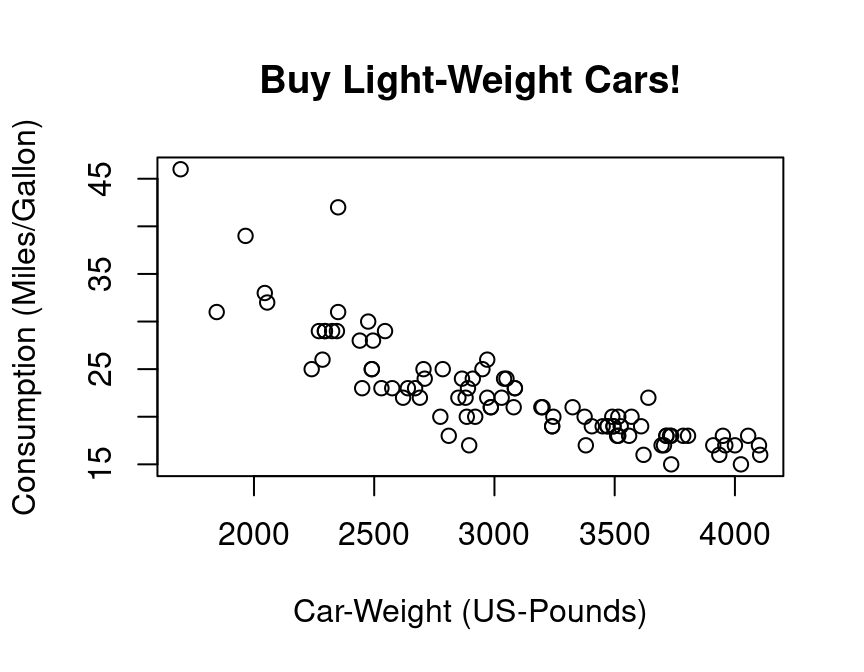
\includegraphics[width=0.8\linewidth]{figure/minimal-fig-margin-1} \end{center}

\hfill\break

As a first step, we might assume a simple kind of linear relationship between the variables \texttt{gasolin.consumption} and \texttt{car.weight}. Let us assume that the data was generated by the following simple regression model:
\[
y_i=\alpha+\beta_1 x_i+\varepsilon_i,\quad i=1,\dots,n
\]
where \(y_i\) denotes the gasoline-consumption, \(x_i\) the weight of car \(i\), and \(\varepsilon_i\) is a mean zero constant variance noise term. (This is clearly a non-sense model!)

The command \texttt{lm()} computes the estimates of this linear regression model. The command (in fact it's a \emph{method}) \texttt{summary()} computes further quantities of general interest from the \emph{object} that was returned from the \texttt{lm()} function.

\begin{Shaded}
\begin{Highlighting}[]
\NormalTok{lm.result   }\OtherTok{\textless{}{-}} \FunctionTok{lm}\NormalTok{(gasolin.consumption}\SpecialCharTok{\textasciitilde{}}\NormalTok{car.weight)}
\NormalTok{lm.summary  }\OtherTok{\textless{}{-}} \FunctionTok{summary}\NormalTok{(lm.result)}
\NormalTok{lm.summary}
\CommentTok{\#\textgreater{} }
\CommentTok{\#\textgreater{} Call:}
\CommentTok{\#\textgreater{} lm(formula = gasolin.consumption \textasciitilde{} car.weight)}
\CommentTok{\#\textgreater{} }
\CommentTok{\#\textgreater{} Residuals:}
\CommentTok{\#\textgreater{}     Min      1Q  Median      3Q     Max }
\CommentTok{\#\textgreater{} {-}6.7946 {-}1.9711  0.0249  1.1855 13.8278 }
\CommentTok{\#\textgreater{} }
\CommentTok{\#\textgreater{} Coefficients:}
\CommentTok{\#\textgreater{}              Estimate Std. Error t value Pr(\textgreater{}|t|)    }
\CommentTok{\#\textgreater{} (Intercept) 47.048353   1.679912   28.01   \textless{}2e{-}16 ***}
\CommentTok{\#\textgreater{} car.weight  {-}0.008032   0.000537  {-}14.96   \textless{}2e{-}16 ***}
\CommentTok{\#\textgreater{} {-}{-}{-}}
\CommentTok{\#\textgreater{} Signif. codes:  0 \textquotesingle{}***\textquotesingle{} 0.001 \textquotesingle{}**\textquotesingle{} 0.01 \textquotesingle{}*\textquotesingle{} 0.05 \textquotesingle{}.\textquotesingle{} 0.1 \textquotesingle{} \textquotesingle{} 1}
\CommentTok{\#\textgreater{} }
\CommentTok{\#\textgreater{} Residual standard error: 3.038 on 91 degrees of freedom}
\CommentTok{\#\textgreater{} Multiple R{-}squared:  0.7109, Adjusted R{-}squared:  0.7077 }
\CommentTok{\#\textgreater{} F{-}statistic: 223.8 on 1 and 91 DF,  p{-}value: \textless{} 2.2e{-}16}
\end{Highlighting}
\end{Shaded}

\hfill\break

Of course, we want to have a possibility to access all the quantities computed so far, e.g., in order to plot the results. This can be done as following:

\begin{Shaded}
\begin{Highlighting}[]
\DocumentationTok{\#\# Accessing the computed quantities}
\FunctionTok{names}\NormalTok{(lm.summary) }\DocumentationTok{\#\# Alternatively: str(lm.summary)}
\CommentTok{\#\textgreater{}  [1] "call"          "terms"         "residuals"     "coefficients"  "aliased"      }
\CommentTok{\#\textgreater{}  [6] "sigma"         "df"            "r.squared"     "adj.r.squared" "fstatistic"   }
\CommentTok{\#\textgreater{} [11] "cov.unscaled"}

\NormalTok{alpha }\OtherTok{\textless{}{-}}\NormalTok{ lm.summary}\SpecialCharTok{$}\NormalTok{coefficients[}\DecValTok{1}\NormalTok{]}
\NormalTok{beta  }\OtherTok{\textless{}{-}}\NormalTok{ lm.summary}\SpecialCharTok{$}\NormalTok{coefficients[}\DecValTok{2}\NormalTok{]}

\DocumentationTok{\#\# Plot all:}
\FunctionTok{plot}\NormalTok{(}\AttributeTok{y=}\NormalTok{gasolin.consumption, }\AttributeTok{x=}\NormalTok{car.weight, }
     \AttributeTok{xlab=}\StringTok{"Car{-}Weight (US{-}Pounds)"}\NormalTok{, }
     \AttributeTok{ylab=}\StringTok{"Consumption (Miles/Gallon)"}\NormalTok{, }
     \AttributeTok{main=}\StringTok{"Buy light{-}weight Cars!"}\NormalTok{)}
\FunctionTok{abline}\NormalTok{(}\AttributeTok{a=}\NormalTok{alpha, }
       \AttributeTok{b=}\NormalTok{beta, }\AttributeTok{col=}\StringTok{"red"}\NormalTok{)}
\end{Highlighting}
\end{Shaded}

\begin{center}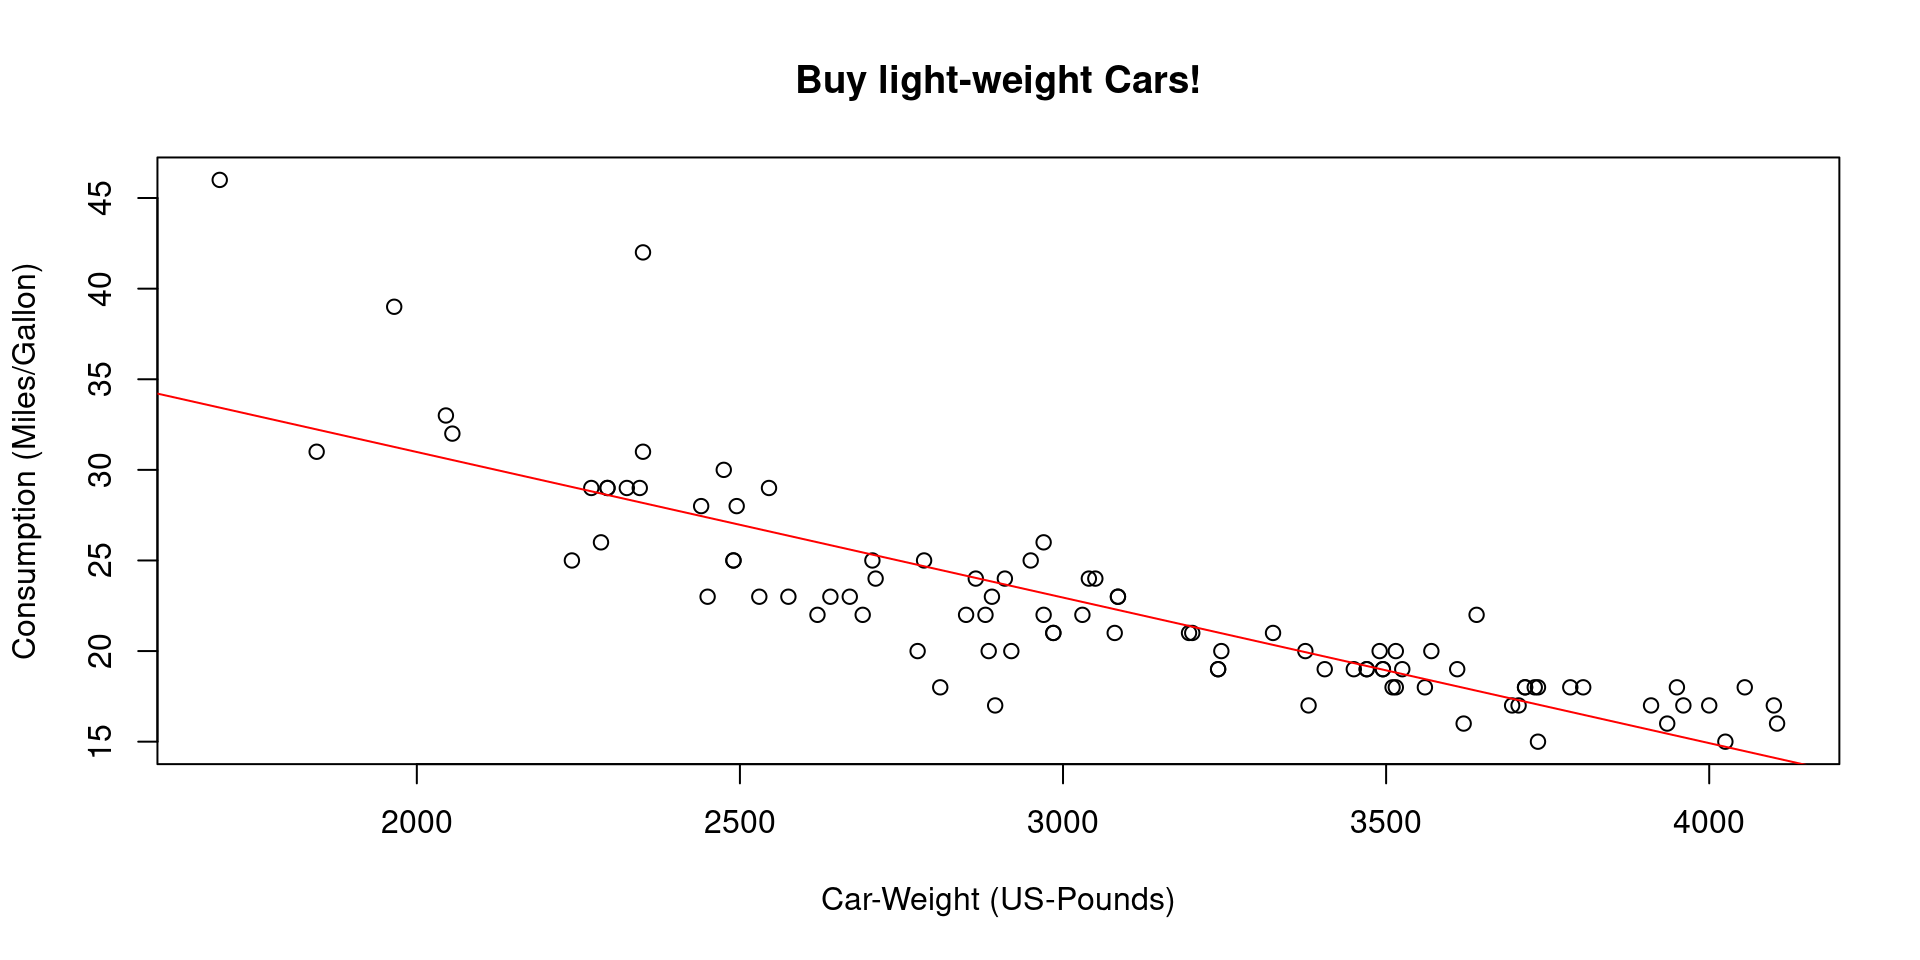
\includegraphics[width=\textwidth]{figure/minimal-unnamed-chunk-25-1} \end{center}

\hfill\break

\hypertarget{programming-in-r}{%
\section{Programming in R}\label{programming-in-r}}

Let's write, i.e., program our own R-function for estimating linear regression models. In order to be able to validate our function, we start with \textbf{simulating data} for which we then \emph{know} all true parameters. Simulating data is like being the ``Data-God'': For instance, we generate realizations of the error term \(\varepsilon_i\), i.e., something which we \emph{never} observe in real data.

\hfill\break

Let us consider the following multiple regression model:

\[y_i=\beta_1 +\beta_2 x_{2i}+\beta_3 x_{3i}+\varepsilon_{i},\quad i=1,\dots,n,\]
where \(\varepsilon_{i}\) is a heteroscedastic error term
\[\varepsilon_{i}\sim N(0,\sigma_i^2),\quad \sigma_i=|x_{3i}|,\]

and where for all \(i=1,\dots,n=50\):

\begin{itemize}
\tightlist
\item
  \(x_{2i}\sim N(10,1.5^2)\)
\item
  \(x_{3i}\) comes from a t-distribution with 5 degrees of freedom and non-centrality parameter 2
\end{itemize}

\begin{Shaded}
\begin{Highlighting}[]
\FunctionTok{set.seed}\NormalTok{(}\DecValTok{109}\NormalTok{) }\CommentTok{\# Sets the "seed" of the random number generators:}
\NormalTok{n   }\OtherTok{\textless{}{-}} \DecValTok{50}     \CommentTok{\# Number of observations}

\DocumentationTok{\#\# Generate two explanatory variables plus an intercept{-}variable:}
\NormalTok{X}\FloatTok{.1} \OtherTok{\textless{}{-}} \FunctionTok{rep}\NormalTok{(}\DecValTok{1}\NormalTok{, n)                 }\CommentTok{\# Intercept}
\NormalTok{X}\FloatTok{.2} \OtherTok{\textless{}{-}} \FunctionTok{rnorm}\NormalTok{(n, }\AttributeTok{mean=}\DecValTok{10}\NormalTok{, }\AttributeTok{sd=}\FloatTok{1.5}\NormalTok{) }\CommentTok{\# Draw realizations form a normal distr.}
\NormalTok{X}\FloatTok{.3} \OtherTok{\textless{}{-}} \FunctionTok{rt}\NormalTok{(n, }\AttributeTok{df=}\DecValTok{5}\NormalTok{, }\AttributeTok{ncp=}\DecValTok{2}\NormalTok{)        }\CommentTok{\# Draw realizations form a t{-}distr.}
\NormalTok{X   }\OtherTok{\textless{}{-}} \FunctionTok{cbind}\NormalTok{(X}\FloatTok{.1}\NormalTok{, X}\FloatTok{.2}\NormalTok{, X}\FloatTok{.3}\NormalTok{)      }\CommentTok{\# Save as a Nx3{-}dimensional data matrix.}
\end{Highlighting}
\end{Shaded}

OK, we have regressors, i.e., data that we also have in real data sets.

Now we define the elements of the \(\beta\)-vector. Be aware of the difference: In real data sets we do not know the true \(\beta\)-vector, but try to estimate it. However, when simulating data, we determine (as ``Data-Gods'') the true \(\beta\)-vector and can compare our estimate \(\hat{\beta}\) with the true \(\beta\):

\begin{Shaded}
\begin{Highlighting}[]
\DocumentationTok{\#\# Define the slope{-}coefficients}
\NormalTok{beta.vec  }\OtherTok{\textless{}{-}} \FunctionTok{c}\NormalTok{(}\DecValTok{1}\NormalTok{,}\SpecialCharTok{{-}}\DecValTok{5}\NormalTok{,}\DecValTok{5}\NormalTok{)}
\end{Highlighting}
\end{Shaded}

\hfill\break
We still need to simulate realizations of the dependent variable \(y_i\). Remember that \(y_i=\beta_1 x_{1i}+\beta_1 x_{2i}+\beta_3 x_{3i}+\varepsilon_{i}\). That is, we only need realizations from the error terms \(\varepsilon_i\) in order to compute the realizations from \(y_i\). This is how you can simulate realizations from the heteroscedastic error terms \(\varepsilon_i\):

\begin{Shaded}
\begin{Highlighting}[]
\DocumentationTok{\#\# Generate realizations from the heteroscadastic error term}
\NormalTok{eps       }\OtherTok{\textless{}{-}} \FunctionTok{abs}\NormalTok{(X}\FloatTok{.3}\NormalTok{) }\SpecialCharTok{*} \FunctionTok{rnorm}\NormalTok{(n, }\AttributeTok{mean=}\DecValTok{0}\NormalTok{, }\AttributeTok{sd=}\DecValTok{1}\NormalTok{)}
\end{Highlighting}
\end{Shaded}

Take a look at the heteroscedasticity in the error term:

\begin{Shaded}
\begin{Highlighting}[]
\FunctionTok{plot}\NormalTok{(}\AttributeTok{y=}\NormalTok{eps, }\AttributeTok{x=}\NormalTok{X}\FloatTok{.3}\NormalTok{, }
     \AttributeTok{main=}\StringTok{"Realizations of the }\SpecialCharTok{\textbackslash{}n}\StringTok{Heteroscedastic Error Term"}\NormalTok{)}
\end{Highlighting}
\end{Shaded}

\begin{center}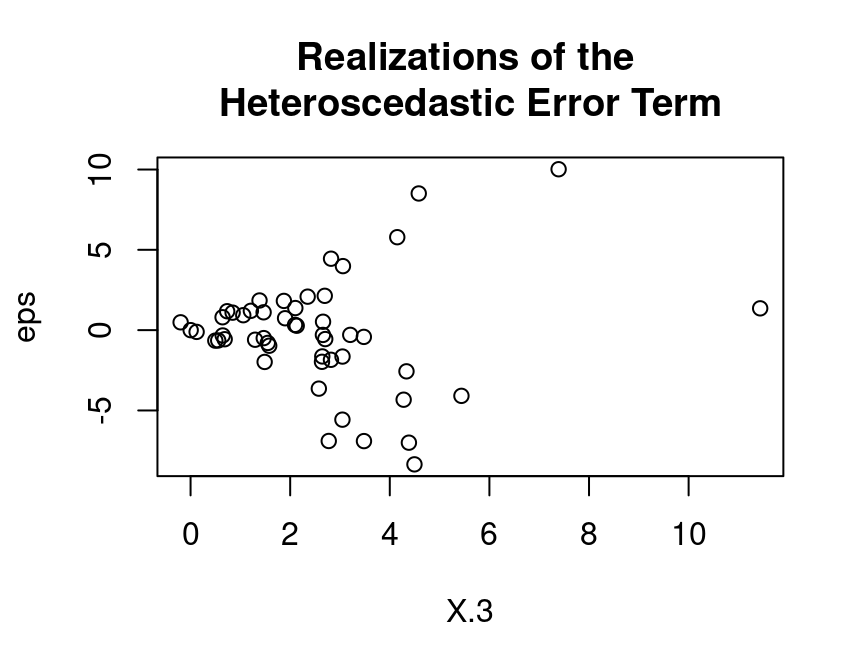
\includegraphics[width=0.8\linewidth]{figure/minimal-unnamed-chunk-29-1} \end{center}

With the (pseudo-random) realizations from \(\varepsilon_i\), we can finally generate realizations from the dependent variable \(y_i\):

\begin{Shaded}
\begin{Highlighting}[]
\DocumentationTok{\#\# Dependent variable:}
\NormalTok{y   }\OtherTok{\textless{}{-}}\NormalTok{ X }\SpecialCharTok{\%*\%}\NormalTok{ beta.vec }\SpecialCharTok{+}\NormalTok{ eps}
\end{Highlighting}
\end{Shaded}

Let's take a look at the data:

\begin{Shaded}
\begin{Highlighting}[]
\NormalTok{mydata    }\OtherTok{\textless{}{-}} \FunctionTok{data.frame}\NormalTok{(}\StringTok{"Y"}\OtherTok{=}\NormalTok{y, }\StringTok{"X.1"}\OtherTok{=}\NormalTok{X}\FloatTok{.1}\NormalTok{, }\StringTok{"X.2"}\OtherTok{=}\NormalTok{X}\FloatTok{.2}\NormalTok{, }\StringTok{"X.3"}\OtherTok{=}\NormalTok{X}\FloatTok{.3}\NormalTok{)}
\FunctionTok{pairs}\NormalTok{(mydata[,}\SpecialCharTok{{-}}\DecValTok{2}\NormalTok{]) }\CommentTok{\# The \textquotesingle{}{-}2\textquotesingle{} removes the intercept variable "X.1"}
\end{Highlighting}
\end{Shaded}

\begin{center}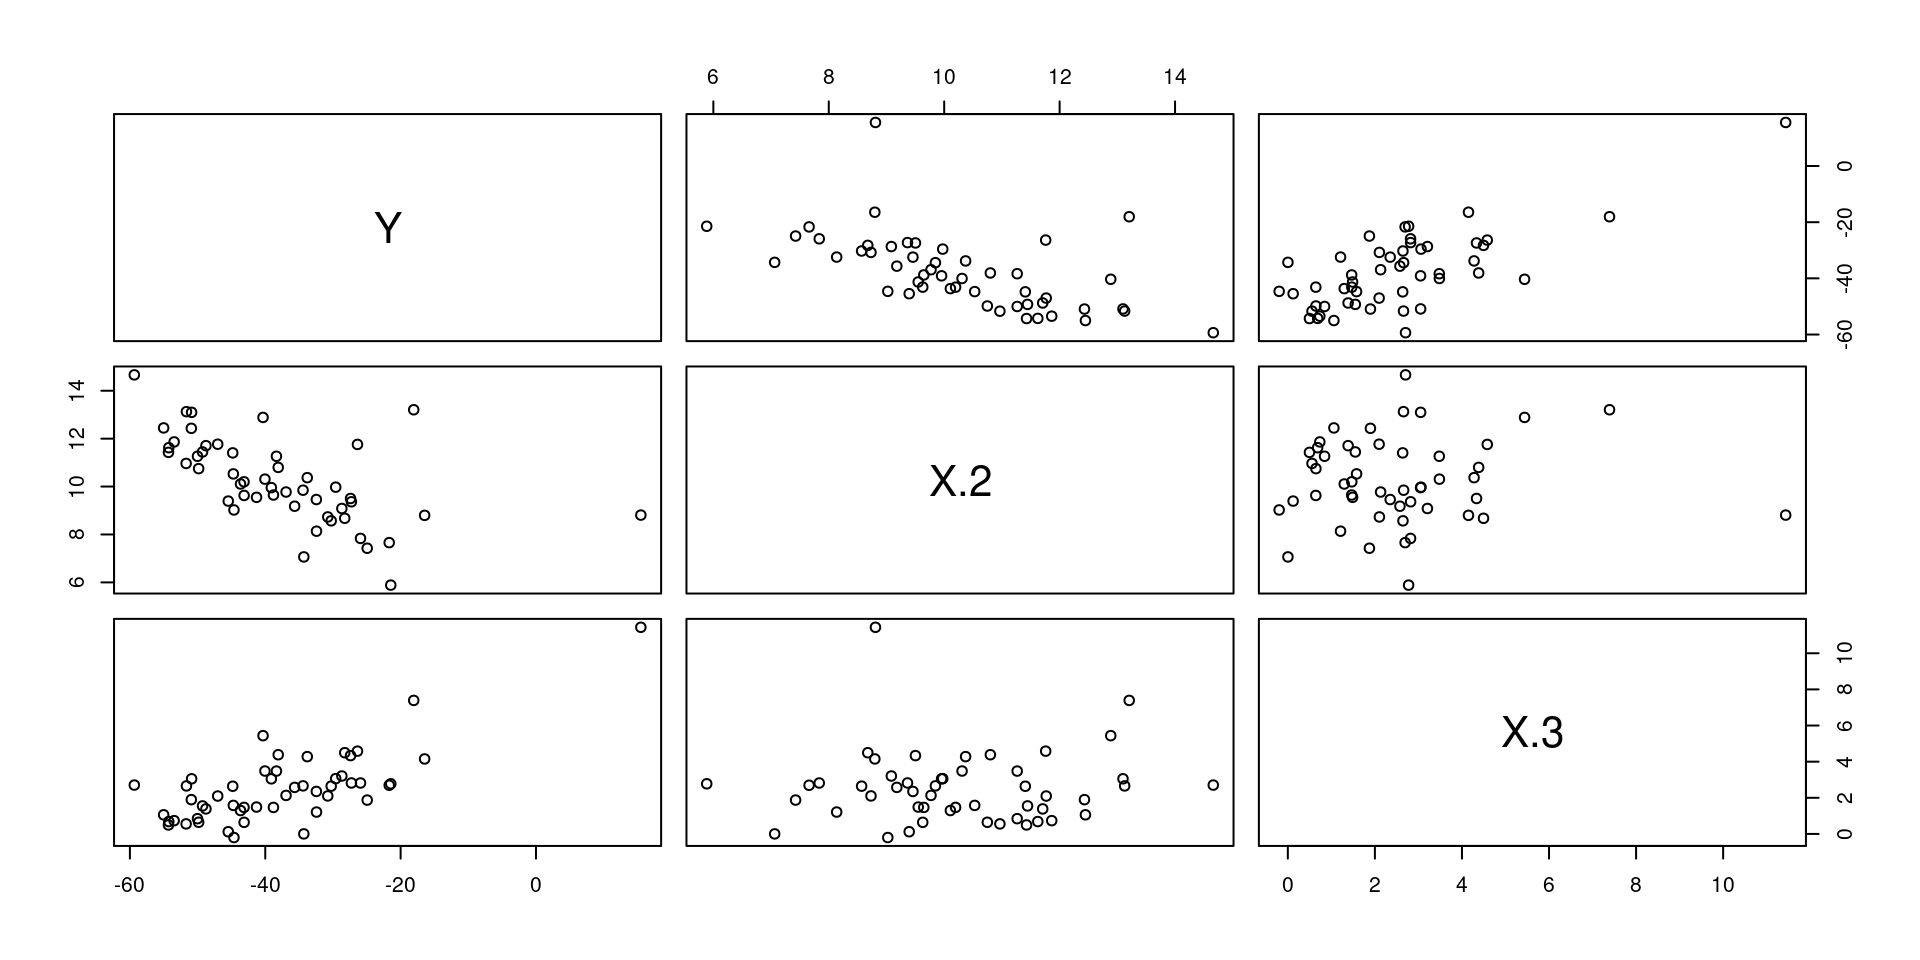
\includegraphics[width=\textwidth]{figure/minimal-unnamed-chunk-31-1} \end{center}

\hfill\break

Once we have data, we can compute the OLS estimate of the true \(\beta\) vector. Remember the formula:
\[\hat{\beta}=(X^\top X)^{-1}X^\top y\]
In R-Code this is: \((X^\top X)^{-1}=\)\texttt{solve(t(X)\ \%*\%\ X)}, i.e.:

\begin{Shaded}
\begin{Highlighting}[]
\DocumentationTok{\#\# Computation of the beta{-}Vector:}
\NormalTok{beta.hat }\OtherTok{\textless{}{-}} \FunctionTok{solve}\NormalTok{(}\FunctionTok{t}\NormalTok{(X) }\SpecialCharTok{\%*\%}\NormalTok{ X) }\SpecialCharTok{\%*\%} \FunctionTok{t}\NormalTok{(X) }\SpecialCharTok{\%*\%}\NormalTok{ y}
\NormalTok{beta.hat}
\CommentTok{\#\textgreater{}          [,1]}
\CommentTok{\#\textgreater{} X.1 {-}2.609634}
\CommentTok{\#\textgreater{} X.2 {-}4.692735}
\CommentTok{\#\textgreater{} X.3  5.078342}
\end{Highlighting}
\end{Shaded}

\hfill\break

Well done. Using the above lines of code we can easily program our own \texttt{myOLSFun()} function!

\begin{Shaded}
\begin{Highlighting}[]
\NormalTok{myOLSFun }\OtherTok{\textless{}{-}} \ControlFlowTok{function}\NormalTok{(y, x, }\AttributeTok{add.intercept=}\ConstantTok{FALSE}\NormalTok{)\{}
  
  \DocumentationTok{\#\# Number of Observations:}
\NormalTok{  n         }\OtherTok{\textless{}{-}} \FunctionTok{length}\NormalTok{(y)}
  
  \DocumentationTok{\#\# Add an intercept to x:}
  \ControlFlowTok{if}\NormalTok{(add.intercept)\{}
\NormalTok{    Intercept }\OtherTok{\textless{}{-}} \FunctionTok{rep}\NormalTok{(}\DecValTok{1}\NormalTok{, n)}
\NormalTok{    x         }\OtherTok{\textless{}{-}} \FunctionTok{cbind}\NormalTok{(Intercept, x)}
\NormalTok{  \}}
  
  \DocumentationTok{\#\# Estimation of the slope{-}parameters:}
\NormalTok{  beta.hat.vec }\OtherTok{\textless{}{-}} \FunctionTok{solve}\NormalTok{(}\FunctionTok{t}\NormalTok{(x) }\SpecialCharTok{\%*\%}\NormalTok{ x) }\SpecialCharTok{\%*\%} \FunctionTok{t}\NormalTok{(x) }\SpecialCharTok{\%*\%}\NormalTok{ y}
  
  \DocumentationTok{\#\# Return the result:}
  \FunctionTok{return}\NormalTok{(beta.hat.vec)}
\NormalTok{\}}

\DocumentationTok{\#\# Run the function:}
\FunctionTok{myOLSFun}\NormalTok{(}\AttributeTok{y=}\NormalTok{y, }\AttributeTok{x=}\NormalTok{X)}
\CommentTok{\#\textgreater{}          [,1]}
\CommentTok{\#\textgreater{} X.1 {-}2.609634}
\CommentTok{\#\textgreater{} X.2 {-}4.692735}
\CommentTok{\#\textgreater{} X.3  5.078342}
\end{Highlighting}
\end{Shaded}

\hfill\break

Can you extend the function for the computation of the covariance matrix of the slope-estimates, several measures of fits (R\(^2\), adj.-R\(^2\), etc.), t-tests, \ldots?

\hypertarget{r-packages}{%
\section{R-packages}\label{r-packages}}

One of the best features in R are its contributed packages. The list of all packages on CRAN is impressive! Take a look at it \href{https://cran.r-project.org/web/packages/available_packages_by_name.html}{HERE}

For instance, nice plots can be produced using the R-package is \texttt{ggplot2}. You can find an intro do this package \href{http://ggplot2.tidyverse.org/}{HERE}.

\begin{Shaded}
\begin{Highlighting}[]
\CommentTok{\# install.packages("ggplot2")}
\FunctionTok{library}\NormalTok{(}\StringTok{"ggplot2"}\NormalTok{)}

\FunctionTok{qplot}\NormalTok{(Sepal.Length, Petal.Length, }\AttributeTok{data =}\NormalTok{ iris, }\AttributeTok{color =}\NormalTok{ Species)}
\end{Highlighting}
\end{Shaded}

\begin{center}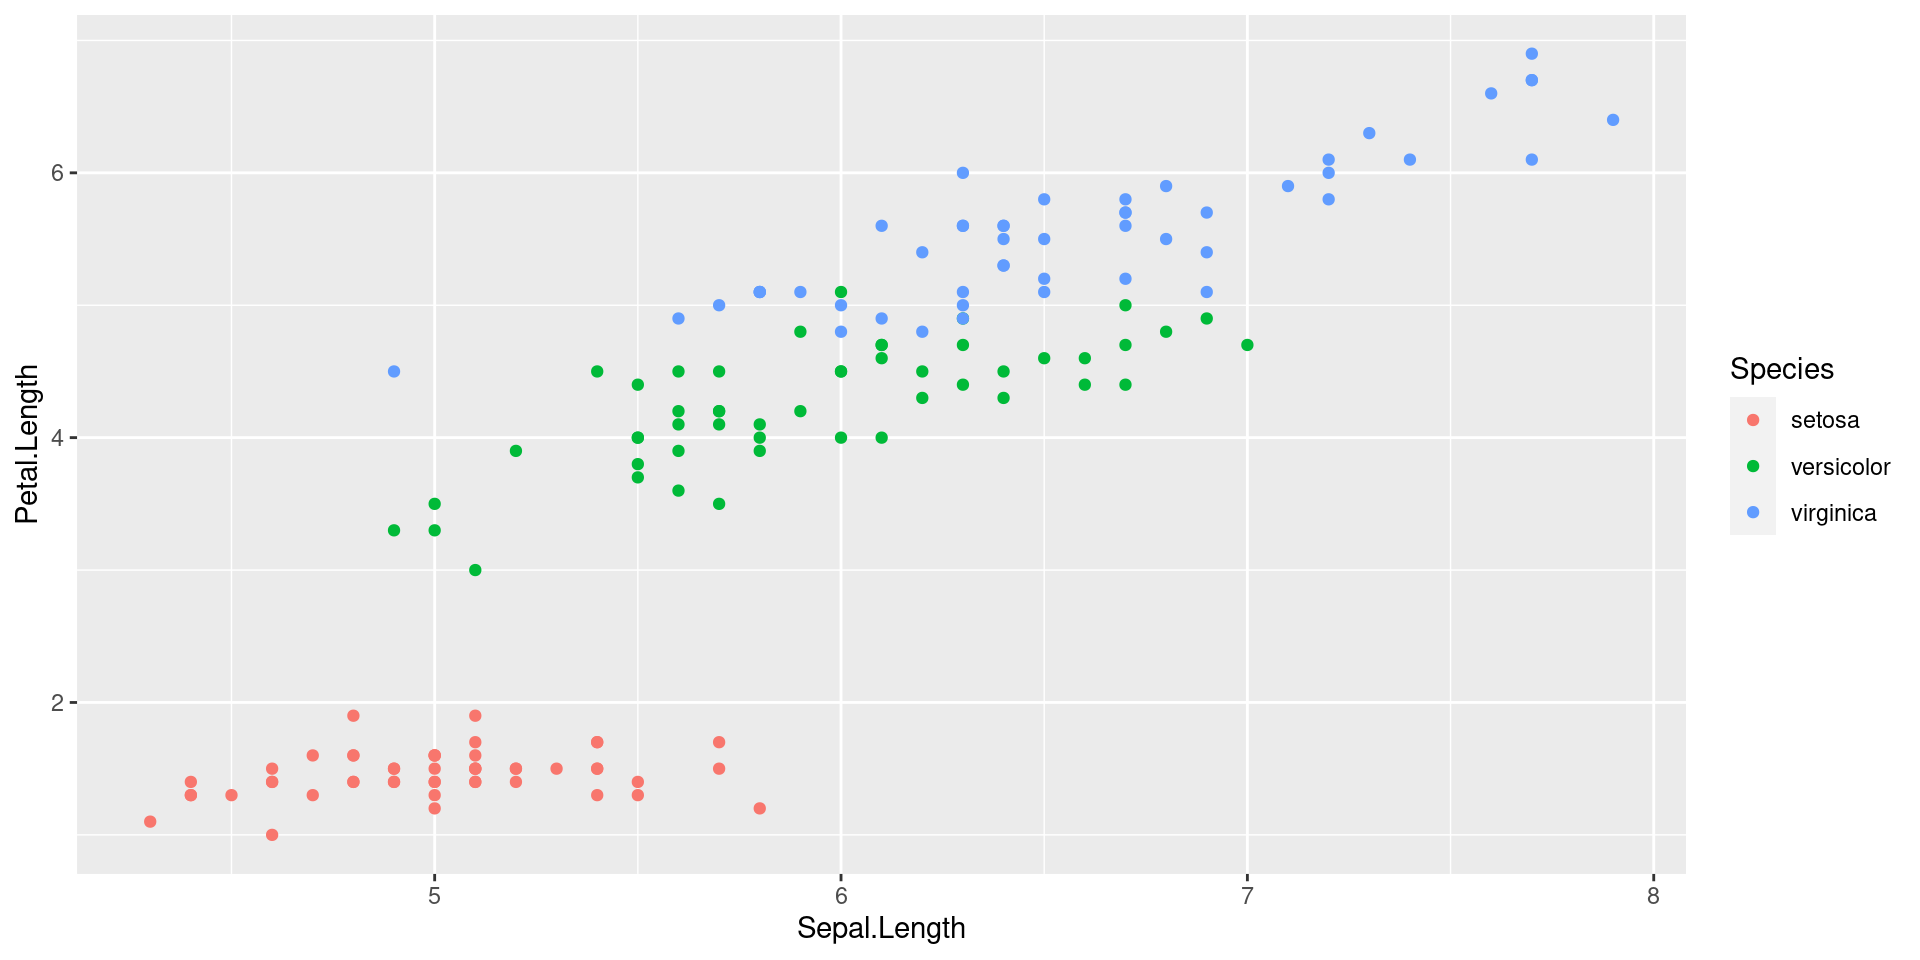
\includegraphics[width=\textwidth]{figure/minimal-unnamed-chunk-34-1} \end{center}

\hfill\break

Of course, \texttt{ggplot2} concerns ``only'' plotting, but you'll find R-packages for almost any statistical method out there.

\hypertarget{tidyverse}{%
\section{Tidyverse}\label{tidyverse}}

The \texttt{tidyverse} package is a collection of packages that lets you import,
manipulate, explore, visualize and model data in a harmonized and consistent way which
helps you to be more productive.

Installing the \texttt{tidyverse} package:

\begin{Shaded}
\begin{Highlighting}[]
\FunctionTok{install.packages}\NormalTok{(}\StringTok{"tidyverse"}\NormalTok{)}
\end{Highlighting}
\end{Shaded}

To use the \texttt{tidyverse} package load it using the \texttt{library()} function:

\begin{Shaded}
\begin{Highlighting}[]
\FunctionTok{library}\NormalTok{(tidyverse)}
\end{Highlighting}
\end{Shaded}

\textbf{Chick Weight Data}

R comes with many datasets installed. We will use the \texttt{ChickWeight} dataset
to learn about the tidyverse. The help system gives a basic summary of the experiment from
which the data was collect:

\begin{quote}
\emph{``The body weights of the chicks were measured at birth and every second day thereafter
until day 20. They were also measured on day 21. There were four groups of chicks on
different protein diets.''}
\end{quote}

You can get more information, including references by typing:

\begin{Shaded}
\begin{Highlighting}[]
\FunctionTok{help}\NormalTok{(}\StringTok{"ChickWeight"}\NormalTok{)}
\end{Highlighting}
\end{Shaded}

\textbf{The Data: }
There are 578 observations (rows) and 4 variables:

\begin{itemize}
\tightlist
\item
  \texttt{Chick} -- unique ID for each chick.
\item
  \texttt{Diet} -- one of four protein diets.
\item
  \texttt{Time} -- number of days since birth.
\item
  \texttt{weight} -- body weight of chick in grams.
\end{itemize}

Note: \texttt{weight} has a lower case \texttt{w} (recall R is case sensitive).

Store the data locally:

\begin{Shaded}
\begin{Highlighting}[]
\NormalTok{ChickWeight }\SpecialCharTok{\%\textgreater{}\%}
  \FunctionTok{select}\NormalTok{(Chick, Diet, Time, weight) }\SpecialCharTok{\%\textgreater{}\%} 
  \FunctionTok{arrange}\NormalTok{(Chick, Diet, Time) }\SpecialCharTok{\%\textgreater{}\%} 
  \FunctionTok{write\_csv}\NormalTok{(}\StringTok{"ChickWeight.csv"}\NormalTok{)}
\end{Highlighting}
\end{Shaded}

First we will import the data from a file called \texttt{ChickWeight.csv} using the \texttt{read\_csv()}
function from the \texttt{readr} package (part of the \texttt{tidyverse}). The first thing to do,
outside of R, is to open the file \texttt{ChickWeight.csv} to check what it contains and that
it makes sense. Now we can import the data as follows:

\begin{Shaded}
\begin{Highlighting}[]
\NormalTok{CW }\OtherTok{\textless{}{-}} \FunctionTok{read\_csv}\NormalTok{(}\StringTok{"ChickWeight.csv"}\NormalTok{)}
\end{Highlighting}
\end{Shaded}

If all goes well then the data is now stored in an R object called \texttt{CW}. If you get the
following error message then you need to change the working directory to where the data is
stored.

\begin{verbatim}
Error: 'ChickWeight.csv' does not exist in current
working directory ...
\end{verbatim}

\textbf{Changing the working directory:}
In RStudio you can use the menu bar (``Session - Set Working Directory - Choose Directory\ldots{}''). Alternatively, you can use the function \texttt{setwd()}.

\hfill\break

\textbf{Looking at the Dataset:}
To look at the data type just type the object (dataset) name:

\begin{Shaded}
\begin{Highlighting}[]
\NormalTok{CW}
\CommentTok{\#\textgreater{} \# A tibble: 578 x 4}
\CommentTok{\#\textgreater{}    Chick  Diet  Time weight}
\CommentTok{\#\textgreater{}    \textless{}dbl\textgreater{} \textless{}dbl\textgreater{} \textless{}dbl\textgreater{}  \textless{}dbl\textgreater{}}
\CommentTok{\#\textgreater{}  1    18     1     0     39}
\CommentTok{\#\textgreater{}  2    18     1     2     35}
\CommentTok{\#\textgreater{}  3    16     1     0     41}
\CommentTok{\#\textgreater{}  4    16     1     2     45}
\CommentTok{\#\textgreater{}  5    16     1     4     49}
\CommentTok{\#\textgreater{}  6    16     1     6     51}
\CommentTok{\#\textgreater{}  7    16     1     8     57}
\CommentTok{\#\textgreater{}  8    16     1    10     51}
\CommentTok{\#\textgreater{}  9    16     1    12     54}
\CommentTok{\#\textgreater{} 10    15     1     0     41}
\CommentTok{\#\textgreater{} \# ... with 568 more rows}
\end{Highlighting}
\end{Shaded}

If there are too many variables then not all them may be printed. To overcome this issue
we can use the \texttt{glimpse()} function which makes it possible to see every column in your
dataset (called a ``data frame'' in R speak).

\begin{Shaded}
\begin{Highlighting}[]
\FunctionTok{glimpse}\NormalTok{(CW)}
\CommentTok{\#\textgreater{} Rows: 578}
\CommentTok{\#\textgreater{} Columns: 4}
\CommentTok{\#\textgreater{} $ Chick  \textless{}dbl\textgreater{} 18, 18, 16, 16, 16, 16, 16, 16, 16, 15, 15, 15, 15, 15, 15, 15, 15, 13, 1\textasciitilde{}}
\CommentTok{\#\textgreater{} $ Diet   \textless{}dbl\textgreater{} 1, 1, 1, 1, 1, 1, 1, 1, 1, 1, 1, 1, 1, 1, 1, 1, 1, 1, 1, 1, 1, 1, 1, 1, 1\textasciitilde{}}
\CommentTok{\#\textgreater{} $ Time   \textless{}dbl\textgreater{} 0, 2, 0, 2, 4, 6, 8, 10, 12, 0, 2, 4, 6, 8, 10, 12, 14, 0, 2, 4, 6, 8, 10\textasciitilde{}}
\CommentTok{\#\textgreater{} $ weight \textless{}dbl\textgreater{} 39, 35, 41, 45, 49, 51, 57, 51, 54, 41, 49, 56, 64, 68, 68, 67, 68, 41, 4\textasciitilde{}}
\end{Highlighting}
\end{Shaded}

The function \texttt{View()} allows for a spread-sheet type of view on the data:

\begin{Shaded}
\begin{Highlighting}[]
\FunctionTok{View}\NormalTok{(CW)}
\end{Highlighting}
\end{Shaded}

\hypertarget{tidyverse-plotting-basics}{%
\subsection{Tidyverse: Plotting Basics}\label{tidyverse-plotting-basics}}

To \textbf{visualise} the chick weight data, we will use the \texttt{ggplot2} package (part of the
\texttt{tidyverse}). Our interest is in seeing how the \emph{weight changes over time for the chicks by
diet}. For the moment don't worry too much about the details just try to build your own
understanding and logic. To learn more try different things even if you get an error
messages.

Let's plot the weight data (vertical axis) over time (horizontal axis).

\begin{Shaded}
\begin{Highlighting}[]
\CommentTok{\# An empty plot (the plot on the left)}
\FunctionTok{ggplot}\NormalTok{(CW, }\FunctionTok{aes}\NormalTok{(Time, weight))  }
\CommentTok{\# With data (the plot on the right)}
\FunctionTok{ggplot}\NormalTok{(CW, }\FunctionTok{aes}\NormalTok{(Time, weight)) }\SpecialCharTok{+} \FunctionTok{geom\_point}\NormalTok{() }
\end{Highlighting}
\end{Shaded}

\begin{center}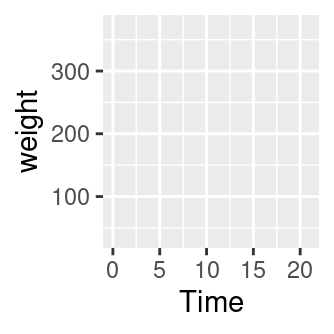
\includegraphics[width=0.8\linewidth]{figure/minimal-emptyPlot-1} 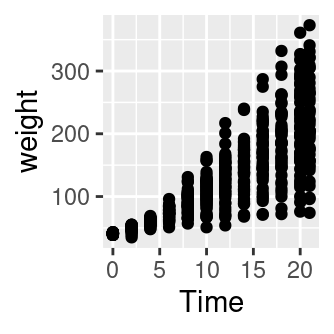
\includegraphics[width=0.8\linewidth]{figure/minimal-emptyPlot-2} \end{center}

Add color for \texttt{Diet}. The graph above does not differentiate between the diets. Let's use a different color for
each diet.

\begin{Shaded}
\begin{Highlighting}[]
\CommentTok{\# Adding colour for diet}
\FunctionTok{ggplot}\NormalTok{(CW,}\FunctionTok{aes}\NormalTok{(Time,weight,}\AttributeTok{colour=}\FunctionTok{factor}\NormalTok{(Diet))) }\SpecialCharTok{+}
  \FunctionTok{geom\_point}\NormalTok{() }
\end{Highlighting}
\end{Shaded}

\begin{center}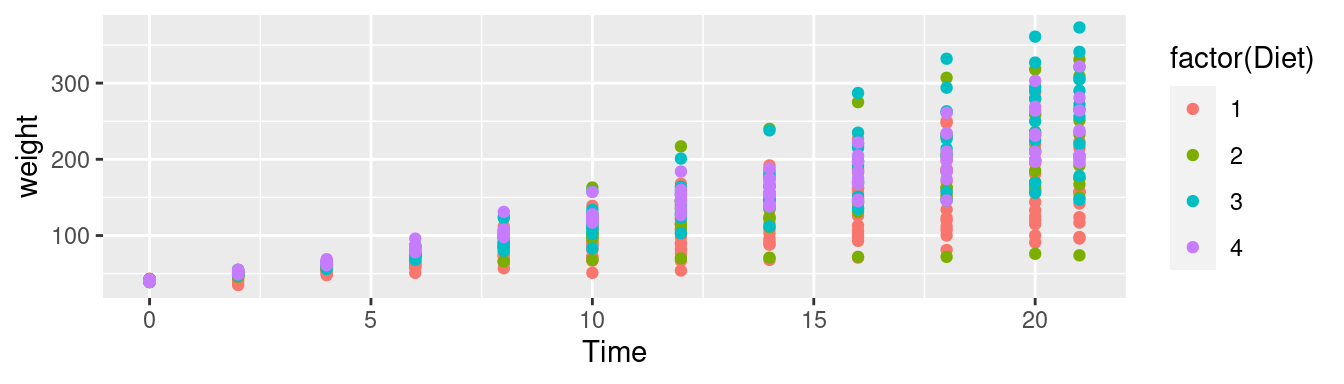
\includegraphics[width=0.8\linewidth]{figure/minimal-addColourPlot-1} \end{center}

It is difficult to conclude anything from this graph as the points are printed on top of
one another (with diet 1 underneath and diet 4 at the top).

\textbf{Factor Variables:}
Before we continue, we have to make an important change to the \texttt{CW} dataset by making
\texttt{Diet} and \texttt{Time} \emph{factor variables}. This means that R will treat them as categorical
variables (see the \texttt{\textless{}fct\textgreater{}} variables below) instead of continuous variables. It will
simplify our coding. The next section will explain the \texttt{mutate()} function.

\begin{Shaded}
\begin{Highlighting}[]
\NormalTok{CW }\OtherTok{\textless{}{-}} \FunctionTok{mutate}\NormalTok{(CW, }\AttributeTok{Diet =} \FunctionTok{factor}\NormalTok{(Diet))}
\NormalTok{CW }\OtherTok{\textless{}{-}} \FunctionTok{mutate}\NormalTok{(CW, }\AttributeTok{Time =} \FunctionTok{factor}\NormalTok{(Time))}
\FunctionTok{glimpse}\NormalTok{(CW)}
\CommentTok{\#\textgreater{} Rows: 578}
\CommentTok{\#\textgreater{} Columns: 4}
\CommentTok{\#\textgreater{} $ Chick  \textless{}dbl\textgreater{} 18, 18, 16, 16, 16, 16, 16, 16, 16, 15, 15, 15, 15, 15, 15, 15, 15, 13, 1\textasciitilde{}}
\CommentTok{\#\textgreater{} $ Diet   \textless{}fct\textgreater{} 1, 1, 1, 1, 1, 1, 1, 1, 1, 1, 1, 1, 1, 1, 1, 1, 1, 1, 1, 1, 1, 1, 1, 1, 1\textasciitilde{}}
\CommentTok{\#\textgreater{} $ Time   \textless{}fct\textgreater{} 0, 2, 0, 2, 4, 6, 8, 10, 12, 0, 2, 4, 6, 8, 10, 12, 14, 0, 2, 4, 6, 8, 10\textasciitilde{}}
\CommentTok{\#\textgreater{} $ weight \textless{}dbl\textgreater{} 39, 35, 41, 45, 49, 51, 57, 51, 54, 41, 49, 56, 64, 68, 68, 67, 68, 41, 4\textasciitilde{}}
\end{Highlighting}
\end{Shaded}

The \texttt{facet\_wrap()} function: To plot each diet separately in a grid using \texttt{facet\_wrap()}:

\begin{Shaded}
\begin{Highlighting}[]
\CommentTok{\# Adding jitter to the points}
\FunctionTok{ggplot}\NormalTok{(CW, }\FunctionTok{aes}\NormalTok{(Time, weight, }\AttributeTok{colour=}\NormalTok{Diet)) }\SpecialCharTok{+}
  \FunctionTok{geom\_point}\NormalTok{() }\SpecialCharTok{+}
  \FunctionTok{facet\_wrap}\NormalTok{(}\SpecialCharTok{\textasciitilde{}}\NormalTok{Diet) }\SpecialCharTok{+}
  \FunctionTok{theme}\NormalTok{(}\AttributeTok{legend.position =} \StringTok{"bottom"}\NormalTok{)}
\end{Highlighting}
\end{Shaded}

\begin{center}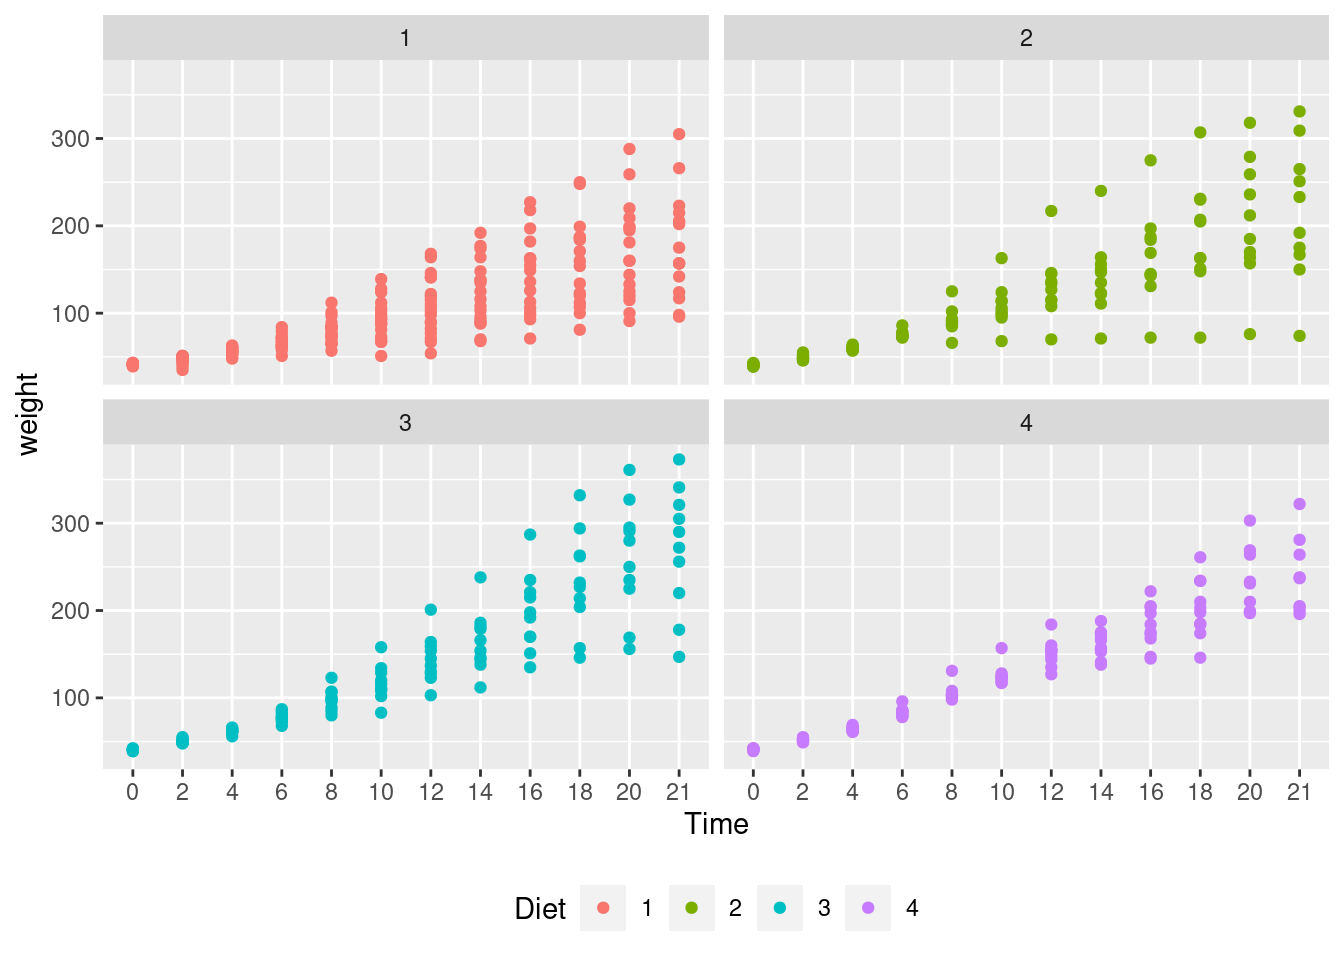
\includegraphics[width=0.8\linewidth]{figure/minimal-ScatterPlot-1} \end{center}

\textbf{Interpretation:} Diet 4 has the least variability but we can't really say anything about the mean effect
of each diet although diet 3 seems to have the highest.

Next we will plot the \textbf{mean changes} over time for each diet using the \texttt{stat\_summary()} function:

\begin{Shaded}
\begin{Highlighting}[]
\FunctionTok{ggplot}\NormalTok{(CW, }\FunctionTok{aes}\NormalTok{(Time, weight, }
               \AttributeTok{group=}\NormalTok{Diet, }\AttributeTok{colour=}\NormalTok{Diet)) }\SpecialCharTok{+}
  \FunctionTok{stat\_summary}\NormalTok{(}\AttributeTok{fun=}\StringTok{"mean"}\NormalTok{, }\AttributeTok{geom=}\StringTok{"line"}\NormalTok{) }
\end{Highlighting}
\end{Shaded}

\begin{center}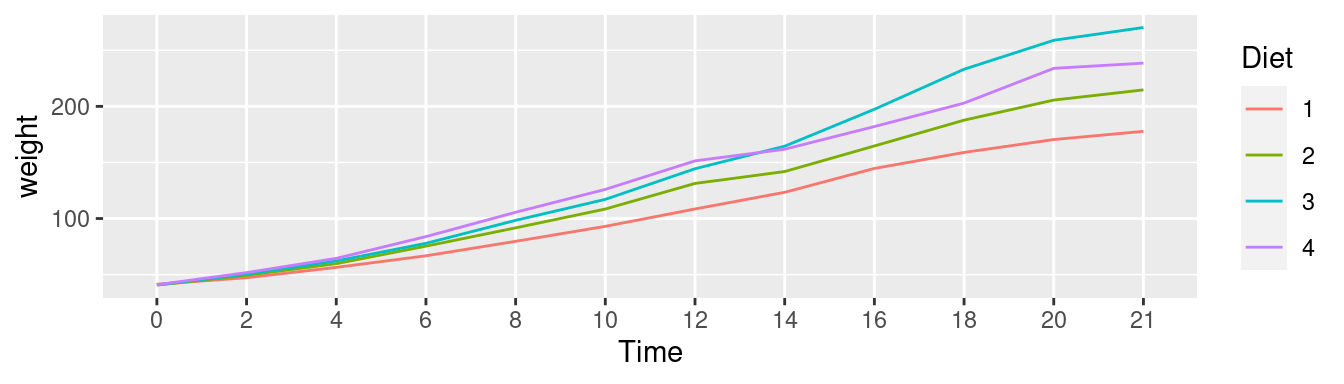
\includegraphics[width=0.8\linewidth]{figure/minimal-meanlinesPlot-1} \end{center}

\textbf{Interpretation:}
We can see that diet 3 has the highest mean weight gains by the end of the experiment. However,
we don't have any information about the variation (uncertainty) in the data.

To see variation between the different diets we use \texttt{geom\_boxplot} to plot a box-whisker plot.
A note of caution is that the number of chicks per diet is relatively low to produce this plot.

\begin{Shaded}
\begin{Highlighting}[]
\FunctionTok{ggplot}\NormalTok{(CW, }\FunctionTok{aes}\NormalTok{(Time, weight, }\AttributeTok{colour=}\NormalTok{Diet)) }\SpecialCharTok{+}
  \FunctionTok{facet\_wrap}\NormalTok{(}\SpecialCharTok{\textasciitilde{}}\NormalTok{Diet) }\SpecialCharTok{+}
  \FunctionTok{geom\_boxplot}\NormalTok{() }\SpecialCharTok{+}
  \FunctionTok{theme}\NormalTok{(}\AttributeTok{legend.position =} \StringTok{"none"}\NormalTok{) }\SpecialCharTok{+}
  \FunctionTok{ggtitle}\NormalTok{(}\StringTok{"Chick Weight over Time by Diet"}\NormalTok{)}
\end{Highlighting}
\end{Shaded}

\begin{center}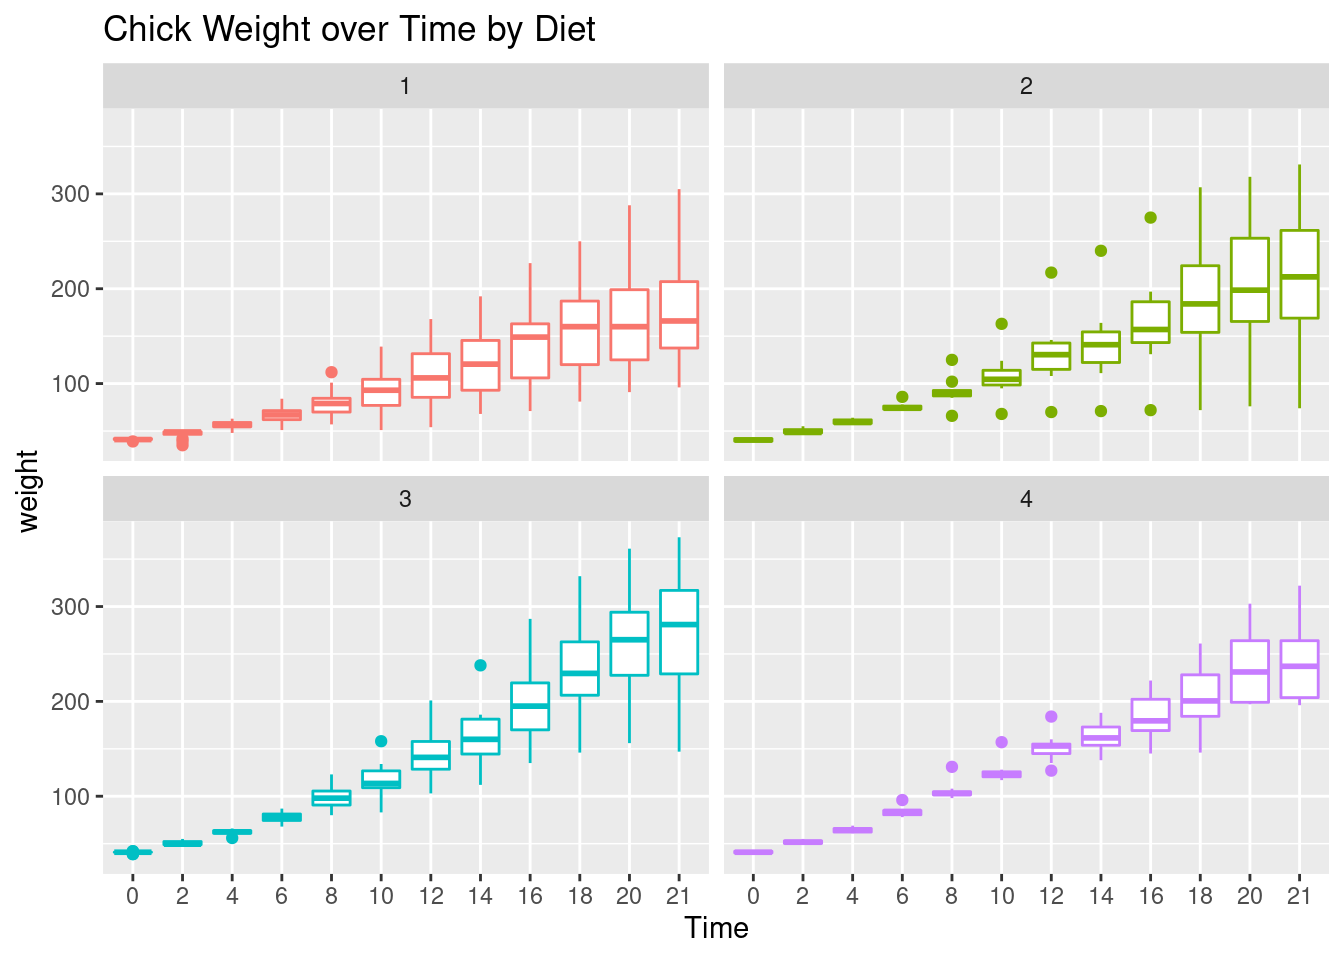
\includegraphics[width=0.8\linewidth]{figure/minimal-boxPlot-1} \end{center}

\textbf{Interpretation:}
Diet 3 seems to have the highest ``average'' weight gain but it has more variation
than diet 4 which is consistent with our findings so far.

Let's finish with a plot that you might include in a publication.

\begin{Shaded}
\begin{Highlighting}[]
\FunctionTok{ggplot}\NormalTok{(CW, }\FunctionTok{aes}\NormalTok{(Time, weight, }\AttributeTok{group=}\NormalTok{Diet, }
                             \AttributeTok{colour=}\NormalTok{Diet)) }\SpecialCharTok{+}
  \FunctionTok{facet\_wrap}\NormalTok{(}\SpecialCharTok{\textasciitilde{}}\NormalTok{Diet) }\SpecialCharTok{+}
  \FunctionTok{geom\_point}\NormalTok{() }\SpecialCharTok{+}
  \CommentTok{\# geom\_jitter() +}
  \FunctionTok{stat\_summary}\NormalTok{(}\AttributeTok{fun=}\StringTok{"mean"}\NormalTok{, }\AttributeTok{geom=}\StringTok{"line"}\NormalTok{,}
               \AttributeTok{colour=}\StringTok{"black"}\NormalTok{) }\SpecialCharTok{+}
  \FunctionTok{theme}\NormalTok{(}\AttributeTok{legend.position =} \StringTok{"none"}\NormalTok{) }\SpecialCharTok{+}
  \FunctionTok{ggtitle}\NormalTok{(}\StringTok{"Chick Weight over Time by Diet"}\NormalTok{) }\SpecialCharTok{+} 
  \FunctionTok{xlab}\NormalTok{(}\StringTok{"Time (days)"}\NormalTok{) }\SpecialCharTok{+}
  \FunctionTok{ylab}\NormalTok{(}\StringTok{"Weight (grams)"}\NormalTok{)}
\end{Highlighting}
\end{Shaded}

\begin{center}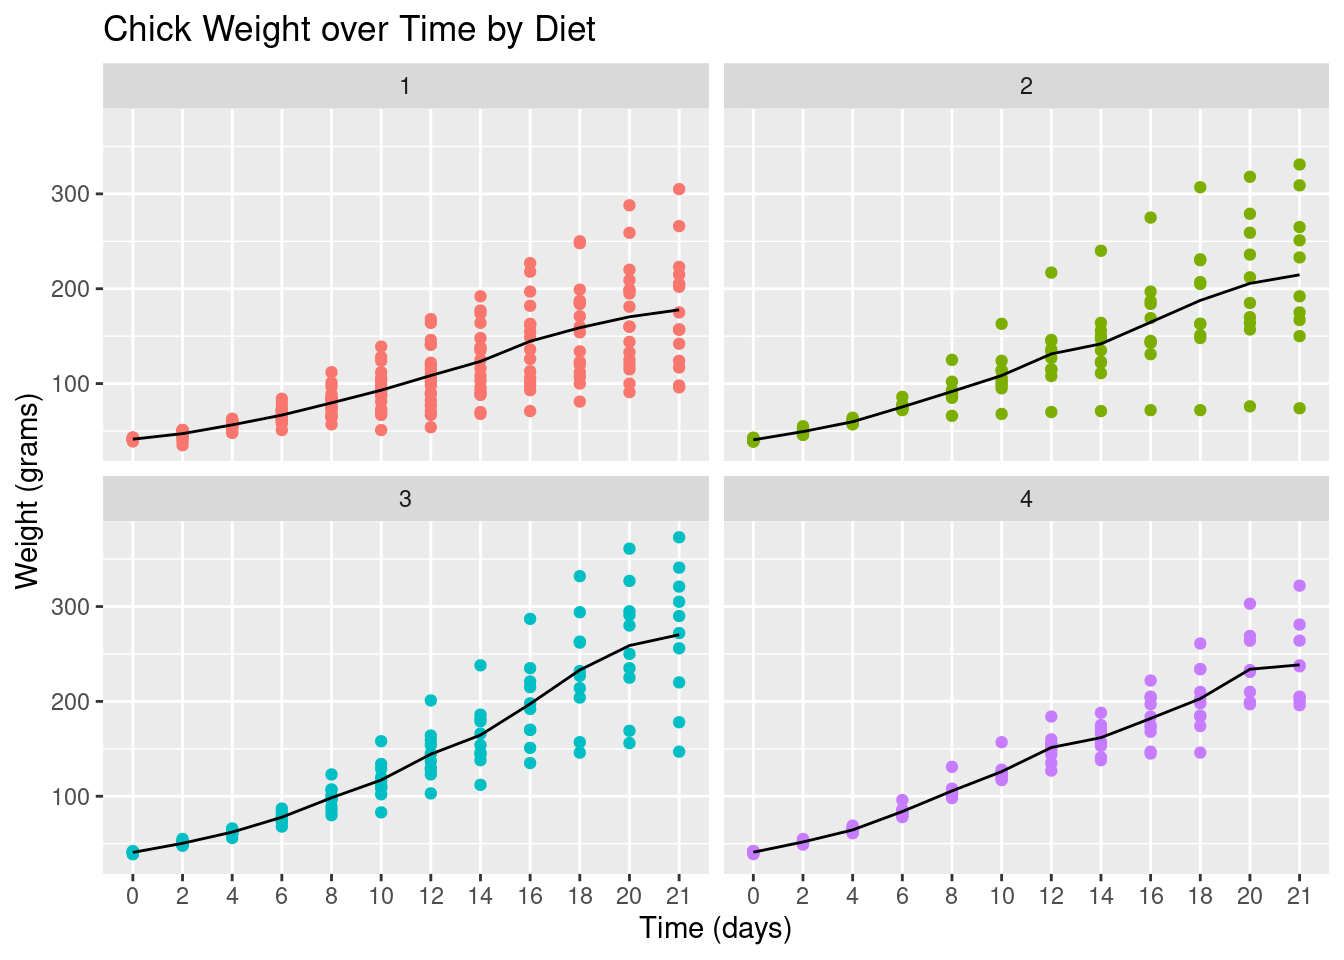
\includegraphics[width=0.8\linewidth]{figure/minimal-finalPlot-1} \end{center}

\hypertarget{tidyverse-data-wrangling-basics}{%
\subsection{Tidyverse: Data Wrangling Basics}\label{tidyverse-data-wrangling-basics}}

In this section we will learn how to wrangle (manipulate) datasets using the \texttt{tidyverse}
package. Let's start with the \texttt{mutate()}, \texttt{select()}, \texttt{rename()}, \texttt{filter()} and \texttt{arrange()}
functions.

\hfill\break

\texttt{mutate()}: Adds a new variable (column) or modifies an existing one. We already used this above to create
factor variables.

\begin{Shaded}
\begin{Highlighting}[]
\CommentTok{\# Added a column}
\NormalTok{CWm1 }\OtherTok{\textless{}{-}} \FunctionTok{mutate}\NormalTok{(CW, }\AttributeTok{weightKg =}\NormalTok{ weight}\SpecialCharTok{/}\DecValTok{1000}\NormalTok{)}
\NormalTok{CWm1}
\CommentTok{\#\textgreater{} \# A tibble: 578 x 5}
\CommentTok{\#\textgreater{}   Chick Diet  Time  weight weightKg}
\CommentTok{\#\textgreater{}   \textless{}dbl\textgreater{} \textless{}fct\textgreater{} \textless{}fct\textgreater{}  \textless{}dbl\textgreater{}    \textless{}dbl\textgreater{}}
\CommentTok{\#\textgreater{} 1    18 1     0         39    0.039}
\CommentTok{\#\textgreater{} 2    18 1     2         35    0.035}
\CommentTok{\#\textgreater{} 3    16 1     0         41    0.041}
\CommentTok{\#\textgreater{} \# ... with 575 more rows}
\CommentTok{\# Modify an existing column}
\NormalTok{CWm2 }\OtherTok{\textless{}{-}} \FunctionTok{mutate}\NormalTok{(CW, }\AttributeTok{Diet =} \FunctionTok{str\_c}\NormalTok{(}\StringTok{"Diet "}\NormalTok{, Diet))}
\NormalTok{CWm2}
\CommentTok{\#\textgreater{} \# A tibble: 578 x 4}
\CommentTok{\#\textgreater{}   Chick Diet   Time  weight}
\CommentTok{\#\textgreater{}   \textless{}dbl\textgreater{} \textless{}chr\textgreater{}  \textless{}fct\textgreater{}  \textless{}dbl\textgreater{}}
\CommentTok{\#\textgreater{} 1    18 Diet 1 0         39}
\CommentTok{\#\textgreater{} 2    18 Diet 1 2         35}
\CommentTok{\#\textgreater{} 3    16 Diet 1 0         41}
\CommentTok{\#\textgreater{} \# ... with 575 more rows}
\end{Highlighting}
\end{Shaded}

\hfill\break

\texttt{select()}: Keeps, drops or reorders variables.

\begin{Shaded}
\begin{Highlighting}[]
\CommentTok{\# Drop the weight variable from CWm1 using minus}
\FunctionTok{select}\NormalTok{(CWm1, }\SpecialCharTok{{-}}\NormalTok{weight)}
\CommentTok{\#\textgreater{} \# A tibble: 578 x 4}
\CommentTok{\#\textgreater{}   Chick Diet  Time  weightKg}
\CommentTok{\#\textgreater{}   \textless{}dbl\textgreater{} \textless{}fct\textgreater{} \textless{}fct\textgreater{}    \textless{}dbl\textgreater{}}
\CommentTok{\#\textgreater{} 1    18 1     0        0.039}
\CommentTok{\#\textgreater{} 2    18 1     2        0.035}
\CommentTok{\#\textgreater{} 3    16 1     0        0.041}
\CommentTok{\#\textgreater{} \# ... with 575 more rows}
\CommentTok{\# Keep variables Time, Diet and weightKg}
\FunctionTok{select}\NormalTok{(CWm1, Chick, Time, Diet, weightKg)}
\CommentTok{\#\textgreater{} \# A tibble: 578 x 4}
\CommentTok{\#\textgreater{}   Chick Time  Diet  weightKg}
\CommentTok{\#\textgreater{}   \textless{}dbl\textgreater{} \textless{}fct\textgreater{} \textless{}fct\textgreater{}    \textless{}dbl\textgreater{}}
\CommentTok{\#\textgreater{} 1    18 0     1        0.039}
\CommentTok{\#\textgreater{} 2    18 2     1        0.035}
\CommentTok{\#\textgreater{} 3    16 0     1        0.041}
\CommentTok{\#\textgreater{} \# ... with 575 more rows}
\end{Highlighting}
\end{Shaded}

\hfill\break

\texttt{rename()}: Renames variables whilst keeping all variables.

\begin{Shaded}
\begin{Highlighting}[]
\FunctionTok{rename}\NormalTok{(CW, }\AttributeTok{Group =}\NormalTok{ Diet, }\AttributeTok{Weight =}\NormalTok{ weight)}
\CommentTok{\#\textgreater{} \# A tibble: 578 x 4}
\CommentTok{\#\textgreater{}   Chick Group Time  Weight}
\CommentTok{\#\textgreater{}   \textless{}dbl\textgreater{} \textless{}fct\textgreater{} \textless{}fct\textgreater{}  \textless{}dbl\textgreater{}}
\CommentTok{\#\textgreater{} 1    18 1     0         39}
\CommentTok{\#\textgreater{} 2    18 1     2         35}
\CommentTok{\#\textgreater{} 3    16 1     0         41}
\CommentTok{\#\textgreater{} \# ... with 575 more rows}
\end{Highlighting}
\end{Shaded}

\hfill\break

\texttt{filter()}: Keeps or drops observations (rows).

\begin{Shaded}
\begin{Highlighting}[]
\FunctionTok{filter}\NormalTok{(CW, Time}\SpecialCharTok{==}\DecValTok{21} \SpecialCharTok{\&}\NormalTok{ weight}\SpecialCharTok{\textgreater{}}\DecValTok{300}\NormalTok{)}
\CommentTok{\#\textgreater{} \# A tibble: 8 x 4}
\CommentTok{\#\textgreater{}   Chick Diet  Time  weight}
\CommentTok{\#\textgreater{}   \textless{}dbl\textgreater{} \textless{}fct\textgreater{} \textless{}fct\textgreater{}  \textless{}dbl\textgreater{}}
\CommentTok{\#\textgreater{} 1     7 1     21       305}
\CommentTok{\#\textgreater{} 2    29 2     21       309}
\CommentTok{\#\textgreater{} 3    21 2     21       331}
\CommentTok{\#\textgreater{} \# ... with 5 more rows}
\end{Highlighting}
\end{Shaded}

For comparing values in vectors use: \texttt{\textless{}} (less than), \texttt{\textgreater{}} (greater than), \texttt{\textless{}=}
(less than and equal to), \texttt{\textgreater{}=} (greater than and equal to), \texttt{==} (equal to) and \texttt{!=}
(not equal to). These can be combined logically using \texttt{\&} (and) and \texttt{\textbar{}} (or).

\hfill\break

\texttt{arrange()}: Changes the order of the observations.

\begin{Shaded}
\begin{Highlighting}[]
\FunctionTok{arrange}\NormalTok{(CW, Chick, Time)}
\CommentTok{\#\textgreater{} \# A tibble: 578 x 4}
\CommentTok{\#\textgreater{}   Chick Diet  Time  weight}
\CommentTok{\#\textgreater{}   \textless{}dbl\textgreater{} \textless{}fct\textgreater{} \textless{}fct\textgreater{}  \textless{}dbl\textgreater{}}
\CommentTok{\#\textgreater{} 1     1 1     0         42}
\CommentTok{\#\textgreater{} 2     1 1     2         51}
\CommentTok{\#\textgreater{} 3     1 1     4         59}
\CommentTok{\#\textgreater{} \# ... with 575 more rows}
\FunctionTok{arrange}\NormalTok{(CW, }\FunctionTok{desc}\NormalTok{(weight))}
\CommentTok{\#\textgreater{} \# A tibble: 578 x 4}
\CommentTok{\#\textgreater{}   Chick Diet  Time  weight}
\CommentTok{\#\textgreater{}   \textless{}dbl\textgreater{} \textless{}fct\textgreater{} \textless{}fct\textgreater{}  \textless{}dbl\textgreater{}}
\CommentTok{\#\textgreater{} 1    35 3     21       373}
\CommentTok{\#\textgreater{} 2    35 3     20       361}
\CommentTok{\#\textgreater{} 3    34 3     21       341}
\CommentTok{\#\textgreater{} \# ... with 575 more rows}
\end{Highlighting}
\end{Shaded}

What does the \texttt{desc()} do? Try using \texttt{desc(Time)}.

\hypertarget{the-pipe-operator}{%
\subsection{\texorpdfstring{The pipe operator \texttt{\%\textgreater{}\%}}{The pipe operator \%\textgreater\%}}\label{the-pipe-operator}}

In reality you will end up doing multiple data wrangling steps that you want to save.
The pipe operator \texttt{\%\textgreater{}\%} makes your code nice and readable:

\begin{Shaded}
\begin{Highlighting}[]
\NormalTok{CW21 }\OtherTok{\textless{}{-}}\NormalTok{ CW }\SpecialCharTok{\%\textgreater{}\%} 
  \FunctionTok{filter}\NormalTok{(Time }\SpecialCharTok{\%in\%} \FunctionTok{c}\NormalTok{(}\DecValTok{0}\NormalTok{, }\DecValTok{21}\NormalTok{)) }\SpecialCharTok{\%\textgreater{}\%} 
  \FunctionTok{rename}\NormalTok{(}\AttributeTok{Weight =}\NormalTok{ weight) }\SpecialCharTok{\%\textgreater{}\%} 
  \FunctionTok{mutate}\NormalTok{(}\AttributeTok{Group =} \FunctionTok{factor}\NormalTok{(}\FunctionTok{str\_c}\NormalTok{(}\StringTok{"Diet "}\NormalTok{, Diet))) }\SpecialCharTok{\%\textgreater{}\%} 
  \FunctionTok{select}\NormalTok{(Chick, Group, Time, Weight) }\SpecialCharTok{\%\textgreater{}\%} 
  \FunctionTok{arrange}\NormalTok{(Chick, Time) }
\NormalTok{CW21}
\CommentTok{\#\textgreater{} \# A tibble: 95 x 4}
\CommentTok{\#\textgreater{}   Chick Group  Time  Weight}
\CommentTok{\#\textgreater{}   \textless{}dbl\textgreater{} \textless{}fct\textgreater{}  \textless{}fct\textgreater{}  \textless{}dbl\textgreater{}}
\CommentTok{\#\textgreater{} 1     1 Diet 1 0         42}
\CommentTok{\#\textgreater{} 2     1 Diet 1 21       205}
\CommentTok{\#\textgreater{} 3     2 Diet 1 0         40}
\CommentTok{\#\textgreater{} \# ... with 92 more rows}
\end{Highlighting}
\end{Shaded}

Hint: To understand the code above we should read the pipe operator \texttt{\%\textgreater{}\%} as ``then''.

\begin{quote}
Create a new dataset (object) called \texttt{CW21} using dataset \texttt{CW} \textbf{\emph{then}}
keep the data for days 0 and 21 \textbf{\emph{then}} rename variable \texttt{weight} to \texttt{Weight}
\textbf{\emph{then}} create a variable called \texttt{Group} \textbf{\emph{then}} keep variables \texttt{Chick},
\texttt{Group}, \texttt{Time} and \texttt{Weight} and \textbf{\emph{then}} finally arrange the data by
variables \texttt{Chick} and \texttt{Time}.
\end{quote}

This is the same code:

\begin{Shaded}
\begin{Highlighting}[]
\NormalTok{CW21 }\OtherTok{\textless{}{-}}\NormalTok{ CW }\SpecialCharTok{\%\textgreater{}\%} 
  \FunctionTok{filter}\NormalTok{(., Time }\SpecialCharTok{\%in\%} \FunctionTok{c}\NormalTok{(}\DecValTok{0}\NormalTok{, }\DecValTok{21}\NormalTok{)) }\SpecialCharTok{\%\textgreater{}\%} 
  \FunctionTok{rename}\NormalTok{(., }\AttributeTok{Weight =}\NormalTok{ weight) }\SpecialCharTok{\%\textgreater{}\%} 
  \FunctionTok{mutate}\NormalTok{(., }\AttributeTok{Group=}\FunctionTok{factor}\NormalTok{(}\FunctionTok{str\_c}\NormalTok{(}\StringTok{"Diet "}\NormalTok{,Diet))) }\SpecialCharTok{\%\textgreater{}\%} 
  \FunctionTok{select}\NormalTok{(., Chick, Group, Time, Weight) }\SpecialCharTok{\%\textgreater{}\%} 
  \FunctionTok{arrange}\NormalTok{(., Chick, Time) }
\end{Highlighting}
\end{Shaded}

The pipe operator, \texttt{\%\textgreater{}\%}, replaces the dots (\texttt{.}) with whatever is returned from code
preceding it. For example, the dot in \texttt{filter(.,\ Time\ \%in\%\ c(0,\ 21))} is replaced by
\texttt{CW}. The output of the \texttt{filter(...)} then replaces the dot in
\texttt{rename(.,\ Weight\ =\ weight)} and so on. Think of it as a data assembly line with
each function doing its thing and passing it to the next.

\hypertarget{the-group_by-function}{%
\subsection{\texorpdfstring{The \texttt{group\_by()} function}{The group\_by() function}}\label{the-group_by-function}}

From the data visualizations above we concluded that the diet 3 has the highest mean
and diet 4 the least variation. In this section, we will quantify the effects of the
diets using \textbf{summmary statistics}. We start by looking at the number of observations
and the mean by \textbf{diet} and \textbf{time}.

\begin{Shaded}
\begin{Highlighting}[]
\NormalTok{mnsdCW }\OtherTok{\textless{}{-}}\NormalTok{ CW }\SpecialCharTok{\%\textgreater{}\%} 
  \FunctionTok{group\_by}\NormalTok{(Diet, Time) }\SpecialCharTok{\%\textgreater{}\%} 
  \FunctionTok{summarise}\NormalTok{(}\AttributeTok{N =} \FunctionTok{n}\NormalTok{(), }\AttributeTok{Mean =} \FunctionTok{mean}\NormalTok{(weight)) }\SpecialCharTok{\%\textgreater{}\%} 
  \FunctionTok{arrange}\NormalTok{(Diet, Time)}
\NormalTok{mnsdCW}
\CommentTok{\#\textgreater{} \# A tibble: 48 x 4}
\CommentTok{\#\textgreater{} \# Groups:   Diet [4]}
\CommentTok{\#\textgreater{}   Diet  Time      N  Mean}
\CommentTok{\#\textgreater{}   \textless{}fct\textgreater{} \textless{}fct\textgreater{} \textless{}int\textgreater{} \textless{}dbl\textgreater{}}
\CommentTok{\#\textgreater{} 1 1     0        20  41.4}
\CommentTok{\#\textgreater{} 2 1     2        20  47.2}
\CommentTok{\#\textgreater{} 3 1     4        19  56.5}
\CommentTok{\#\textgreater{} \# ... with 45 more rows}
\end{Highlighting}
\end{Shaded}

For each distinct combination of \texttt{Diet} and \texttt{Time}, the chick weight data is summarized
into the number of observations (\texttt{N}) and the mean (\texttt{Mean}) of \texttt{weight}.

\textbf{Further summaries:} Let's also calculate the standard deviation, median, minimum and maximum values but only
at days 0 and 21.

\begin{Shaded}
\begin{Highlighting}[]
\NormalTok{sumCW }\OtherTok{\textless{}{-}}\NormalTok{  CW }\SpecialCharTok{\%\textgreater{}\%} 
  \FunctionTok{filter}\NormalTok{(Time }\SpecialCharTok{\%in\%} \FunctionTok{c}\NormalTok{(}\DecValTok{0}\NormalTok{, }\DecValTok{21}\NormalTok{)) }\SpecialCharTok{\%\textgreater{}\%} 
  \FunctionTok{group\_by}\NormalTok{(Diet, Time) }\SpecialCharTok{\%\textgreater{}\%} 
  \FunctionTok{summarise}\NormalTok{(}\AttributeTok{N =} \FunctionTok{n}\NormalTok{(),}
            \AttributeTok{Mean =} \FunctionTok{mean}\NormalTok{(weight),}
            \AttributeTok{SD =} \FunctionTok{sd}\NormalTok{(weight),}
            \AttributeTok{Median =} \FunctionTok{median}\NormalTok{(weight),}
            \AttributeTok{Min =} \FunctionTok{min}\NormalTok{(weight),}
            \AttributeTok{Max =} \FunctionTok{max}\NormalTok{(weight)) }\SpecialCharTok{\%\textgreater{}\%} 
  \FunctionTok{arrange}\NormalTok{(Diet, Time)}
\NormalTok{sumCW}
\CommentTok{\#\textgreater{} \# A tibble: 8 x 8}
\CommentTok{\#\textgreater{} \# Groups:   Diet [4]}
\CommentTok{\#\textgreater{}   Diet  Time      N  Mean     SD Median   Min   Max}
\CommentTok{\#\textgreater{}   \textless{}fct\textgreater{} \textless{}fct\textgreater{} \textless{}int\textgreater{} \textless{}dbl\textgreater{}  \textless{}dbl\textgreater{}  \textless{}dbl\textgreater{} \textless{}dbl\textgreater{} \textless{}dbl\textgreater{}}
\CommentTok{\#\textgreater{} 1 1     0        20  41.4  0.995   41      39    43}
\CommentTok{\#\textgreater{} 2 1     21       16 178.  58.7    166      96   305}
\CommentTok{\#\textgreater{} 3 2     0        10  40.7  1.49    40.5    39    43}
\CommentTok{\#\textgreater{} \# ... with 5 more rows}
\end{Highlighting}
\end{Shaded}

Let's make the summaries ``prettier'', say, for a report or publication.

\begin{Shaded}
\begin{Highlighting}[]
\FunctionTok{library}\NormalTok{(}\StringTok{"knitr"}\NormalTok{) }\CommentTok{\# to use the kable() function}
\NormalTok{prettySumCW }\OtherTok{\textless{}{-}}\NormalTok{ sumCW }\SpecialCharTok{\%\textgreater{}\%} 
 \FunctionTok{mutate}\NormalTok{(}\StringTok{\textasciigrave{}}\AttributeTok{Mean (SD)}\StringTok{\textasciigrave{}} \OtherTok{=} \FunctionTok{str\_c}\NormalTok{(}\FunctionTok{format}\NormalTok{(Mean, }\AttributeTok{digits=}\DecValTok{1}\NormalTok{),}
           \StringTok{" ("}\NormalTok{, }\FunctionTok{format}\NormalTok{(SD, }\AttributeTok{digits=}\DecValTok{2}\NormalTok{), }\StringTok{")"}\NormalTok{)) }\SpecialCharTok{\%\textgreater{}\%} 
 \FunctionTok{mutate}\NormalTok{(}\AttributeTok{Range =} \FunctionTok{str\_c}\NormalTok{(Min, }\StringTok{" {-} "}\NormalTok{, Max)) }\SpecialCharTok{\%\textgreater{}\%} 
 \FunctionTok{select}\NormalTok{(Diet, Time, N, }\StringTok{\textasciigrave{}}\AttributeTok{Mean (SD)}\StringTok{\textasciigrave{}}\NormalTok{, Median, Range) }\SpecialCharTok{\%\textgreater{}\%}
 \FunctionTok{arrange}\NormalTok{(Diet, Time) }\SpecialCharTok{\%\textgreater{}\%} 
 \FunctionTok{kable}\NormalTok{(}\AttributeTok{format =} \StringTok{"latex"}\NormalTok{)}
\NormalTok{prettySumCW}
\end{Highlighting}
\end{Shaded}

\begin{tabular}{l|l|r|l|r|l}
\hline
Diet & Time & N & Mean (SD) & Median & Range\\
\hline
1 & 0 & 20 & 41 ( 0.99) & 41.0 & 39 - 43\\
\hline
1 & 21 & 16 & 178 (58.70) & 166.0 & 96 - 305\\
\hline
2 & 0 & 10 & 41 ( 1.5) & 40.5 & 39 - 43\\
\hline
2 & 21 & 10 & 215 (78.1) & 212.5 & 74 - 331\\
\hline
3 & 0 & 10 & 41 ( 1) & 41.0 & 39 - 42\\
\hline
3 & 21 & 10 & 270 (72) & 281.0 & 147 - 373\\
\hline
4 & 0 & 10 & 41 ( 1.1) & 41.0 & 39 - 42\\
\hline
4 & 21 & 9 & 239 (43.3) & 237.0 & 196 - 322\\
\hline
\end{tabular}

\textbf{Interpretation:}
This summary table offers the same interpretation as before, namely that diet 3 has the
highest mean and median weights at day 21 but a higher variation than group 4.
However it should be noted that at day 21, diet 1 lost 4 chicks from 20 that started
and diet 4 lost 1 from 10. This could be a sign of some health related issues.

\hypertarget{further-links}{%
\section{Further Links}\label{further-links}}

\hypertarget{further-r-intros}{%
\subsection{Further R-Intros}\label{further-r-intros}}

\begin{itemize}
\item
  \url{https://eddelbuettel.github.io/gsir-te/Getting-Started-in-R.pdf}
\item
  \url{https://www.datacamp.com/courses/free-introduction-to-r}
\item
  \url{https://swcarpentry.github.io/r-novice-gapminder/}
\item
  \url{https://support.rstudio.com/hc/en-us/articles/200526207-Using-Projects}
\end{itemize}

\hypertarget{version-control-gitgithub}{%
\subsection{Version Control (Git/GitHub)}\label{version-control-gitgithub}}

\begin{itemize}
\item
  \url{https://support.rstudio.com/hc/en-us/articles/200532077-Version-Control-with-Git-and-SVN}
\item
  \url{http://happygitwithr.com/}
\item
  \url{https://www.gitkraken.com/}
\end{itemize}

\hypertarget{r-ladies}{%
\subsection{R-Ladies}\label{r-ladies}}

\begin{itemize}
\tightlist
\item
  \url{https://rladies.org/}
\end{itemize}

\hypertarget{ReviewStats}{%
\chapter{Review: Probability and Statistics}\label{ReviewStats}}

\hypertarget{probability-theory}{%
\section{Probability Theory}\label{probability-theory}}

Probability is the mathematical language for quantifying uncertainty. We can apply probability theory to a diverse set of problems, from coin flipping to the analysis of econometric problems. The starting point is to specify the \textbf{sample space}, that is, the set of possible outcomes.

\hypertarget{sample-spaces-and-elementary-events}{%
\subsection{Sample Spaces and (Elementary) Events}\label{sample-spaces-and-elementary-events}}

The \textbf{sample space} \(\Omega,\) is the set of possible outcomes of an experiment. Points \(\omega\) in \(\Omega\) are called \textbf{sample outcomes} or \textbf{realizations} or \textbf{elementary events}. \textbf{Events} are subsets of \(\Omega\).

\bigskip

\noindent\textbf{Example:} If we toss a coin twice then \(\Omega=\{H H, H T, T H, T T\} .\) The event that the first toss is heads is \(A=\{H H, H T\}\).

\bigskip

\noindent\textbf{Example:} Let \(\omega\) be the outcome of a measurement of some physical quantity, for example, temperature. Then \(\Omega=\mathbb{R}=(-\infty, \infty).\) The event that the measurement is larger than 10 but less than or equal to 23 is \(A=(10,23]\).

\bigskip

\noindent\textbf{Example:} If we toss a coin forever then the sample space is the infinite set \(\Omega=\left\{\omega=\left(\omega_{1}, \omega_{2}, \omega_{3}, \ldots,\right)|\omega_{i} \in\{H, T\}\right\}\) Let \(A\) be the event that the first head appears on the third toss. Then
\(A=\left\{\left(\omega_{1}, \omega_{2}, \omega_{3}, \ldots,\right)| \omega_{1}=T, \omega_{2}=T, \omega_{3}=H, \omega_{i} \in\{H, T\} \text { for } i>3\right\}\).

\bigskip

Given an event \(A,\) let \(A^{c}=\{\omega \in \Omega ; \omega \notin A\}\) denote the \textbf{complement} of \(A\). Informally, \(A^{c}\) can be read as \say{not $A$.} The complement of \(\Omega\) is the empty set \(\emptyset\). The \textbf{union} of events \(A\) and \(B\) is defined as
\[
A\cup B=\{\omega \in \Omega|\omega\in A\text{ or }\omega \in B\text{ or }\omega\in\text{ both}\}
\]
which can be thought of as \say{$A$ or $B$.} If \(A_{1}, A_{2}, \ldots\) is a sequence of sets then
\[
\bigcup_{i=1}^{\infty} A_{i}=\left\{\omega \in \Omega: \omega \in A_{i} \text { for at least one i }\right\}.
\]
The \textbf{intersection} of \(A\) and \(B\) is defined as
\[
A \cap B=\{\omega \in \Omega ; \omega \in A\text{ and }\omega \in B\}\]
which reads as \say{$A$ and $B$.} Sometimes \(A \cap B\) is also written shortly as \(AB\). If \(A_{1}, A_{2}, \ldots\) is a sequence of sets then
\[
\bigcap_{i=1}^{\infty} A_{i}=\left\{\omega \in \Omega: \omega \in A_{i} \text { for all i }\right\}.
\]
If every element of \(A\) is also contained in \(B\) we write \(A \subset B\) or, equivalently, \(B \supset A\). If \(A\) is a finite set, let \(|A|\) denote the number of elements in \(A .\) We say that \(A_{1}, A_{2}, \ldots\) are \textbf{disjoint} or \textbf{mutually exclusive} if \(A_{i} \cap A_{j}=\emptyset\) whenever \(i \neq j\). For example, \(A_{1}=[0,1), A_{2}=[1,2), A_{3}=[2,3), \ldots\) are disjoint. A \textbf{partition} of \(\Omega\) is a sequence of disjoint sets \(A_{1}, A_{2}, \ldots\) such that \(\bigcup_{i=1}^{\infty} A_{i}=\Omega\).

\noindent\textbf{Summary: Sample space and events}
\vspace*{-1cm}

\begin{center}
$$
\begin{array}{ll}
%\multicolumn{2}{l}{\noindent\textbf{Summary: Sample space and events}}\\
\Omega & \text { sample space } \\
\omega & \text { outcome }\\
A      & \text { event (subset of } \Omega) \\
|A|    & \text { number of points in } A \text { (if } A \text { is finite) }\\
A^{c}  & \text { complement of } A (\operatorname{not} A)\\
A \cup B &\text{ union }(A\text{ or }B)\\
A \cap B &\text{ intersection }(A \text { and } B);\text{ short notation: }AB\\
A \subset B &\text{ set inclusion }(A \text{ is a subset of or equal to }B)\\
\emptyset   &\text{ null event (always false)}\\
\Omega      &\text{ true event (always true)}
\end{array}
$$
\end{center}

\hypertarget{probability}{%
\subsection{Probability}\label{probability}}

We want to assign a real number \(P(A)\) to every event \(A,\) called the \textbf{probability} of \(A .\) We also call \(P\) a \textbf{probability distribution} or a \textbf{probability measure}. To qualify as a probability, \(P\) has to satisfy three axioms. That is, a function \(P\) that assigns a real number \(P(A)\in[0,1]\) to each event \(A\) is a \textbf{probability distribution} or a \textbf{probability measure} if it satisfies the following three axioms:
\vspace*{-.25cm}

\begin{description}
\item[Axiom 1:] $P(A) \geq 0$ for every $A$ 
\item[Axiom 2:] $P(\Omega)=1$
\item[Axiom 3:] If $A_{1}, A_{2}, \ldots$ are disjoint then
$$
P\left(\bigcup_{i=1}^{\infty} A_{i}\right)=\sum_{i=1}^{\infty} P\left(A_{i}\right).
$$
\end{description}

\bigskip

\noindent\textbf{Note:} It is not always possible to assign a probability to every event \(A\) if the sample space is large, such as, for instance, the whole real line, \(\Omega=\mathbb{R}\). In case of \(\Omega=\mathbb{R}\) strange things can happen. There are pathological sets that simply break down the mathematics. An example of one of these pathological sets, also known as non-measurable sets because they literally can't be measured (i.e.~we cannot assign probabilities to them), are the Vitali sets. Therefore, in such cases like \(\Omega=\mathbb{R}\), we assign probabilities to a \emph{limited} class of sets called a \textbf{\(\sigma\)-field} or \textbf{\(\sigma\)-algebra}. For \(\Omega=\mathbb{R}\), the canonical \textbf{\(\sigma\)-algebra} is the \textbf{Borel \(\sigma\)-algebra}. The Borel \(\sigma\)-algebra on \(\mathbb{R}\) is generated by the collection of all open subsets of \(R\).

\bigskip

One can derive many properties of \(P\) from the axioms. Here are a few:

\begin{itemize}
\item $P(\emptyset)=0$
\item $A \subset B\Rightarrow P(A) \leq P(B)$
\item $0 \leq P(A) \leq 1$
\item $P\left(A^{c}\right)=1-P(A)$
\item $A \cap B=\emptyset \Rightarrow P(A \cup B)=P(A)+P(B)$
\end{itemize}

A less obvious property is given in the following: For any events \(A\) and \(B\) we have that,
\[P(A \cup B)=P(A)+P(B)-P(A B).\]

\paragraph*{Example.}

Two consecutive coin tosses. Let \(H_{1}\) be the event that heads occurs on toss 1 and let \(H_{2}\) be the event that heads occurs on toss 2. If all outcomes are equally likely, that is, \(\mathrm{P}\left(\left\{H_{1}, H_{2}\right\}\right)=\mathrm{P}\left(\left\{H_{1}, T_{2}\right\}\right)=\mathrm{P}\left(\left\{T_{1}, H_{2}\right\}\right)=\mathrm{P}\left(\left\{T_{1}, T_{2}\right\}\right)=1 / 4\), then
\[
\mathrm{P}\left(H_{1} \cup H_{2}\right)=\mathrm{P}\left(H_{1}\right)+\mathrm{P}\left(H_{2}\right)-\mathrm{P}\left(H_{1} H_{2}\right)=\frac{1}{2}+\frac{1}{2}-\frac{1}{4}=\frac{3}{4}.
\]

\bigskip

\paragraph*{Probailities as frequencies.}

One can interpret \(P(A)\) in terms of \textbf{frequencies}. That is, \(P(A)\) is the (infinitely) long run proportion of times that \(A\) is true in repetitions. For example, if we say that the probability of heads is \(1 / 2\), i.e \(P(H)=1/2\) we mean that if we flip the coin many times then the proportion of times we get heads tends to \(1 / 2\) as the number of tosses increases. An infinitely long, unpredictable sequence of tosses whose limiting proportion tends to a constant is an idealization, much like the idea of a straight line in geometry. \newline
The following \textsf{R} codes approximates the probability \(P(H)=1/2\) using 5, 50 and 5,000 many (pseudo) random coin flips:

\begin{Shaded}
\begin{Highlighting}[]
\FunctionTok{set.seed}\NormalTok{(}\DecValTok{869}\NormalTok{)}
\DocumentationTok{\#\# 1 (fair) coin{-}flip:}
\NormalTok{results }\OtherTok{\textless{}{-}} \FunctionTok{sample}\NormalTok{(}\AttributeTok{x =} \FunctionTok{c}\NormalTok{(}\StringTok{"H"}\NormalTok{, }\StringTok{"T"}\NormalTok{), }\AttributeTok{size =} \DecValTok{5}\NormalTok{, }\AttributeTok{replace =} \ConstantTok{TRUE}\NormalTok{)}
\DocumentationTok{\#\# Relative frequency of "H" in 5 coin{-}flips}
\FunctionTok{length}\NormalTok{(results[results}\SpecialCharTok{==}\StringTok{"H"}\NormalTok{])}\SpecialCharTok{/}\DecValTok{5}
\CommentTok{\#\textgreater{} [1] 0.2}

\DocumentationTok{\#\# 10 (fair) coin{-}flips:}
\NormalTok{results }\OtherTok{\textless{}{-}} \FunctionTok{sample}\NormalTok{(}\AttributeTok{x =} \FunctionTok{c}\NormalTok{(}\StringTok{"H"}\NormalTok{, }\StringTok{"T"}\NormalTok{), }\AttributeTok{size =} \DecValTok{50}\NormalTok{, }\AttributeTok{replace =} \ConstantTok{TRUE}\NormalTok{)}
\DocumentationTok{\#\# Relative frequency of "H" in 50 coin{-}flips}
\FunctionTok{length}\NormalTok{(results[results}\SpecialCharTok{==}\StringTok{"H"}\NormalTok{])}\SpecialCharTok{/}\DecValTok{50}
\CommentTok{\#\textgreater{} [1] 0.52}

\DocumentationTok{\#\# 100000 (fair) coin{-}flips:}
\NormalTok{results }\OtherTok{\textless{}{-}} \FunctionTok{sample}\NormalTok{(}\AttributeTok{x =} \FunctionTok{c}\NormalTok{(}\StringTok{"H"}\NormalTok{, }\StringTok{"T"}\NormalTok{), }\AttributeTok{size =} \DecValTok{5000}\NormalTok{, }\AttributeTok{replace =} \ConstantTok{TRUE}\NormalTok{)}
\DocumentationTok{\#\# Relative frequency of "H" in 5000 coin{-}flips}
\FunctionTok{length}\NormalTok{(results[results}\SpecialCharTok{==}\StringTok{"H"}\NormalTok{])}\SpecialCharTok{/}\DecValTok{5000}
\CommentTok{\#\textgreater{} [1] 0.5024}
\end{Highlighting}
\end{Shaded}

\hypertarget{independent-events}{%
\subsection{Independent Events}\label{independent-events}}

If we flip a fair coin twice, then the probability of two heads is \(\frac{1}{2} \times \frac{1}{2}\). We multiply the probabilities because we regard the two tosses as independent. Two events \(A\) and \(B\) are called \textbf{independent} if
\[P(A B)=P(A) P(B).\]
Or more generally, a whole set of events \(\{A_i|i\in I\}\) is independent if
\[
P\left(\bigcap_{i \in J} A_{i}\right)=\prod_{i \in J}P\left(A_{i}\right)
\]
for every finite subset \(J\) of \(I\), where \(I\) denotes the not necessarily finite index set (e.g.~\(I=\{1,2,\dots\}\)).

\bigskip

Independence can arise in two distinct ways. Sometimes, we \textbf{explicitly assume} that two events are independent. For example, in tossing a coin twice, we usually assume the tosses are independent which reflects the fact that the coin has no memory of the first toss. \newline 
In other instances, we \textbf{derive} independence by verifying that the definition of independence \(P(A B)=P(A)P(B)\) holds. For example, in tossing a fair die \textit{once}, let \(A=\{2,4,6\}\) be the event of observing an even number and let \(B=\{1,2,3,4\}\) be the event of observing no \(5\) and no \(6\). Then,
\(A \cap B=\{2,4\}\) is the event of observing either a \(2\) or a \(4\). Are the events \(A\) and \(B\) independent?\\
\[
P(A B)=\frac{2}{6}=P(A)P(B)=\frac{1}{2}\cdot \frac{2}{3}
\]
and so \(A\) and \(B\) are independent. In this case, we didn't assume that \(A\) and \(B\) are independent it just turned out that they were.

\bigskip

\paragraph*{Cautionary Notes.}

Suppose that \(A\) and \(B\) are \textbf{disjoint events} (i.e.~\(AB=\emptyset\)), each with positive probability (i.e.~\(P(A)>0\) and \(P(B)>0\)). Can they be independent? No! This follows since
\[
P(A B)=P(\emptyset)=0\neq P(A)P(B)>0.
\]
Except in this special case, there is no way to judge (in-)dependence by looking at the sets in a Venn diagram.

\bigskip

\paragraph*{Summary: Independence}
\vspace{-.3cm}

\begin{enumerate}
\def\labelenumi{\arabic{enumi}.}
\tightlist
\item
  \(A\) and \(B\) are independent if \(P(A B)=P(A) P(B)\).
\item
  Independence is sometimes assumed and sometimes derived.
\item
  Disjoint events with strictly positive probabilities are not independent.
\end{enumerate}

\hypertarget{conditional-probability}{%
\subsection{Conditional Probability}\label{conditional-probability}}

If \(P(B)>0\) then the \textbf{conditional probability} of \(A\) given \(B\) is
\[
P(A \mid B)=\frac{P(A B)}{P(B)}.
\]
Think of \(P(A \mid B)\) as the fraction of times \(A\) occurs among those in which \(B\) occurs. Here are some facts about conditional probabilities:

\begin{itemize}
\item The rules of probability apply to events on the left of the bar \say{$\mid$}. That is, for any fixed $B$ such that $P(B)>0, P(\cdot \mid B)$ is a probability i.e. it satisfies the three axioms of probability: $P(A \mid B) \geq 0, P(\Omega \mid B)=1$ and if $A_{1}, A_{2}, \ldots$ are disjoint then $P\left(\bigcup_{i=1}^{\infty} A_{i} \mid B\right)=\sum_{i=1}^{\infty} P\left(A_{i} \mid B\right)$.
\item But it's generally not true that $P(A \mid B \cup C)=P(A \mid B)+P(A \mid C)$. 
\end{itemize}

In general it is also \textbf{not} the case that \(P(A \mid B)=P(B \mid A)\). People get this confused all the time. For example, the probability of spots given you have measles is 1 but the probability that you have measles given that you have spots is not \(1 .\) In this case, the difference between \(P(A \mid B)\) and \(P(B \mid A)\) is obvious but there are cases where it is less obvious. This mistake is made often enough in legal cases that it is sometimes called the \say{prosecutor's fallacy}.

\bigskip

\paragraph*{Example.}

A medical test for a disease \(D\) has outcomes \(+\) and \(-\). The probabilities are:
\[
\begin{array}{c|cc|c} 
& D & D^{c} \\
\hline
+ & .0081 & .0900 &  .0981\\
- & .0009 & .9010 &  .9019\\
\hline
  & .0090 & .9910 &  1
\end{array}
\]
From the definition of conditional probability, we have that:

\begin{itemize}
\item Sensitivity of the test:
$$P(+\mid D)=P(+\cap D) / P(D)=0.0081 /(0.0081+0.0009)=0.9$$ 
\item Specificity of the test: 
$$P(-\mid D^{c})=P(-\cap D^{c}) / P(D^{c})=0.9010/(0.9010+0.0900)\approx 0.9$$
\end{itemize}

Apparently, the test is fairly accurate. Sick people yield a positive test result 90 percent of the time and healthy people yield a negative test result about 90 percent of the time. Suppose you go for a test and get a positive result. What is the probability you have the disease? Most people answer \(0.90=90\%\). The correct answer is \(P(D \mid+)=P(+\cap D) / P(+)=0.0081 /(0.0081+0.0900)=0.08\). The lesson here is that you need to compute the answer numerically. Don't trust your intuition.

\bigskip

If \(A\) and \(B\) are \textbf{independent events} then
\[
P(A \mid B)=\frac{P(A B)}{P(B)}=\frac{P(A) P(B)}{P(B)}=P(A)
\]
So another \textbf{interpretation of independence} is that knowing \(B\) doesn't change the probability of \(A\).

\bigskip

From the definition of conditional probability we can write
\[
P(A B)=P(A \mid B) P(B)\quad\text{and also}\quad P(A B)=P(B \mid A) P(A).
\]
Often, these formulas give us a convenient way to compute \(P(A B)\) when \(A\) and \(B\) are not independent.

\bigskip

Note, sometimes \(P(A B)\) is written as \(P(A,B)\).

\bigskip

\paragraph*{Example.}

Draw two cards from a deck, without replacement. Let \(A\) be the event that the first draw is Ace of Clubs and let \(B\) be the event that the second draw is Queen of Diamonds. Then \(P(A, B)=P(A) P(B \mid A)=(1 / 52) \times(1 / 51)\)

\bigskip

\paragraph*{Summary: Conditional Probability}
\vspace{-.3cm}

\begin{enumerate}
\def\labelenumi{\arabic{enumi}.}
\tightlist
\item
  If \(P(B)>0\) then \(P(A \mid B)=P(A B)/P(B)\)
\item
  \(P(\cdot \mid B)\) satisfies the axioms of probability, for fixed \(B\). In general, \(P(A \mid \cdot)\) does not satisfy the axioms of probability, for fixed \(A\).
\item
  In general, \(P(A \mid B) \neq P(B \mid A)\).
\item
  \(A\) and \(B\) are independent if and only if \(P(A \mid B)=P(A)\).
\end{enumerate}

\hypertarget{random-variables}{%
\section{Random Variables}\label{random-variables}}

Statistics and econometrics are concerned with data. How do we link sample spaces, events and probabilities to data? The link is provided by the concept of a \textbf{random variable}. A real-valued \textbf{random variable} is a mapping \(X: \Omega \rightarrow \mathbb{R}\) that assigns a real number \(X(\omega)\in\mathbb{R}\) to each outcome \(\omega\).

\bigskip

At a certain point in most statistics/econometrics courses, the sample space, \(\Omega\), is rarely mentioned and we work directly with random variables. But you should keep in mind that the sample space is really there, lurking in the background.

\bigskip

\paragraph*{Example.}

Flip a coin ten times. Let \(X(\omega)\) be the number of heads in the sequence \(\omega.\) For example, if \(\omega=\text{HHTHHTHHTT}\) then \(X(\omega)=6\).

\bigskip

\paragraph*{Example.}

Let \(\Omega=\left\{(x, y)|x^{2}+y^{2} \leq 1\right\}\) be the unit disc. Consider drawing a point \say{at random} from \(\Omega\). A typical outcome is then of the form \(\omega=(x, y) .\) Some examples of random variables are \(X(\omega)=x, Y(\omega)=y, Z(\omega)=x+y, W(\omega)=\sqrt{x^{2}+y^{2}}\).

\bigskip

Given a real-valued random variable \(X\in\mathbb{R}\) and a subset \(A\) of the real line (\(A\subset\mathbb{R}\)), define \(X^{-1}(A)=\{\omega \in \Omega|X(\omega) \in A\}\). This allows us to link the probabilities on the random variable \(X\), i.e.~the probabilities we are usually working with, to the underlying probabilities on the events, i.e.~the probabilities lurking in the background.

\bigskip

\paragraph*{Example.}

Flip a coin twice and let \(X\) be the number of heads. Then, \(P_X(X=0)=P(\{T T\})=1 / 4\), \(P_X(X=1)=P(\{H T, T H\})=1 / 2\) and \(P_X(X=2)=P(\{H H\})=1 / 4\). Thus, the events and their associated probability distribution, \(P\), and the random variable \(X\) and its distribution, \(P_X\), can be summarized as follows:

\begin{center}
\begin{tabular}{l|l|l}
$\omega$ & $P(\{\omega\})$ & $X(\omega)$ \\
\hline$T T$ & $1 / 4$ & 0 \\
$T H$ & $1 / 4$ & 1 \\
$H T$ & $1 / 4$ & 1 \\
$H H$ & $1 / 4$ & 2
\end{tabular}\hspace*{2cm}
\begin{tabular}{c|l}
$x$ & $P_X(X=x)$ \\
\hline 0 & $1 / 4$ \\
1 & $1 / 2$ \\
2 & $1 / 4$\\
\multicolumn{2}{c}{}
\end{tabular}
\end{center}

Here, \(P_{X}\) is not the same probability function as \(P\) because \(P\) maps from the sample space events, \(\omega\), to \([0,1]\), while \(P_X\) maps from the random-variable events, \(X(\omega)\), to \([0,1]\). We will typically forget about the sample space \(\Omega\) and just think of the random variable as an experiment with real-valued (possible multivariate) outcomes. We will therefore write \(P\left(X=x_{k}\right)\) instead of \(P_{X}\left(X=x_{k}\right)\) to simplify the notation.

\hypertarget{univariate-distribution-and-probability-functions}{%
\subsection{Univariate Distribution and Probability Functions}\label{univariate-distribution-and-probability-functions}}

\hypertarget{cumulative-distribution-function}{%
\subsubsection{Cumulative Distribution Function}\label{cumulative-distribution-function}}

The \textbf{cumulative distribution function (cdf)}
\[F_{X}: \mathbb{R} \rightarrow [0,1]\]
of a real-valued random variable \(X\in\mathbb{R}\) is defined by
\[
F_{X}(x)=\mathbb{P}(X \leq x).
\]

You might wonder why we bother to define the cdf. The reason is that it effectively contains all the information
about the random variable. Indeed, let \(X\in\mathbb{R}\) have cdf \(F\) and let \(Y\in\mathbb{R}\) have cdf \(G\). If \(F(x)=G(x)\) for all \(x\in\mathbb{R}\) then \(P(X \in A)=P(Y \in A)\) for all \(A\subset\mathbb{R}\). In order to denote that two random variables, here \(X\) and \(Y\), have the same distribution, one can write shortly \(X\overset{d}{=}Y\).

\bigskip

\paragraph*{Caution:}

Equality in distribution, \(X\overset{d}{=}Y\), does generally \textbf{not} mean equality in realizations, that is \(X\overset{d}{=}Y \not\Rightarrow X(\omega)=Y(\omega)\) for all \(\omega\in\Omega\).

\bigskip

\paragraph*{The defining properties of a cdf.}

A function \(F\) mapping the real line to \([0,1]\), short \(F:\mathbb{R}\to[0,1]\), is called a cdf for some probability measure \(P\) if and only if it satisfies the following three properties:

\begin{enumerate}
\def\labelenumi{\arabic{enumi}.}
\item
  \(F\) is non-decreasing i.e.~\(x_{1}<x_{2}\) implies that \(F\left(x_{1}\right) \leq F\left(x_{2}\right)\).
\item
  \(F\) is normalized: \(\lim_{x\rightarrow-\infty} F(x)=0\) and \(\lim_{x \rightarrow \infty} F(x)=1\)
\item
  \(F\) is right-continuous, i. e. \(F(x)=F\left(x^{+}\right)\) for all \(x\), where
  \[
    F\left(x^{+}\right)=\lim_{y\to x, y>x} F(y).
    \]
\end{enumerate}

\bigskip

Alternatively to cumulative distribution functions one can use \textbf{probability (mass) functions} in order to describe the probability law of \textbf{discrete} random variables and \textbf{denstiy functions} in order to describe the probability law of \textbf{continuous} random variables.

\hypertarget{probability-functions-for-discrete-random-variables.}{%
\subsubsection{Probability Functions for Discrete Random Variables.}\label{probability-functions-for-discrete-random-variables.}}

A random variable \(X\) is \textit{discrete} if it takes only countably many values
\[
X\in\{x_{1}, x_{2}, \ldots\}.
\]
For instance, \(X\in\{1,2,3\}\) or \(X\in\{2,4,6,\dots\}\) or \(X\in\mathbb{Z}\) or \(X\in\mathbb{Q}\).

We define the \textbf{probability function} or \textbf{probability mass function (pmf)} for \(X\) by
\[
f_{X}(x)=\mathbb{P}(X=x)\quad\text{for all}\quad x\in\{x_1,x_2,\dots\}
\]

\bigskip

\hypertarget{density-functions-for-continuous-random-variables.}{%
\subsubsection{Density Functions for Continuous Random Variables.}\label{density-functions-for-continuous-random-variables.}}

A random variable \(X\) is \textit{continuous} if there exists a function \(f_{X}\) such that

\begin{enumerate}
\item $f_{X}(x)\geq 0$ for all $x$
\item $\int_{-\infty}^{\infty}f_{X}(x)dx=1$ and 
\item $\mathbb{P}(a<X<b)=\int_{a}^{b} f_{X}(x) dx$ for every $a\leq b$.
\end{enumerate}

\noindent The function \(f_{X}\) is called the \textbf{probability density function (pdf)} or short \textbf{density function}. We have that
\[
F_{X}(x)=\int_{-\infty}^{x} f_{X}(t) dt\quad\text{and}\quad f_{X}(x)=F_{X}^{\prime}(x)
\]
at all points \(x\) at which \(F_{X}\) is differentiable.

\hypertarget{multivariate-distribution-and-probability-functions}{%
\subsection{Multivariate Distribution and Probability Functions}\label{multivariate-distribution-and-probability-functions}}

A \(d\)-dimensional random vector is a column-vector \(X=(X_1,\dots,X_d)^\prime\), where each element is a univariate random variable.

\hypertarget{multidimensional-distribution-function}{%
\subsubsection{Multidimensional Distribution Function}\label{multidimensional-distribution-function}}

The \textbf{multivariate distribution function} \(F\) is given by
\[F(a_1,\dots,a_d)=P(X_1\le a_1,\dots,X_d\le a_d).\]

\begin{Shaded}
\begin{Highlighting}[]
\DocumentationTok{\#\# Install the package if not installed yet}
\CommentTok{\# install.packages("mnormt")}

\FunctionTok{library}\NormalTok{(mnormt)}

\NormalTok{x     }\OtherTok{\textless{}{-}} \FunctionTok{seq}\NormalTok{(}\SpecialCharTok{{-}}\DecValTok{5}\NormalTok{, }\DecValTok{5}\NormalTok{, }\FloatTok{0.25}\NormalTok{) }
\NormalTok{y     }\OtherTok{\textless{}{-}} \FunctionTok{seq}\NormalTok{(}\SpecialCharTok{{-}}\DecValTok{5}\NormalTok{, }\DecValTok{5}\NormalTok{, }\FloatTok{0.25}\NormalTok{)}
\NormalTok{mu    }\OtherTok{\textless{}{-}} \FunctionTok{c}\NormalTok{(}\DecValTok{0}\NormalTok{, }\DecValTok{0}\NormalTok{)}
\NormalTok{sigma }\OtherTok{\textless{}{-}} \FunctionTok{matrix}\NormalTok{(}\FunctionTok{c}\NormalTok{(}\DecValTok{2}\NormalTok{, }\SpecialCharTok{{-}}\DecValTok{1}\NormalTok{, }\SpecialCharTok{{-}}\DecValTok{1}\NormalTok{, }\DecValTok{2}\NormalTok{), }\AttributeTok{nrow =} \DecValTok{2}\NormalTok{)}
\NormalTok{f     }\OtherTok{\textless{}{-}} \ControlFlowTok{function}\NormalTok{(x, y) }\FunctionTok{pmnorm}\NormalTok{(}\FunctionTok{cbind}\NormalTok{(x, y), mu, sigma)}
\NormalTok{z     }\OtherTok{\textless{}{-}} \FunctionTok{outer}\NormalTok{(x, y, f)}

\FunctionTok{persp}\NormalTok{(x, y, z, }\AttributeTok{theta =} \SpecialCharTok{{-}}\DecValTok{30}\NormalTok{, }\AttributeTok{phi =} \DecValTok{25}\NormalTok{, }
      \AttributeTok{shade =} \FloatTok{0.75}\NormalTok{, }\AttributeTok{col =} \StringTok{"blue"}\NormalTok{, }\AttributeTok{expand =} \FloatTok{0.5}\NormalTok{, }\AttributeTok{r =} \DecValTok{2}\NormalTok{, }
      \AttributeTok{ltheta =} \DecValTok{25}\NormalTok{, }\AttributeTok{ticktype =} \StringTok{"detailed"}\NormalTok{)}
\end{Highlighting}
\end{Shaded}

\begin{center}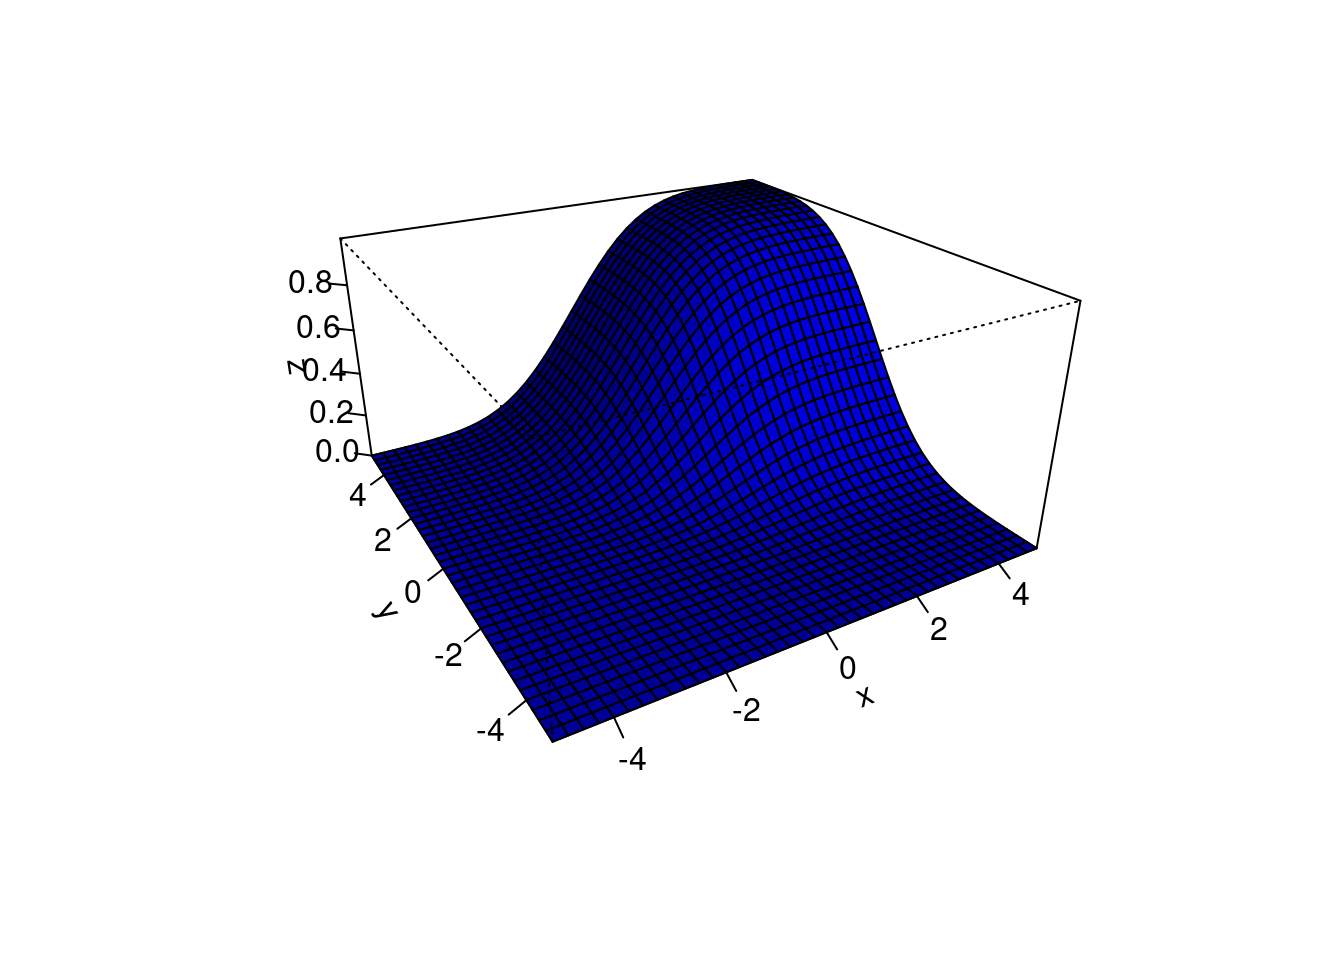
\includegraphics[width=0.8\linewidth]{figure/minimal-unnamed-chunk-37-1} \end{center}

\hypertarget{multidimensional-probability-function}{%
\subsubsection{Multidimensional Probability Function}\label{multidimensional-probability-function}}

\paragraph*{Discrete random vectors.}

\(X\) takes only countably many (i.e.~discrete) values \(\mathbf{x}_1,\mathbf{x}_2,\dots\in\mathbb{R}^d\) and has a \textbf{multidimensional probability function} \(p(\mathbf{x}_i)=P(X=\mathbf{x}_i)\) for \(i=1,2,\dots\). That is,
\begin{align*}
P(X\in [a_1,b_1]\times\dots\times [a_d,b_d])=
\sum_{\mathbf{x}_i\in [a_1,b_1]\times\dots\times [a_d,b_d]}p(\mathbf{x}_i).
\end{align*}

\hypertarget{multidimensional-density-function}{%
\subsubsection{Multidimensional Density Function}\label{multidimensional-density-function}}

\paragraph*{Continouse random vectors.}

\(X\) takes values in \(\mathbb{R}^d\) and has a \textbf{multidimensional density function} \(f(x_1,\dots,x_d)\). That is,
\begin{align*}
P(X\in [a_1,b_1]\times\dots\times [a_d,b_d])=\int\limits_{a_d}^{b_d}\dots \int\limits _{a_1}^{b_1}f(x_1,\dots,x_d)dx_1\dots dx_d.
\end{align*}
In the following we focus only on continuous random vectors -- the discrete cases are treated analogously. Properties of \textbf{multivariate density} functions:

\begin{itemize}
\item $\displaystyle f(x_1,\dots,x_d)\geq 0$\par\noindent
\item $\displaystyle \int_{-\infty}^{\infty}\dots \int_{-\infty}^{\infty}f(x_1,\dots,x_d)dx_1\dots dx_d=1$
\end{itemize}

\begin{Shaded}
\begin{Highlighting}[]
\DocumentationTok{\#\# Load the package}
\FunctionTok{library}\NormalTok{(mnormt)}

\NormalTok{x     }\OtherTok{\textless{}{-}} \FunctionTok{seq}\NormalTok{(}\SpecialCharTok{{-}}\DecValTok{5}\NormalTok{, }\DecValTok{5}\NormalTok{, }\FloatTok{0.25}\NormalTok{) }
\NormalTok{y     }\OtherTok{\textless{}{-}} \FunctionTok{seq}\NormalTok{(}\SpecialCharTok{{-}}\DecValTok{5}\NormalTok{, }\DecValTok{5}\NormalTok{, }\FloatTok{0.25}\NormalTok{)}
\NormalTok{mu    }\OtherTok{\textless{}{-}} \FunctionTok{c}\NormalTok{(}\DecValTok{0}\NormalTok{, }\DecValTok{0}\NormalTok{)}
\NormalTok{sigma }\OtherTok{\textless{}{-}} \FunctionTok{matrix}\NormalTok{(}\FunctionTok{c}\NormalTok{(}\DecValTok{2}\NormalTok{, }\SpecialCharTok{{-}}\DecValTok{1}\NormalTok{, }\SpecialCharTok{{-}}\DecValTok{1}\NormalTok{, }\DecValTok{2}\NormalTok{), }\AttributeTok{nrow =} \DecValTok{2}\NormalTok{)}
\NormalTok{f     }\OtherTok{\textless{}{-}} \ControlFlowTok{function}\NormalTok{(x, y) }\FunctionTok{dmnorm}\NormalTok{(}\FunctionTok{cbind}\NormalTok{(x, y), mu, sigma)}
\NormalTok{z     }\OtherTok{\textless{}{-}} \FunctionTok{outer}\NormalTok{(x, y, f)}

\FunctionTok{persp}\NormalTok{(x, y, z, }\AttributeTok{theta =} \SpecialCharTok{{-}}\DecValTok{30}\NormalTok{, }\AttributeTok{phi =} \DecValTok{25}\NormalTok{, }
      \AttributeTok{shade =} \FloatTok{0.75}\NormalTok{, }\AttributeTok{col =} \StringTok{"blue"}\NormalTok{, }\AttributeTok{expand =} \FloatTok{0.5}\NormalTok{, }\AttributeTok{r =} \DecValTok{2}\NormalTok{, }
      \AttributeTok{ltheta =} \DecValTok{25}\NormalTok{, }\AttributeTok{ticktype =} \StringTok{"detailed"}\NormalTok{)}
\end{Highlighting}
\end{Shaded}

\begin{center}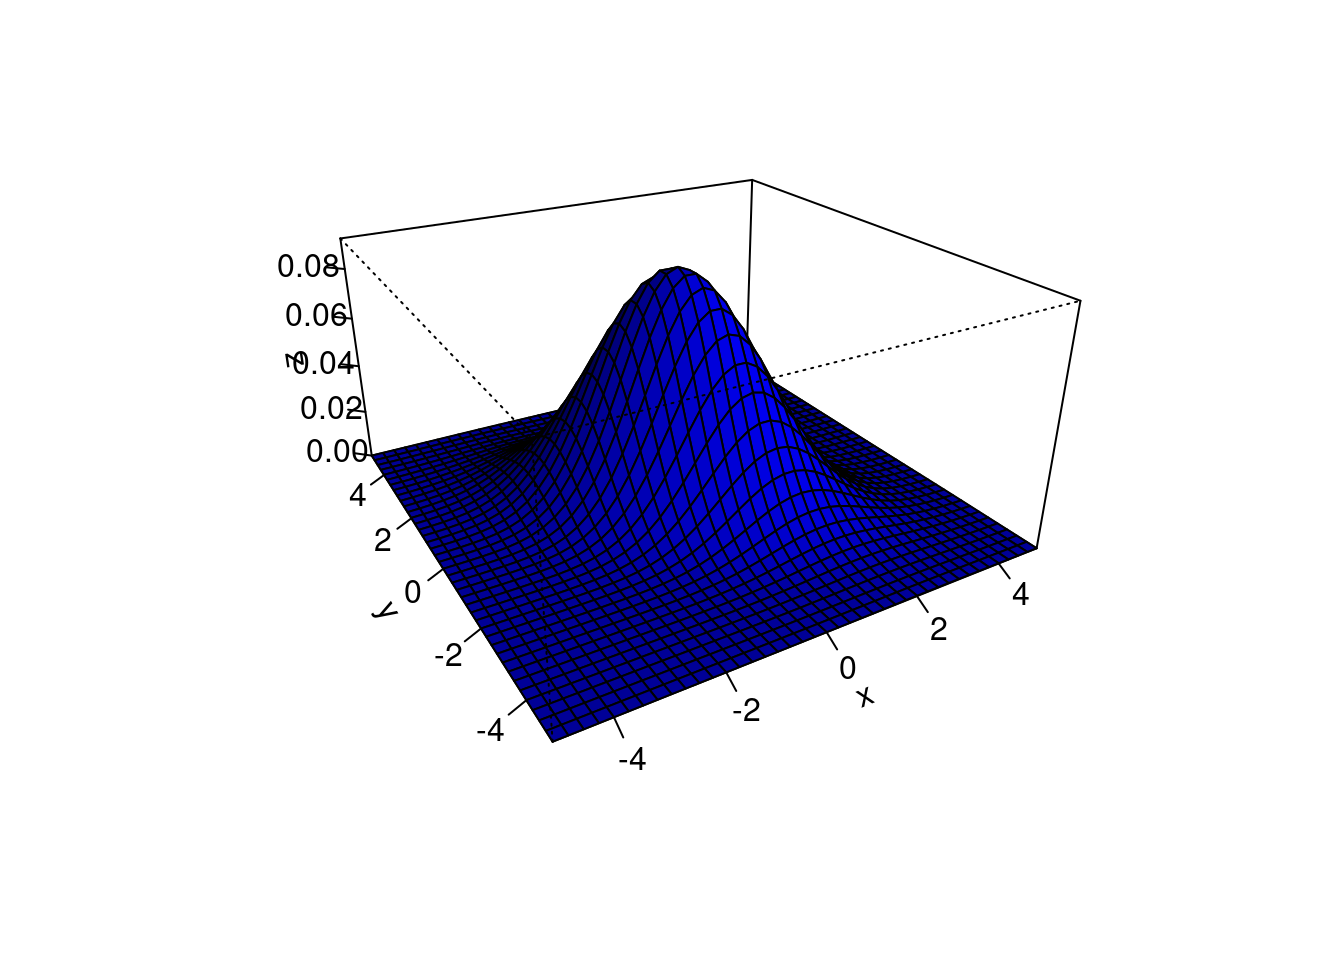
\includegraphics[width=0.8\linewidth]{figure/minimal-unnamed-chunk-38-1} \end{center}

\hypertarget{marginal-distribution-and-density-functions}{%
\subsubsection{Marginal Distribution and Density Functions}\label{marginal-distribution-and-density-functions}}

Each random element, \(X_j\), with \(j=1,\dots,d\), of the random vector \(X\) has its own \textbf{marginal distribution} \(F_j\). This is just the univariate distribution of \(X_j\) when ignoring all other random variables in \(X\). Formally we have:

\begin{itemize}
\item \textbf{Marginal distribution function:} $F_j(x)=P(X_j\leq x)$
\item \textbf{Marginal density function:} $f_j$, for instance, for $j=1$:
$$f_1({\color{blue}x_1})=\int_{-\infty}^{\infty}\dots \int_{-\infty}^{\infty}f({\color{blue}x_1},x_2\dots,
x_d)dx_2\dots  dx_d$$
\end{itemize}

\begin{center}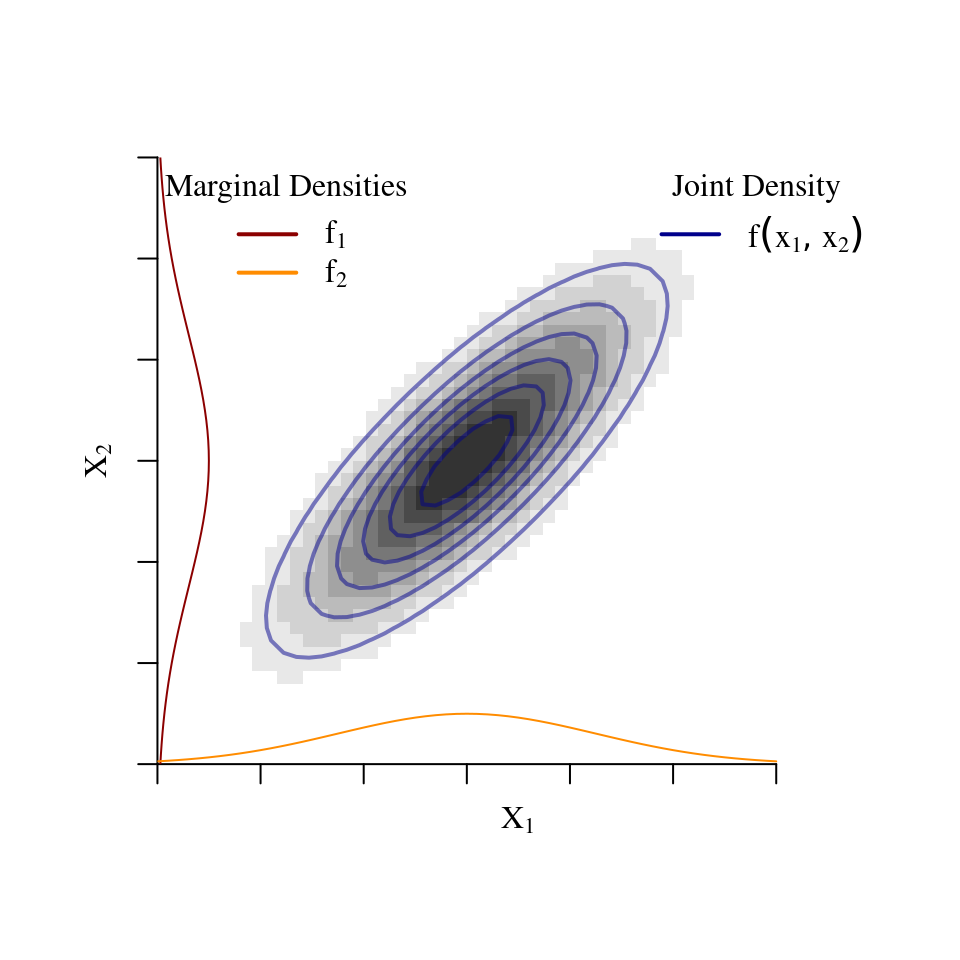
\includegraphics[width=0.8\linewidth]{figure/minimal-unnamed-chunk-39-1} \end{center}

\hypertarget{condDistr}{%
\subsubsection{Conditional Distributions}\label{condDistr}}

Often, we are interested in the \textbf{conditional distribution} of \(X_j\) given certain values of all other random variables\\
\[X_1=x_1,\ldots, X_{j-1}=x_{j-1}, X_{j+1}=x_{j+1},\ldots,X_d=x_d.\]
That is, the distribution of \(X_j\) when fixing the values of\\
\(X_1=x_1,\ldots,\) \(X_{j-1}=x_{j-1},\) \(X_{j+1}=x_{j+1},\ldots, X_d=x_d\). An important tool is here the \textbf{conditional density} of, for instance, \(X_1\) given \(X_2=x_2,\ldots,X_d=x_d\):
\[
f(x_1\mid x_2,\ldots,x_d)=\frac{f(x_1,x_2,\ldots,x_d)}{f_{X_{2},\ldots,X_{d}}(x_2,\ldots,x_d)},
\]
where \(f_{X_{2},\ldots,X_{d}}\) denotes the joint density of \(X_2,\ldots,X_d\).

\begin{center}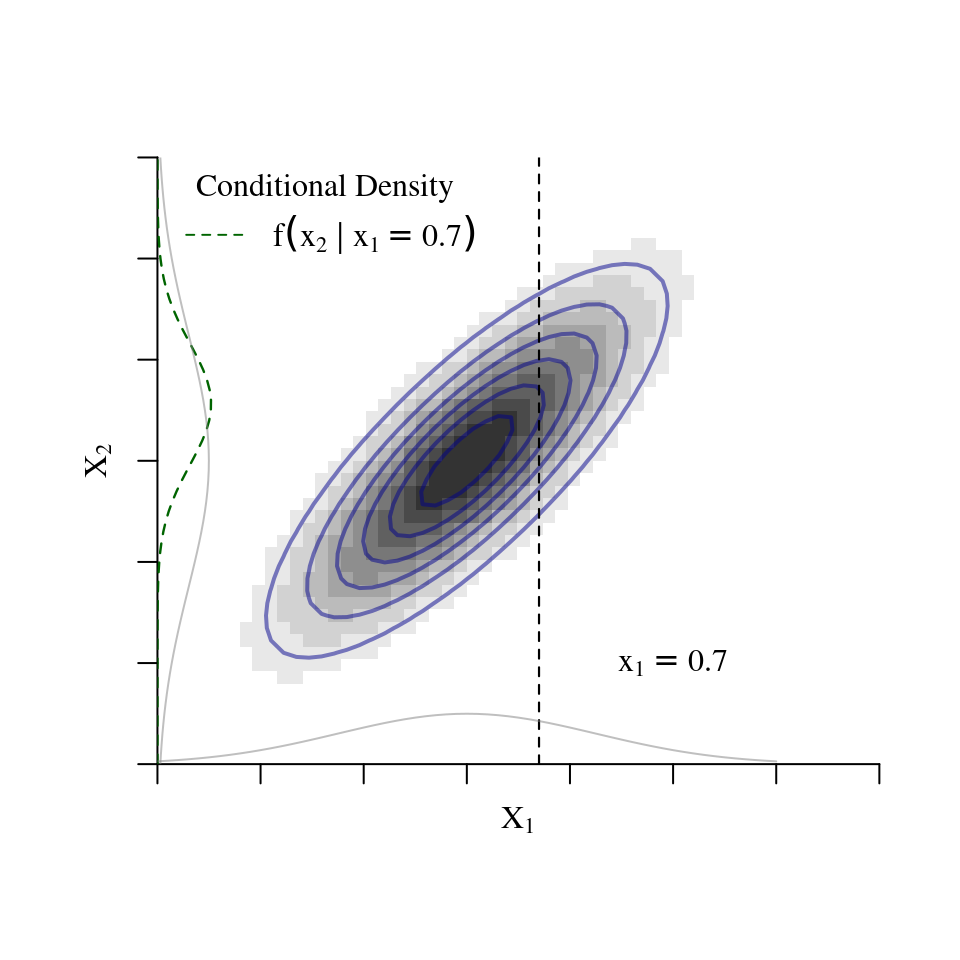
\includegraphics[width=0.8\linewidth]{figure/minimal-unnamed-chunk-40-1} \end{center}

\hypertarget{means-and-moments}{%
\subsection{Means and Moments}\label{means-and-moments}}

\hypertarget{unconditional-means}{%
\subsection{Unconditional Means}\label{unconditional-means}}

The \textbf{unconditional mean} of \(X_1\) is given by
\[
E(X_1)= \int x f_{X_1}(x)dx.
\]
The unconditional mean of a random vector \(X=(X_1,\dots,X_d)'\) is given by the vector of element-wise means
\[
E(X)=(E(X_1),\dots,E(X_d))'.
\]

\hypertarget{conditional-means}{%
\subsection{Conditional Means}\label{conditional-means}}

Of central importance in \textbf{regression analysis} is the \textbf{conditional mean}. The conditional mean of \(X_1\) for given values \(X_2=x_2,\ldots,X_d=x_d\):
\begin{align*}
  m(x_2,\dots,x_d):&=E(X_1|X_2=x_2,\ldots,X_d=x_d)\\
                   &= \int x_1 f(x_1\mid x_2,\ldots,x_d)dx_1,
\end{align*}\\
where \(m(x_2,\dots,x_d)\) denotes the \textbf{regression function}.

\hypertarget{means-of-transformed-random-variables-and-moments}{%
\subsection{Means of Transformed Random Variables and Moments}\label{means-of-transformed-random-variables-and-moments}}

The \textbf{mean of a transformed random variable} \(r(X)\) is given by
\[
E(r(X))=\int r(x) f_{X}(x)dx.
\]
Typical transformations are, for instance

\begin{itemize}
\item centering $r(x)=x-E(X)$,
\item centering and scaling $r(x)=(x-E(X))/\sqrt{Var(X)}$, 
\item or $r(x)=(x - E(X))^2$, 
\end{itemize}

where the latter transformation leads to the \textbf{second central moment}, i.e.~the variance of \(X\), \(Var(X)=\int (x - E(X))^2 f_{X}(x)dx\).

\bigskip

\begin{itemize}
\item
  The k\(th\), \(k>0\), moment is given by
  \[
  \mu_{k}=\mathrm{E}\left[X^{k}\right]=\int_{-\infty}^{+\infty}x^{k} f_X(x)d x.
  \]
\item
  The k\(th\), \(k>1\), central moment is given by
  \[
  \mu^c_{k}=\mathrm{E}\left[(X-\mathrm{E}[X])^{k}\right]=\int_{-\infty}^{+\infty}(x-\mu)^{k} f_X(x)d x,
  \]
  where \(\mu=E(X)\).
\end{itemize}

\paragraph*{Note.}

Moments determine the tail of a distribution (but not much else); see \cite{LB2000}. Roughly: The more moments a distribution has the faster converge its tails to zero. Distributions with compact supports (e.g.~the uniform distribution \(U[a,b]\)) have infinitely many moments. The Normal distribution has also infinitely many moments -- even though this distribution has not a compact support since \(\phi(x)>0\) for all \(x\in\mathbb{R}\). .

\hypertarget{law-of-total-expectation}{%
\subsubsection{Law of Total Expectation}\label{law-of-total-expectation}}

As long as we do not fix the values of the conditioning variables, \(X_2,\dots,X_d\), they are random variables. Consequently, the conditional mean is generally itself a random variable
\[
E(X_1|X_2,\ldots,X_d)=\int x_1 f(x_1\mid X_2,\ldots,X_d)dx_1. 
\]
Note that \(f(x_1\mid X_2,\ldots,X_d)\) is just a transformation of the random variables \(X_2,\dots,X_d\). So we can easily compute the unconditional mean \(E(X_1)\) by taking the mean of \(E(X_1|X_2,\ldots,X_d)\) as following,
\begin{align*}
&E\big({\color{RedViolet}E(X_1|X_2,\ldots,X_d)}\big)=\\
&=\int\dots\int\;{\color{RedViolet}\int x_1 f(x_1\mid x_2,\ldots,x_d)dx_1}\;f_{X_2,\dots,X_d}(x_2,\ldots,x_d)dx_2\dots dx_d\\
&=\int x_1 \left(\int\dots\int f(x_1,{\color{blue}x_2,\ldots,x_d}){\color{blue}dx_2\dots dx_d}\right)dx_1\\
&=\int x_1 f_{X_1}(x_1)dx_1\\
&=E(X_1).
\end{align*}

The result that \(E\big(E(X_1|X_2,\ldots,X_d)\big)=E(X_1)\) is called \textbf{law of total expectation} or \textbf{law of iterated expectation}.

\hypertarget{independent-random-variables}{%
\subsection{Independent Random Variables}\label{independent-random-variables}}

Random variables \(X_1,\dots,X_d\) are mutually \textbf{independent} if for all \(x=(x_1,\dots,x_d)^\prime\) it is true that
\begin{align*}
  F(x_1,\dots,x_d)&=F_1(x_1)\cdot F_2(x_2)\cdot\ldots\cdot F_d(x_d)\\
  f(x_1,\dots,x_d)&=f_1(x_1)\cdot f_2(x_2)\cdot\ldots\cdot f_d(x_d)
\end{align*}

\noindent The following holds true:

\begin{itemize}
\item  Two real-valued random variables $X$ and $Y$ are independent from each other \textit{if and only if} the marginal density of $X$ equals the conditional density of $X$ given $Y=y$ for all $y\in\mathbb{R}$,
$$f_X(x)=f_{X|Y}(x\mid y)\quad \text{ for all } y\in\mathbb{R}.$$
Of course, the same statement applies to the marginal density of $Y$ given $X=x$ for all $x\in\mathbb{R}$. That is, $X$ and $Y$ are two independent real-valued random variables \textit{if and only if} 
$f_Y(y)=f_{Y|X}(y\mid x)$ for all $x\in\mathbb{R}.$
\item  If a real-valued random variable $X$ is independent from a real-valued random variable $Y$, then the conditional mean of $X$ given $Y=y$ equals the unconditional mean of $X$ for all $y\in\mathbb{R}$ (i.e. the regression function becomes a constant)
$$E(X\mid Y=y)=E(X)\quad \text{ for all } y\in\mathbb{R}.$$
Of course, the same statement applies to the conditional mean of $Y$ given $X=x$ for all $x\in\mathbb{R}$; i.e., if $X$ and $Y$ are two independent random variables, then 
$E(Y\mid X=x)=E(Y)\quad \text{ for all } x\in\mathbb{R}.$\newline
\paragraph*{Cautionary note.} The properties that $E(X\mid Y=y)=E(X)$ for all $y\in\mathbb{R}$ or that $E(Y\mid X=x)=E(Y)$ for all $x\in\mathbb{R}$, do \textbf{not} imply that $Y$ and $X$ are independent. 
\end{itemize}

\hypertarget{i.i.d.-samples}{%
\subsection{I.I.D. Samples}\label{i.i.d.-samples}}

Tradition dictates that the sample size is denoted by the natural number \(n\in\{1,2,\dots\}\). A random sample is a collection \(X=(X_{1}, \ldots, X_{n})\) of random variables \(X_{1}, \ldots, X_{n}\). If \(X_{1}, \ldots, X_{n}\) are all \textbf{independent} from each other and if each random variable has the same marginal distribution, we say that the random sample
\[
X=(X_{1}, \ldots, X_{n})\text{ is \textbf{i.i.d. (independent and identically distributed)}}. 
\]

\hypertarget{some-important-discrete-random-variables}{%
\subsection{Some Important Discrete Random Variables}\label{some-important-discrete-random-variables}}

\hypertarget{the-discrete-uniform-distribution}{%
\subsubsection{The Discrete Uniform Distribution}\label{the-discrete-uniform-distribution}}

Let \(k>1\) be a given integer. Suppose that \(X\) has probability mass function given by
\[
f(x)=\left\{\begin{array}{ll}
1 / k & \text { for } x=1, \ldots, k \\
0 & \text { otherwise. }
\end{array}\right.
\]
We say that \(X\) has a uniform distribution on \(\{1, \ldots, k\}\).

\begin{Shaded}
\begin{Highlighting}[]
\FunctionTok{set.seed}\NormalTok{(}\DecValTok{51}\NormalTok{)}
\DocumentationTok{\#\# Set the parameter k}
\NormalTok{k }\OtherTok{\textless{}{-}} \DecValTok{10}
\DocumentationTok{\#\# Draw one realization from the discrete uniform distribution}
\FunctionTok{sample}\NormalTok{(}\AttributeTok{x =} \DecValTok{1}\SpecialCharTok{:}\NormalTok{k, }\AttributeTok{size =} \DecValTok{1}\NormalTok{, }\AttributeTok{replace =} \ConstantTok{TRUE}\NormalTok{)}
\CommentTok{\#\textgreater{} [1] 7}
\end{Highlighting}
\end{Shaded}

\hypertarget{the-bernoulli-distribution}{%
\subsubsection{The Bernoulli Distribution}\label{the-bernoulli-distribution}}

Let \(X\) represent a possibly unfair coin flip. Then \(P(X=1)=p\) and \(P(X=0)=1-p\) for some \(p \in[0,1]\). We say that \(X\) has a Bernoulli distribution written \(X\sim\operatorname{Bernoulli }(p)\). The probability function is \(f(x)=p^{x}(1-p)^{1-x}\) for \(x \in\{0,1\}\)

\begin{Shaded}
\begin{Highlighting}[]
\FunctionTok{set.seed}\NormalTok{(}\DecValTok{51}\NormalTok{)}
\DocumentationTok{\#\# Set the parameter p}
\NormalTok{p }\OtherTok{\textless{}{-}} \FloatTok{0.25}
\DocumentationTok{\#\# Draw n realization from the discrete uniform distribution}
\NormalTok{n }\OtherTok{\textless{}{-}} \DecValTok{5}
\FunctionTok{sample}\NormalTok{(}\AttributeTok{x =} \FunctionTok{c}\NormalTok{(}\DecValTok{0}\NormalTok{,}\DecValTok{1}\NormalTok{), }\AttributeTok{size =}\NormalTok{ n, }\AttributeTok{prob =} \FunctionTok{c}\NormalTok{(}\DecValTok{1}\SpecialCharTok{{-}}\NormalTok{p, p), }\AttributeTok{replace=}\ConstantTok{TRUE}\NormalTok{)}
\CommentTok{\#\textgreater{} [1] 1 0 0 1 0}

\DocumentationTok{\#\# Alternatively:}
\DocumentationTok{\#\# (Bernoulli(p) equals Binomial(1,p))}
\FunctionTok{rbinom}\NormalTok{(}\AttributeTok{n =}\NormalTok{ n, }\AttributeTok{size =} \DecValTok{1}\NormalTok{, }\AttributeTok{prob =}\NormalTok{ p)}
\CommentTok{\#\textgreater{} [1] 1 1 0 1 0}
\end{Highlighting}
\end{Shaded}

\hypertarget{the-binomial-distribution}{%
\subsubsection{The Binomial Distribution}\label{the-binomial-distribution}}

Suppose we have a coin which falls heads with probability \(p\) for some \(p\in[0,1]\). Flip the coin \(n\) times and let \(X\) be the number of heads (or successes). Assume that the tosses are independent. Let \(f(x)=P(X=x)\) be the mass function. It can be shown that
\[
f(x)=\left\{
\begin{array}{ll}
\left(\begin{array}{l}
n \\
x
\end{array}\right) p^{x}(1-p)^{n-x} & \text { for } x=0, \ldots, n \\
0 & \text { otherwise. }
\end{array}\right.
\]
A random variable with this mas function is called a \textbf{binomial random variable} and we write \(X \sim \operatorname{Binomial}(n, p)\). If \(X_{1} \sim\) Binomial \(\left(n_1, p1\right)\) and \(X_{2} \sim\) Binomial\(\left(n_2, p\right)\) and if \(X_1\) and \(X_2\) are independent, then \(X_{1}+X_{2} \sim \operatorname{Binomial}\left(n_1+n_2, p\right)\)

\begin{Shaded}
\begin{Highlighting}[]
\FunctionTok{set.seed}\NormalTok{(}\DecValTok{51}\NormalTok{)}
\DocumentationTok{\#\# Set the parameters n and p}
\NormalTok{size }\OtherTok{\textless{}{-}}   \DecValTok{10} \CommentTok{\# number of trials}
\NormalTok{p    }\OtherTok{\textless{}{-}} \FloatTok{0.25} \CommentTok{\# prob of success}

\DocumentationTok{\#\# Draw n realization from the binomial distribution:}
\NormalTok{n }\OtherTok{\textless{}{-}} \DecValTok{5}
\FunctionTok{rbinom}\NormalTok{(}\AttributeTok{n =}\NormalTok{ n, }\AttributeTok{size =}\NormalTok{ size, }\AttributeTok{prob =}\NormalTok{ p)}
\CommentTok{\#\textgreater{} [1] 4 1 2 6 1}
\end{Highlighting}
\end{Shaded}

\hypertarget{some-important-continuous-random-variables}{%
\subsection{Some Important Continuous Random Variables}\label{some-important-continuous-random-variables}}

\hypertarget{the-uniform-distribution}{%
\subsubsection{The Uniform Distribution}\label{the-uniform-distribution}}

\(X\) has a \(\operatorname{Uniform}(a, b)\) distribution, written \(X\sim \operatorname{Uniform}(a, b),\) if
\[
f(x)=\left\{\begin{array}{ll}
\frac{1}{b-a} & \text { for } x \in[a, b] \\
0 & \text { otherwise }
\end{array}\right.
\]
where \(a<b\). The distribution function is
\[
F(x)=\left\{\begin{array}{ll}
0 & x<a \\
\frac{x-a}{b-a} & x \in[a, b] \\
1 & x>b
\end{array}\right.
\]

\begin{Shaded}
\begin{Highlighting}[]
\DocumentationTok{\#\# Drawing from the uniform distribution:}
\NormalTok{n }\OtherTok{\textless{}{-}} \DecValTok{10}
\NormalTok{a }\OtherTok{\textless{}{-}} \DecValTok{0}
\NormalTok{b }\OtherTok{\textless{}{-}} \DecValTok{1}
\FunctionTok{runif}\NormalTok{(}\AttributeTok{n =}\NormalTok{ n, }\AttributeTok{min =}\NormalTok{ a, }\AttributeTok{max =}\NormalTok{ b)}
\CommentTok{\#\textgreater{}  [1] 0.83442365 0.75138318 0.40601047 0.97101998 0.11233151 0.50750617 0.69714201}
\CommentTok{\#\textgreater{}  [8] 0.17104008 0.25448233 0.01813812}
\end{Highlighting}
\end{Shaded}

\hypertarget{the-normal-or-gaussian-distribution}{%
\subsubsection{The Normal (or Gaussian) Distribution}\label{the-normal-or-gaussian-distribution}}

\(X\) has a Normal (or Gaussian) distribution with parameters \(\mu\) and \(\sigma,\) denoted by \(X \sim N\left(\mu, \sigma^{2}\right),\) if
\[
f(x)=\frac{1}{\sigma \sqrt{2 \pi}} \exp \left\{-\frac{1}{2 \sigma^{2}}(x-\mu)^{2}\right\}, \quad x \in \mathbb{R}
\]
where \(\mu \in \mathbb{R}\) and \(\sigma>0.\) Later we shall see that \(\mu\) is the \say{center} (or mean of the distribution and \(\sigma\) is the \say{spread} (or standard deviation) of the distribution. The Normal plays an important role in probability and statistics. Many phenomena in nature have approximately Normal distributions. The \textbf{Central Limit Theorem} gives a special role to the Normal distribution by stating that the distribution of averages of random variables can be approximated by a Normal distribution.

We say that \(X\) has a standard Normal distribution if \(\mu=0\) and \(\sigma=1\). Tradition dictates that a standard Normal random variable is denoted by \(Z\). The PDF and CDF of a standard Normal are denoted by \(\phi(z)\) and \(\Phi(z)\). There is no closed-form expression for \(\Phi\). Here are some useful facts:

\begin{enumerate}
\def\labelenumi{(\roman{enumi})}
\item
  If \(X \sim N\left(\mu, \sigma^{2}\right)\) then \(Z=(X-\mu) / \sigma \sim N(0,1)\)
\item
  If \(Z \sim N(0,1)\) then \(X=\mu+\sigma Z \sim N\left(\mu, \sigma^{2}\right)\)
\item
  If \(X_{i} \sim N\left(\mu_{i}, \sigma_{i}^{2}\right), i=1, \ldots, n\) are independent then
  \[
  \sum_{i=1}^{n} X_{i} \sim N\left(\sum_{i=1}^{n} \mu_{i}, \sum_{i=1}^{n} \sigma_{i}^{2}\right).
  \]
\end{enumerate}

The following \textsf{R}-codes plots the standard Normal density function:

\begin{Shaded}
\begin{Highlighting}[]
\CommentTok{\# draw a plot of the N(0,1) PDF}
\FunctionTok{curve}\NormalTok{(}\FunctionTok{dnorm}\NormalTok{(x),}
      \AttributeTok{xlim =} \FunctionTok{c}\NormalTok{(}\SpecialCharTok{{-}}\FloatTok{3.5}\NormalTok{, }\FloatTok{3.5}\NormalTok{),}
      \AttributeTok{ylab =} \StringTok{"Density"}\NormalTok{, }
      \AttributeTok{main =} \StringTok{"Standard Normal Density Function"}\NormalTok{) }
\end{Highlighting}
\end{Shaded}

\begin{center}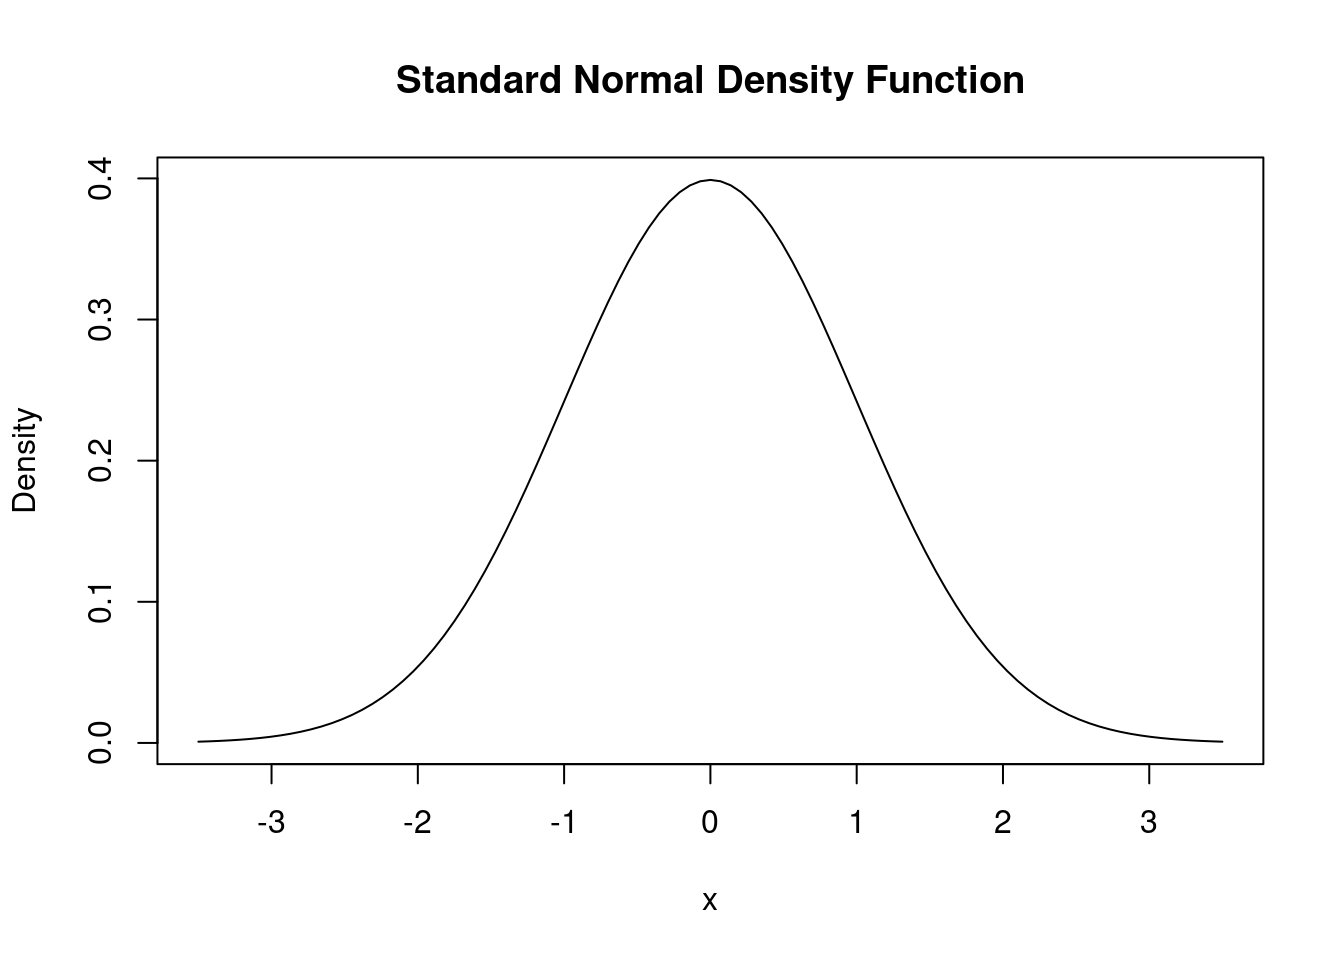
\includegraphics[width=0.8\linewidth]{figure/minimal-unnamed-chunk-45-1} \end{center}

This is how you can draw realizations from pseudo random Normal variables:

\begin{Shaded}
\begin{Highlighting}[]
\DocumentationTok{\#\# Drawing from the uniform distribution:}
\NormalTok{n     }\OtherTok{\textless{}{-}} \DecValTok{12}
\NormalTok{mu    }\OtherTok{\textless{}{-}} \DecValTok{0}
\NormalTok{sigma }\OtherTok{\textless{}{-}} \DecValTok{1}
\FunctionTok{rnorm}\NormalTok{(}\AttributeTok{n =}\NormalTok{ n, }\AttributeTok{mean =}\NormalTok{ mu, }\AttributeTok{sd =}\NormalTok{ sigma) }
\CommentTok{\#\textgreater{}  [1]  0.085602504 {-}0.695791615 {-}1.364410561 {-}0.183503290 {-}1.675347076  0.007303551}
\CommentTok{\#\textgreater{}  [7]  0.346965187  0.037914318  0.881345676 {-}0.882815597 {-}0.883560071 {-}0.795629557}
\end{Highlighting}
\end{Shaded}

An extension of the normal distribution in a univariate setting is the multivariate normal distribution. Let \(X=(X_1,\dots,X_k)'\) be a \(k\)-dimensional normal variable, short \(X\sim N_k(\mu,\Sigma)\) with mean vector \(E(X)=\mu\in\mathbb{R}^k\) and covariance matrix \(\operatorname{Cov}(X)=\Sigma\). The joint density function or \textbf{probability density function (pdf)} of the \(k\)-dimensional multivariate normal distribution is
\[
f_{X}\left(x_{1}, \ldots, x_{k}\right)=\frac{\exp \left(-\frac{1}{2}(x-\mu)' \Sigma^{-1}(x-\mu)\right)}{\sqrt{(2 \pi)^{k}|\Sigma|}},
\]
where \(|\Sigma|\) denotes the determinant of \(\Sigma\). For \(k=2\) we have the bivariate pdf of two random normal variables, \(X\) and \(Y\) say
\begin{align*}
g_{X,Y}(x,y) =& \, \frac{1}{2\pi\sigma_X\sigma_Y\sqrt{1-\rho_{XY}^2}} \\ 
\cdot & \, \exp \left\{ \frac{1}{-2(1-\rho_{XY}^2)} \left[ \left( \frac{x-\mu_x}{\sigma_X} \right)^2 - 2\rho_{XY}\left( \frac{x-\mu_X}{\sigma_X} \right)\left( \frac{y-\mu_Y}{\sigma_Y} \right) + \left( \frac{y-\mu_Y}{\sigma_Y} \right)^2 \right]  \right\}.
\end{align*}
Lets consider the special case where \(X\) and \(Y\) are independent standard normal random variables with densities \(f_X(x)\) and \(f_Y(y)\). We then have the parameters \(\sigma_X = \sigma_Y = 1\), \(\mu_X=\mu_Y=0\) (due to marginal standard normality) and correlation \(\rho_{XY}=0\) (due to independence). The joint density of \(X\) and \(Y\) then becomes
\[
g_{X,Y}(x,y) = f_X(x) f_Y(y) = \frac{1}{2\pi} \cdot \exp \left\{ -\frac{1}{2}\left[x^2 + y^2\right]\right\}.
\]

\hypertarget{chisqdist}{%
\subsubsection{The Chi-Squared Distribution}\label{chisqdist}}

The chi-squared distribution is another distribution relevant in econometrics. It is often needed when testing special types of hypotheses frequently encountered when dealing with regression models.

The sum of \(M\) squared \emph{independent standard normal} distributed random variables, \(Z_1,\dots,Z_M\) follows a chi-squared distribution with \(M\) degrees of freedom:
\begin{align*}
Z_1^2 + \dots + Z_M^2 = \sum_{m=1}^M Z_m^2 \sim \chi^2_M. 
\end{align*}
A \(\chi^2\) distributed random variable with \(M\) degrees of freedom has expectation \(M\), mode at \(M-2\) for \(M \geq 2\) and variance \(2 \cdot M\).

Using the code below, we can display the pdf and the distribution function or \textbf{cumulated density function (cdf)} of a \(\chi^2_3\) random variable in a single plot. This is achieved by setting the argument \texttt{add\ =\ TRUE"} in the second call of \texttt{"curve()"}. Further we adjust limits of both axes using \texttt{"xlim"} and \texttt{"ylim"} and choose different colors to make both functions better distinguishable. The plot is completed by adding a legend with help of \texttt{"legend()"}.

\begin{Shaded}
\begin{Highlighting}[]
\CommentTok{\# plot the PDF}
\FunctionTok{curve}\NormalTok{(}\FunctionTok{dchisq}\NormalTok{(x, }\AttributeTok{df =} \DecValTok{3}\NormalTok{), }
      \AttributeTok{xlim =} \FunctionTok{c}\NormalTok{(}\DecValTok{0}\NormalTok{, }\DecValTok{10}\NormalTok{), }
      \AttributeTok{ylim =} \FunctionTok{c}\NormalTok{(}\DecValTok{0}\NormalTok{, }\DecValTok{1}\NormalTok{), }
      \AttributeTok{col =} \StringTok{"blue"}\NormalTok{,}
      \AttributeTok{ylab =} \StringTok{""}\NormalTok{,}
      \AttributeTok{main =} \StringTok{"pdf and cdf of Chi{-}Squared Distribution, M = 3"}\NormalTok{)}

\CommentTok{\# add the CDF to the plot}
\FunctionTok{curve}\NormalTok{(}\FunctionTok{pchisq}\NormalTok{(x, }\AttributeTok{df =} \DecValTok{3}\NormalTok{), }
      \AttributeTok{xlim =} \FunctionTok{c}\NormalTok{(}\DecValTok{0}\NormalTok{, }\DecValTok{10}\NormalTok{), }
      \AttributeTok{add =} \ConstantTok{TRUE}\NormalTok{, }
      \AttributeTok{col =} \StringTok{"red"}\NormalTok{)}

\CommentTok{\# add a legend to the plot}
\FunctionTok{legend}\NormalTok{(}\StringTok{"topleft"}\NormalTok{, }
       \FunctionTok{c}\NormalTok{(}\StringTok{"PDF"}\NormalTok{, }\StringTok{"CDF"}\NormalTok{), }
       \AttributeTok{col =} \FunctionTok{c}\NormalTok{(}\StringTok{"blue"}\NormalTok{, }\StringTok{"red"}\NormalTok{), }
       \AttributeTok{lty =} \FunctionTok{c}\NormalTok{(}\DecValTok{1}\NormalTok{, }\DecValTok{1}\NormalTok{))}
\end{Highlighting}
\end{Shaded}

\begin{center}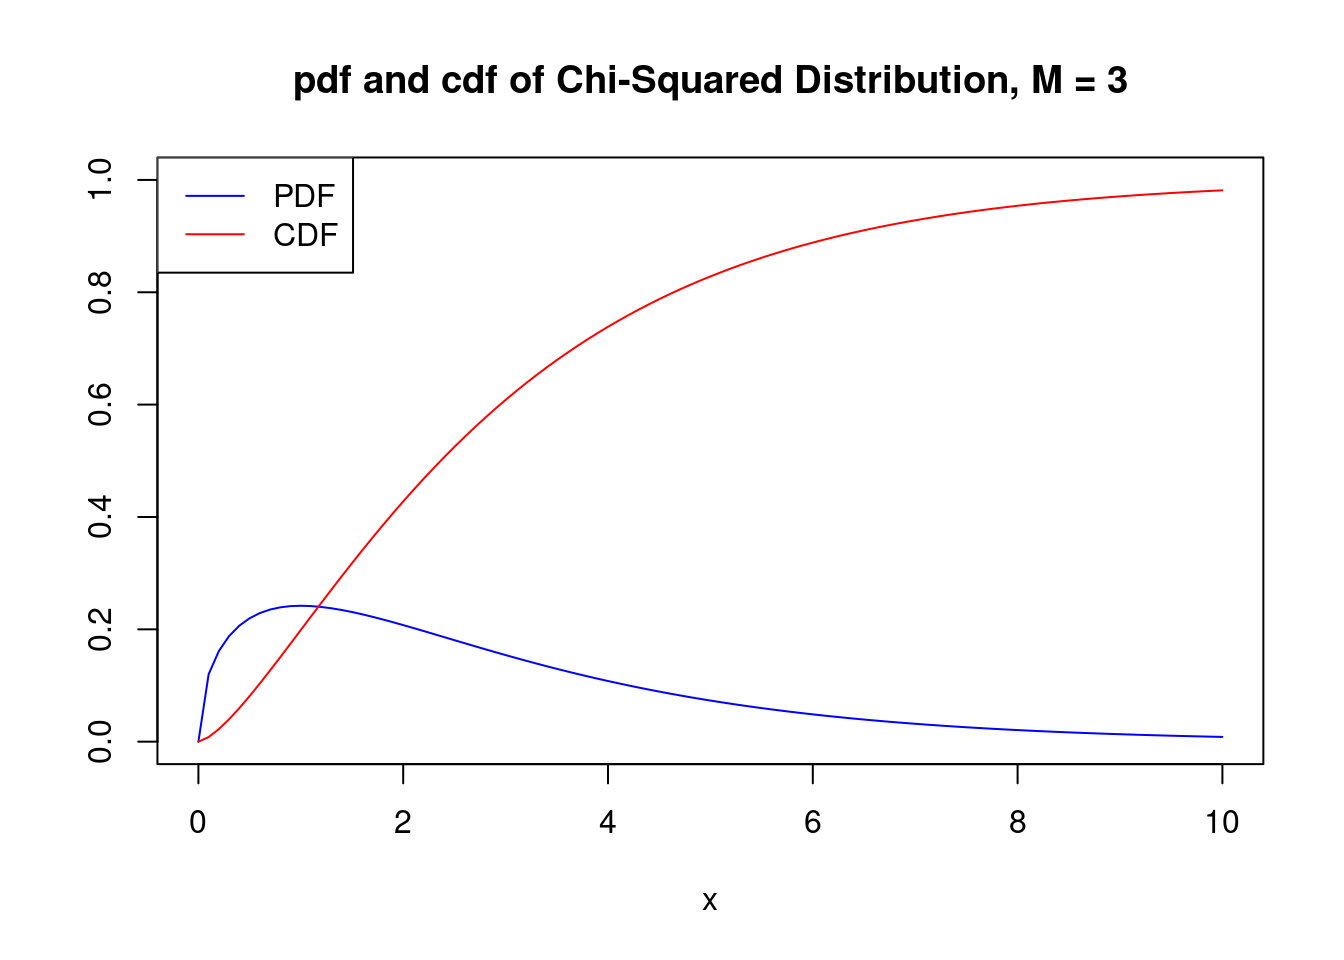
\includegraphics[width=0.8\linewidth]{figure/minimal-unnamed-chunk-47-1} \end{center}

Since the outcomes of a \(\chi^2_M\) distributed random variable are always positive, the support of the related PDF and CDF is \(\mathbb{R}_{\geq0}\).

As expectation and variance depend (solely!) on the degrees of freedom, the distribution's shape changes drastically if we vary the number of squared standard normals that are summed up. This relation is often depicted by overlaying densities for different \(M\), see the Wikipedia Article.

We reproduce this here by plotting the density of the \(\chi_1^2\) distribution on the interval \([0,15]\) with \texttt{"curve()"}. In the next step, we loop over degrees of freedom \(M=2,...,7\) and add a density curve for each \(M\) to the plot. We also adjust the line color for each iteration of the loop by setting \texttt{"col\ =\ M"}. At last, we add a legend that displays degrees of freedom and the associated colors.

\begin{Shaded}
\begin{Highlighting}[]
\CommentTok{\# plot the density for M=1}
\FunctionTok{curve}\NormalTok{(}\FunctionTok{dchisq}\NormalTok{(x, }\AttributeTok{df =} \DecValTok{1}\NormalTok{), }
      \AttributeTok{xlim =} \FunctionTok{c}\NormalTok{(}\DecValTok{0}\NormalTok{, }\DecValTok{15}\NormalTok{), }
      \AttributeTok{xlab =} \StringTok{"x"}\NormalTok{, }
      \AttributeTok{ylab =} \StringTok{"Density"}\NormalTok{, }
      \AttributeTok{main =} \StringTok{"Chi{-}Square Distributed Random Variables"}\NormalTok{)}

\CommentTok{\# add densities for M=2,...,7 to the plot using a \textquotesingle{}for()\textquotesingle{} loop }
\ControlFlowTok{for}\NormalTok{ (M }\ControlFlowTok{in} \DecValTok{2}\SpecialCharTok{:}\DecValTok{7}\NormalTok{) \{}
  \FunctionTok{curve}\NormalTok{(}\FunctionTok{dchisq}\NormalTok{(x, }\AttributeTok{df =}\NormalTok{ M),}
        \AttributeTok{xlim =} \FunctionTok{c}\NormalTok{(}\DecValTok{0}\NormalTok{, }\DecValTok{15}\NormalTok{), }
        \AttributeTok{add =}\NormalTok{ T, }
        \AttributeTok{col =}\NormalTok{ M)}
\NormalTok{\}}

\CommentTok{\# add a legend}
\FunctionTok{legend}\NormalTok{(}\StringTok{"topright"}\NormalTok{, }
       \FunctionTok{as.character}\NormalTok{(}\DecValTok{1}\SpecialCharTok{:}\DecValTok{7}\NormalTok{), }
       \AttributeTok{col =} \DecValTok{1}\SpecialCharTok{:}\DecValTok{7}\NormalTok{ , }
       \AttributeTok{lty =} \DecValTok{1}\NormalTok{, }
       \AttributeTok{title =} \StringTok{"D.F."}\NormalTok{)}
\end{Highlighting}
\end{Shaded}

\begin{center}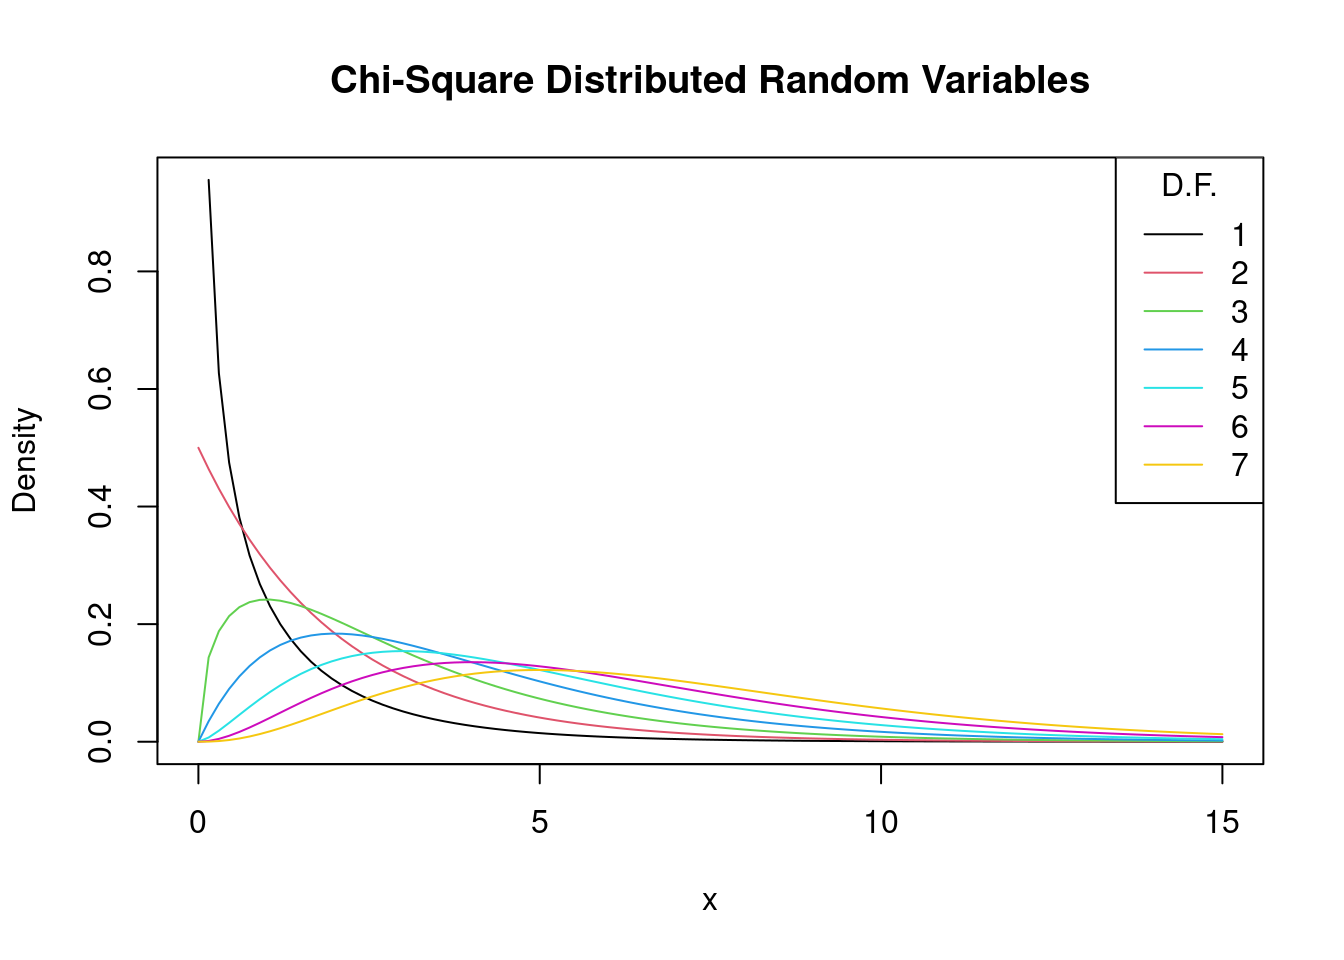
\includegraphics[width=0.8\linewidth]{figure/minimal-unnamed-chunk-48-1} \end{center}

Increasing the degrees of freedom shifts the distribution to the right (the mode becomes larger) and increases the dispersion (the distribution's variance grows).

\hypertarget{the-student-t-distribution}{%
\subsubsection{The Student t Distribution}\label{the-student-t-distribution}}

Let \(Z\) be a standard normal random variable, \(W\) a \(\chi^2_\nu\) random variable and further assume that \(Z\) and \(W\) are independent. Then it holds that
\[
\frac{Z}{\sqrt{W/\nu}} =:X \sim t_\nu
\]
and \(X\) follows a \emph{Student \(t\) distribution} (or simply \(t\) distribution) with \(\nu\) degrees of freedom.

The shape of a \(t_\nu\) distribution depends on \(\nu\). \(t\) distributions are symmetric, bell-shaped and look similar to a normal distribution, especially when \(\nu\) is large. This is not a coincidence: for a sufficiently large \(\nu\), the \(t_\nu\) distribution can be approximated by the standard normal distribution. This approximation works reasonably well for \(\nu\geq 30\).

A \(t_\nu\) distributed random variable \(X\) has an expectation if \(\nu>1\) and it has a variance if \(\nu>2\).
\begin{align*}
  E(X) =& 0, \ M>1 \\
  \text{Var}(X) =& \frac{M}{M-2}, \ M>2
\end{align*}

Let us plot some \(t\) distributions with different degrees of freedoms \(\nu\) and compare them to the standard normal distribution.

\begin{Shaded}
\begin{Highlighting}[]
\CommentTok{\# plot the standard normal density}
\FunctionTok{curve}\NormalTok{(}\FunctionTok{dnorm}\NormalTok{(x), }
      \AttributeTok{xlim =} \FunctionTok{c}\NormalTok{(}\SpecialCharTok{{-}}\DecValTok{4}\NormalTok{, }\DecValTok{4}\NormalTok{), }
      \AttributeTok{xlab =} \StringTok{"x"}\NormalTok{, }
      \AttributeTok{lty =} \DecValTok{2}\NormalTok{, }
      \AttributeTok{ylab =} \StringTok{"Density"}\NormalTok{, }
      \AttributeTok{main =} \StringTok{"Densities of t Distributions"}\NormalTok{)}

\CommentTok{\# plot the t density for M=2}
\FunctionTok{curve}\NormalTok{(}\FunctionTok{dt}\NormalTok{(x, }\AttributeTok{df =} \DecValTok{2}\NormalTok{), }
      \AttributeTok{xlim =} \FunctionTok{c}\NormalTok{(}\SpecialCharTok{{-}}\DecValTok{4}\NormalTok{, }\DecValTok{4}\NormalTok{), }
      \AttributeTok{col =} \DecValTok{2}\NormalTok{, }
      \AttributeTok{add =}\NormalTok{ T)}

\CommentTok{\# plot the t density for M=4}
\FunctionTok{curve}\NormalTok{(}\FunctionTok{dt}\NormalTok{(x, }\AttributeTok{df =} \DecValTok{4}\NormalTok{), }
      \AttributeTok{xlim =} \FunctionTok{c}\NormalTok{(}\SpecialCharTok{{-}}\DecValTok{4}\NormalTok{, }\DecValTok{4}\NormalTok{), }
      \AttributeTok{col =} \DecValTok{3}\NormalTok{, }
      \AttributeTok{add =}\NormalTok{ T)}

\CommentTok{\# plot the t density for M=25}
\FunctionTok{curve}\NormalTok{(}\FunctionTok{dt}\NormalTok{(x, }\AttributeTok{df =} \DecValTok{25}\NormalTok{), }
      \AttributeTok{xlim =} \FunctionTok{c}\NormalTok{(}\SpecialCharTok{{-}}\DecValTok{4}\NormalTok{, }\DecValTok{4}\NormalTok{), }
      \AttributeTok{col =} \DecValTok{4}\NormalTok{, }
      \AttributeTok{add =}\NormalTok{ T)}

\CommentTok{\# add a legend}
\FunctionTok{legend}\NormalTok{(}\StringTok{"topright"}\NormalTok{, }
       \FunctionTok{c}\NormalTok{(}\StringTok{"N(0, 1)"}\NormalTok{, }\StringTok{"M=2"}\NormalTok{, }\StringTok{"M=4"}\NormalTok{, }\StringTok{"M=25"}\NormalTok{), }
       \AttributeTok{col =} \DecValTok{1}\SpecialCharTok{:}\DecValTok{4}\NormalTok{, }
       \AttributeTok{lty =} \FunctionTok{c}\NormalTok{(}\DecValTok{2}\NormalTok{, }\DecValTok{1}\NormalTok{, }\DecValTok{1}\NormalTok{, }\DecValTok{1}\NormalTok{))}
\end{Highlighting}
\end{Shaded}

\begin{center}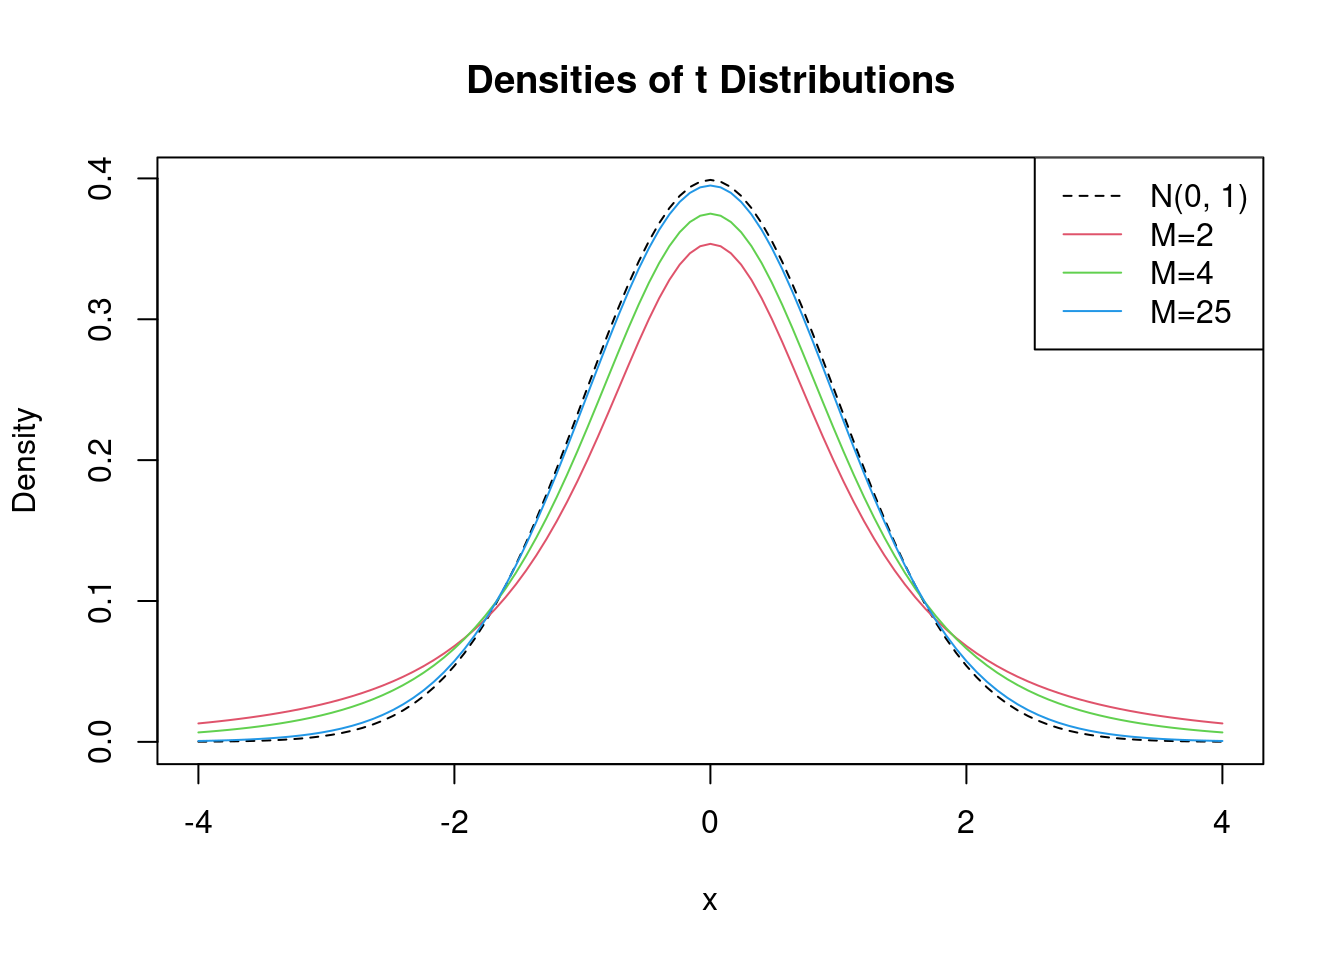
\includegraphics[width=0.8\linewidth]{figure/minimal-unnamed-chunk-49-1} \end{center}

The plot illustrates that as the degrees of freedom increase, the shape of the \(t\) distribution comes closer to that of a standard normal bell curve. Already for \(\nu=25\) we find little difference to the standard normal density. If \(\nu\) is small, we find the distribution to have heavier tails than a standard normal.

\hypertarget{cauchy-distribution}{%
\subsubsection{Cauchy Distribution}\label{cauchy-distribution}}

The Cauchy distribution is a special
case of the \(t\) distribution corresponding to \(\nu=1\). The density is
\[
f(x)=\frac{1}{\pi\left(1+x^{2}\right)}.
\]

For the Cauchy distribution, the \textbf{expectation does not exist} -- that is, it has no mean. Let's try to compute the mean of a Cauchy distribution and see what goes wrong. Its mean should be
\[
\mu=E(X)=\int_{-\infty}^{\infty} \frac{x d x}{\pi\left(1+x^{2}\right)}.
\]
In order for this improper integral to exist, we need both integrals \(\int_{-\infty}^{0}\) and \(\int_{0}^{\infty}\) to be finite. Let's look at the second integral.
\[
\int_{0}^{\infty} \frac{x d x}{\pi\left(1+x^{2}\right)}=\left.\frac{1}{2 \pi} \log \left(1+x^{2}\right)\right|_{0} ^{\infty}=\infty
\]
Similarly, the other integral, \(\int_{-\infty}^{0},\) is \(-\infty\). Since they're not both finite, the integral \(\int_{-\infty}^{\infty}\) doesn't exist. In other words \(\infty-\infty\) is not a number. Thus, the Cauchy distribution has no mean.

What this means in practice is that if you take a sample \(x_{1}, x_{2}, \ldots, x_{n}\) from the Cauchy distribution, then the average \(\bar{x}\) does not tend to a particular number. Instead, every so often you will get such a huge number, either positive or negative, that the average is overwhelmed by it.

\hypertarget{sec:Fdist}{%
\subsubsection{The F Distribution}\label{sec:Fdist}}

Another ratio of random variables important to econometricians is the ratio of two independent \(\chi^2\) distributed random variables that are divided by their degrees of freedom \(M\) and \(n\). The quantity

\[ \frac{W/M}{V/n} \sim F_{M,n} \ \ \text{with} \ \ W \sim \chi^2_M \ \ , \ \ V \sim \chi^2_n \]
follows an \(F\) distribution with numerator degrees of freedom \(M\) and denominator degrees of freedom \(n\), denoted \(F_{M,n}\). The distribution was first derived by George Snedecor but was named in honor of \href{https://en.wikipedia.org/wiki/Ronald_Fisher}{Sir Ronald Fisher}.

By definition, the support of both PDF and CDF of an \(F_{M,n}\) distributed random variable is \(\mathbb{R}_{\geq0}\).

Say we have an \(F\) distributed random variable \(Y\) with numerator degrees of freedom \(3\) and denominator degrees of freedom \(14\) and are interested in \(P(Y \geq 2)\). This can be computed with help of the function \texttt{"pf()"}. By setting the argument \texttt{"lower.tail"} to \texttt{"FALSE"} we ensure that \textsf{R} computes \(1- P(Y \leq 2)\), i.e,the probability mass in the tail right of \(2\).

\begin{Shaded}
\begin{Highlighting}[]
\FunctionTok{pf}\NormalTok{(}\DecValTok{2}\NormalTok{, }\AttributeTok{df1 =} \DecValTok{3}\NormalTok{, }\AttributeTok{df2 =} \DecValTok{14}\NormalTok{, }\AttributeTok{lower.tail =}\NormalTok{ F)}
\CommentTok{\#\textgreater{} [1] 0.1603538}
\end{Highlighting}
\end{Shaded}

We can visualize this probability by drawing a line plot of the related density and adding a color shading with \texttt{"polygon()"}.

\begin{Shaded}
\begin{Highlighting}[]
\CommentTok{\# define coordinate vectors for vertices of the polygon}
\NormalTok{x }\OtherTok{\textless{}{-}} \FunctionTok{c}\NormalTok{(}\DecValTok{2}\NormalTok{, }\FunctionTok{seq}\NormalTok{(}\DecValTok{2}\NormalTok{, }\DecValTok{10}\NormalTok{, }\FloatTok{0.01}\NormalTok{), }\DecValTok{10}\NormalTok{)}
\NormalTok{y }\OtherTok{\textless{}{-}} \FunctionTok{c}\NormalTok{(}\DecValTok{0}\NormalTok{, }\FunctionTok{df}\NormalTok{(}\FunctionTok{seq}\NormalTok{(}\DecValTok{2}\NormalTok{, }\DecValTok{10}\NormalTok{, }\FloatTok{0.01}\NormalTok{), }\DecValTok{3}\NormalTok{, }\DecValTok{14}\NormalTok{), }\DecValTok{0}\NormalTok{)}

\CommentTok{\# draw density of F\_\{3, 14\}}
\FunctionTok{curve}\NormalTok{(}\FunctionTok{df}\NormalTok{(x ,}\DecValTok{3}\NormalTok{ ,}\DecValTok{14}\NormalTok{), }
      \AttributeTok{ylim =} \FunctionTok{c}\NormalTok{(}\DecValTok{0}\NormalTok{, }\FloatTok{0.8}\NormalTok{), }
      \AttributeTok{xlim =} \FunctionTok{c}\NormalTok{(}\DecValTok{0}\NormalTok{, }\DecValTok{10}\NormalTok{), }
      \AttributeTok{ylab =} \StringTok{"Density"}\NormalTok{,}
      \AttributeTok{main =} \StringTok{"Density Function"}\NormalTok{)}

\CommentTok{\# draw the polygon}
\FunctionTok{polygon}\NormalTok{(x, y, }\AttributeTok{col =} \StringTok{"orange"}\NormalTok{)}
\end{Highlighting}
\end{Shaded}

\begin{center}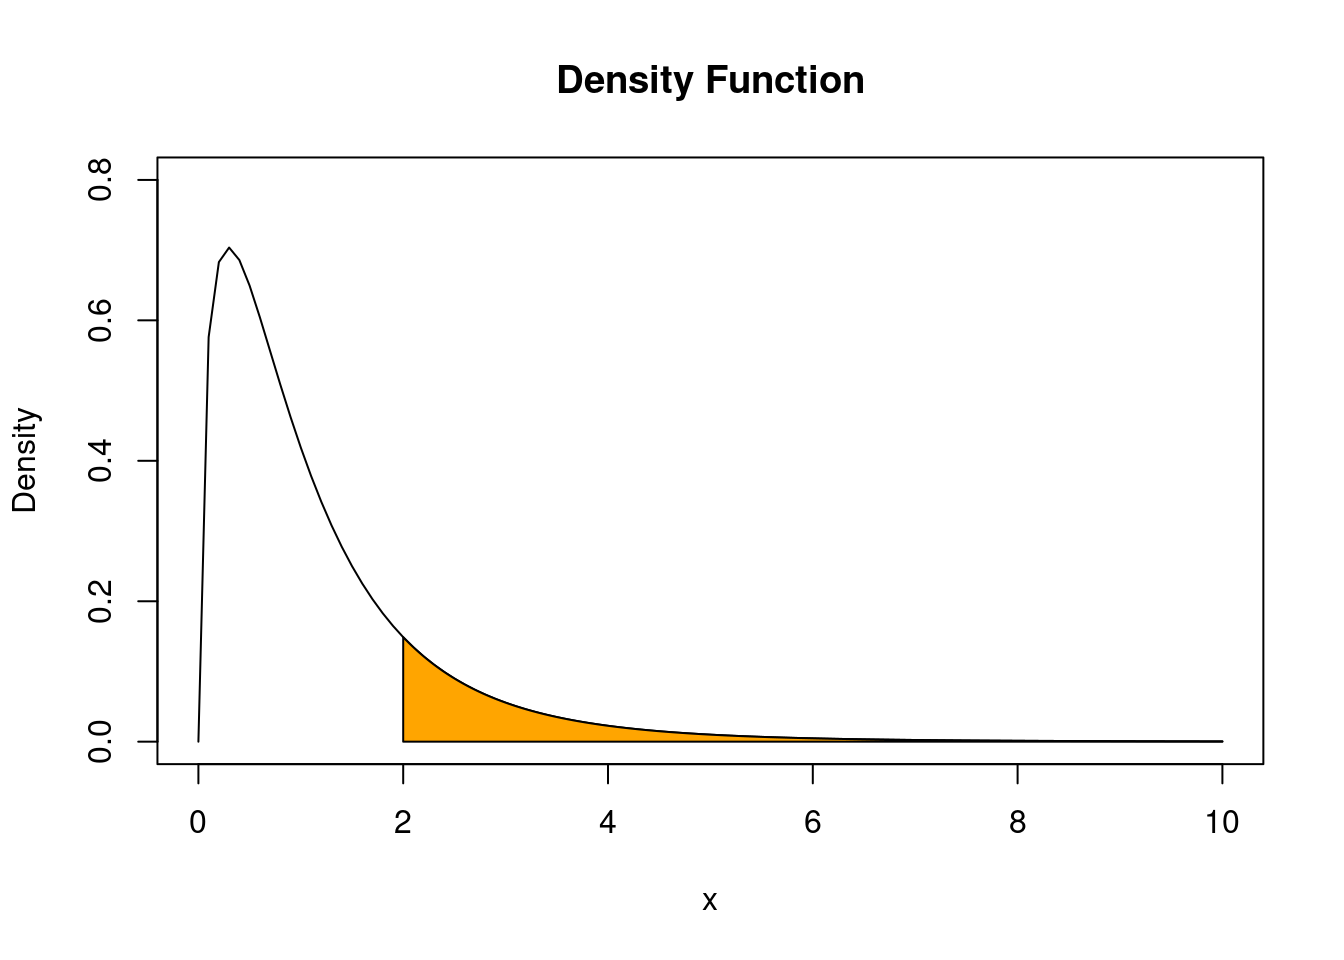
\includegraphics[width=0.8\linewidth]{figure/minimal-unnamed-chunk-51-1} \end{center}

The \(F\) distribution is related to many other distributions. An important special case encountered in econometrics arises if the denominator degrees of freedom are large such that the \(F_{M,n}\) distribution can be approximated by the \(F_{M,\infty}\) distribution which turns out to be simply the distribution of a \(\chi^2_M\) random variable divided by its degrees of freedom \(M\), i.e.~
\[ 
W/M \sim F_{M,\infty} \quad\text{with}\quad W \sim \chi^2_M.
\]

\hypertarget{ch:MLR}{%
\chapter{Multiple Linear Regression}\label{ch:MLR}}

\paragraph*{Preamble.}

In the following we focus on case of random designs \(X\) (i.e.~\(X\) being a random variable),
since, first, this is the more relevant case in econometrics and, second, it includes the case of
fixed designs (i.e.~\(X\) being deterministic) as a special case (``degenerated random variable'\,').
Caution: A random \(X\) requires us to consider conditional means and variances \say{given $X$}.
That is, if we would be able to resample from the model, we do so by fixing (conditioning on)
the in-principle random explanatory variable \(X\).

\hypertarget{assumptions}{%
\section{Assumptions}\label{assumptions}}

The multiple linear regression model is defined by the following assumptions:

\paragraph*{Assumption 1: The Linear Model Assumption (Data Generating Process)}

\begin{eqnarray}\label{LinMod}
  Y_i&=&\sum_{k=1}^K\beta_k X_{ik}+\varepsilon_i, \quad i=1,\dots,n.
\end{eqnarray}
Usually, a constant (intercept) is included, in this case \(X_{i1}=1\) for all \(i\).
In the following we will always assume that \(X_{i1}=1\) for all \(i\), unless otherwise stated.\\
It is convenient to write equation \eqref{LinMod} using matrix notation
\begin{eqnarray*}
  Y_i&=&\underset{(1\times K)}{X_i'}\underset{(K\times 1)}{\beta} +\varepsilon_i, \quad i=1,\dots,n,
\end{eqnarray*}
where \(X_i=(X_{i1},\dots,X_{iK})'\) and \(\beta=(\beta_1,\dots,\beta_K)'\). Stacking all individual rows \(i\) leads to
\begin{eqnarray}\label{LM}
  \underset{(n\times 1)}{Y}&=&\underset{(n\times K)}{X}\underset{(K\times 1)}{\beta} + \underset{(n\times 1)}{\eps},
\end{eqnarray}
where
\begin{equation*}
Y=\left(\begin{matrix}Y_1\\ \vdots\\Y_n\end{matrix}\right),\quad X=\left(\begin{matrix}X_{11}&\dots&X_{1K}\\\vdots&\ddots&\vdots\\ X_{n1}&\dots&X_{nK}\\\end{matrix}\right),\quad\text{and}\quad \eps=\left(\begin{matrix}\varepsilon_1\\ \vdots\\ \varepsilon_n\end{matrix}\right).
\end{equation*}

\bigskip

Moreover, we assume that the observed (\say{obs}) data points
\[((Y_{1,obs},X_{11,obs},\dots,X_{1K,obs}),(Y_{2,obs},X_{21,obs},\dots,X_{2K,obs}),\dots,(Y_{n,obs},X_{n1,obs},\dots,X_{nK,obs}))\]
are a realizations of an \textbf{independent and identically distributed (i.i.d.)} random sample
\[((Y_{1},X_{11},\dots,X_{1K}),(Y_{2},X_{21},\dots,X_{2K}),\dots,(Y_{n},X_{n1},\dots,X_{nK}))\]

That is, the \(i\)th observed \(K+1\) dimensional data point
\((Y_{i,obs},X_{i1,obs},\dots,X_{iK,obs})\in\mathbb{R}^{K+1}\)
is a realization of a \(K+1\) dimensional random variable
\((Y_{i},X_{i1},\dots,X_{iK})\in\mathbb{R}^{K+1}\),
where \((Y_{i},X_{i1},\dots,X_{iK})\) has the identical joint distribution as
\((Y_{j},X_{j1},\dots,X_{jK})\) for all \(i=1,\dots,n\) and all \(j=1,\dots,n\),
and where
\((Y_{i},X_{i1},\dots,X_{iK})\) is independent of
\((Y_{j},X_{j1},\dots,X_{jK})\) for all \(i\neq j=1,\dots,n\).

Note: Due to \eqref{LinMod}, this i.i.d. assumption is equivalent to assuming that the multivariate
random variables \((\varepsilon_i,X_{i1},\dots,X_{iK})\in\mathbb{R}^{K+1}\) are i.i.d. across
\(i=1,\dots,n\).

\textbf{Remark:} Usually, we do not use a different notation for observed realizations
\((Y_{i,obs},X_{i1,obs},\dots,X_{iK,obs})\in\mathbb{R}^{K+1}\)
and for the corresponding random variable
\((Y_{i},X_{i1},\dots,X_{iK})\in\mathbb{R}^{K+1}\)
since often both interpretations (random variable and its realizations) can make sense
in the same statement and then it depends on the considered context whether the random variables
point if view or the realization point of view applies.

\paragraph*{Assumption 2: Exogeneity}

\[E(\varepsilon_i|X_i)=0,\quad i=1,\dots,n\]
This assumption demands that the mean of the random error term \(\eps_i\) is zero irrespective of the realizations of \(X_i\). Note that together with the random sampling assumption (in Assumption 1) this assumption implies even \textbf{strict} exogeneity \(E(\eps_i|X) = 0\) since we have independence across \(i=1,\dots,n\). Under strict exogeneity, the mean of \(\eps_i\) is zero irrespective of the realizations of \(X_1,\dots,X_n\). The exogeneity assumption is also called \say{orthogonality assumption} or \say{mean independence assumption}.

\paragraph*{Assumption 3: Rank Condition (no perfect multicollinearity)}

\[\rank(X)=K\quad\text{a.s.}\]
This assumption demands that the event of one explanatory variable being linearly dependent on the others occurs with a probability equal to zero. (This is the literal translation of the ``almost surely (a.s.)'' concept.) The assumption implies that \(n\geq K\).

This assumption is a bit dicey and its violation belongs to one of the classic problems in applied econometrics (keywords: multicollinearity, dummy variable trap, variance inflation). The violation of this assumption harms any economic interpretation as we cannot disentangle the explanatory variables' individual effects on \(Y\). Therefore, this assumption is also often called an \emph{identification} assumption.

\paragraph*{Assumption 4: Error distribution.}

Depending on the context (i.e., parameter estimation vs.~hypothesis testing and small \(n\) vs.~large \(n\)) there are different more or less restrictive assumptions. Some of the most common ones are the following (see also Chapter \ref{distrerror} for a detailed discussion about homoscedastic and heteroscedastic error terms):

\begin{itemize}
\item\textbf{Conditional Distribution} $\varepsilon_i|X_i \sim f_{\varepsilon|X}$ for all $i=1,\dots,n$ and for any distribution $f_{\varepsilon|X}$ such that $\varepsilon_i|X_i$ has two (or more) finite moments.
\item\textbf{Conditional Normal Distribution} $\varepsilon_i|X_i \sim \mathcal{N}(0,\sigma^2(X_i))$ for all $i=1,\dots,n$.
\item\textbf{i.i.d.} $\varepsilon_i\overset{\operatorname{i.i.d.}}{\sim}f_\varepsilon$  for all $i=1,\dots,n$ and for any distribution $f_\varepsilon$ such that $\varepsilon_i$ has two (or more) finite moments.\\ 
\textbf{Caution:} Assuming that the error terms $\varepsilon_i$ are themselves i.i.d. across $i=1,\dots,n$ implies that they do not depend on $X_i$. 
\item\textbf{i.i.d. Normal.} As above, but with $f=\mathcal{N}(0,1)$, i.e., $\varepsilon_i\overset{\operatorname{i.i.d.}}{\sim}\mathcal{N}(0,\sigma^2)$ for all $i=1,\dots,n$. 
\item \textbf{Spherical errors (\say{Gauss-Markov assumptions}).} The conditional distributions of  $\varepsilon_i|X_i$ may generally depend on $X_i$, but without affecting the second moments such that
\begin{align*}
E(\varepsilon_i^2|X_i)         &=\sigma^2>0\quad\text{for all }i=1,\dots,n\\
E(\varepsilon_i\varepsilon_j|X)&=0\quad\text{for all }i\neq j\quad\text{with}\quad i=1,\dots,n\quad\text{and}\quad j=1,\dots,n.
\end{align*}
Thus, here one assumes that, for a given realization of $X_i$, the error process is uncorrelated (i.e. $\Cov(\eps_i,\eps_j|X)=E(\eps_i\eps_j|X)=0$ for all $i\neq j$) and homoscedastic (i.e. $\V(\eps_i|X)=\sigma^2$ for all $i$).



\paragraph*{Technical Note.} When we write that $\V(\varepsilon_i|X)=\sigma^2$ or $\V(\eps_i|X_i)=\sigma^2_i$, we implicitly assume that these second moments exists and that they are finite. 
\end{itemize}

\hypertarget{homoscedastic-versus-heteroscedastic-error-terms}{%
\subsubsection*{Homoscedastic versus Heteroscedastic Error Terms}\label{homoscedastic-versus-heteroscedastic-error-terms}}
\addcontentsline{toc}{subsubsection}{Homoscedastic versus Heteroscedastic Error Terms}

The i.i.d. assumption is not as restrictive as it may seem on first sight.\\
It allows for dependence \textit{between} \(\varepsilon_i\) and \((X_{i1},\dots,X_{iK})\in\mathbb{R}^K\).
That is, the error term \(\varepsilon_i\) can have a conditional distribution which depends on
\((X_{i1},\dots,X_{iK})\) (see Chapter \ref{condDistr}).

The exogeneity assumption (Assumption 2: Exogeneity) requires that the conditional mean of
\(\varepsilon_i\) is independent of \(X_i\). Besides this, dependencies between
\(\varepsilon_i\) and \(X_{i1},\dots,X_{iK}\) are allowed.
For instance, the variance of \(\varepsilon_i\) can be a function of \(X_{i1},\dots,X_{iK}\).
If this is the case, \(\varepsilon_i\) is said to be \textbf{heteroscedastic}.

\begin{description}
\item[Heteroscedastic error terms:] The conditional variances 
$\V(\varepsilon_i|X_i=x_i)=\sigma^2(x_i)$ are equal to a 
non-constant variance-function $\sigma^2(x_i)>0$ which is a function of the 
realization $x_i\in\mathbb{R}^K$ of $X_i\in\mathbb{R}^K$. 
\end{description}

\textbf{Example:} \(\varepsilon_i|X_i\sim U[-0.5|X_{i2}|, 0.5|X_{i2}|]\),
with \(X_{i2}\sim U[-4,4]\). This error term is mean independent of \(X_i\)
since \(\E(\varepsilon_i|X_i)=0\), but it has a heteroscedastic conditional variance
since \(\V(\varepsilon_i|X_i)=\frac{1}{12}X_i^2\) depends on \(X_i\).

Sometimes, we need to be more restrictive by assuming that also the variances of the error terms
\(\varepsilon_i\) are independent from \(X_i\). (Higher moments may still depend on \(X_i\).)
This assumption leads to \textbf{homoscedastic} error terms.

\begin{description}
\item[Homoscedastic error terms:] The conditional variances 
$\V(\varepsilon_i|X_i=x_i)=\sigma^2$ are equal to some constant $\sigma^2>0$ for every possible 
realization $x_i\in\mathbb{R}^K$ of $X_i\in\mathbb{R}^K$. 
\end{description}

\bigskip

Sometimes, we need to be even more restrictive by assuming that the error terms \(\varepsilon_i\)
are themselves \textbf{i.i.d.} across \(i=1,\dots,n\). This is more restrictive than the assumption that the
multivariate random variables \((\varepsilon_i,X_{i1},\dots,X_{iK})\) are i.i.d. across \(i=1,\dots,n\)
since it implies that the whole distribution (not only the first two moments) of \(\varepsilon_i\)
does not depend on \(X_i\). This assumption also implies \textbf{homoscedastic} error terms since when
the whole distribution of \(\varepsilon_i\) does not depend on \(X_i\in\mathbb{R}^K\) also its variance
doesn't depend on \(X_i\). \textbf{Example:} For doing small sample inference (see Chapter \ref{ch:SSINF}), we need to assume that the error terms \(\varepsilon_i\) are i.i.d. across \(i=1,\dots,n\) plus the normality assumption, i.e., \(\varepsilon_i\stackrel{\textrm{i.i.d.}}{\sim}{\mathcal N} (0, \sigma^2)\) for all \(i=1,\dots,n\) which leads to homoscedastic variances \(\V(\varepsilon_i|X_i)=\sigma^2\) for every possible realization of \(X_i\).

\hypertarget{some-implications-of-the-exogeneity-assumption}{%
\subsection{Some Implications of the Exogeneity Assumption}\label{some-implications-of-the-exogeneity-assumption}}

\begin{itemize}
\item[\textbf{(a)}] If $E(\eps_i|X_i)=0$ for all $i=1,\dots,n$, then the unconditional mean of the error term is zero, i.e.
\begin{eqnarray*}
  E(\eps_i)&=&0,\quad i=1,\dots,n
\end{eqnarray*}
%%%%%%%%%%%%%%%%%%%%%%%%%%%%%%%%%%%%%%%%%%%%%%%%%%%%%%%%%%%
\begin{mdframed}[hidealllines=true,backgroundcolor=blue!20]
Proof: % Hayashi p.9
%%%%%%%%%%%%%%%%%%%%%%%%%%%%%%%%%%%%%%%%%%%%%%%%%%%%%%%%%%%
Using the \emph{Law of Total Expectations} (i.e., $E[E(Z|X)]=E(Z)$) we can rewrite $E(\eps_i)$ as
$$E(\eps_i)=E[E(\eps_i|X_i)],\;\text{for all}\;i=1,\dots,n.$$
But the exogeneity assumption yields
$$E[E(\eps_i|X_i)]=E[0]=0\;\text{for all}\;i=1,\dots,n,$$
which completes the proof. $\square$
%%%%%%%%%%%%%%%%%%%%%%%%%%%%%%%%%%%%%%%%%%%%%%%%%%%%%%%%%%%
\end{mdframed}
\item[\textbf{(b)}] Exogeneity is sometimes also called orthogonality--the reason is the following.  Generally, two random variables $X$ and $Y$ are said to be \textbf{orthogonal} if their cross moment is zero, i.e. if $E(XY)=0$.\\[2ex] \noindent Under exogeneity, i.e. if $E(\eps_i|X_{i})=0$, the regressors and the error term are orthogonal to each other, i.e,
\begin{eqnarray*}
E(X_{ik}\eps_i)&=&0\quad\text{for all}\quad i=1,\dots,n\quad\text{and}\quad k=1,\dots,K.
\end{eqnarray*}
%%%%%%%%%%%%%%%%%%%%%%%%%%%%%%%%%%%%%%%%%%%%%%%%%%%%%%%%%%%
\begin{mdframed}[hidealllines=true,backgroundcolor=blue!20]
Proof: % Hayashi p.9
%%%%%%%%%%%%%%%%%%%%%%%%%%%%%%%%%%%%%%%%%%%%%%%%%%%%%%%%%%%
\begin{eqnarray*}
  E(X_{ik}\eps_i)&=&E(E(X_{ik}\eps_i|X_{ik}))\quad{\small\text{(By the Law of Total Expectations)}}\\
  &=&E(X_{ik}E(\eps_i|X_{ik}))\quad{\small\text{(By the linearity of cond.~expectations)}}
\end{eqnarray*}
Now, to show that $E(X_{ik}\eps_i)=0$, we need to show that $E(\eps_i|X_{ik})=0$, which is done in the following:\\
Since $X_{ik}$ is an element of $X_i$, a slightly more sophisticated use of the \emph{Law of Total Expectations} (i.e., $E(Y|X)=E(E(Y|X,Z)|X)$) implies that
$$E(\eps_i|X_{ik})=E(E(\eps_i|X_i)|X_{ik}).$$
So, the exogeneity assumption, $E(\eps_i|X_i)=0$ yields
$$E(\eps_i|X_{ik})=E(\underbrace{E(\eps_i|X_i)}_{=0}|X_{ik})=E(0|X_{ik})=0.$$
I.e., we have that $E(\eps_i|X_{ik})=0$ which allows us to conclude that
$$E(X_{ik}\eps_i)=E(X_{ik}E(\eps_i|X_{ik}))=E(X_{ik}0)=0.\quad\square$$
\end{mdframed}
%%%%%%%%%%%%%%%%%%%%%%%%%%%%%%%%%%%%%%%%%%%%%%%%%%%%%%%%%%%
\item[\textbf{(c)}] Because the mean of the error term is zero ($E(\eps_i)=0$ for all $i$; see point (a)), it follows that the orthogonality property ($E(X_{ik}\eps_i)=0$) is equivalent to a zero-correlation property.  I.e., if $E(\eps_i|X_{i})=0$, then 
\begin{eqnarray*}
  \Cov(\eps_i,X_{ik})&=&0\quad\text{for all}\quad i=1,\dots,n\quad\text{and}\quad k=1,\dots,K.
\end{eqnarray*}
%%%%%%%%%%%%%%%%%%%%%%%%%%%%%%%%%%%%%%%%%%%%%%%%%%%%%%%%%%%
\begin{mdframed}[hidealllines=true,backgroundcolor=blue!20]
Proof: % Hayashi p.9
%%%%%%%%%%%%%%%%%%%%%%%%%%%%%%%%%%%%%%%%%%%%%%%%%%%%%%%%%%%
\begin{eqnarray*}
  \Cov(\eps_i,X_{ik})&=&E(X_{ik}\eps_i)-E(X_{ik})\,E(\eps_i)\quad{\small\text{(Def. of Cov)}}\\
  &=&E(X_{ik}\eps_i)\quad{\small\text{(By point (a): $E(\eps_i)=0$)}}\\
  &=&0\quad{\small\text{(By orthogonality result in point (b))}}\quad\square
\end{eqnarray*}
\end{mdframed}
\end{itemize}

\hypertarget{deriving-the-expression-of-the-ols-estimator}{%
\section{Deriving the Expression of the OLS Estimator}\label{deriving-the-expression-of-the-ols-estimator}}

Similar to Section \ref{sec:SLROLS}, we can derive the expression for the OLS estimator \(\hat\beta=(\hat\beta_1,\dots,\hat\beta_K)'\in\mathbb{R}^K\) as the vector-valued minimizing argument of the sum of squared residuals, \(S_n(b)\) with \(b\in\mathbb{R}^K\), for a given sample \(((Y_1,X_1),\dots,(Y_n,X_n))\). In matrix terms this is
\begin{align*}
S_n(b)&=(Y-X b)^{\prime}(Y-X b)=Y^{\prime}Y-2 Y^{\prime} X b+b^{\prime} X^{\prime} X b.
\end{align*}
To find the minimizing argument \[\hat\beta=\arg\min_{b\in\mathbb{R}^K}S_n(b)\] we compute all partial derivatives
\[
\begin{aligned}
\underset{(K\times 1)}{\frac{\partial S(b)}{\partial b}} &=-2\left(X^{\prime}Y -X^{\prime} Xb\right).
\end{aligned}
\]
and set them equal to zero which leads to \(K\) linear equations (the \say{normal equations}) in \(K\) unknowns. This system of equations defines the OLS estimates, \(\hat{\beta}\), for a given data-set:
\[
\begin{aligned}
-2\left(X^{\prime}Y -X^{\prime} X\hat{\beta}\right)=\underset{(K\times 1)}{0}.
\end{aligned}
\]
From our rank assumption (Assumption 3) it follows that \(X^{\prime}X\) is an invertible matrix which allows us to solve the equation system by
\[
\begin{aligned}
\underset{(K\times 1)}{\hat{\beta}} &=\left(X^{\prime} X\right)^{-1} X^{\prime} Y
\end{aligned}
\]

The following codes computes the estimate \(\hat{\beta}\) for a given realization \((Y,X)\) of the random sample \((Y,X)\).

\begin{Shaded}
\begin{Highlighting}[]
\CommentTok{\# Some given data}
\NormalTok{X\_1 }\OtherTok{\textless{}{-}} \FunctionTok{c}\NormalTok{(}\FloatTok{1.9}\NormalTok{,}\FloatTok{0.8}\NormalTok{,}\FloatTok{1.1}\NormalTok{,}\FloatTok{0.1}\NormalTok{,}\SpecialCharTok{{-}}\FloatTok{0.1}\NormalTok{,}\FloatTok{4.4}\NormalTok{,}\FloatTok{4.6}\NormalTok{,}\FloatTok{1.6}\NormalTok{,}\FloatTok{5.5}\NormalTok{,}\FloatTok{3.4}\NormalTok{)}
\NormalTok{X\_2 }\OtherTok{\textless{}{-}} \FunctionTok{c}\NormalTok{(}\DecValTok{66}\NormalTok{, }\DecValTok{62}\NormalTok{, }\DecValTok{64}\NormalTok{, }\DecValTok{61}\NormalTok{, }\DecValTok{63}\NormalTok{, }\DecValTok{70}\NormalTok{, }\DecValTok{68}\NormalTok{, }\DecValTok{62}\NormalTok{, }\DecValTok{68}\NormalTok{, }\DecValTok{66}\NormalTok{)}
\NormalTok{Y   }\OtherTok{\textless{}{-}} \FunctionTok{c}\NormalTok{(}\FloatTok{0.7}\NormalTok{,}\SpecialCharTok{{-}}\FloatTok{1.0}\NormalTok{,}\SpecialCharTok{{-}}\FloatTok{0.2}\NormalTok{,}\SpecialCharTok{{-}}\FloatTok{1.2}\NormalTok{,}\SpecialCharTok{{-}}\FloatTok{0.1}\NormalTok{,}\FloatTok{3.4}\NormalTok{,}\FloatTok{0.0}\NormalTok{,}\FloatTok{0.8}\NormalTok{,}\FloatTok{3.7}\NormalTok{,}\FloatTok{2.0}\NormalTok{)}
\NormalTok{dataset }\OtherTok{\textless{}{-}}  \FunctionTok{cbind.data.frame}\NormalTok{(X\_1,X\_2,Y)}
\DocumentationTok{\#\# Compute the OLS estimation}
\NormalTok{my.lm }\OtherTok{\textless{}{-}} \FunctionTok{lm}\NormalTok{(Y }\SpecialCharTok{\textasciitilde{}}\NormalTok{ X\_1 }\SpecialCharTok{+}\NormalTok{ X\_2, }\AttributeTok{data =}\NormalTok{ dataset)}
\DocumentationTok{\#\# Plot sample regression surface}
\FunctionTok{library}\NormalTok{(}\StringTok{"scatterplot3d"}\NormalTok{) }\CommentTok{\# library for 3d plots}
\NormalTok{plot3d }\OtherTok{\textless{}{-}} \FunctionTok{scatterplot3d}\NormalTok{(}\AttributeTok{x =}\NormalTok{ X\_1, }\AttributeTok{y =}\NormalTok{ X\_2, }\AttributeTok{z =}\NormalTok{ Y,}
          \AttributeTok{angle=}\DecValTok{33}\NormalTok{, }\AttributeTok{scale.y=}\FloatTok{0.8}\NormalTok{, }\AttributeTok{pch=}\DecValTok{16}\NormalTok{,}
          \AttributeTok{color =}\StringTok{"red"}\NormalTok{, }\AttributeTok{main =}\StringTok{"OLS Regression Surface"}\NormalTok{)}
\NormalTok{plot3d}\SpecialCharTok{$}\FunctionTok{plane3d}\NormalTok{(my.lm, }\AttributeTok{lty.box =} \StringTok{"solid"}\NormalTok{, }\AttributeTok{col=}\FunctionTok{gray}\NormalTok{(.}\DecValTok{5}\NormalTok{), }
          \AttributeTok{draw\_polygon=}\ConstantTok{TRUE}\NormalTok{)}
\end{Highlighting}
\end{Shaded}

\begin{center}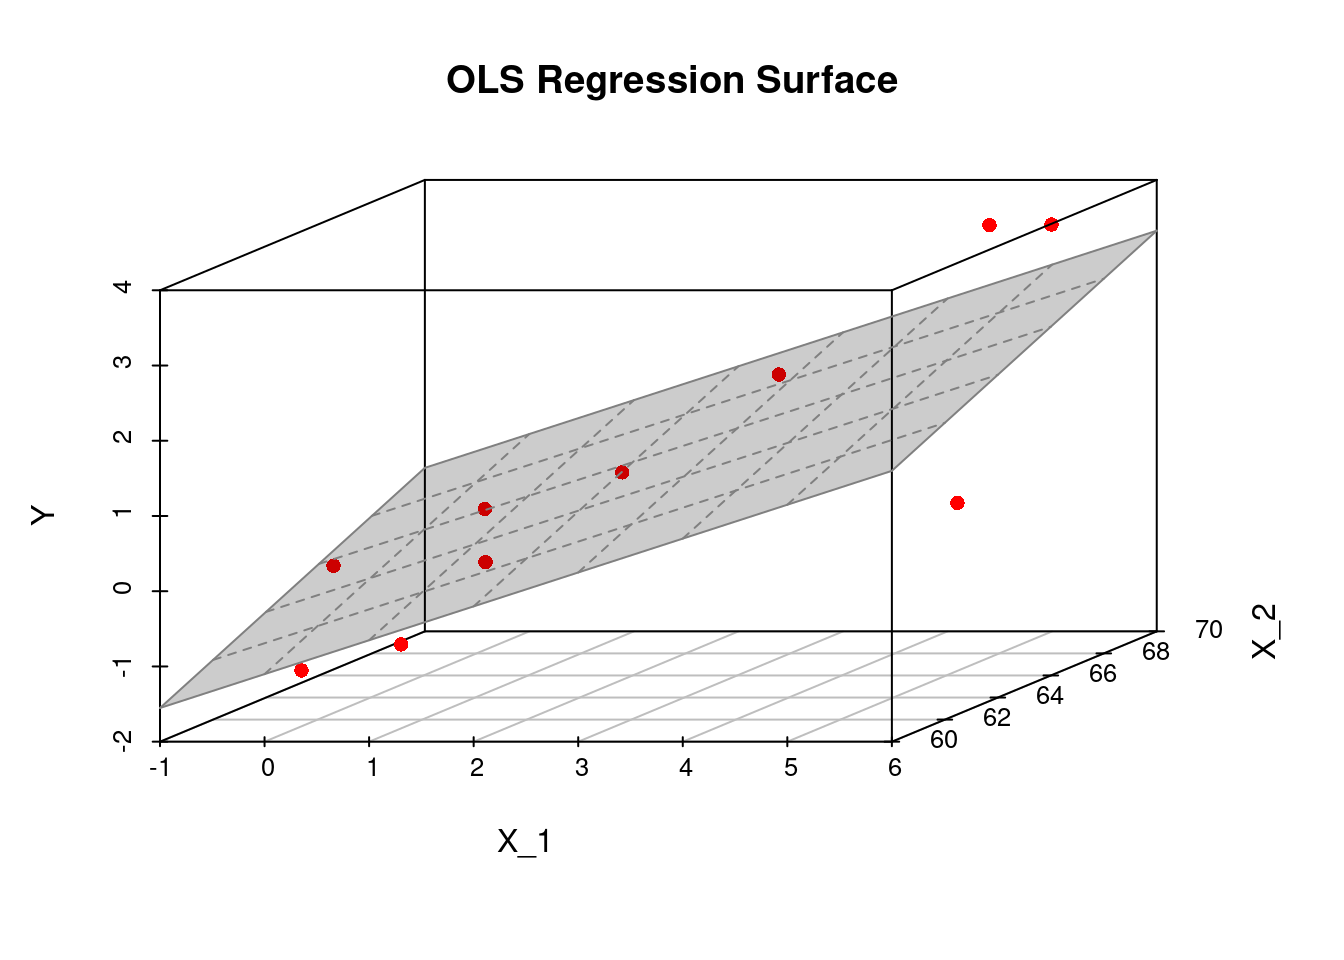
\includegraphics[width=0.8\linewidth]{figure/minimal-unnamed-chunk-52-1} \end{center}

\hypertarget{some-quantities-of-interest}{%
\section{Some Quantities of Interest}\label{some-quantities-of-interest}}

\paragraph*{Predicted values and residuals.} 
\begin{itemize}
\item The (OLS) \textbf{predicted values}: $\hat{Y}_i=X_i'\hat\beta$\\
In matrix notation: $\hat Y=X\underbrace{(X'X)^{-1}X'Y}_{\hat\beta}=P_X Y$
\item The (OLS) \textbf{residual}: $\hat\eps_i=Y_i-\hat{Y}_i$\\
In matrix notation: $\hat\eps=Y-\hat{Y}=\left(I_n-X(X'X)^{-1}X'\right)Y=M_X Y$
%\item Population regression (hyper-)surface: $E[Y|X]=X\beta$ 
%\item Sample regression (hyper-)surface: $\widehat{E[Y|X]}=\hat Y=X\hat\beta$ 
\end{itemize}

\paragraph*{Projection matrices.}

The matrix \(P_X=X(X'X)^{-1}X'\) is the \((n\times n)\) \textbf{projection matrix} that projects any vector (from \(\mathbb{R}^n\)) into the column space spanned by the column vectors of \(X\) and \(M_X=I_n-X(X'X)^{-1}X'=I_n-P_X\) is the associated \((n\times n)\) \textbf{orthogonal projection matrix} that projects any vector (from \(\mathbb{R}^n\)) into the vector space that is orthogonal to that spanned by \(X\).

The projection matrices \(P_X\) and \(M_X\) have some nice properties:

\begin{itemize}
\item[(a)] $P_X$ and $M_X$ are symmetric, i.e. $P_X=P_X'$ and $M_X=M_X'$.
\item[(b)] $P_X$ and $M_X$ are idempotent, i.e. $P_XP_X=P_X$ and $M_X M_X=M_X$.
\item[(c)] Moreover $X'P_X=X'$, $P_XX=X$, $X'M_X=0$, $M_XX=0$, and $P_XM_X=0$.
\end{itemize}

All of these properties follow directly from the definitions of \(P_X\) and \(M_X\) (check it out). Using these properties one can show that the residual vector \(\hat\eps=(\hat\eps_1,\dots,\hat\eps_n)'\) is orthogonal to each of the column vectors in \(X\), i.e
\begin{eqnarray}
X'\hat\eps&=&X'M_XY\quad\text{\small(By Def.~of $M_X$)}\notag\\
\Leftrightarrow X'\hat\eps&=&\underset{(K\times n)}{0}\underset{(n\times 1)}{Y}\quad\text{\small(since $X'M_X=0$)}\notag\\
\Leftrightarrow X'\hat\eps&=&\underset{(K\times 1)}{0}\label{eq:orthXe}
\end{eqnarray}
Note that, in the case with intercept \eqref{eq:orthXe} implies that \(\sum_{i=1}^n\hat\eps_i=0\). Moreover, equation \eqref{eq:orthXe} implies also that the residual vector \(\hat{\eps}\) is orthogonal to the predicted values vector, since
\begin{align*}
X'\hat\eps&=0\\
\Rightarrow\;\hat\beta'X'\hat\eps&=\hat\beta'0\\
\Leftrightarrow\;\hat Y'\hat\eps&=0.
\end{align*}

Another insight from equation \eqref{eq:orthXe} is that the vector \(\hat\eps\) has to satisfy \(K\) linear restrictions (\(X'\hat\eps=0\)) which means it looses \(K\) degrees of freedom. Consequently, the vector of residuals \(\hat\eps\) has only \(n-K\) so-called \emph{degrees of freedom}. This loss of \(K\) degrees of freedom also appears in the definition of the \emph{unbiased} variance estimator
\begin{align}
  s_{UB}^2&=\frac{1}{n-K}\sum_{i=1}^n\hat\eps_i^2\label{EqVarEstim}.
\end{align}

\paragraph*{Variance decomposition.}

A further useful result that can be shown using the properties of \(P_X\) and \(M_X\) is that \(Y'Y=\hat{Y}'\hat{Y}+\hat\eps'\hat\eps\), i.e.
\begin{eqnarray}
Y'Y&=&(\hat Y+\hat\eps)'(\hat Y+\hat\eps)\notag\\
  &=&(P_XY+M_XY)'(P_XY+M_XY)\notag\\
  &=&(Y'P_X'+Y'M_X')(P_XY+M_XY)\notag\\
  &=&Y'P_X'P_XY+Y'M_X'M_XY+0\notag\\
  &=&\hat{Y}'\hat{Y}+\hat\eps'\hat\eps\label{PropVarDecomp}
\end{eqnarray}
Decomposition \eqref{PropVarDecomp} is the basis for the well-known variance decomposition result for OLS regressions. For the OLS regression of the linear model \eqref{LinMod} with intercept, the total sample variance of the dependent variable \(Y_1,\dots,Y_n\) can be decomposed as following:
\begin{eqnarray}
\underset{\text{total sample variance}}{\frac{1}{n}\sum_{i=1}^n\left(Y_i-\bar{Y}\right)^2}&=&\underset{\text{explained sample variance}}{\frac{1}{n}\sum_{i=1}^n\left(\hat{Y}_i-\bar{\hat{Y}}\right)^2}+\underset{\text{unexplained sample variance}}{\frac{1}{n}\sum_{i=1}^n\hat\eps_i^2,}\label{VarDecomp}
\end{eqnarray}
where \(\bar{Y}=\frac{1}{n}\sum_{i=1}^nY_i\) and likewise for \(\bar{\hat{Y}}\).

\begin{mdframed}[hidealllines=true,backgroundcolor=blue!20]
Proof of \eqref{VarDecomp}:
\begin{itemize}
\item As a consequence of \eqref{eq:orthXe} we have for regressions with intercept that $\sum_{i=1}^n\hat\eps_i=0$. Hence, from $Y_i=\hat{Y}_i+\hat\eps_i$ it follows that
\begin{eqnarray}
  \frac{1}{n}\sum_{i=1}^n Y_i&=&\frac{1}{n}\sum_{i=1}^n \hat{Y}_i+\frac{1}{n}\sum_{i=1}^n \hat\eps_i\notag\\
  \bar{Y}&=&\bar{\hat{Y}}+0\label{eq:aux}
\end{eqnarray}
\item From \eqref{PropVarDecomp} we know that $Y'Y=\hat{Y}'\hat{Y}+\hat\eps'\hat\eps$, i.e.
\begin{eqnarray*}
   Y'Y&=&\hat{Y}'\hat{Y}+\hat\eps'\hat\eps\\
   Y'Y-n\bar{Y}^2&=&\hat{Y}'\hat{Y}-n\bar{Y}^2+\hat\eps'\hat\eps\\
   Y'Y-n\bar{Y}^2&=&\hat{Y}'\hat{Y}-n\bar{\hat{Y}}^2+\hat\eps'\hat\eps\quad\text{(by \eqref{eq:aux} $\bar{Y}=\bar{\hat{Y}}$)}\\
   \sum_{i=1}^nY_i^2-n\bar{Y}^2&=&\sum_{i=1}^n\hat{Y}_i^2-n\bar{\hat{Y}}^2+\sum_{i=1}^n\hat\eps_i^2\\
   \sum_{i=1}^n(Y_i-\bar{Y})^2&=&\sum_{i=1}^n(\hat{Y}_i-\bar{\hat{Y}})^2+\sum_{i=1}^n\hat\eps_i^2\quad\square\\
\end{eqnarray*}
\end{itemize}
\end{mdframed}

\paragraph*{Coefficient of determination $R^2$.}

The larger the proportion of the explained variance, the better is the fit of the model. This motivates the definition of the so-called \(R^2\) coefficient of determination:
\begin{eqnarray*}
R^2=\frac{\sum_{i=1}^n\left(\hat{Y}_i-\bar{\hat{Y}}\right)^2}{\sum_{i=1}^n\left(Y_i-\bar{Y}\right)^2}\;=\;1-\frac{\sum_{i=1}^n\hat{\eps}_i^2}{\sum_{i=1}^n\left(Y_i-\bar{Y}\right)^2}
\end{eqnarray*}
Obviously, we have that \(0\leq R^2\leq 1\). The closer \(R^2\) lies to \(1\), the better is the fit of the model to the observed data. However, a high/low \(R^2\) does not mean a validation/falsification of the estimated model. Any relation (i.e., model assumption) needs a plausible explanation from relevant economic theory. The most often criticized disadvantage of the \(R^2\) is that additional regressors (relevant or not) will always increase the \(R^2\). Here is an example of the problem.

\begin{Shaded}
\begin{Highlighting}[]
\FunctionTok{set.seed}\NormalTok{(}\DecValTok{123}\NormalTok{)}
\NormalTok{n     }\OtherTok{\textless{}{-}} \DecValTok{100}               \CommentTok{\# Sample size}
\NormalTok{X     }\OtherTok{\textless{}{-}} \FunctionTok{runif}\NormalTok{(n, }\DecValTok{0}\NormalTok{, }\DecValTok{10}\NormalTok{)   }\CommentTok{\# Relevant X variable}
\NormalTok{X\_ir  }\OtherTok{\textless{}{-}} \FunctionTok{runif}\NormalTok{(n, }\DecValTok{5}\NormalTok{, }\DecValTok{20}\NormalTok{)   }\CommentTok{\# Irrelevant X variable}
\NormalTok{error }\OtherTok{\textless{}{-}} \FunctionTok{rt}\NormalTok{(n, }\AttributeTok{df =} \DecValTok{10}\NormalTok{)}\SpecialCharTok{*}\DecValTok{10}  \CommentTok{\# True error}
\NormalTok{Y     }\OtherTok{\textless{}{-}} \DecValTok{1} \SpecialCharTok{+} \DecValTok{5} \SpecialCharTok{*}\NormalTok{ X }\SpecialCharTok{+}\NormalTok{ error    }\CommentTok{\# Y variable}
\NormalTok{lm1   }\OtherTok{\textless{}{-}} \FunctionTok{summary}\NormalTok{(}\FunctionTok{lm}\NormalTok{(Y}\SpecialCharTok{\textasciitilde{}}\NormalTok{X))     }\CommentTok{\# Correct OLS regression }
\NormalTok{lm2   }\OtherTok{\textless{}{-}} \FunctionTok{summary}\NormalTok{(}\FunctionTok{lm}\NormalTok{(Y}\SpecialCharTok{\textasciitilde{}}\NormalTok{X}\SpecialCharTok{+}\NormalTok{X\_ir))}\CommentTok{\# OLS regression with X\_ir }
\NormalTok{lm1}\SpecialCharTok{$}\NormalTok{r.squared }\SpecialCharTok{\textless{}}\NormalTok{ lm2}\SpecialCharTok{$}\NormalTok{r.squared}
\CommentTok{\#\textgreater{} [1] TRUE}
\end{Highlighting}
\end{Shaded}

So, \(R^2\) increases here even though \texttt{X\_ir} is a completely irrelevant explanatory variable. Because of this, the \(R^2\) cannot be used as a criterion for model selection. Possible solutions are given by penalized criterions such as the so-called \emph{adjusted $R^2$} defined as
\begin{eqnarray*}
  \overline{R}^2&=&1-\frac{\frac{1}{n-K}\sum_{i=1}^n\hat{\eps}^2_i}{\frac{1}{n-1}\sum_{i=1}^n\left(Y_i-\bar{Y}\right)^2}\leq R^2%\\
  %=\dots=
  %&=&1-\frac{n-1}{n-K}\left(1-R^2\right)\quad{\small\text{(since $1-R^2=(\sum_i\hat\eps_i^2)/(\sum_i(Y_i-\bar{Y}))$)}}\\
  %&=&1-\frac{n-1}{n-K}+\frac{n-1}{n-K}R^2\quad+\frac{K-1}{n-K}R^2-\frac{K-1}{n-K}R^2\\
  %&=&1-\frac{n-1}{n-K}+R^2\quad+\frac{K-1}{n-K}R^2\\
  %&=&-\frac{K-1}{n-K}+R^2\quad+\frac{K-1}{n-K}R^2\\
  %&=&R^2-\underbrace{\frac{K-1}{n-K}\left(1-R^2\right)}_{\geq 0\;\text{and}\;\leq(K-1)/(n-K)}\;\leq\;R^2
\end{eqnarray*}
The adjustment is in terms of the degrees of freedom \(n-K\).

\hypertarget{method-of-moments-estimator}{%
\section{Method of Moments Estimator}\label{method-of-moments-estimator}}

The methods of moments estimator exploits the exogeneity assumption that \(E(\eps_i|X_i)=0\) for all \(i=1,\dots,n\) (Assumption 2). Remember that \(E(\eps_i|X_i)=0\) implies that \(E(X_{ik}\eps_i)=0\) for all \(i=1,\dots,n\) and all \(k=1,\dots,K\). The fundamental idea behind \say{method of moments estimation} is to use the sample analogues of these population moment restrictions \(E(X_{ik}\eps_i)=0\), \(k=1,\dots,K\), for deriving the estimator:
\[
\begin{array}{c||c}
\text{$K$ population moment restrictions\quad}&\text{$K$ sample moment restrictions}\\[2ex]
\left.\begin{array}{c}
E(\eps_i)=0\\
E(X_{i2}\eps_i)=0\\
\vdots\\
E(X_{iK}\eps_i)=0
\end{array}
\right\}\Leftrightarrow E(X_i\eps_i)=\underset{(K\times 1)}{0} &
\left.\begin{array}{c}
\displaystyle
\frac{1}{n}\sum_{i=1}^n\hat\eps_i=0\\
\displaystyle
\frac{1}{n}\sum_{i=1}^nX_{i2}\hat\eps_i=0\\
\vdots\\
\displaystyle
\frac{1}{n}\sum_{i=1}^nX_{iK}\hat\eps_i=0\\
\end{array}
\right\}\Leftrightarrow \displaystyle\frac{1}{n}\sum_{i=1}^nX_i\hat\eps_i=\underset{(K\times 1)}{0}
\end{array}
\]

Under our set of assumptions (Ass 1-4), the sample means \(n^{-1}\sum_{i=1}^nX_i\hat\eps_i\) are consistent estimators of the population means \(E(X_i\eps_i)\). The idea is now to find \(\hat\beta_0,\dots,\hat\beta_K\) values which lead to residuals \(\hat\eps_i=Y_i-\sum_{k=1}^K\hat\beta_kX_{ik}\) that fulfill the above sample moment restrictions. This should in principle be possible since we have a linear system of \(K\) equations \(\frac{1}{n}\sum_{i=1}^nX_i\hat\eps=0\) and \(K\) unknowns \(\hat\beta=(\hat\beta_0,\dots,\hat\beta_K)'\). Solving the equation system yields,

\begin{align*}
\frac{1}{n}\sum_{i=1}^n X_i\hat\eps_i&=\underset{(K\times 1)}{0}\\
\frac{1}{n}\sum_{i=1}^n X_i\left(Y_i-X_i'\hat\beta\right)&=\underset{(K\times 1)}{0}\\
\frac{1}{n}\sum_{i=1}^n X_i Y_i-\frac{1}{n}\sum_{i=1}^n X_iX_i'\hat\beta &=\underset{(K\times 1)}{0}\\
\frac{1}{n}\sum_{i=1}^n X_iX_i'\hat\beta &=\frac{1}{n}\sum_{i=1}^n X_i Y_i\\
\hat\beta &= \left(\frac{1}{n}\sum_{i=1}^n X_iX_i'\right)^{-1}\frac{1}{n}\sum_{i=1}^n X_i Y_i\\
\hat\beta &= \left(X'X\right)^{-1} X' Y\\
\end{align*}
which equals the OLS estimator of \(\beta\); although, we used now a different approach to derive the estimator.

Once again we see the importance of the exogeneity assumption \(E(\eps_i|X_i)\) which we used here as the starting point for the derivation of the methods of moments estimator. However, unlike with deriving the OLS estimator as the estimator that minimizes the sum of squared residuals, here we derived the estimator
\emph{from the exogeineity assumptions}. The method of moments is a very general method, which usually has good
properties. We will return to the method of moments several times throughout the semester.

\hypertarget{unbiasedness-of-hatbetax-and-hatbeta}{%
\section{\texorpdfstring{Unbiasedness of \(\hat\beta|X\) and \(\hat\beta\)}{Unbiasedness of \textbackslash hat\textbackslash beta\textbar X and \textbackslash hat\textbackslash beta}}\label{unbiasedness-of-hatbetax-and-hatbeta}}

Once again, but now using matrix algebra, we can show that the OLS (or likewise the Methods-of-Moments estimator) \(\hat\beta = \left(X'X\right)^{-1}X'Y\) is unbiased:
\begin{align*}
E[\hat{\beta}|X]
&=E\left[\left(X^{\prime} X\right)^{-1} X^{\prime} Y|X\right]\\
&=E\left[\left(X^{\prime} X\right)^{-1} X^{\prime}(X \beta+\eps)|X\right] \\
&=E\left[\left(X^{\prime} X\right)^{-1} X^{\prime} X \beta+\left(X^{\prime} X\right)^{-1} X^{\prime} \eps|X\right] \\
&=\beta+E\left[\left(X^{\prime} X\right)^{-1} X^{\prime} \eps|X\right] \\
&=\beta+\left(X^{\prime} X\right)^{-1} X^{\prime}\underbrace{E[\eps|X]}_{=0}=\beta\\
\Leftrightarrow\;\operatorname{Bias}[\hat{\beta}|X]&=0\\
\Leftrightarrow\;\underbrace{E\big(\operatorname{Bias}[\hat{\beta}|X]\big)}_{=\operatorname{Bias}[\hat{\beta}]}&=E(0)\\
\Leftrightarrow\;E\big(\operatorname{Bias}[\hat{\beta}]\big)&=0\\
\end{align*}

\paragraph*{Note.}

This result only requires the strict exogeneity assumption \(E(\eps|X)=0\) which follows from our Assumption 2 (i.e.~\(E(\eps_i|X_i)=0\) for all \(i\)) together with Assumption 1 (i.e.~\((Y_i,X_i)\) is i.i.d. across \(i=1,\dots,n\)). In particular, we did not need to assume homoscedasticity (and it also holds for auto-correlated error terms).

\hypertarget{ch:VarEstBeta}{%
\section{\texorpdfstring{Variance of \(\hat\beta|X\)}{Variance of \textbackslash hat\textbackslash beta\textbar X}}\label{ch:VarEstBeta}}

The conditional variance of \(\hat\beta\) given \(X\) is given by
\begin{align*}
\V(\hat{\beta}|X)=& E\left[(\hat{\beta}-\beta)(\hat{\beta}-\beta)^{\prime}|X\right] \\
=& E\left[\left(\left(X^{\prime} X\right)^{-1} X^{\prime} \eps\right)\left(\left(X^{\prime} X\right)^{-1} X^{\prime} \eps\right)^{\prime}|X\right] \\
=& E\left[\left(X^{\prime} X\right)^{-1} X^{\prime} \eps\eps^{\prime} X\left(X^{\prime} X\right)^{-1}|X\right] \\
=& \left(X^{\prime} X\right)^{-1} X^{\prime} E\left[\eps\eps^{\prime}|X\right] X\left(X^{\prime} X\right)^{-1}\\
=& \underbrace{\left(X^{\prime} X\right)^{-1} X^{\prime} \overbrace{\V(\eps|X)}^{(n\times n)} X\left(X^{\prime} X\right)^{-1}}_{(K\times K)\text{-dimesnional}},\\
\end{align*}
In the above derivations we used, first, that
\begin{align*}
\hat\beta-\beta
&=\left(X^{\prime} X\right)^{-1} X^{\prime} Y-\beta\\
&=\left(X^{\prime} X\right)^{-1} X^{\prime}(X\beta+\eps)-\beta\\
&=\beta+\left(X^{\prime} X\right)^{-1} X^{\prime}\eps)-\beta\\
&=\left(X^{\prime} X\right)^{-1} X^{\prime}\eps
\end{align*}
and, second, that \(E\left[\eps\eps^{\prime}|X\right]=\V(\eps|X)\) since \(E(\eps|X)=0\) under our assumptions. The above expression is the general version of \(\V(\hat{\beta}|X)\) which can be further simplified using specific assumptions on the distribution of the error term \(\eps\):

\begin{itemize}
\item In case of spherical errors (\say{Gauss-Markov assumptions}), i.e. no heteroscedasticity and non auto-correlations, we have that $\V(\eps|X)=\sigma^2 I_n$ such that
$$
\V(\hat{\beta}|X)=\underset{(K\times K)}{\sigma^{2} \left(X^{\prime} X\right)^{-1}}
$$
\item In case of conditional heteroscedasticitiy, we have that $$\V(\eps|X)=\left(\begin{matrix}\sigma_1^2&0&\dots&0\\0&\sigma_2^2&\dots&0\\\vdots&\vdots&\ddots&\vdots\\0&0&\dots&\sigma_n^2\end{matrix}\right)=\operatorname{diag}(\sigma_1^2,\dots,\sigma_n^2),$$
where the variances $\sigma_i^2$ may be functions of $X_i$, i.e. $\sigma^2_i\equiv\sigma_i^2(X_i)$. 
Under conditional heteroscedasticitiy we have the following \say{sandwich} form 
$$
\V(\hat{\beta}|X)=\left(X^{\prime} X\right)^{-1} X^{\prime} \operatorname{diag}(\sigma_1^2,\dots,\sigma_n^2) X\left(X^{\prime} X\right)^{-1}.
$$
\end{itemize}

\paragraph*{Practical estimation of the standard errors.}

The diagonal elements in the \((K\times K)\) matrix \(\V(\hat{\beta}|X)\) are the variance expressions for the single estimators \(\hat\beta_k\) with \(k=1,\dots,K\),
\begin{align*}
\V(\hat{\beta}_k|X)=&\left[\left(X^{\prime} X\right)^{-1} X^{\prime} \V(\eps|X) X\left(X^{\prime} X\right)^{-1}\right]_{kk}\quad\small{\text{(generally)}}\\
=&\sigma^2\left[\left(X^{\prime} X\right)^{-1}\right]_{kk},\hspace*{4cm}\small{\text{(spherical errors)}}
\end{align*}
where \([A]_{kl}\) denotes the \(kl\)th element of \(A\) that is in the \(k\)th row and \(l\)th column of \(A\). Taking square roots leads to the \textbf{standard errors} of the estimators \(\hat\beta_k|X\)
\begin{align*}
\operatorname{SE}(\hat{\beta}_k|X)=&\left(\left[\left(X^{\prime} X\right)^{-1} X^{\prime} \V(\eps|X) X\left(X^{\prime} X\right)^{-1}\right]_{kk}\right)^{1/2}\quad\small{\text{(generally)}}\\
=&\left(\sigma^2\left[\left(X^{\prime} X\right)^{-1}\right]_{kk}\right)^{1/2},\hspace*{4cm}\small{\text{(spherical errors)}}
\end{align*}
Of course, the above expressions for \(\V(\hat{\beta}_k|X)\) and \(\operatorname{SE}(\hat{\beta}_k|X)\) are generally useless in practice since we typically do not know the \((n\times n)\) variance matrix \(\V(\eps|X)\) or \(\sigma^2\), but need to estimate them from the data. So, we typically need to work with
\begin{align*}
\widehat{\V}(\hat{\beta}_k|X)=&\left[\left(X^{\prime} X\right)^{-1} X^{\prime} \widehat{\V}(\eps|X) X\left(X^{\prime} X\right)^{-1}\right]_{kk}\hspace*{1.5cm}\small{\text{(generally)}}\\
=&\hat\sigma^2\left[\left(X^{\prime} X\right)^{-1}\right]_{kk},\hspace*{5cm}\small{\text{(spherical errors)}}\\
\text{and}\hspace*{3cm}&\\
\widehat{\operatorname{SE}}(\hat{\beta}_k|X)=&\left(\left[\left(X^{\prime} X\right)^{-1} X^{\prime} \widehat{\V}(\eps|X) X\left(X^{\prime} X\right)^{-1}\right]_{kk}\right)^{1/2}\quad\small{\text{(generally)}}\\
=&\left(\hat\sigma^2\left[\left(X^{\prime}X\right)^{-1}\right]_{kk}\right)^{1/2},\hspace*{4cm}\small{\text{(spherical errors)}}
\end{align*}
For the case of spherical errors, we already know a possible estimator, namely, \(\hat\sigma^2=s_{UB}^2=(n-K)^{-1}\sum_{i=1}^n\hat\eps_i^2\). However, finding a reasonable estimator \(\widehat\V(\eps|X)=\operatorname{diag}(\hat v_1,\dots,\hat v_n)\) for the general heteroscedastic case is a little more tricky. The econometric literature knows the following heteroscedasticity-consistent (HC) robust approaches:
\begin{align*}
\hspace*{-2cm}\text{HC0:}\quad & \hat v_{i}=\hat{\eps}_{i}^{2} \\
\text{HC1:}\quad & \hat v_{i}=\frac{n}{n-K} \hat{\eps}_{i}^{2} \\
\text{HC2:}\quad & \hat v_{i}=\frac{\hat{\eps}_{i}^{2}}{1-h_{i}} \\
\text{HC3:}\quad & \hat v_{i}=\frac{\hat{\eps}_{i}^{2}}{\left(1-h_{i}\right)^{2}}\text{\quad($\leftarrow$ Most often used)} \\
\text{HC4:}\quad & \hat v_{i}=\frac{\hat{\eps}_{i}^{2}}{\left(1-h_{i}\right)^{\delta_{i}}}
\end{align*}
where \(h_i=X_i'(X'X)^{-1}X_i=[P_X]_{ii}\) is the \(i\)th diagonal element of the projection matrix \(P_X\), \(\bar{h}=n^{-1}\sum_{i=1}^nh_i\), and \(\delta_i=\min\{4,h_i/\bar{h}\}\).

\paragraph*{Side Note.}

The statistic \(1/n\leq h_i\leq 1\) is called the \say{leverage} of \(X_i\), where (by construction) average leverage is \(n^{-1}\sum_{i=1}^nh_i=K/n\). Observations \(X_i\) with leverage statistics \(h_i\) that greatly exceed the average leverage value \(K/n\) are referred to as \say{high-leverage} observations. High-leverage observations have potentially a large influence on the estimation result. Typically, high-leverage observations \(X_i\) distort the estimation results, \(\hat\beta\), if the absolute value of the corresponding residual \(|\hat{\eps}_i|\) is unusually large (\say{outlier}).

\bigskip

The estimator HC0 was suggested in the econometrics literature by \cite{White1980} and is justified by asymptotic arguments. The estimators HC1, HC2 and HC3 were suggested by \cite{MacKinnon_White_1985} to improve
the performance in small samples. A more extensive study of small sample behavior was carried out by \cite{Long_Ervin_2000} which arrive at the conclusion that HC3 provides the best performance in small samples as it inflates the \(\hat\eps_i\) values which is thought to adjust for the \say{over-influence} of observations with large leverage values \(h_i\). \cite{Cribari_2004} suggested the estimator HC4 to further improve small sample performance, especially in the presence of influential observations (large \(h_i\) values).

\textbf{Note.} In small samples, inference is only possible in a rather restrictive framework requiring spherical and Gaussian errors; see Chapter \ref{ch:SSINF}. In large samples, inference requires less restrictive assumptions and one can work with the HC robust standard error estimators; see Chapter \ref{ch:LSINF}.

The following \textsf{R} code shows how to compute HC robust variance/standard error estimators:

\begin{Shaded}
\begin{Highlighting}[]
\FunctionTok{set.seed}\NormalTok{(}\DecValTok{2}\NormalTok{)}
\NormalTok{n      }\OtherTok{\textless{}{-}} \DecValTok{100}
\NormalTok{K      }\OtherTok{\textless{}{-}} \DecValTok{3}
\NormalTok{X      }\OtherTok{\textless{}{-}} \FunctionTok{matrix}\NormalTok{(}\FunctionTok{runif}\NormalTok{(n}\SpecialCharTok{*}\NormalTok{(K}\DecValTok{{-}1}\NormalTok{), }\DecValTok{2}\NormalTok{, }\DecValTok{10}\NormalTok{), n, K}\DecValTok{{-}1}\NormalTok{)}
\NormalTok{X      }\OtherTok{\textless{}{-}} \FunctionTok{cbind}\NormalTok{(}\DecValTok{1}\NormalTok{,X)}
\NormalTok{beta   }\OtherTok{\textless{}{-}} \FunctionTok{c}\NormalTok{(}\DecValTok{1}\NormalTok{,}\DecValTok{5}\NormalTok{,}\DecValTok{5}\NormalTok{)}
\CommentTok{\# heteroscedastic errors:}
\NormalTok{sigma  }\OtherTok{\textless{}{-}} \FunctionTok{abs}\NormalTok{(X[,}\DecValTok{2}\NormalTok{] }\SpecialCharTok{+}\NormalTok{ X[,}\DecValTok{3}\NormalTok{])}\SpecialCharTok{\^{}}\FloatTok{1.5}
\NormalTok{error  }\OtherTok{\textless{}{-}} \FunctionTok{rnorm}\NormalTok{(n, }\AttributeTok{mean =} \DecValTok{0}\NormalTok{, }\AttributeTok{sd=}\NormalTok{sigma)}
\NormalTok{Y      }\OtherTok{\textless{}{-}}\NormalTok{ beta[}\DecValTok{1}\NormalTok{]}\SpecialCharTok{*}\NormalTok{X[,}\DecValTok{1}\NormalTok{] }\SpecialCharTok{+}\NormalTok{ beta[}\DecValTok{2}\NormalTok{]}\SpecialCharTok{*}\NormalTok{X[,}\DecValTok{2}\NormalTok{] }\SpecialCharTok{+}\NormalTok{ beta[}\DecValTok{3}\NormalTok{]}\SpecialCharTok{*}\NormalTok{X[,}\DecValTok{3}\NormalTok{] }\SpecialCharTok{+}\NormalTok{ error}
\DocumentationTok{\#\#}
\NormalTok{lm\_fit }\OtherTok{\textless{}{-}} \FunctionTok{lm}\NormalTok{(Y}\SpecialCharTok{\textasciitilde{}}\NormalTok{X }\SpecialCharTok{{-}}\DecValTok{1}\NormalTok{ )}
\DocumentationTok{\#\# Caution! By default R computes the standard errors }
\DocumentationTok{\#\# assuming homoscedastic errors. This can lead to }
\DocumentationTok{\#\# false inferences under heteroscedastic errors.}
\FunctionTok{summary}\NormalTok{(lm\_fit)}\SpecialCharTok{$}\NormalTok{coefficients }
\CommentTok{\#\textgreater{}     Estimate Std. Error    t value    Pr(\textgreater{}|t|)}
\CommentTok{\#\textgreater{} X1 {-}3.818392  17.797787 {-}0.2145431 0.830573969}
\CommentTok{\#\textgreater{} X2  5.474779   2.084915  2.6259006 0.010043024}
\CommentTok{\#\textgreater{} X3  5.566453   2.011848  2.7668360 0.006778811}

\FunctionTok{library}\NormalTok{(}\StringTok{"sandwich"}\NormalTok{) }\CommentTok{\# HC robust variance estimation }
\FunctionTok{library}\NormalTok{(}\StringTok{"lmtest"}\NormalTok{)}
\DocumentationTok{\#\# Robust estimation of the variance of \textbackslash{}hat\{\textbackslash{}beta\}:}
\NormalTok{Var\_beta\_hat\_robust }\OtherTok{\textless{}{-}}\NormalTok{ sandwich}\SpecialCharTok{::}\FunctionTok{vcovHC}\NormalTok{(lm\_fit, }\AttributeTok{type=}\StringTok{"HC3"}\NormalTok{)}
\NormalTok{Var\_beta\_hat\_robust }
\CommentTok{\#\textgreater{}           X1         X2         X3}
\CommentTok{\#\textgreater{} X1 389.83293 {-}39.198061 {-}38.026861}
\CommentTok{\#\textgreater{} X2 {-}39.19806   5.763624   2.260672}
\CommentTok{\#\textgreater{} X3 {-}38.02686   2.260672   5.437287}
\DocumentationTok{\#\# Corresponding regression{-}output:}
\NormalTok{lmtest}\SpecialCharTok{::}\FunctionTok{coeftest}\NormalTok{(lm\_fit, }\AttributeTok{vcov =}\NormalTok{ Var\_beta\_hat\_robust)}
\CommentTok{\#\textgreater{} }
\CommentTok{\#\textgreater{} t test of coefficients:}
\CommentTok{\#\textgreater{} }
\CommentTok{\#\textgreater{}    Estimate Std. Error t value Pr(\textgreater{}|t|)  }
\CommentTok{\#\textgreater{} X1  {-}3.8184    19.7442 {-}0.1934  0.84706  }
\CommentTok{\#\textgreater{} X2   5.4748     2.4008  2.2804  0.02477 *}
\CommentTok{\#\textgreater{} X3   5.5665     2.3318  2.3872  0.01892 *}
\CommentTok{\#\textgreater{} {-}{-}{-}}
\CommentTok{\#\textgreater{} Signif. codes:  0 \textquotesingle{}***\textquotesingle{} 0.001 \textquotesingle{}**\textquotesingle{} 0.01 \textquotesingle{}*\textquotesingle{} 0.05 \textquotesingle{}.\textquotesingle{} 0.1 \textquotesingle{} \textquotesingle{} 1}
\end{Highlighting}
\end{Shaded}

Observe that the HC robust variance estimation leads to larger variances than the classic variance estimation for homoscedastic errors. This is typically, but not always, the case.

\hypertarget{the-gauss-markov-theorem}{%
\section{The Gauss-Markov Theorem}\label{the-gauss-markov-theorem}}

\paragraph*{The Gauss-Markov Theorem.}

Let's assume Assumptions 1-4 hold with spherical errors, i.e., with \(E(\eps\eps'|X)=\sigma^{2} I_{n}\). Then the Gauss-Markov theorem states that of all linear and unbiased estimators, the OLS (or Methods of Moments) estimator \(\hat\beta=(X'X)^{-1}X'Y\) will have the smallest variance, in a matrix sense. That is, for any alternative linear and unbiased estimator \(\tilde{\beta}\) we have that
\begin{align*}
&\V(\tilde\beta|X)\geq \V(\hat\beta|X)\quad{\small\text{(\say{in the matrix sense})}}\\
\Leftrightarrow&\V(\tilde\beta|X)-\V(\hat\beta|X)=\underset{(K\times K)}{D},
\end{align*}
where \(D\) is
a \emph{positive semidefinite} \((K\times K)\) matrix, i.e.,
\(a'Da\geq 0\) for any \(K\)-dimensional vector
\(a\in\mathbb{R}^K\). Observe that this implies that
\(\V(\tilde{\beta}_k|X) \geq \V(\hat\beta_k | X)\) for any
\(k=1,\dots,K\).

\paragraph*{Proof of the Gauss-Markov Theorem.}

Since \(\tilde{\beta}\) is assumed to be linear in \(Y\), we can
write
\[
\tilde{\beta}=CY,
\]
where \(C\) is
some \((K\times n)\) matrix, which is a function of \(X\) and/or nonrandom
components. Adding a \((K\times n)\) zero matrix \(0\) yields
\[
\tilde{\beta}=\Big(C\overbrace{-\left(X'X\right)^{-1}X'+\left(X'X\right)^{-1}X'}^{=0}\Big)Y.
\]
Let now \(D=C-\left(X'X\right)^{-1}X'\), then
\begin{align}
\tilde{\beta}&=\left(D+\left(X'X\right)^{-1}X'\right)Y\nonumber\\
\tilde{\beta}&=DY + \left(X'X\right)^{-1}X'Y\nonumber\\
\tilde{\beta}&=D\left(X{\beta}+{\varepsilon}\right) + \left(X'X\right)^{-1}X'Y\nonumber\\
\tilde{\beta}&=DX{\beta}+D{\varepsilon} + \hat{\beta}\label{eq:c3e16}\\[2ex]
\Rightarrow\quad E(\tilde{\beta}|X)&=E(DX{\beta}|X)+E(D{\varepsilon}|X)+E(\hat{\beta}|X)\nonumber\\
&=DX{\beta}+0+{\beta}
\label{eq:c3e17}
\end{align}

Since \(\tilde{\beta}\) is (by assumption) unbiased, we have that
\(E(\tilde{\beta}|X)={\beta}\). Therefore, \eqref{eq:c3e17} implies that \(DX=0_{(K\times K)}\) since we must have that \(E(\tilde{\beta}|X)=DX{\beta}+0+{\beta}=\beta\). Plugging \(DX=0\) into \eqref{eq:c3e16} yields,
\begin{align}
\tilde{\beta}&=D{\varepsilon} + \hat{\beta}\nonumber\\
\tilde{\beta}-{\beta}&=D{\varepsilon} + \mathcolorbox{yellow!20}{(\hat{\beta}-{\beta})}\nonumber\\
\tilde{\beta}-{\beta}&=D{\varepsilon} + \left(X'X\right)^{-1}X'{\varepsilon}\nonumber\\
\tilde{\beta}-{\beta}&=\left(D + \left(X'X\right)^{-1}X'\right){\varepsilon},\label{eq:c3e18}
\end{align}
where we used that
\begin{align*}
\mathcolorbox{yellow!20}{\hat\beta-\beta}&=(X'X)^{-1}X'Y-\beta\\
&=(X'X)^{-1}X'(X\beta+\eps)-\beta\\
&=(X'X)^{-1}X'\eps.
\end{align*}

So,
\begin{align*}
  \V(\tilde{\beta}|X)
  &= \V(\tilde{\beta}-{\beta}|X)\hspace*{2cm}{\small\text{(since $\beta$ is not random)}}\\
  &= \V((D + (X'X)^{-1}X'){\varepsilon}|X)\hspace*{2cm}{\small\text{(from equation \eqref{eq:c3e18})}}\\
  &= (D + (X'X)^{-1}X')\V({\varepsilon}|X)(D' + X(X'X)^{-1})\\
  &= \sigma^2(D + (X'X)^{-1}X')I_n(D' + X(X'X)^{-1})\\
  &= \sigma^2\left(DD'+(X'X)^{-1}\right)\hspace*{2cm}{\small\text{(using that $DX=0$)}} \\
  &\geq\sigma^2(X'X)^{-1} \hspace*{2cm}{\small\text{(Since $DD'$ is pos.~semidef.)}}\\
  &= \V(\hat{\beta}|X). 
\end{align*}
Showing that \(DD'\) is really positive semidefinite:
\begin{align*}
a'DD'a=(D'a)'(D'a)=\tilde{a}'\tilde{a}\geq 0,
\end{align*}
where \(\tilde{a}\) is a \(K\) dimensional column-vector.

\paragraph*{Note.}

To reiterate: The unbiasedness of \(\hat{\beta}\) did not depend on any assumptions about the distribution of \(\eps\), except that \(E(\eps|X)=0\) which follows from our Assumption 2 together with the i.i.d. assumption in Assumption 1. Once we imposed additionally the assumption of spherical errors \(E(\eps\eps|X)=\sigma^{2}I_n\) we can show that \(\hat{\beta}\) has the smallest variance of all linear unbiased estimators.

\hypertarget{practice-real-data}{%
\section{Practice: Real Data}\label{practice-real-data}}

The following practice part is taken from \cite{kleiber2008}.

The \textsf{R} package \texttt{AER} contains many useful functions and data sets for applied regression analysis. In the following we consider \texttt{CPS1988} data frame collected in the March 1988.
Current Population Survey (CPS) by the US Census Bureau. These are cross-section data on males aged between 18 and 70 with annual income greater than 50 US-Dollar in the year 1991.

\begin{Shaded}
\begin{Highlighting}[]
\DocumentationTok{\#\# install.packages("AER")}
\FunctionTok{library}\NormalTok{(}\StringTok{"AER"}\NormalTok{) }\DocumentationTok{\#\# load the R package}
\FunctionTok{data}\NormalTok{(CPS1988)  }\DocumentationTok{\#\# attach the data}
\end{Highlighting}
\end{Shaded}

The simplest option to get a summary of the data is \texttt{summary(CPS1988)}:

\begin{Shaded}
\begin{Highlighting}[]
\FunctionTok{summary}\NormalTok{(CPS1988)}
\CommentTok{\#\textgreater{}       wage            education       experience   ethnicity     smsa      }
\CommentTok{\#\textgreater{}  Min.   :   50.05   Min.   : 0.00   Min.   :{-}4.0   cauc:25923   no : 7223  }
\CommentTok{\#\textgreater{}  1st Qu.:  308.64   1st Qu.:12.00   1st Qu.: 8.0   afam: 2232   yes:20932  }
\CommentTok{\#\textgreater{}  Median :  522.32   Median :12.00   Median :16.0                           }
\CommentTok{\#\textgreater{}  Mean   :  603.73   Mean   :13.07   Mean   :18.2                           }
\CommentTok{\#\textgreater{}  3rd Qu.:  783.48   3rd Qu.:15.00   3rd Qu.:27.0                           }
\CommentTok{\#\textgreater{}  Max.   :18777.20   Max.   :18.00   Max.   :63.0                           }
\CommentTok{\#\textgreater{}        region     parttime   }
\CommentTok{\#\textgreater{}  northeast:6441   no :25631  }
\CommentTok{\#\textgreater{}  midwest  :6863   yes: 2524  }
\CommentTok{\#\textgreater{}  south    :8760              }
\CommentTok{\#\textgreater{}  west     :6091              }
\CommentTok{\#\textgreater{}                              }
\CommentTok{\#\textgreater{} }
\end{Highlighting}
\end{Shaded}

Here, \texttt{wage} is the wage in dollars per week, \texttt{education} and \texttt{experience}
are measured in years, and \texttt{ethnicity} is a factor with levels Caucasian
(\texttt{"cauc"}) and African-American (\texttt{"afam"}). There are three further factors,
\texttt{smsa}, \texttt{region}, and \texttt{parttime}, indicating residence in a standard metropolitan
statistical area (SMSA), the region within the United States of America, and
whether the individual works part-time. Experience is not actual experience but a proxi for potential experiance computed as \texttt{age} - \texttt{eduction} - \texttt{6}; thus this quantity may be negative which is actually the case for 438 observations in the \texttt{CPS1988} data frame.

Our model of interest is
\begin{align*}
\log(\texttt{wage})=&\beta_1 + \beta_2 \texttt{experiences} + \beta_3 \texttt{experiences}^2 \\
&+\beta_4 \texttt{education} +\beta_5 \texttt{ethnicity} + \varepsilon  
\end{align*}
You can fit this model in \textsf{R} as following:

\begin{Shaded}
\begin{Highlighting}[]
\NormalTok{cps\_lm }\OtherTok{\textless{}{-}} \FunctionTok{lm}\NormalTok{(}\FunctionTok{log}\NormalTok{(wage) }\SpecialCharTok{\textasciitilde{}}\NormalTok{ experience }\SpecialCharTok{+} \FunctionTok{I}\NormalTok{(experience}\SpecialCharTok{\^{}}\DecValTok{2}\NormalTok{) }\SpecialCharTok{+} 
\NormalTok{               education }\SpecialCharTok{+}\NormalTok{ ethnicity, }\AttributeTok{data =}\NormalTok{ CPS1988)}
\end{Highlighting}
\end{Shaded}

The formula in the \texttt{lm()} call takes into account the semilogarithmic form and
also specifies the squared regressor \texttt{experiences}\(^2\). It has to be insulated by
\texttt{I()} so that the operator \texttt{\^{}} has its original arithmetic meaning (and not its
meaning as a formula operator for specifying interactions; see below).

\begin{Shaded}
\begin{Highlighting}[]
\DocumentationTok{\#\# Regression output without robust standard errors (SEs):}
\DocumentationTok{\#\# summary(cps\_lm) \#\# Generally, do not do this.}

\DocumentationTok{\#\# But do this: }
\DocumentationTok{\#\# Heteroscedasticity robust variance estimation: }
\FunctionTok{library}\NormalTok{(}\StringTok{"sandwich"}\NormalTok{) }
\FunctionTok{library}\NormalTok{(}\StringTok{"lmtest"}\NormalTok{)}
\DocumentationTok{\#\# Robust estimation of the variance of \textbackslash{}hat\{\textbackslash{}beta\}:}
\NormalTok{Var\_beta\_hat\_robust }\OtherTok{\textless{}{-}}\NormalTok{ sandwich}\SpecialCharTok{::}\FunctionTok{vcovHC}\NormalTok{(cps\_lm, }\AttributeTok{type=}\StringTok{"HC3"}\NormalTok{)}
\DocumentationTok{\#\# Regression output table with robust SEs:}
\NormalTok{lmtest}\SpecialCharTok{::}\FunctionTok{coeftest}\NormalTok{(cps\_lm, }\AttributeTok{vcov =}\NormalTok{ Var\_beta\_hat\_robust)}
\CommentTok{\#\textgreater{} }
\CommentTok{\#\textgreater{} t test of coefficients:}
\CommentTok{\#\textgreater{} }
\CommentTok{\#\textgreater{}                    Estimate  Std. Error t value  Pr(\textgreater{}|t|)    }
\CommentTok{\#\textgreater{} (Intercept)      4.3214e+00  2.0614e{-}02 209.630 \textless{} 2.2e{-}16 ***}
\CommentTok{\#\textgreater{} experience       7.7473e{-}02  1.0188e{-}03  76.046 \textless{} 2.2e{-}16 ***}
\CommentTok{\#\textgreater{} I(experience\^{}2) {-}1.3161e{-}03  2.3486e{-}05 {-}56.035 \textless{} 2.2e{-}16 ***}
\CommentTok{\#\textgreater{} education        8.5673e{-}02  1.3755e{-}03  62.283 \textless{} 2.2e{-}16 ***}
\CommentTok{\#\textgreater{} ethnicityafam   {-}2.4336e{-}01  1.3119e{-}02 {-}18.550 \textless{} 2.2e{-}16 ***}
\CommentTok{\#\textgreater{} {-}{-}{-}}
\CommentTok{\#\textgreater{} Signif. codes:  0 \textquotesingle{}***\textquotesingle{} 0.001 \textquotesingle{}**\textquotesingle{} 0.01 \textquotesingle{}*\textquotesingle{} 0.05 \textquotesingle{}.\textquotesingle{} 0.1 \textquotesingle{} \textquotesingle{} 1}
\end{Highlighting}
\end{Shaded}

The summary reveals that all coefficients have the expected sign, and the corresponding variables
are highly significant (not surprising in a sample, \(n=28155\), as large as the present one).
Specifically, according to this specification, the return on education is 8.57\% per year.

\paragraph*{Interpretation of the Results.}

The linear model structure facilitates a very simple
interpration. For the unknown parameters \(\beta_1, \dots,\beta_K\) we have that
\begin{align*}
\dfrac{\partial E[Y_i| X_i]}{\partial X_{ik}} = \beta_k\qquad\text{with}\qquad
E[Y_i | X_i] & = \beta_1 + \beta_2 X_{i2} + \dots + \beta_2 X_{iK}.
\end{align*}
That is, \(\beta_k\) is the true (unknown) \textbf{marginal effect} of a one unit change in \(X_{ik}\)
on \(Y_i\). Therefore, \(\hat\beta_k\) is the \textbf{estimated marginal effect} of a one unit change in
\(X_{ik}\) on \(Y_i\):
\begin{align*}
\widehat{\dfrac{\partial E[Y_i| X_i]}{\partial X_{ik}}} = \hat\beta_k\qquad\text{with}\qquad
\widehat{E[Y | X]} &= \hat\beta_1 + \hat\beta_2 X_{i2} + \dots + \hat\beta_2 X_{iK}.
\end{align*}

Caution! Econometricians usually would argue that you cannot interpret the above empirical
result \emph{causally} since \texttt{wage} is also influenced by many further factors that cannot be
measured easily such as, for instance, \texttt{personal drive to get stuff done} and these
missing factors potentially correlate with \texttt{education}.

\hypertarget{dummy-variables-contrast-codings-and-interactions}{%
\subsection*{Dummy Variables, Contrast Codings, and Interactions}\label{dummy-variables-contrast-codings-and-interactions}}
\addcontentsline{toc}{subsection}{Dummy Variables, Contrast Codings, and Interactions}

Note that the level \texttt{"cauc"} of ethnicity does not occur in the output, as it is taken as the reference category. Hence, there is only one ethnicity effect, which gives the difference in intercepts between the \texttt{"afam"} and the \texttt{"cauc"} groups. In statistical terminology, this is called a \say{treatment contrast} (where the \say{treatment} \texttt{"afam"} is compared with the reference group \texttt{"cauc"}) and corresponds to what is called a \say{dummy variable} (or \say{indicator variable}) for the level \texttt{"afam"} in econometric jargon.

In \textsf{R}, (unordered) factors are automatically handled like this when they are included in a regression model. Internally, \textsf{R} produces a dummy variable for each level of a factor and resolves the resulting overspecification of the model (if an intercept or another factor is included in the model) by applying \say{contrasts}; i.e., a constraint on the underlying parameter vector. Contrasts are attributed to each factor and can be queried and changed by \texttt{contrasts()}.
The default for unordered factors is to use all dummy variables except the one for the reference category (\texttt{"cauc"} in the example above). This is typically what is required for fitting econometric regression models, and hence changing the contrasts is usually not necessary.

The above result shows that there is an associative effect of \texttt{ethnicity} on \texttt{wage}, since \texttt{ethnicityafam}, i.e., the \texttt{"afam"}-level of the \texttt{ethnicity}-factor variables has a significant mean-shift effect. In such cases, one has often also further heterogenouse effects that can be considered using \textbf{interactions}. The following code checks whether \texttt{education} has a different slope value for \texttt{cauc}-people and \texttt{afam}-people, by computing the \textbf{interaction-effect} between \texttt{education} and \texttt{ethnicity}. The formula-notation in \textsf{R} for this is \texttt{education*ethnicity} which automatically adds the single regressors \texttt{education} and \texttt{ethnicity} and the interacted regressor \texttt{education}\(\times\)\texttt{ethnicity}:

\begin{Shaded}
\begin{Highlighting}[]
\NormalTok{cps\_lm\_2 }\OtherTok{\textless{}{-}} \FunctionTok{lm}\NormalTok{(}\FunctionTok{log}\NormalTok{(wage) }\SpecialCharTok{\textasciitilde{}}\NormalTok{ experience }\SpecialCharTok{+} \FunctionTok{I}\NormalTok{(experience}\SpecialCharTok{\^{}}\DecValTok{2}\NormalTok{) }\SpecialCharTok{+} 
\NormalTok{                 education}\SpecialCharTok{*}\NormalTok{ethnicity, }\AttributeTok{data =}\NormalTok{ CPS1988)}
\DocumentationTok{\#\# Robust estimation of the variance of \textbackslash{}hat\{\textbackslash{}beta\}:}
\NormalTok{Var\_beta\_hat\_robust }\OtherTok{\textless{}{-}}\NormalTok{ sandwich}\SpecialCharTok{::}\FunctionTok{vcovHC}\NormalTok{(cps\_lm\_2, }\AttributeTok{type=}\StringTok{"HC3"}\NormalTok{)}
\DocumentationTok{\#\# Regression output table with robust SEs:}
\NormalTok{lmtest}\SpecialCharTok{::}\FunctionTok{coeftest}\NormalTok{(cps\_lm\_2, }\AttributeTok{vcov =}\NormalTok{ Var\_beta\_hat\_robust)}
\CommentTok{\#\textgreater{} }
\CommentTok{\#\textgreater{} t test of coefficients:}
\CommentTok{\#\textgreater{} }
\CommentTok{\#\textgreater{}                            Estimate  Std. Error  t value Pr(\textgreater{}|t|)    }
\CommentTok{\#\textgreater{} (Intercept)              4.3131e+00  2.1049e{-}02 204.9085  \textless{} 2e{-}16 ***}
\CommentTok{\#\textgreater{} experience               7.7520e{-}02  1.0174e{-}03  76.1959  \textless{} 2e{-}16 ***}
\CommentTok{\#\textgreater{} I(experience\^{}2)         {-}1.3179e{-}03  2.3449e{-}05 {-}56.2013  \textless{} 2e{-}16 ***}
\CommentTok{\#\textgreater{} education                8.6312e{-}02  1.4152e{-}03  60.9905  \textless{} 2e{-}16 ***}
\CommentTok{\#\textgreater{} ethnicityafam           {-}1.2389e{-}01  6.7231e{-}02  {-}1.8427  0.06538 .  }
\CommentTok{\#\textgreater{} education:ethnicityafam {-}9.6481e{-}03  5.3174e{-}03  {-}1.8144  0.06962 .  }
\CommentTok{\#\textgreater{} {-}{-}{-}}
\CommentTok{\#\textgreater{} Signif. codes:  0 \textquotesingle{}***\textquotesingle{} 0.001 \textquotesingle{}**\textquotesingle{} 0.01 \textquotesingle{}*\textquotesingle{} 0.05 \textquotesingle{}.\textquotesingle{} 0.1 \textquotesingle{} \textquotesingle{} 1}
\end{Highlighting}
\end{Shaded}

This result suggests that one year more \texttt{education} increases the average \texttt{wage} by \(0.0863\) for Caucasian-people (\texttt{cauc}), but only by \(0.0863 - 0.0096=0.0767\) for African-American-people (\texttt{afam}). However, the direct effect of \texttt{ethnicity} and the interaction effect \texttt{education}\(\times\)\texttt{ethnicity} are here not significant at the usual \(0.05\) level, but only at the \(0.10\) level.

\hypertarget{the-function}{%
\subsection*{\texorpdfstring{The Function \texttt{I()}}{The Function }}\label{the-function}}
\addcontentsline{toc}{subsection}{The Function \texttt{I()}}

Some further details on the specification of regression model formulas in \textsf{R} are in order. We have already seen that the arithmetic operator \texttt{+} has a different meaning in formulas: it is employed to add regressors (main effects). Additionally, the operators \texttt{:}, \texttt{*}, \texttt{/}, \texttt{\^{}} have special meanings, all related to the specification of so-called interaction effects.

To be able to use the arithmetic operators in their original meaning in a
formula, they can be protected from the formula interpretation by insulating them inside a function, as in \texttt{log(x1\ *\ x2)}. If the problem at hand does not require a transformation, \textsf{R}'s \texttt{I()} function can be used, which returns its argument \say{as is}. This was used for computing experience squared in the
regression above.

\hypertarget{practice-simulation}{%
\section{Practice: Simulation}\label{practice-simulation}}

\hypertarget{behavior-of-the-ols-estimates-for-resampled-data-conditionally-on-x_i}{%
\subsection{\texorpdfstring{Behavior of the OLS Estimates for Resampled Data (conditionally on \(X_i\))}{Behavior of the OLS Estimates for Resampled Data (conditionally on X\_i)}}\label{behavior-of-the-ols-estimates-for-resampled-data-conditionally-on-x_i}}

Usually, we only observe the \textbf{estimates} \(\hat{\beta}_0\) and \(\hat{\beta}_1\) computed for a given data set. However, in order to understand the statistical properties of the \textbf{estimators} \(\hat{\beta}_0\) and \(\hat{\beta}_1\) we need to view them as random variables which yield different realizations in repeated samples generated from \eqref{eq:slreg} conditionally on \(X_1,\dots,X_n\). This allows us then to think about questions like:

\begin{itemize}
\item \say{Is the estimator able to estimate the unknown parameter-value correctly on average (conditionally on a given set of $X_1,\dots,X_n$)?}  
\item \say{Are the estimation results more precise if we have more data?} 
\end{itemize}

A first idea about the statistical properties of the estimators \(\hat{\beta}_0\) and \(\hat{\beta}_1\) can be gained using Monte Carlo simulations as following.

\begin{Shaded}
\begin{Highlighting}[]
\DocumentationTok{\#\# Sample sizes}
\NormalTok{n\_small      }\OtherTok{\textless{}{-}}  \DecValTok{10} \CommentTok{\# small sample size}
\NormalTok{n\_large      }\OtherTok{\textless{}{-}} \DecValTok{100} \CommentTok{\# large sample size}

\DocumentationTok{\#\# True parameter values}
\NormalTok{beta0 }\OtherTok{\textless{}{-}} \DecValTok{1}
\NormalTok{beta1 }\OtherTok{\textless{}{-}} \DecValTok{1}

\DocumentationTok{\#\# Generate explanatory variables (random design)}
\NormalTok{X\_n\_small  }\OtherTok{\textless{}{-}} \FunctionTok{runif}\NormalTok{(n\_small, }\AttributeTok{min =} \DecValTok{1}\NormalTok{, }\AttributeTok{max =} \DecValTok{10}\NormalTok{)}
\NormalTok{X\_n\_large  }\OtherTok{\textless{}{-}} \FunctionTok{runif}\NormalTok{(n\_large, }\AttributeTok{min =} \DecValTok{1}\NormalTok{, }\AttributeTok{max =} \DecValTok{10}\NormalTok{)}

\DocumentationTok{\#\# Monte{-}Carlo (MC) Simulation }
\DocumentationTok{\#\# 1. Generate data}
\DocumentationTok{\#\# 2. Compute and store estimates}
\DocumentationTok{\#\# Repeat steps 1. and 2. many times}
\FunctionTok{set.seed}\NormalTok{(}\DecValTok{3}\NormalTok{)}
\DocumentationTok{\#\# Number of Monte Carlo repetitions}
\DocumentationTok{\#\# How many samples to draw from the models}
\NormalTok{rep          }\OtherTok{\textless{}{-}} \DecValTok{1000}

\DocumentationTok{\#\# Containers to store the lm{-}results}
\NormalTok{n\_small\_list }\OtherTok{\textless{}{-}} \FunctionTok{vector}\NormalTok{(}\AttributeTok{mode =} \StringTok{"list"}\NormalTok{, }\AttributeTok{length =}\NormalTok{ rep)}
\NormalTok{n\_large\_list }\OtherTok{\textless{}{-}} \FunctionTok{vector}\NormalTok{(}\AttributeTok{mode =} \StringTok{"list"}\NormalTok{, }\AttributeTok{length =}\NormalTok{ rep)}

\ControlFlowTok{for}\NormalTok{(r }\ControlFlowTok{in} \DecValTok{1}\SpecialCharTok{:}\NormalTok{rep)\{}
\DocumentationTok{\#\# Sampling from the model conditionally on X\_n\_small}
\NormalTok{error\_n\_small     }\OtherTok{\textless{}{-}} \FunctionTok{rnorm}\NormalTok{(n\_small, }\AttributeTok{mean =} \DecValTok{0}\NormalTok{, }\AttributeTok{sd =} \DecValTok{5}\NormalTok{)}
\NormalTok{Y\_n\_small         }\OtherTok{\textless{}{-}}\NormalTok{ beta0 }\SpecialCharTok{+}\NormalTok{ beta1 }\SpecialCharTok{*}\NormalTok{ X\_n\_small }\SpecialCharTok{+}\NormalTok{ error\_n\_small}
\NormalTok{n\_small\_list[[r]] }\OtherTok{\textless{}{-}} \FunctionTok{lm}\NormalTok{(Y\_n\_small }\SpecialCharTok{\textasciitilde{}}\NormalTok{ X\_n\_small)  }
\DocumentationTok{\#\# Sampling from the model conditionally on X\_n\_large}
\NormalTok{error\_n\_large     }\OtherTok{\textless{}{-}} \FunctionTok{rnorm}\NormalTok{(n\_large, }\AttributeTok{mean =} \DecValTok{0}\NormalTok{, }\AttributeTok{sd =} \DecValTok{5}\NormalTok{)}
\NormalTok{Y\_n\_large         }\OtherTok{\textless{}{-}}\NormalTok{ beta0 }\SpecialCharTok{+}\NormalTok{ beta1 }\SpecialCharTok{*}\NormalTok{ X\_n\_large }\SpecialCharTok{+}\NormalTok{ error\_n\_large}
\NormalTok{n\_large\_list[[r]] }\OtherTok{\textless{}{-}} \FunctionTok{lm}\NormalTok{(Y\_n\_large }\SpecialCharTok{\textasciitilde{}}\NormalTok{ X\_n\_large)  }
\NormalTok{\}}

\DocumentationTok{\#\# Reading out the parameter estimates}
\NormalTok{beta0\_estimates\_n\_small }\OtherTok{\textless{}{-}} \FunctionTok{rep}\NormalTok{(}\ConstantTok{NA}\NormalTok{, rep)}
\NormalTok{beta1\_estimates\_n\_small }\OtherTok{\textless{}{-}} \FunctionTok{rep}\NormalTok{(}\ConstantTok{NA}\NormalTok{, rep)}
\NormalTok{beta0\_estimates\_n\_large }\OtherTok{\textless{}{-}} \FunctionTok{rep}\NormalTok{(}\ConstantTok{NA}\NormalTok{, rep)}
\NormalTok{beta1\_estimates\_n\_large }\OtherTok{\textless{}{-}} \FunctionTok{rep}\NormalTok{(}\ConstantTok{NA}\NormalTok{, rep)}
\ControlFlowTok{for}\NormalTok{(r }\ControlFlowTok{in} \DecValTok{1}\SpecialCharTok{:}\NormalTok{rep)\{}
\NormalTok{beta0\_estimates\_n\_small[r] }\OtherTok{\textless{}{-}}\NormalTok{ n\_small\_list[[r]]}\SpecialCharTok{$}\NormalTok{coefficients[}\DecValTok{1}\NormalTok{]}
\NormalTok{beta1\_estimates\_n\_small[r] }\OtherTok{\textless{}{-}}\NormalTok{ n\_small\_list[[r]]}\SpecialCharTok{$}\NormalTok{coefficients[}\DecValTok{2}\NormalTok{]}
\NormalTok{beta0\_estimates\_n\_large[r] }\OtherTok{\textless{}{-}}\NormalTok{ n\_large\_list[[r]]}\SpecialCharTok{$}\NormalTok{coefficients[}\DecValTok{1}\NormalTok{]}
\NormalTok{beta1\_estimates\_n\_large[r] }\OtherTok{\textless{}{-}}\NormalTok{ n\_large\_list[[r]]}\SpecialCharTok{$}\NormalTok{coefficients[}\DecValTok{2}\NormalTok{]}
\NormalTok{\}}
\end{Highlighting}
\end{Shaded}

Now, we have produced realizations of the estimators \(\hat\beta_0|X\) and \(\hat\beta_1|X\) conditionally on \[X=\begin{pmatrix}1&X_1\\\vdots&\vdots\\1&X_n\end{pmatrix}\]
and we have saved these realizations in \texttt{beta0\_estimates\_n\_small}, \texttt{beta1\_estimates\_n\_small}, \texttt{beta0\_estimates\_n\_large}, and \newline
\texttt{beta1\_estimates\_n\_large}. This allows us to visualize the behavior of the OLS estimates for the repeatedly sampled data (conditionally on \(X_i\)).

\begin{Shaded}
\begin{Highlighting}[]
\DocumentationTok{\#\# Plotting the results}
\FunctionTok{library}\NormalTok{(}\StringTok{"scales"}\NormalTok{) }\CommentTok{\# alpha() produces transparent colors}

\DocumentationTok{\#\# Define a common y{-}axis range}
\NormalTok{y\_range }\OtherTok{\textless{}{-}} \FunctionTok{range}\NormalTok{(beta0\_estimates\_n\_small,}
\NormalTok{                 beta1\_estimates\_n\_small)}\SpecialCharTok{*}\FloatTok{1.1}

\DocumentationTok{\#\# Generate the plot}
\FunctionTok{par}\NormalTok{(}\AttributeTok{family =} \StringTok{"serif"}\NormalTok{) }\CommentTok{\# Serif fonts}
\DocumentationTok{\#\# Layout of plotting area}
\FunctionTok{layout}\NormalTok{(}\FunctionTok{matrix}\NormalTok{(}\FunctionTok{c}\NormalTok{(}\DecValTok{1}\SpecialCharTok{:}\DecValTok{6}\NormalTok{), }\DecValTok{2}\NormalTok{, }\DecValTok{3}\NormalTok{, }\AttributeTok{byrow =} \ConstantTok{TRUE}\NormalTok{), }\AttributeTok{widths =} \FunctionTok{c}\NormalTok{(}\DecValTok{3}\NormalTok{,}\DecValTok{1}\NormalTok{,}\DecValTok{1}\NormalTok{))}
\DocumentationTok{\#\# Plot 1}
\FunctionTok{plot}\NormalTok{(}\AttributeTok{x=}\DecValTok{0}\NormalTok{, }\AttributeTok{y=}\DecValTok{0}\NormalTok{, }\AttributeTok{axes=}\ConstantTok{FALSE}\NormalTok{, }\AttributeTok{xlab=}\StringTok{"X"}\NormalTok{, }\AttributeTok{ylab=}\StringTok{"Y"}\NormalTok{, }\AttributeTok{type=}\StringTok{"n"}\NormalTok{,}
     \AttributeTok{xlim=}\FunctionTok{c}\NormalTok{(}\DecValTok{1}\NormalTok{,}\DecValTok{10}\NormalTok{), }\AttributeTok{ylim=}\FunctionTok{c}\NormalTok{(}\SpecialCharTok{{-}}\DecValTok{5}\NormalTok{,}\DecValTok{35}\NormalTok{), }\AttributeTok{main=}\StringTok{"Small Sample (n=10)"}\NormalTok{)}
\FunctionTok{axis}\NormalTok{(}\DecValTok{1}\NormalTok{, }\AttributeTok{tick =} \ConstantTok{FALSE}\NormalTok{); }\FunctionTok{axis}\NormalTok{(}\DecValTok{2}\NormalTok{, }\AttributeTok{tick =} \ConstantTok{FALSE}\NormalTok{, }\AttributeTok{las =} \DecValTok{2}\NormalTok{)}
\ControlFlowTok{for}\NormalTok{(r }\ControlFlowTok{in} \DecValTok{1}\SpecialCharTok{:}\NormalTok{rep)\{}
\FunctionTok{abline}\NormalTok{(n\_small\_list[[r]], }\AttributeTok{lty=}\DecValTok{2}\NormalTok{, }\AttributeTok{lwd =} \FloatTok{1.3}\NormalTok{, }\AttributeTok{col=}\StringTok{"darkorange"}\NormalTok{)}
\NormalTok{\}}
\FunctionTok{abline}\NormalTok{(}\AttributeTok{a =}\NormalTok{ beta0, }\AttributeTok{b =}\NormalTok{ beta1, }\AttributeTok{lwd=}\FloatTok{1.3}\NormalTok{, }\AttributeTok{col=}\StringTok{"darkblue"}\NormalTok{)}
\FunctionTok{legend}\NormalTok{(}\StringTok{"topleft"}\NormalTok{, }\AttributeTok{col=}\FunctionTok{c}\NormalTok{(}\StringTok{"darkorange"}\NormalTok{, }\StringTok{"darkblue"}\NormalTok{), }\AttributeTok{legend=}\FunctionTok{c}\NormalTok{(}
\StringTok{"Sample regression lines from}\SpecialCharTok{\textbackslash{}n}\StringTok{repeated samples (cond. on X)"}\NormalTok{, }
                  \StringTok{"Population regression line"}\NormalTok{), }
       \AttributeTok{lwd=}\FloatTok{1.3}\NormalTok{, }\AttributeTok{lty=}\FunctionTok{c}\NormalTok{(}\DecValTok{2}\NormalTok{,}\DecValTok{1}\NormalTok{), }\AttributeTok{bty=}\StringTok{"n"}\NormalTok{)}
\DocumentationTok{\#\# Plot 2}
\FunctionTok{plot}\NormalTok{(}\AttributeTok{x=}\FunctionTok{rep}\NormalTok{(}\DecValTok{0}\NormalTok{,rep), }\AttributeTok{y=}\NormalTok{beta0\_estimates\_n\_small, }\AttributeTok{axes=}\ConstantTok{FALSE}\NormalTok{, }
     \AttributeTok{xlab=}\StringTok{""}\NormalTok{, }\AttributeTok{ylab=}\StringTok{""}\NormalTok{, }\AttributeTok{pch=}\DecValTok{19}\NormalTok{, }\AttributeTok{cex=}\FloatTok{1.2}\NormalTok{, }\AttributeTok{ylim=}\NormalTok{y\_range,}
  \AttributeTok{main=}\FunctionTok{expression}\NormalTok{(}\FunctionTok{hat}\NormalTok{(beta)[}\DecValTok{0}\NormalTok{]}\SpecialCharTok{\textasciitilde{}}\StringTok{\textquotesingle{}|\textquotesingle{}}\SpecialCharTok{\textasciitilde{}}\NormalTok{X), }\AttributeTok{col=}\FunctionTok{alpha}\NormalTok{(}\StringTok{"red"}\NormalTok{,}\FloatTok{0.2}\NormalTok{))}
\FunctionTok{points}\NormalTok{(}\AttributeTok{x =} \DecValTok{0}\NormalTok{, }\AttributeTok{y=}\NormalTok{beta0, }\AttributeTok{pch=}\StringTok{"{-}"}\NormalTok{, }\AttributeTok{cex =} \FloatTok{1.2}\NormalTok{, }\AttributeTok{col=}\StringTok{"black"}\NormalTok{)}
\FunctionTok{text}\NormalTok{(}\AttributeTok{x=}\DecValTok{0}\NormalTok{, }\AttributeTok{y=}\NormalTok{beta0, }\AttributeTok{labels =} \FunctionTok{expression}\NormalTok{(beta[}\DecValTok{0}\NormalTok{]), }\AttributeTok{pos =} \DecValTok{4}\NormalTok{)}
\DocumentationTok{\#\# Plot 3}
\FunctionTok{plot}\NormalTok{(}\AttributeTok{x=}\FunctionTok{rep}\NormalTok{(}\DecValTok{0}\NormalTok{,rep), }\AttributeTok{y=}\NormalTok{beta1\_estimates\_n\_small, }\AttributeTok{axes=}\ConstantTok{FALSE}\NormalTok{, }
     \AttributeTok{xlab=}\StringTok{""}\NormalTok{, }\AttributeTok{ylab=}\StringTok{""}\NormalTok{, }\AttributeTok{pch=}\DecValTok{19}\NormalTok{, }\AttributeTok{cex=}\FloatTok{1.2}\NormalTok{, }\AttributeTok{ylim=}\NormalTok{y\_range,}
  \AttributeTok{main=}\FunctionTok{expression}\NormalTok{(}\FunctionTok{hat}\NormalTok{(beta)[}\DecValTok{1}\NormalTok{]}\SpecialCharTok{\textasciitilde{}}\StringTok{\textquotesingle{}|\textquotesingle{}}\SpecialCharTok{\textasciitilde{}}\NormalTok{X), }\AttributeTok{col=}\FunctionTok{alpha}\NormalTok{(}\StringTok{"red"}\NormalTok{,}\FloatTok{0.2}\NormalTok{))}
\FunctionTok{points}\NormalTok{(}\AttributeTok{x =} \DecValTok{0}\NormalTok{, }\AttributeTok{y=}\NormalTok{beta1, }\AttributeTok{pch=}\StringTok{"{-}"}\NormalTok{, }\AttributeTok{cex =} \FloatTok{1.2}\NormalTok{, }\AttributeTok{col=}\StringTok{"black"}\NormalTok{)}
\FunctionTok{text}\NormalTok{(}\AttributeTok{x=}\DecValTok{0}\NormalTok{, }\AttributeTok{y=}\NormalTok{beta1, }\AttributeTok{labels =} \FunctionTok{expression}\NormalTok{(beta[}\DecValTok{1}\NormalTok{]), }\AttributeTok{pos =} \DecValTok{4}\NormalTok{)}
\DocumentationTok{\#\# Plot 4}
\FunctionTok{plot}\NormalTok{(}\AttributeTok{x=}\DecValTok{0}\NormalTok{, }\AttributeTok{y=}\DecValTok{0}\NormalTok{, }\AttributeTok{axes=}\ConstantTok{FALSE}\NormalTok{, }\AttributeTok{xlab=}\StringTok{"X"}\NormalTok{, }\AttributeTok{ylab=}\StringTok{"Y"}\NormalTok{, }\AttributeTok{type=}\StringTok{"n"}\NormalTok{,}
     \AttributeTok{xlim=}\FunctionTok{c}\NormalTok{(}\DecValTok{1}\NormalTok{,}\DecValTok{10}\NormalTok{), }\AttributeTok{ylim=}\FunctionTok{c}\NormalTok{(}\SpecialCharTok{{-}}\DecValTok{5}\NormalTok{,}\DecValTok{35}\NormalTok{), }\AttributeTok{main=}\StringTok{"Large Sample (n=100)"}\NormalTok{)}
\FunctionTok{axis}\NormalTok{(}\DecValTok{1}\NormalTok{, }\AttributeTok{tick =} \ConstantTok{FALSE}\NormalTok{); }\FunctionTok{axis}\NormalTok{(}\DecValTok{2}\NormalTok{, }\AttributeTok{tick =} \ConstantTok{FALSE}\NormalTok{, }\AttributeTok{las =} \DecValTok{2}\NormalTok{)}
\ControlFlowTok{for}\NormalTok{(r }\ControlFlowTok{in} \DecValTok{1}\SpecialCharTok{:}\NormalTok{rep)\{}
\FunctionTok{abline}\NormalTok{(n\_large\_list[[r]], }\AttributeTok{lty=}\DecValTok{2}\NormalTok{, }\AttributeTok{lwd =} \FloatTok{1.3}\NormalTok{, }\AttributeTok{col=}\StringTok{"darkorange"}\NormalTok{)}
\NormalTok{\}}
\FunctionTok{abline}\NormalTok{(}\AttributeTok{a =}\NormalTok{ beta0, }\AttributeTok{b =}\NormalTok{ beta1, }\AttributeTok{lwd=}\FloatTok{1.3}\NormalTok{, }\AttributeTok{col=}\StringTok{"darkblue"}\NormalTok{)}
\DocumentationTok{\#\# Plot 5}
\FunctionTok{plot}\NormalTok{(}\AttributeTok{x=}\FunctionTok{rep}\NormalTok{(}\DecValTok{0}\NormalTok{,rep), }\AttributeTok{y=}\NormalTok{beta0\_estimates\_n\_large, }\AttributeTok{axes=}\ConstantTok{FALSE}\NormalTok{, }
     \AttributeTok{xlab=}\StringTok{""}\NormalTok{, }\AttributeTok{ylab=}\StringTok{""}\NormalTok{, }\AttributeTok{pch=}\DecValTok{19}\NormalTok{, }\AttributeTok{cex=}\FloatTok{1.2}\NormalTok{, }\AttributeTok{ylim=}\NormalTok{y\_range,}
  \AttributeTok{main=}\FunctionTok{expression}\NormalTok{(}\FunctionTok{hat}\NormalTok{(beta)[}\DecValTok{0}\NormalTok{]}\SpecialCharTok{\textasciitilde{}}\StringTok{\textquotesingle{}|\textquotesingle{}}\SpecialCharTok{\textasciitilde{}}\NormalTok{X), }\AttributeTok{col=}\FunctionTok{alpha}\NormalTok{(}\StringTok{"red"}\NormalTok{,}\FloatTok{0.2}\NormalTok{))}
\FunctionTok{points}\NormalTok{(}\AttributeTok{x =} \DecValTok{0}\NormalTok{, }\AttributeTok{y=}\NormalTok{beta0, }\AttributeTok{pch=}\StringTok{"{-}"}\NormalTok{, }\AttributeTok{cex =} \FloatTok{1.2}\NormalTok{, }\AttributeTok{col=}\StringTok{"black"}\NormalTok{)}
\FunctionTok{text}\NormalTok{(}\AttributeTok{x=}\DecValTok{0}\NormalTok{, }\AttributeTok{y=}\NormalTok{beta0, }\AttributeTok{labels =} \FunctionTok{expression}\NormalTok{(beta[}\DecValTok{0}\NormalTok{]), }\AttributeTok{pos =} \DecValTok{4}\NormalTok{)}
\DocumentationTok{\#\# Plot 6}
\FunctionTok{plot}\NormalTok{(}\AttributeTok{x=}\FunctionTok{rep}\NormalTok{(}\DecValTok{0}\NormalTok{,rep), }\AttributeTok{y=}\NormalTok{beta1\_estimates\_n\_large, }\AttributeTok{axes=}\ConstantTok{FALSE}\NormalTok{, }
     \AttributeTok{xlab=}\StringTok{""}\NormalTok{, }\AttributeTok{ylab=}\StringTok{""}\NormalTok{, }\AttributeTok{pch=}\DecValTok{19}\NormalTok{, }\AttributeTok{cex=}\FloatTok{1.2}\NormalTok{, }\AttributeTok{ylim=}\NormalTok{y\_range,}
  \AttributeTok{main=}\FunctionTok{expression}\NormalTok{(}\FunctionTok{hat}\NormalTok{(beta)[}\DecValTok{1}\NormalTok{]}\SpecialCharTok{\textasciitilde{}}\StringTok{\textquotesingle{}|\textquotesingle{}}\SpecialCharTok{\textasciitilde{}}\NormalTok{X), }\AttributeTok{col=}\FunctionTok{alpha}\NormalTok{(}\StringTok{"red"}\NormalTok{,}\FloatTok{0.2}\NormalTok{))}
\FunctionTok{points}\NormalTok{(}\AttributeTok{x=}\DecValTok{0}\NormalTok{, }\AttributeTok{y=}\NormalTok{beta1, }\AttributeTok{pch=}\StringTok{"{-}"}\NormalTok{, }\AttributeTok{cex =} \FloatTok{1.2}\NormalTok{, }\AttributeTok{col=}\StringTok{"black"}\NormalTok{)}
\FunctionTok{text}\NormalTok{(}\AttributeTok{x=}\DecValTok{0}\NormalTok{, }\AttributeTok{y=}\NormalTok{beta1, }\AttributeTok{labels =} \FunctionTok{expression}\NormalTok{(beta[}\DecValTok{1}\NormalTok{]), }\AttributeTok{pos =} \DecValTok{4}\NormalTok{)}
\end{Highlighting}
\end{Shaded}

\begin{center}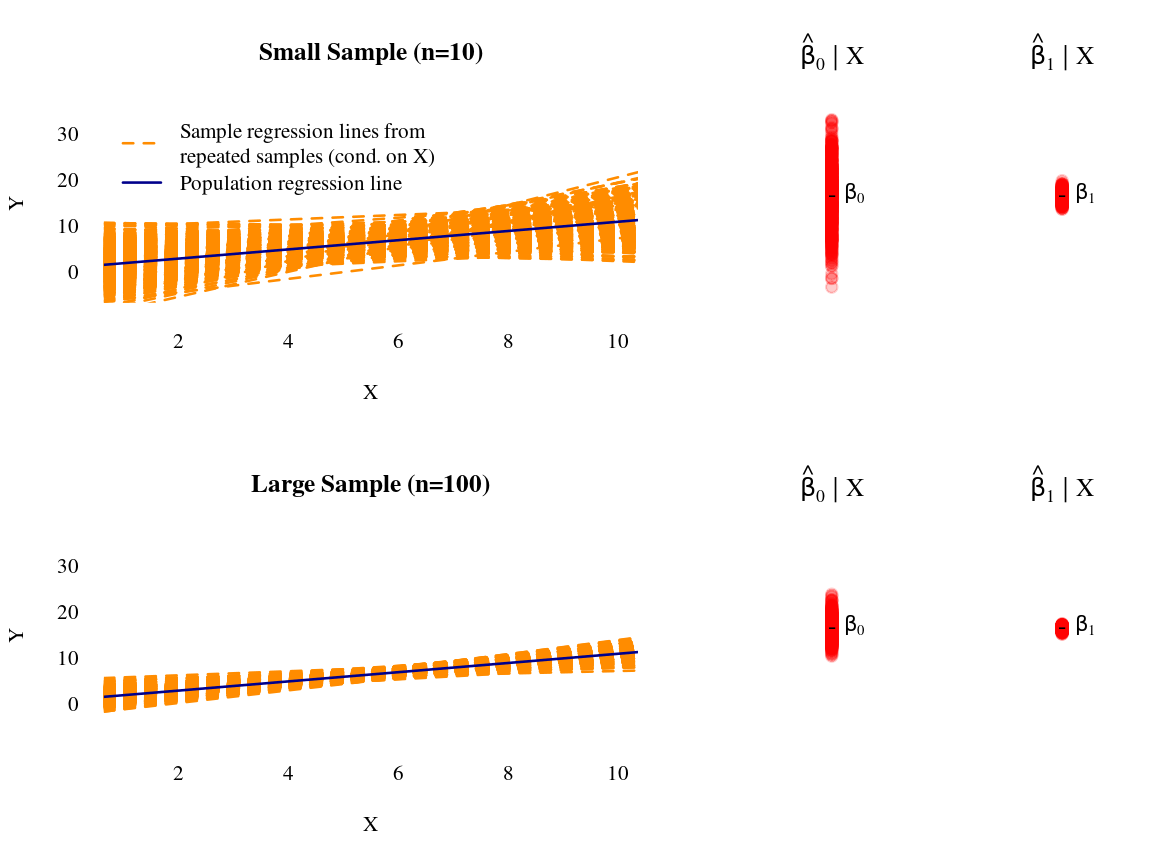
\includegraphics[width=\textwidth]{figure/minimal-unnamed-chunk-61-1} \end{center}

This are promising plots:

\begin{itemize}
\item The realizations of $\hat\beta_0|X$ and $\hat\beta_1|X$ are scattered around the true (unknown) parameter values $\beta_0$ and $\beta_1$ for both small and large samples.
\item The realizations of $\hat\beta_0|X$ and $\hat\beta_1|X$ concentrate more and more around the true (unknown) parameter values $\beta_0$ and $\beta_1$ as the sample size increases. 
\end{itemize}

However, this was only a simulation for one specific data generating process. Such a Monte Carlo simulation does not allow us to generalize these properties. Next we use theoretical arguments to show that these properties also hold in general.

\hypertarget{ch:SSINF}{%
\chapter{Small Sample Inference}\label{ch:SSINF}}

\paragraph*{Note on small sample sizes.}

Sometimes sample sizes of \(n<30\) are referred to as \say{small samples} since one often hopes that the central limit theorem is helping out for sample sizes \(n \geq 30\). However, this is a \text{very dangerous} rule of thumb! A sufficiently large \(n\) that allows us to rely on the central limit theorem depends on many different distributional aspects. In this chapter, we consider the case where we cannot rely on the central limit theorem.

\paragraph*{Exact inference.}

This chapter considers \emph{exact} inference using the multiple linear regression model. By \emph{exact} we mean correct distributions for each sample size \(n\). That is, no asymptotic (large \(n\to\infty\)) arguments will be used.

\paragraph*{Assumptions.}

Recall that we, in general, did not impose a complete distributional assumption on \(\eps\) in Assumption 4 -- the i.i.d. normal case in Assumption 4 was only one possible \emph{option}. However, to do exact inference, the normality Assumption on the error terms is not a mere option, but a \emph{necessity}. So for this chapter we assume that Assumptions 1-3 from Chapter \ref{ch:MLR} hold and that additionally the following assumption holds:

\paragraph*{Assumption $4^\ast$: Error distribution.}

For small sample cases, we assume that the error terms are
\textbf{i.i.d. normal}, i.e., \(\varepsilon_i\overset{\operatorname{i.i.d.}}{\sim}\mathcal{N}(0,\sigma^2)\) for all \(i=1,\dots,n\) which leads to spherical errors. That is,
\[
\eps\sim\mathcal{N}\left(0,\sigma^2I_n\right),
\]
where \(\eps=(\eps_1,\dots,\eps_n)'\).

\bigskip

\paragraph*{Normality of $\hat\beta$.}

Under Assumptions 1-4\(^\ast\) it can be shown that
\begin{align}
\hat\beta_n|X \sim \mathcal{N}\left(\beta,\V(\hat\beta_n|X)\right),\label{eq:ssnorm}
\end{align}
where \(\V(\hat\beta_n|X)=\sigma^2(X'X)^{-1}\).

This result follows from noting that \(\hat\beta_n=(X'X)^{-1}X'Y=\beta+(X'X)^{-1}X'\eps\) and because \((X'X)^{-1}X'\eps\) is just a linear combination of the normally distributed error terms \(\eps\) which, therefore, is again normally distributed, conditionally on \(X\). Note that \eqref{eq:ssnorm} is the \textit{exact} small sample distribution of \(\hat\beta_n|X\) and fully relies on the conditional normality assumption Assumption 4\(^*\).

\paragraph*{Note.}

The subscript \(n\) in \(\hat\beta_n\) is here only to emphasize that the distribution of \(\hat\beta_n\) depends on \(n\); we will, however, often simply write \(\hat\beta\).

\hypertarget{ch:testmultp}{%
\section{Hypothesis Tests about Multiple Parameters}\label{ch:testmultp}}

Let us consider the following system of \(q\)-many null hypotheses:
\begin{align*}
H_0: \underset{(q\times K)}{R}\underset{(K\times 1)}{\beta} - \underset{(q\times 1)}{r} = \underset{(q\times 1)}{0},
\end{align*}
where the \((q \times K)\) matrix \(R\) and the \(q\)-vector \(r=(r_{1},\dots,r_{q})'\) are chosen by the statistician to specify her/his null hypothesis about the unknown true parameter vector \(\beta\). To make sure that there are no redundant equations, it is required that \(\rank(R)=q\).

We must also specify the alternative against which we are testing the null hypothesis, for instance
\begin{equation*}
H_A: R\beta -r \neq 0
\end{equation*}

The above multiple parameter hypotheses cover also the special case of single parameter hypothesis; for instance, by setting \(R=(0,1,0\dots,0)\) and \(r=0\) one get's
\begin{equation*}
\begin{array}{ll}
H_0:  & \beta_{k}=0 \\
H_A:  & \beta_{k} \ne 0 \\
\end{array}
\end{equation*}

Under our assumptions (Assumptions 1 to 4\(^\ast\)), we have that
\[
(R\hat\beta_n-r)|X\sim\mathcal{N}\left(R\beta -r,R\V(\hat\beta_n|X)R'\right).
\]
So, the realizations of \((R\hat\beta_n -r)|X\) will scatter around the \emph{unknown} \((R\beta -r)\) in a non-systematical, Gaussian fashion. Therefore, if the null hypothesis is correct (i.e., \((R\beta-r)=0\)), the realizations of \((R\hat\beta_n-r)|X\) scatter around the \(q\)-vector \(0\). If, however, the alternative hypothesis is correct (i.e., \((R\beta-r)=a\neq 0\)), the realizations of \(R\hat\beta_n-r|X\) scatter around the \(q\)-vector \(a\neq 0\). So, under the alternative hypothesis, there will be a systematic location-shift of the \(q\)-dimensional random variable \(R\hat\beta_n|X\) away from \(r\) which we try to detect using statistical hypothesis testing.

\hypertarget{the-test-statistic-and-its-null-distribution}{%
\subsection{The Test Statistic and its Null Distribution}\label{the-test-statistic-and-its-null-distribution}}

The fact that \((R\hat\beta_n-r)\in\mathbb{R}^q\) is a \(q\)-dimensional random variable makes it a little bothersome to use as a test-statistic. Fortunately, we can turn \((R\hat\beta_n-r)\) into a scalar-valued test statistic using the following quadratic form:
\begin{align*}
W&=\underbrace{(R\hat\beta_n -r)'}_{(1\times q)}\underbrace{[R\V(\hat\beta_n|X)R']^{-1}}_{(q\times q)}\underbrace{(R\hat\beta_n -r)}_{(q\times 1)}
\end{align*}
Note that the test statistic \(W\) is simply measuring the distance (it's a weighted L2-distance) between the two \(q\)-vectors \(R\hat\beta_n\) and \(r\). Moreover, under the null hypothesis (i.e., if the null hypothesis is true), \(W\) is just a sum of \(q\)-many independent squared standard normal random variables. Therefore, under the null hypothesis, \(W\) is \(\chi^2(q)\) distributed with \(q\) degrees of freedom (see Section \ref{chisqdist}),
\begin{equation*}
W=(R\hat\beta_n -r)'[R\V(\hat\beta_n|X)R']^{-1}(R\hat\beta_n-r)\overset{H_0}{\sim} \chi^2(q).
\end{equation*}

Usually, we do not know \(\V(\hat\beta_n|X)\) and, therefore, have to estimate this quantity. Unfortunately, the general heteroscedasticity consistent robust estimators \(\widehat{\V_{\text{HC0}}}(\hat\beta_n|X)\), \(\dots\), \(\widehat{\V_{\text{HC4}}}(\hat\beta_n|X)\) from Chapter \ref{ch:MLR} are only asymptotically justified and, therefore, inappropriate for \emph{exact} small sample inference.

Thus, for truly \emph{exact} finite sample inference, we need a variance estimator for which we can derive the \emph{exact} small sample distribution. Therefore, we assume in Assumption 4\(^*\) spherical errors (i.e., \(\V(\eps|X)=I_n\sigma^2\)) which yield that \(\V(\hat\beta_n|X)=\sigma^2(X'X)^{-1}\), and where \(\sigma^2\) can be estimated by \(s_{UB}^2=(n-K)^{-1}\sum_{i=1}^n\hat\eps_i^2\). From the normality assumption in Assumption 4\(^*\), it follows then that \(\sigma^{-2}(n-K)s_{UB}^2\sim\chi^2(n-K)\). This then leads to the following exact null distribution of
\begin{align}\label{eq:Ftest}
F=(R\hat\beta_n -r)'[R(s_{UB}^2(X'X)^{-1})R']^{-1}(R\hat\beta_n -r)/q\overset{H_0}{\sim} F(q,n-K),
\end{align}
where \(F(q,n-K)\) denotes the \(F\)-distribution with \(q\) numerator and \(n-K\) denominator degrees of freedom \citep[see, for instance,][Ch. 1]{Hayashi2000}. By contrast to \(W\), \(F\) is a practically useful test-statistic, and we can use observed values \(F_{\text{obs}}\) to measure the distance of our estimate \(R\hat\beta_n\) from value \(r\). Observed values, \(F_{\text{obs}}\), that are unusually large under the null hypothesis, lead to a rejection of the null hypothesis. The null distribution \(F(q,n-K)\) of \(F\) is used to judge what's unusually large under the null hypothesis.

\paragraph*{The F distribution.}

The F distribution is a ratio of two \(\chi^2\) distributions. It has two parameters: the
numerator degrees of freedom, and the denominator degrees of freedom. Each
combination of the parameters yields a different F distribution. See Section \ref{sec:Fdist} for more information on the \(F\) statistic.

\begin{center}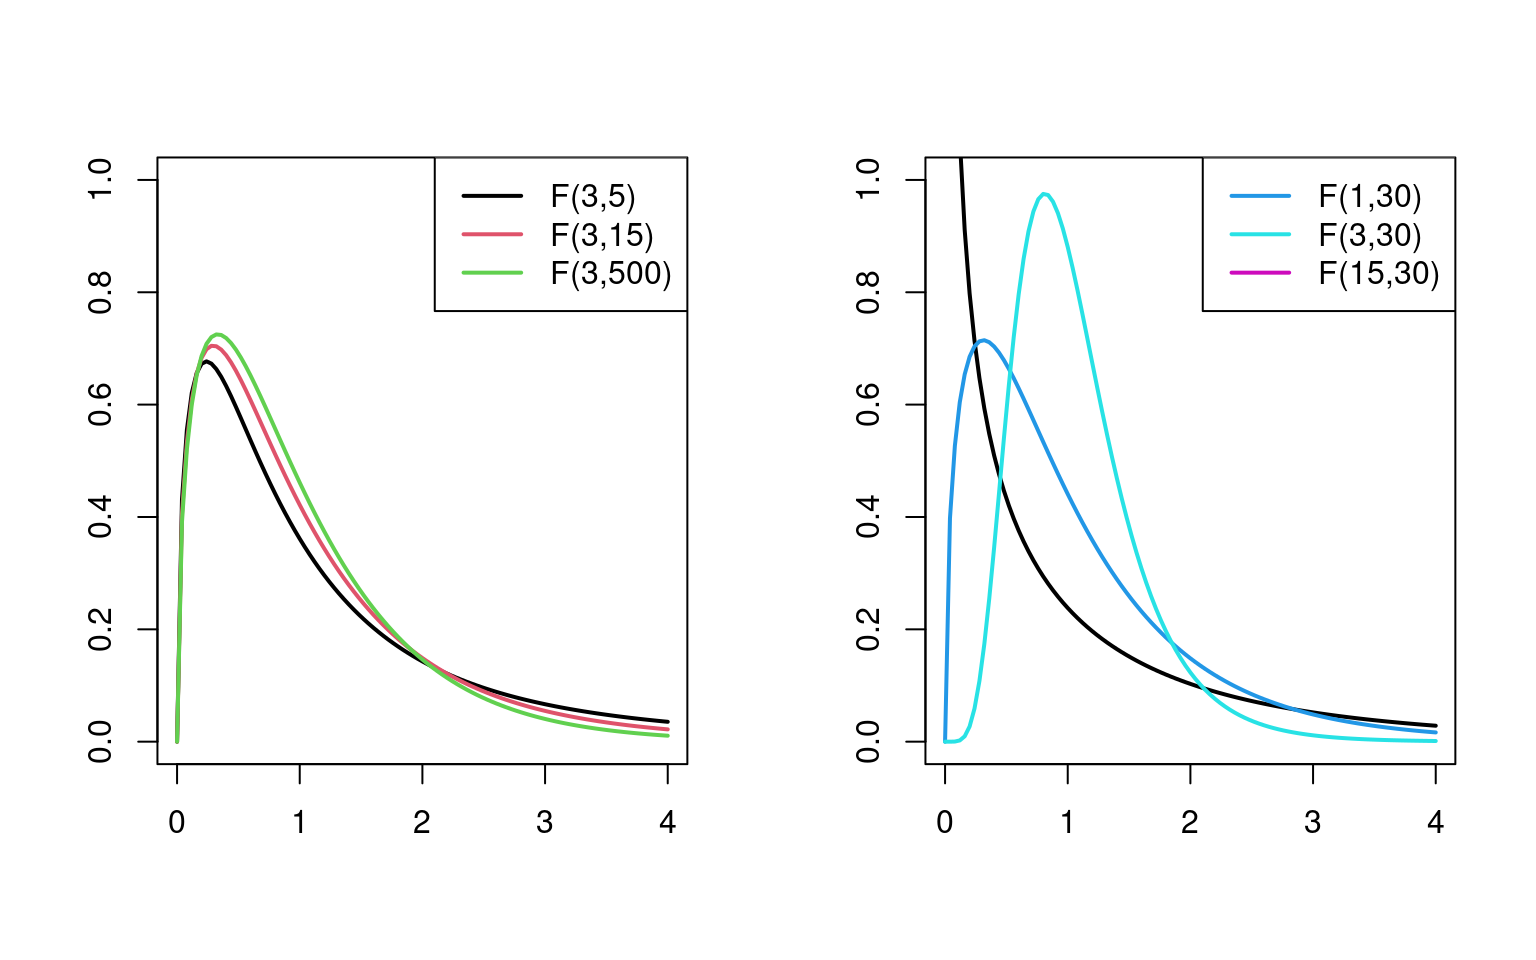
\includegraphics[width=1\textwidth]{figure/minimal-unnamed-chunk-62-1} \end{center}

\hypertarget{ch:testingsinglep}{%
\section{Tests about One Parameter}\label{ch:testingsinglep}}

For testing a hypothesis about only one parameter \(\beta_k\), with \(k=1,\dots,K\)
\begin{equation*}
\begin{array}{ll}
H_0: & \beta_k=r\\
H_A: & \beta_k\ne r\\
\end{array}
\end{equation*}
the (\(q\times K\)=\(1\times K\))-matrix \(R\) equals a row-vector of zeros but with a one as the \(k\)th element (e.g., for \(k=2\), \(R=(0,1,0,\dots,0)\)) such that \(F\) in \eqref{eq:Ftest} simplifies to
\[
\frac{\left(\hat{\beta}_k-r\right)^2}{\widehat{\V}(\hat{\beta}_k|X)}\overset{H_0}{\sim}F(1,n-K),
\]
where \(\widehat{\V}(\hat{\beta}_k|X)=R(s^2(X'X)^{-1})R'\). Taking square roots yields
\[
t=\frac{\hat{\beta}_k-r}{\widehat{\operatorname{SE}}(\hat{\beta}_k|X)}\overset{H_0}{\sim}t_{(n-K)}.
\]
Thus the \(t\)-distribution with \(n-K\) degrees of freedom is the appropriate reference metric for judging how ``far away'\,' our estimates are from the hypothetical parameter value \(r\) under the null hypothesis.

\paragraph*{Note.}

All commonly used statistical software packages report \(t\)-tests testing the null hypothesis \(H_0:\beta_k=0\), i.e., with \(r=0\). This means to test the null hypothesis that \(X_k\) has \say{no (linear) effect} on \(Y\).

The following plot illustrates that as the degrees of freedom increase, the shape of the \(t\) distribution comes closer to that of a standard normal bell curve. Already for \(25\) degrees of freedom we find little difference to the standard normal density. In case of small degrees of freedom values, we find the distribution to have heavier tails than a standard normal.

\begin{center}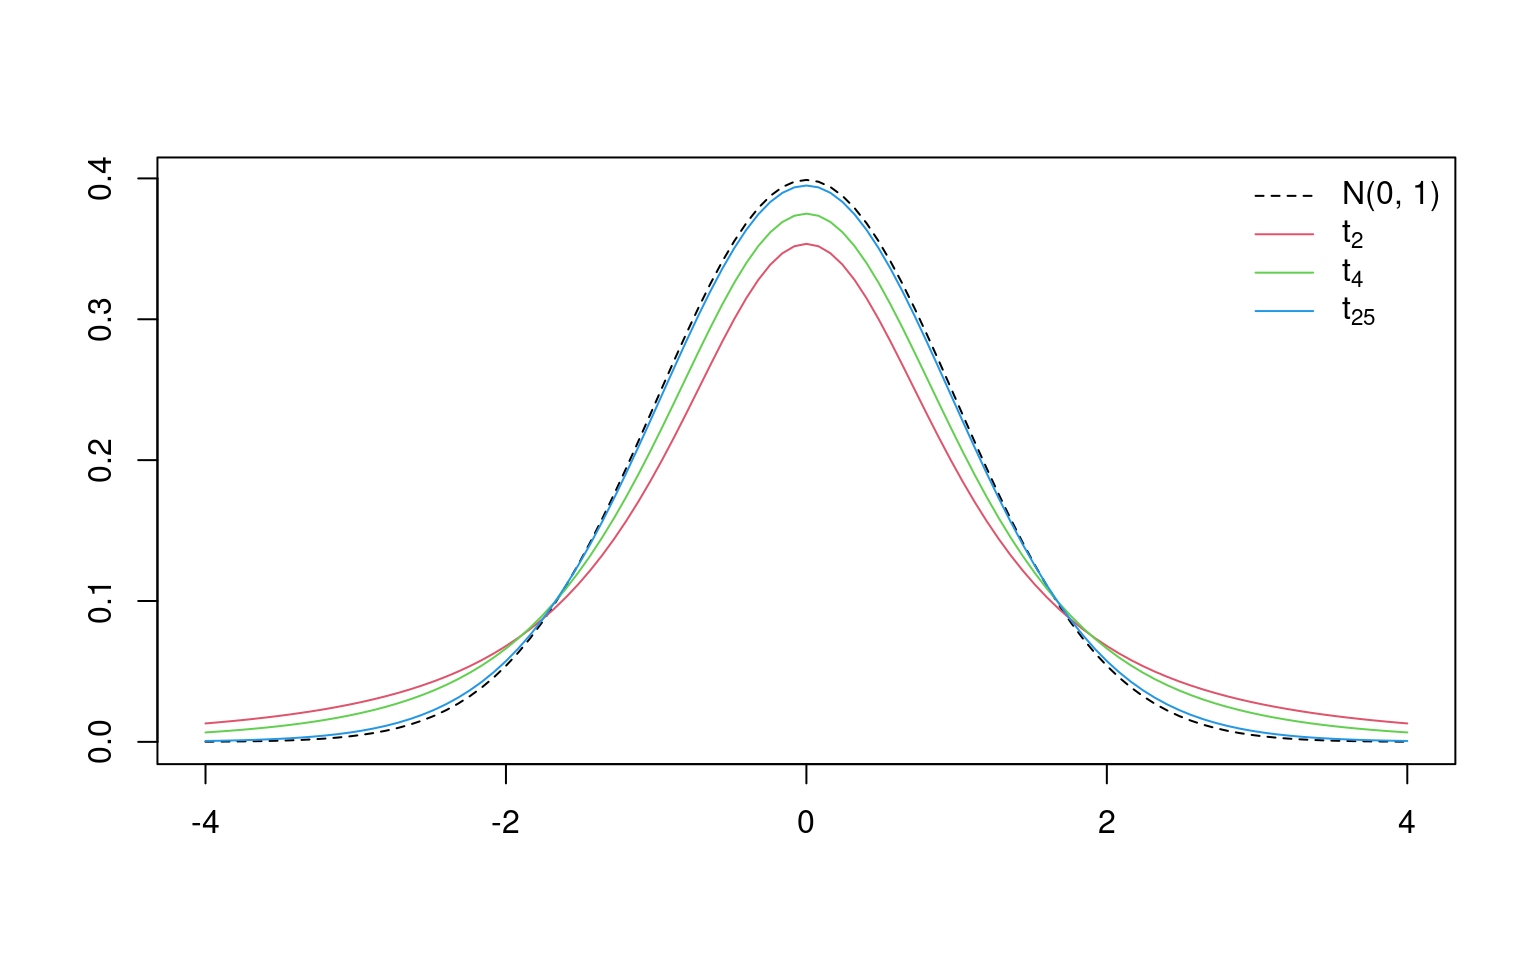
\includegraphics[width=1\textwidth]{figure/minimal-unnamed-chunk-63-1} \end{center}

\hypertarget{testtheory}{%
\section{Testtheory}\label{testtheory}}

\hypertarget{significance-level}{%
\subsection{Significance Level}\label{significance-level}}

To actually test the null hypothesis (e.g., H\(_0\): \(R\beta-r=0\) or \(H_0:\beta_k=0\)), we need to have a decision rule on when we will reject and not reject the null hypothesis. This amounts to deciding on a probability with which we are comfortable rejecting the null hypothesis when it is in fact true (Type I error or \(\alpha\) error). The probability of such a Type I error shall be bounded from above by a (small) significance level \(\alpha\), that is
\[
P(\text{reject } H_0| H_0\text{ is true})=P(\text{Type I Error})=\alpha
\]
For a given significance level (e.g., \(\alpha=0.05\)) and a given alternative hypothesis, we can divide the range of all possible values of the test statistic (i.e., \(\mathbb{R}\) since both \(t\in\mathbb{R}\) and \(F\in\mathbb{R}\)) into a \textbf{rejection region} and a \textbf{non-rejection region} by using certain quantiles called \textbf{critical values} of the test statistic distribution under the null. We can do this because the test statistics \(t\) and \(F\) have known distributions under the null hypothesis (\(t\overset{H_0}{\sim}t_{n-K}\) and \(F\overset{H_0}{\sim}F(q,n-K)\)); indeed, under Assumption 4\(^\ast\), we know the \emph{exact} null distributions for every sample size \(n\). Having decided on the rejection and non-rejection regions, it is a simple matter of seeing where the observed (obs) sample values \(t_{obs}\) or \(F_{obs}\) of the statistics \(t\) or \(F\) are--either in the rejection or in the non-rejection region.

\paragraph*{Non-conservative versus conservative tests.}

Since the test statistics \(F\) and \(t\) are continuous random variables of which we know the \emph{exact} distributions (under Assumptions 1-4\(^\ast\)), we can find critical values such that
\[
P(\text{Type I Error})=\alpha
\]
We call such tests \say{non-conservative} since the probability of a type I error equals the significance level \(\alpha\). Test statistics with
\[
P(\text{Type I Error})<\alpha
\]
are called \emph{conservative} test statistics; they lead to valid inferences, but will detect a violation of the null hypothesis less often than a non-conservative test. A test statistic with \(P(\text{Type I Error})>\alpha\) leads to \emph{invalid} inferences!

\hypertarget{critical-value-for-the-f-test}{%
\subsection{\texorpdfstring{Critical Value for the \(F\)-Test}{Critical Value for the F-Test}}\label{critical-value-for-the-f-test}}

The critical value \(c_{1-\alpha}>0\) defines the rejection region, \(]c_{1-\alpha},\infty[\), and non-rejection region, \(]0,c_{1-\alpha}]\) which divide the test-statistic space (here \(\mathbb{R}^+\) since \(F\in\mathbb{R}^+\)) for a given
significance level \(\alpha\in(0,1)\), such that
\[
P(\text{Type I Error})=P_{H_0}\Big(F\in]c_{1-\alpha},\infty[\Big)=\alpha,
\]
where \(c_{1-\alpha}\) is here the \((1-\alpha)\) quantile of the \(F\)-distribution with \((q,n-K)\) degrees of freedom, and where \(P_{H_0}\) means that we compute the probability under the assumption that \(H_0\) is true.

\begin{center}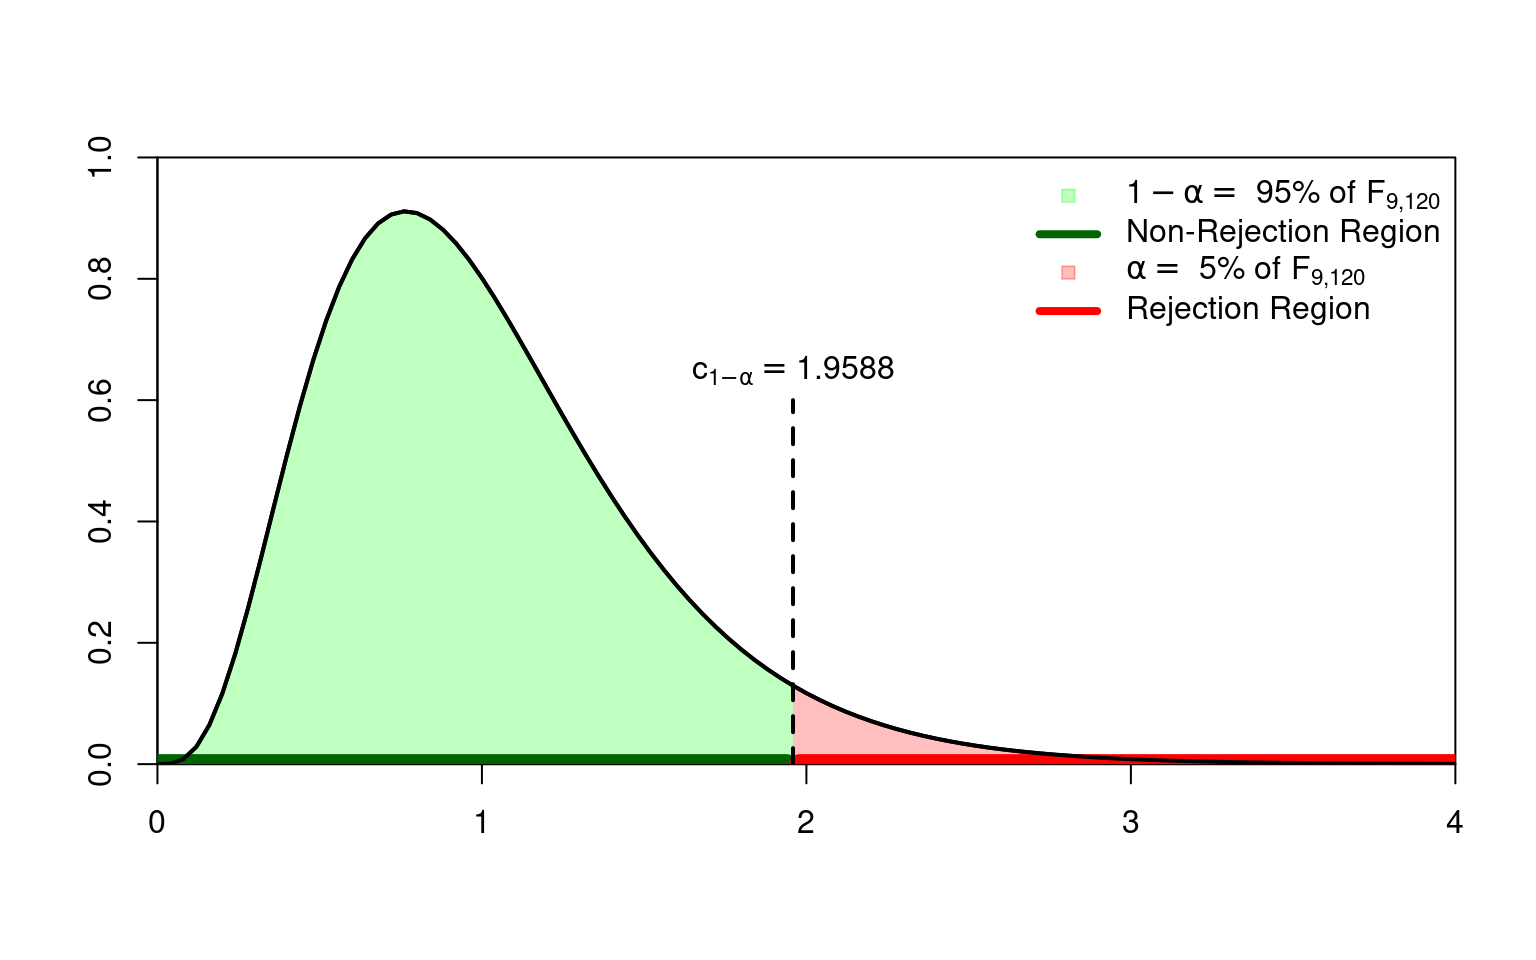
\includegraphics[width=1\textwidth]{figure/minimal-unnamed-chunk-64-1} \end{center}

\paragraph*{The rejection region.}

The rejection region describes a range of values of the test statistic \(F\) which we rarely see if the null hypothesis is true (only in at most \(\alpha \cdot 100\%\) cases). If the observed value of the test statistic, \(F_{\text{obs}}\), falls in this region, we will reject the null hypothesis--and hereby, accept Type I errors in at most \(\alpha \cdot 100\%\) of cases.

\paragraph*{The non-rejection region.}

The non-rejection region describes a range of values of the test statistic \(F\) which we expect to see (in \((1-\alpha) \cdot 100\%\) cases) if the null hypothesis is true. If the observed value of the test statistic, \(F_{\text{obs}}\) falls in this region, we will not reject the null hypothesis.

\paragraph*{Caution:}

Not rejecting the null hypothesis does not mean that we can conclude that the null hypothesis is true. We only had no sufficiently strong evidence against the null hypothesis. A violation of the null hypothesis, for instance \(R\beta -r=a\neq 0\), may simply be too small (too small \(a\) value) to stand out from the estimation errors (measured by the standard error) in \(\hat\beta_k\).

\paragraph*{Reading the $F$-Table.}

Fortunately, you do not need to read old-school distribution tables to find the critical value \(c_{1-\alpha}\), but can simply use \textsf{R}

\begin{Shaded}
\begin{Highlighting}[]
\NormalTok{df1   }\OtherTok{\textless{}{-}} \DecValTok{9}    \CommentTok{\# numerator df}
\NormalTok{df2   }\OtherTok{\textless{}{-}} \DecValTok{120}  \CommentTok{\# denominator df}
\NormalTok{alpha }\OtherTok{\textless{}{-}} \FloatTok{0.05} \CommentTok{\# significance level}
\DocumentationTok{\#\# Critical value:}
\NormalTok{crit\_value }\OtherTok{\textless{}{-}} \FunctionTok{qf}\NormalTok{(}\AttributeTok{p =} \DecValTok{1}\SpecialCharTok{{-}}\NormalTok{alpha, }\AttributeTok{df1 =}\NormalTok{ df1, }\AttributeTok{df2 =}\NormalTok{ df2)}
\NormalTok{crit\_value}
\CommentTok{\#\textgreater{} [1] 1.958763}
\end{Highlighting}
\end{Shaded}

\noindent Changing the significance level from \(\alpha=0.05\) to \(\alpha=0.01\) makes the critical value \(c_{1-\alpha}\) larger and, therefore, the rejection region smaller (fewer Type I errors)

\begin{Shaded}
\begin{Highlighting}[]
\NormalTok{alpha }\OtherTok{\textless{}{-}} \FloatTok{0.01}
\DocumentationTok{\#\# Critical value:}
\NormalTok{crit\_value }\OtherTok{\textless{}{-}} \FunctionTok{qf}\NormalTok{(}\AttributeTok{p =} \DecValTok{1}\SpecialCharTok{{-}}\NormalTok{alpha, }\AttributeTok{df1 =}\NormalTok{ df1, }\AttributeTok{df2 =}\NormalTok{ df2)}
\NormalTok{crit\_value}
\CommentTok{\#\textgreater{} [1] 2.558574}
\end{Highlighting}
\end{Shaded}

\hypertarget{critical-values-for-the-t-test}{%
\subsection{\texorpdfstring{Critical Value(s) for the \(t\)-Test}{Critical Value(s) for the t-Test}}\label{critical-values-for-the-t-test}}

In case of the \(t\)-test, we need to differentiate between two-sided and one-sided testing.

\hypertarget{two-sided-t-test}{%
\subsubsection*{\texorpdfstring{Two-Sided \(t\)-Test}{Two-Sided t-Test}}\label{two-sided-t-test}}
\addcontentsline{toc}{subsubsection}{Two-Sided \(t\)-Test}

Two-sided hypothesis:
\begin{equation*}
\begin{array}{ll}
H_0: & \beta_k=r \\
H_A: & \beta_k\ne r
\end{array}
\end{equation*}
In case of a two-sided \(t\)-test, we reject the null hypothesis if the observed realization of the \(t\)-test, \(t_{obs}\), is \say{far away} from zero either by being sufficiently smaller or greater than \(r\). The corresponding two-sided critical values are denoted by \(-c_{1-\alpha/2}=c_{\alpha/2}<0\) and \(c_{1-\alpha/2}>0\), where \(c_{1-\alpha/2}>0\) is the \((1-\alpha/2)\) quantile of the \(t\)-distribution with \((n-K)\) degrees of freedom, and where \(-c_{1-\alpha/2}=c_{\alpha/2}\) due to the symmetry of the \(t\)-distribution. These critical values defines the following rejection and the non-rejection regions
\begin{align*}
\text{rejection region:}&\hspace{1cm}]-\infty,c_{\alpha/2}[\;\;\cup\;\;]c_{1-\alpha/2}, \infty[\\
\text{non-rejection region:}&\hspace{1cm}[c_{\alpha/2},c_{1-\alpha/2}].
\end{align*}
For this rejection region it holds true that
\[
P(\text{Type I Error})=P_{H_0}\Big(t\in\;]-\infty,c_{\alpha/2}[\;\;\cup\;\;]c_{1-\alpha/2}, \infty[\Big)=\alpha.
\]

\begin{center}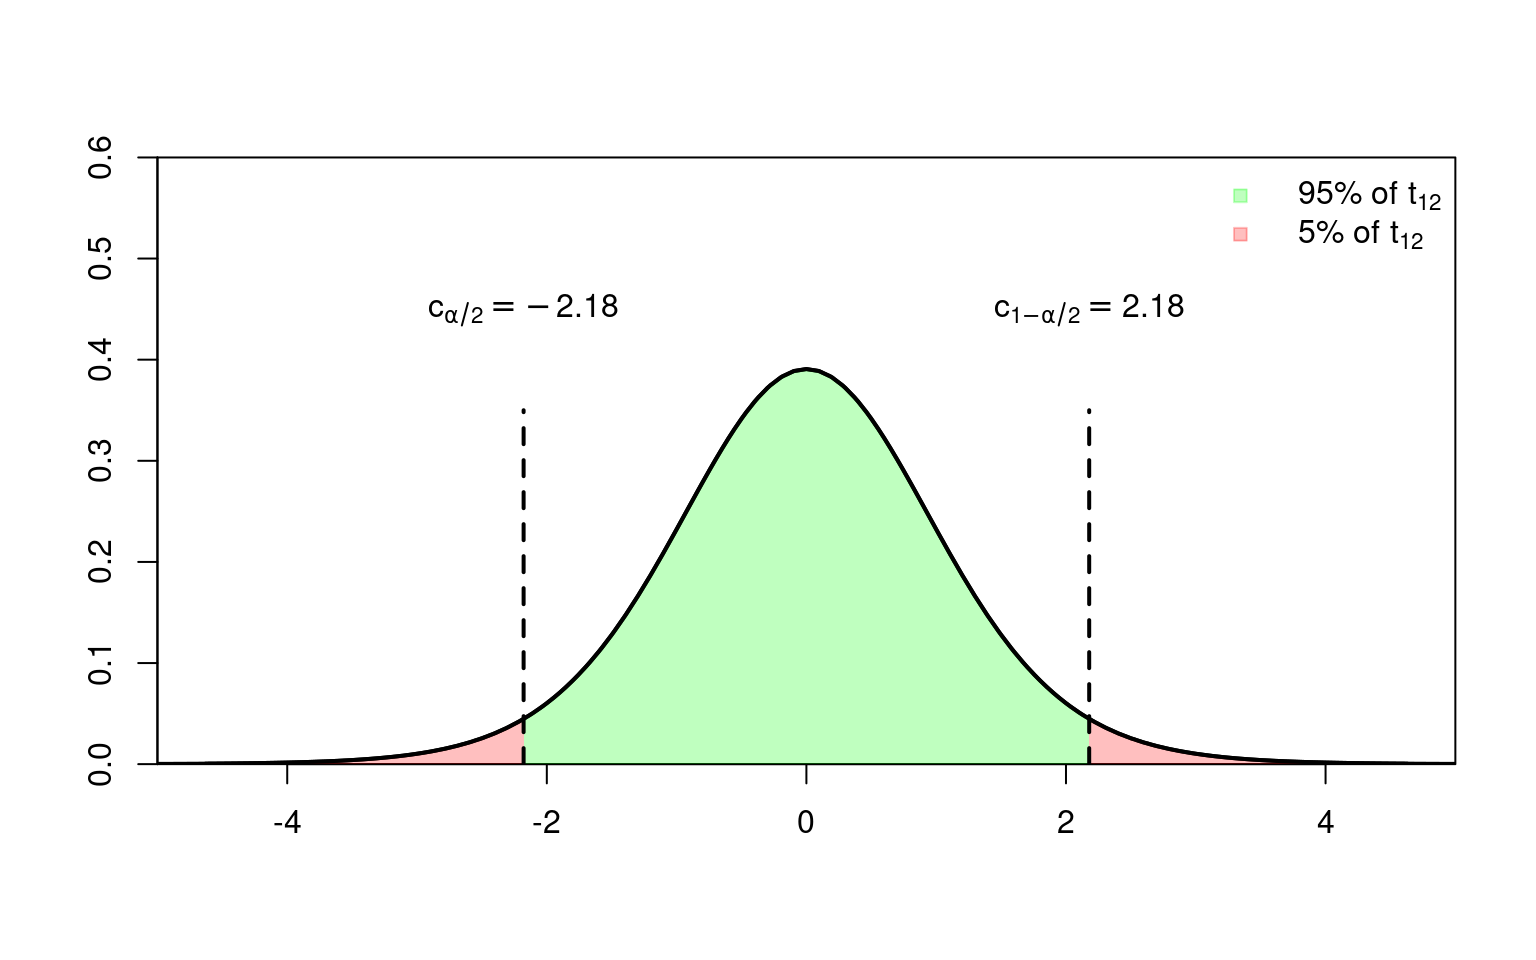
\includegraphics[width=1\textwidth]{figure/minimal-unnamed-chunk-67-1} \end{center}

\hypertarget{one-sided-t-test}{%
\subsubsection*{\texorpdfstring{One-Sided \(t\)-Test}{One-Sided t-Test}}\label{one-sided-t-test}}
\addcontentsline{toc}{subsubsection}{One-Sided \(t\)-Test}

One-sided hypothesis:
\begin{equation*}
\begin{array}{lll}
&H_0: & \beta_k =r\\
&H_A: & \beta_k >r\\
(\text{or}&H_A: & \beta_k< r)
\end{array}
\end{equation*}
In case of a one-sided \(t\)-test, we will reject the null if \(t_{obs}\) is sufficiently ``far away'\,' from zero in the relevant direction of \(H_A\). The corresponding critical value is either \(-c_{1-\alpha}\) (\(H_A:\beta_k< r\)) or \(c_{1-\alpha}\) (\(H_A:\beta_k> r\)), where \(c_{1-\alpha}\) is the \((1-\alpha)\) quantile of the \(t\)-distribution with \((n-K)\) degrees of freedom, and where \(-c_{1-\alpha}=c_{\alpha}\) due to the symmetry of the \(t\)-distribution. The critical value \(c_{1-\alpha}\) defines the following rejection and the non-rejection regions:

\bigskip

\noindent For \(H_0: \beta_k=0\) \quad versus\quad \(H_A: \beta_k < 0\):
\begin{align*}
\text{rejection region:}   &\hspace{2cm}]-\infty,c_{\alpha}[ \\
\text{non-rejection region:}&\hspace{2cm}[c_{\alpha},\infty[
\end{align*}
such that
\[
P(\text{Type I Error})=P_{H_0}\Big(t\in\;]-\infty,c_{\alpha}[\Big)=\alpha.
\]

\bigskip

\noindent For \(H_0: \beta_k=0\)\quad versus\quad\(H_A: \beta_k > 0\):
\begin{align*}
\text{rejection region:}&\hspace{1cm}]c_{1-\alpha}, \infty[\\
\text{non-rejection region:}&\hspace{1cm}]-\infty,c_{1-\alpha}]
\end{align*}
such that
\[
P(\text{Type I Error})=P_{H_0}\Big(t\in\;]c_{1-\alpha}, \infty[\Big)=\alpha.
\]

\begin{center}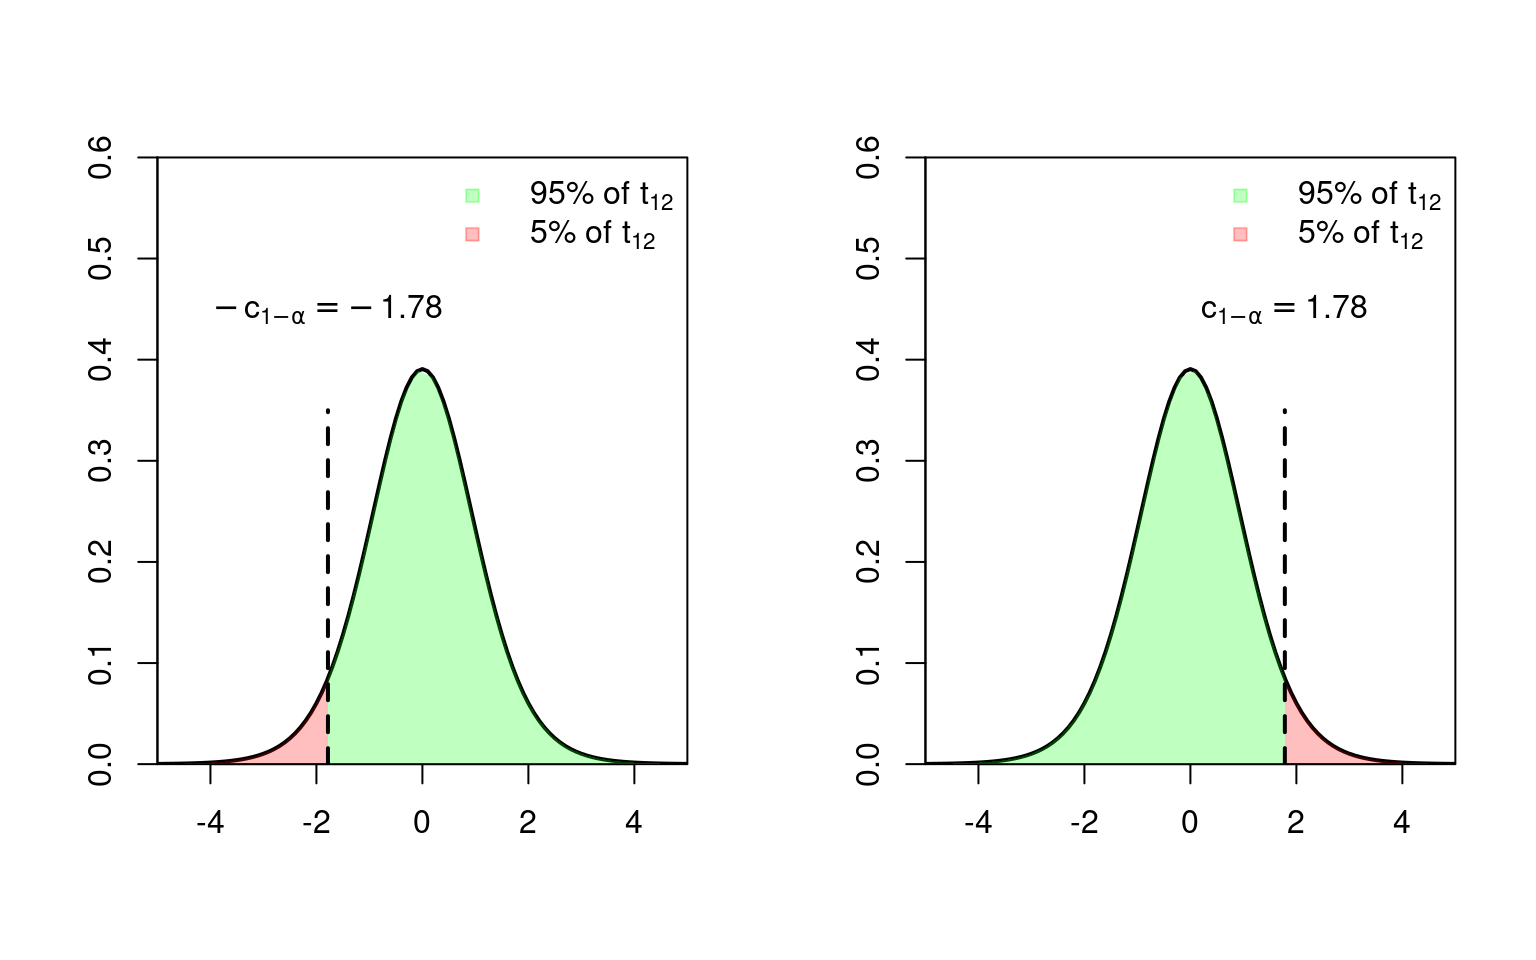
\includegraphics[width=1\textwidth]{figure/minimal-unnamed-chunk-68-1} \end{center}

\paragraph*{Reading the $t$-Table.}

Fortunately, you do not need to read old-school distribution tables to find the critical values, but you can simply use \textsf{R}

\begin{Shaded}
\begin{Highlighting}[]
\NormalTok{df    }\OtherTok{\textless{}{-}} \DecValTok{16}   \CommentTok{\# degrees of freedom }
\NormalTok{alpha }\OtherTok{\textless{}{-}} \FloatTok{0.05} \CommentTok{\# significance level}
\DocumentationTok{\#\# One{-}sided critical value (= (1{-}alpha) quantile):}
\NormalTok{c\_oneSided }\OtherTok{\textless{}{-}} \FunctionTok{qt}\NormalTok{(}\AttributeTok{p =} \DecValTok{1}\SpecialCharTok{{-}}\NormalTok{alpha, }\AttributeTok{df =}\NormalTok{ df)}
\NormalTok{c\_oneSided}
\CommentTok{\#\textgreater{} [1] 1.745884}
\DocumentationTok{\#\# Two{-}sided critical value (= (1{-}alpha/2) quantile):}
\NormalTok{c\_twoSided }\OtherTok{\textless{}{-}} \FunctionTok{qt}\NormalTok{(}\AttributeTok{p =} \DecValTok{1}\SpecialCharTok{{-}}\NormalTok{alpha}\SpecialCharTok{/}\DecValTok{2}\NormalTok{, }\AttributeTok{df =}\NormalTok{ df)}
\DocumentationTok{\#\# lower critical value}
\SpecialCharTok{{-}}\NormalTok{c\_twoSided}
\CommentTok{\#\textgreater{} [1] {-}2.119905}
\DocumentationTok{\#\# upper critical value}
\NormalTok{c\_twoSided}
\CommentTok{\#\textgreater{} [1] 2.119905}
\end{Highlighting}
\end{Shaded}

\hypertarget{type-ii-error-and-power}{%
\section{Type II Error and Power}\label{type-ii-error-and-power}}

A Type II error is the mistake of not rejecting the null hypothesis when in fact
it should have been rejected. The probability of making a Type II error equals one minus the probability of correctly rejecting the null hypothesis (\say{Power}). For instance, in the case of using the \(t\)-test to test the null hypothesis \(H_0: \beta_k=0\) versus the one-sided alternative hypothesis \(H_A:\beta_k>0\)) we have that
\begin{align*}
P(\text{Type II Error})
&=P_{H_A}\Big(t\;\in\;\overbrace{]-\infty,c_{1-\alpha}]}^{\text{non-rejection region}}\Big)\\
&=1-\underbrace{P_{H_A}\Big(t\;\in\;\overbrace{]c_{1-\alpha},\infty[}^{\text{rejection region}}\Big)}_{\text{\say{Power}}},
\end{align*}
where \(P_{H_A}\) means that we compute the probability under the assumption that \(H_A\) is true.

There is a trade off between the probability of making a Type I error and the probability of making a Type II error: a lower significance level \(\alpha\), decreases \(P(\text{Type I Error})\), but necessarily increases \(P(\text{Type II Error})\) and vice versa. Ideally, we would have some sense of the costs of making each of these errors, and would choose our significance level to minimize these total costs. However, the costs are often difficult to know. Moreover, the probability of making a Type II error is usually impossible to compute, since we usually do not know the true distribution of \(\hat\beta_k\) under the alternative.

For illustration purposes, however, consider the case of a \(t\) test for a one-sided hypothesis
\begin{equation*}
\begin{array}{ll}
H_0:  & \beta_k=0 \\
H_A:  & \beta_k>0,
\end{array}
\end{equation*}
where the true (usually unknown) parameter value is \(\beta_k=3\) and where the true (usually also unknown) standard error is \(\operatorname{SE}(\hat\beta_k|X)=\sqrt{\sigma^2[(X'X)^{-1}]_{kk}}=1.5\). The advantage here is that we can derive the distribution of the \(t\)-test statistic even under the alternative hypothesis. Note that the distribution of the \(t\)-test statistic becomes here a standard normal distribution, since we assume \(\operatorname{SE}(\hat\beta_k|X)=\sqrt{\sigma^2[(X'X)^{-1}]_{kk}}=1.5\) to be a \textbf{known} (deterministic) quantity. (This completely unrealistic assumption is only used for illustrative purposes!)

Under this setup, the distribution \say{under the null hypothesis} (i.e., if \(\beta_k=0\) were true) is:
\begin{align*}
t\big|X=\frac{\hat\beta_k}{\sqrt{\sigma^2[(X'X)^{-1}]_{kk}}}\Big|X\overset{H_0}{\sim}\mathcal{N}(0,1)
\end{align*}
Likewise, the distribution \say{under the alternative hypothesis} for the true parameter value (i.e., for the actual \(\beta_k=3\)) is:
\begin{align*}
t
=\frac{\hat\beta_k}{\sqrt{\sigma^2[(X'X)^{-1}]_{kk}}}
&=\frac{\hat\beta_k+3-3}{\sqrt{\sigma^2[(X'X)^{-1}]_{kk}}}\\[2ex]
\Rightarrow\quad&\underbrace{\frac{\hat\beta_k-3}{\sqrt{\sigma^2[(X'X)^{-1}]_{kk}}}}_{\substack{\sim \mathcal{N}(0,1)\\(\text{conditionally on $X$})}}+\underbrace{\frac{3}{\sqrt{\sigma^2[(X'X)^{-1}]_{kk}}}}_{=\Delta\text{ (mean-shift)}}\Big|X\overset{H_A}{\sim}\mathcal{N}(\Delta,1)
\end{align*}

So, the mean-shift \(\Delta\) depends on the value of \(\sqrt{\sigma^2[(X'X)^{-1}]_{kk}}\) and the difference between the actual parameter value (\(\beta_k=3\)) and the hypothetical parameter value under the null-hypothesis (here \(0\)). The following Graphic illustrates the probability of a type II error and the power for the case where \(\sqrt{\sigma^2[(X'X)^{-1}]_{kk}}=1.5\) such that \(\Delta=3/1.5=2\).

\begin{center}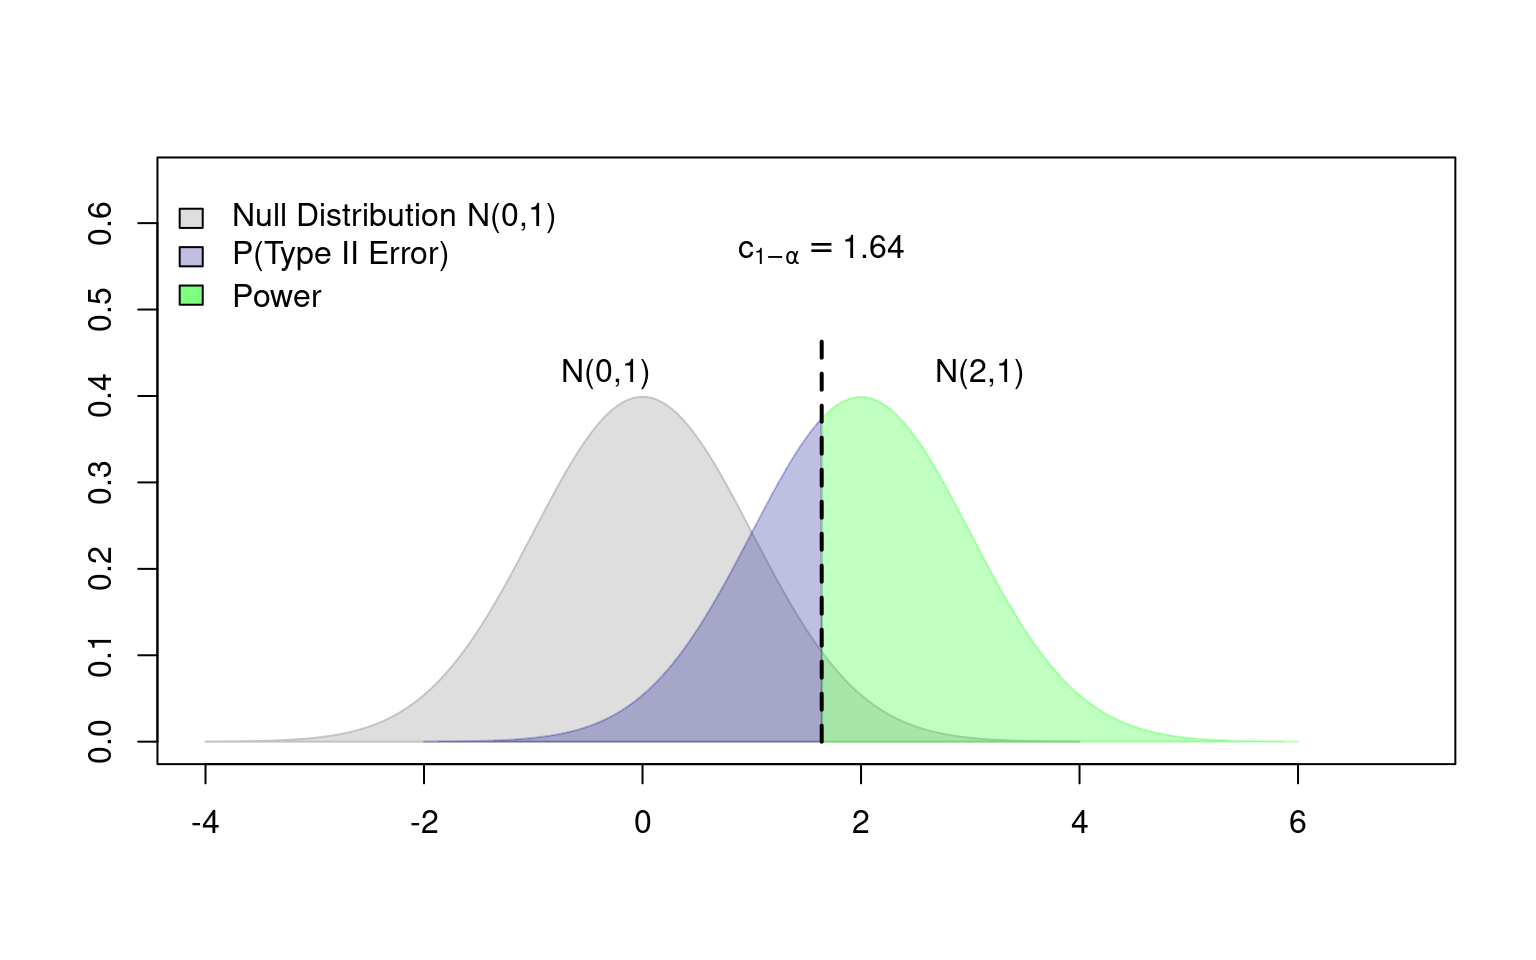
\includegraphics[width=1\textwidth]{figure/minimal-unnamed-chunk-70-1} \end{center}

\hypertarget{p-value}{%
\section{\texorpdfstring{\(p\)-Value}{p-Value}}\label{p-value}}

The \(p\)-value of a test statistic is the significance level we would obtain if we took the sample value of the observed test statistic, \(F_{\text{obs}}\) or \(t_{\text{obs}}\), as the border between the rejection and non-rejection regions.

\begin{description}
\item[$F$-test] $p=P_{H_0}(F\geq F_{\text{obs}})$
\item[$t$-test ($H_A:\beta_k\neq r$)] $p=2\cdot\min\{P_{H_0}(t\leq t_{\text{obs}}),P_{H_0}(t\geq t_{\text{obs}})\}$
\item[$t$-test ($H_A:\beta_k> r$)] $p=P_{H_0}(t\geq t_{\text{obs}})$
\item[$t$-test ($H_A:\beta_k< r$)] $p=P_{H_0}(t\leq t_{\text{obs}})$
\end{description}

Put another way, the \(p\)-value is the greatest significance level for which we just fail to reject the null. Therefore, the \(p\)-value is sometimes also called the marginal significance value.

If the \(p\)-value is strictly smaller than the chosen significance level \(\alpha\), we reject the null hypothesis.

\hypertarget{CIsmallsample}{%
\section{Confidence Intervals}\label{CIsmallsample}}

We define a two-sided \((1-\alpha)\cdot 100\%\) percent confidence interval for the \emph{deterministic} (unknown) true \(\beta_k\) as the \(\textbf{random interval}\) \(\operatorname{CI}_{1-\alpha}\) for which
\[
P\Big(\beta_k\in\operatorname{CI}_{1-\alpha}\Big)\geq 1-\alpha.
\]
Derivation of the \(\textbf{random interval}\) \(\operatorname{CI}_{1-\alpha}\): Observe that
\[
\frac{\hat\beta_k-\beta_k}{\widehat{\operatorname{SE}}(\hat\beta_k|X)}\sim t_{(n-K)}
\]
Therefore,
\begin{align*}
P\left(-t_{1-\alpha/2,n-K}\leq\frac{\hat\beta_k-\beta_k}{\widehat{\operatorname{SE}}(\hat\beta_k|X)}\leq t_{1-\alpha/2,n-K}\right)=1-\alpha,
\end{align*}
where \(t_{1-\alpha/2,n-K}\) denotes the \((1-\alpha)\) quantile of the \(t\)-distribution with \(n-K\) degrees of freedom. Next, we can do the following equivalent transformations
\begin{align*}
P\left(-t_{1-\alpha/2,n-K}\leq\frac{\hat\beta_k-\beta_k}{\widehat{\operatorname{SE}}(\hat\beta_k|X)}\leq t_{1-\alpha/2,n-K}\right)&=1-\alpha\\
\Leftrightarrow P\left(\hat\beta_k-t_{1-\alpha/2,n-K}\widehat{\operatorname{SE}}(\hat\beta_k|X)\leq \beta_k\leq\hat\beta_k +t_{1-\alpha/2,n-K}\widehat{\operatorname{SE}}(\hat\beta_k|X)\right)&=1-\alpha\\
\Leftrightarrow P\left(\beta_k\in\underbrace{\left[\hat\beta_k-t_{1-\alpha/2,n-K}\widehat{\operatorname{SE}}(\hat\beta_k|X),\;\hat\beta_k +t_{1-\alpha/2,n-K}\widehat{\operatorname{SE}}(\hat\beta_k|X)\right]}_{\operatorname{CI}_{1-\alpha}}\right)&=1-\alpha
\end{align*}
That is, the random interval
\[
\operatorname{CI}_{1-\alpha}=\left[\hat\beta_k-t_{1-\alpha/2,n-K}\widehat{\operatorname{SE}}(\hat\beta_k|X),\;\hat\beta_k +t_{1-\alpha/2,n-K}\widehat{\operatorname{SE}}(\hat\beta_k|X)\right]
\]
is our \((1-\alpha)\cdot 100\%\) percent confidence interval for \(\beta_k\).

\paragraph*{Interpretation.}

The random interval \(\operatorname{CI}_{1-\alpha}\) for \(\beta_k\) contains the true parameter value \(\beta_k\) in \((1-\alpha)\cdot 100\%\) cases of its realizations - when considering infinitely many realizations.\footnote{Take a look at this visualization: \url{https://rpsychologist.com/d3/ci/}} Unfortunately, this \say{interpretation} is not a statement about a single \(\operatorname{CI}_{1-\alpha}\) computed for given data. So, the problem with \(\operatorname{CI}\)s is that they are quite unintuitive. However, they are very well suited for a visual comparison of the estimation uncertainties in different parameter estimators, for instance, across \(\hat\beta_k\), \(k=1,\dots,K\).

\hypertarget{PSSI}{%
\section{Practice: Small Sample Inference}\label{PSSI}}

Let's apply the above exact inference methods using \textsf{R}. First, we program a function \texttt{myDataGenerator()} which allows us to generate data from the following model, i.e., from the following fully specified data generating process:
\begin{align*}
Y_i &=\beta_1+\beta_2X_{i2}+\beta_3X_{i3}+\eps_i,\qquad i=1,\dots,n\\
\beta &=(\beta_1,\beta_2,\beta_3)'=(2,3,4)'\\
X_{i2}&\sim U[2,10]\\
X_{i3}&\sim U[12,22]\\
\eps_i&\sim\mathcal{N}(0,3^2),
\end{align*}
where \((Y_i,X_i)\) is assumed i.i.d. across \(i=1,\dots,n\). Below, in the codes, I use \(n=10\), but, of course, other sample sizes can be considered too. Under the assumptions of this chapter, we do exact inference that is specific to any given sample size \(n\).

The below function \texttt{myDataGenerator()} allows to sample new realizations of \(Y_1,\dots,Y_n\) conditionally on a given data matrix \(X\). Moreover, you can provide your own values for the sample size \(n\) and for the parameter vector \(\beta=(\beta_1,\beta_2,\beta_3)'\).

\begin{Shaded}
\begin{Highlighting}[]
\DocumentationTok{\#\# Function to generate artificial data}
\DocumentationTok{\#\# If X=NULL: new X variables are generated}
\DocumentationTok{\#\# If the user gives X variables, }
\DocumentationTok{\#\# the sampling of new Y variables is conditionally on }
\DocumentationTok{\#\# the given X variables.}
\NormalTok{myDataGenerator }\OtherTok{\textless{}{-}} \ControlFlowTok{function}\NormalTok{(n, beta, }\AttributeTok{X=}\ConstantTok{NULL}\NormalTok{, }\AttributeTok{sigma=}\DecValTok{3}\NormalTok{)\{}
  \ControlFlowTok{if}\NormalTok{(}\FunctionTok{is.null}\NormalTok{(X))\{}
\NormalTok{    X   }\OtherTok{\textless{}{-}} \FunctionTok{cbind}\NormalTok{(}\FunctionTok{rep}\NormalTok{(}\DecValTok{1}\NormalTok{, n), }
                 \FunctionTok{runif}\NormalTok{(n, }\DecValTok{2}\NormalTok{, }\DecValTok{10}\NormalTok{), }
                 \FunctionTok{runif}\NormalTok{(n,}\DecValTok{12}\NormalTok{, }\DecValTok{22}\NormalTok{))}
\NormalTok{  \}}
\NormalTok{  eps  }\OtherTok{\textless{}{-}} \FunctionTok{rnorm}\NormalTok{(n, }\AttributeTok{sd=}\NormalTok{sigma)}
\NormalTok{  Y    }\OtherTok{\textless{}{-}}\NormalTok{ X }\SpecialCharTok{\%*\%}\NormalTok{ beta }\SpecialCharTok{+}\NormalTok{ eps}
\NormalTok{  data }\OtherTok{\textless{}{-}} \FunctionTok{data.frame}\NormalTok{(}\StringTok{"Y"}\OtherTok{=}\NormalTok{Y, }
                     \StringTok{"X\_1"}\OtherTok{=}\NormalTok{X[,}\DecValTok{1}\NormalTok{], }\StringTok{"X\_2"}\OtherTok{=}\NormalTok{X[,}\DecValTok{2}\NormalTok{], }\StringTok{"X\_3"}\OtherTok{=}\NormalTok{X[,}\DecValTok{3}\NormalTok{])}
  \DocumentationTok{\#\#}
  \FunctionTok{return}\NormalTok{(data)}
\NormalTok{\}}

\DocumentationTok{\#\# Define a true beta vector}
\NormalTok{beta\_true }\OtherTok{\textless{}{-}} \FunctionTok{c}\NormalTok{(}\DecValTok{2}\NormalTok{,}\DecValTok{3}\NormalTok{,}\DecValTok{4}\NormalTok{)}

\DocumentationTok{\#\# Check:}
\DocumentationTok{\#\# Generate Y and X data }
\NormalTok{test\_data     }\OtherTok{\textless{}{-}} \FunctionTok{myDataGenerator}\NormalTok{(}\AttributeTok{n =} \DecValTok{10}\NormalTok{, }\AttributeTok{beta=}\NormalTok{beta\_true)}
\DocumentationTok{\#\# Generate new Y data conditionally on X}
\NormalTok{X\_cond }\OtherTok{\textless{}{-}} \FunctionTok{cbind}\NormalTok{(test\_data}\SpecialCharTok{$}\NormalTok{X\_1,}
\NormalTok{                test\_data}\SpecialCharTok{$}\NormalTok{X\_2,}
\NormalTok{                test\_data}\SpecialCharTok{$}\NormalTok{X\_3)}
\NormalTok{test\_data\_new }\OtherTok{\textless{}{-}} \FunctionTok{myDataGenerator}\NormalTok{(}\AttributeTok{n    =} \DecValTok{10}\NormalTok{, }
                                 \AttributeTok{beta =}\NormalTok{ beta\_true, }
                                 \AttributeTok{X    =}\NormalTok{ X\_cond)}
\DocumentationTok{\#\# compare}
\FunctionTok{round}\NormalTok{(}\FunctionTok{head}\NormalTok{(test\_data,     }\DecValTok{3}\NormalTok{), }\DecValTok{2}\NormalTok{) }\CommentTok{\# New Y, new X}
\CommentTok{\#\textgreater{}       Y X\_1  X\_2   X\_3}
\CommentTok{\#\textgreater{} 1 89.36   1 4.04 19.62}
\CommentTok{\#\textgreater{} 2 96.87   1 8.19 17.55}
\CommentTok{\#\textgreater{} 3 88.71   1 2.81 20.34}
\FunctionTok{round}\NormalTok{(}\FunctionTok{head}\NormalTok{(test\_data\_new, }\DecValTok{3}\NormalTok{), }\DecValTok{2}\NormalTok{) }\CommentTok{\# New Y, conditionally on X}
\CommentTok{\#\textgreater{}       Y X\_1  X\_2   X\_3}
\CommentTok{\#\textgreater{} 1 96.06   1 4.04 19.62}
\CommentTok{\#\textgreater{} 2 95.72   1 8.19 17.55}
\CommentTok{\#\textgreater{} 3 94.02   1 2.81 20.34}
\end{Highlighting}
\end{Shaded}

\hypertarget{normally-distributed-hatbetax}{%
\subsection{\texorpdfstring{Normally Distributed \(\hat\beta|X\)}{Normally Distributed \textbackslash hat\textbackslash beta\textbar X}}\label{normally-distributed-hatbetax}}

The above data generating process fulfills our regulatory assumptions Assumption 1-4\(^*\). So, by theory, the estimators \(\hat\beta_k|X\) should be normal distributed conditionally on \(X\)
\[
\hat\beta_k|X\sim\mathcal{N}(\beta_k,\sigma^2[(X'X)^{-1}]_{kk})
\]
where \([(X'X)^{-1}]_{kk}\) denotes the element in the \(k\)th row and \(k\)th column of the matrix \((X'X)^{-1}\). Let's check the distribution by means of a Monte Carlo simulation for the case of \(\hat\beta_2|X\) with a small sample size of \(n=10\).

\begin{Shaded}
\begin{Highlighting}[]
\FunctionTok{set.seed}\NormalTok{(}\DecValTok{123}\NormalTok{)}
\NormalTok{n         }\OtherTok{\textless{}{-}} \DecValTok{10}       \CommentTok{\# a small sample size}
\NormalTok{beta\_true }\OtherTok{\textless{}{-}} \FunctionTok{c}\NormalTok{(}\DecValTok{2}\NormalTok{,}\DecValTok{3}\NormalTok{,}\DecValTok{4}\NormalTok{) }\CommentTok{\# true data vector}
\NormalTok{sigma     }\OtherTok{\textless{}{-}} \DecValTok{3}        \CommentTok{\# true standard deviation of the error term (var=sigma\^{}2)}

\DocumentationTok{\#\# Let\textquotesingle{}s generate a data set from our data generating process}
\NormalTok{mydata  }\OtherTok{\textless{}{-}} \FunctionTok{myDataGenerator}\NormalTok{(}\AttributeTok{n =}\NormalTok{ n, }\AttributeTok{beta=}\NormalTok{beta\_true)}
\NormalTok{X\_cond  }\OtherTok{\textless{}{-}} \FunctionTok{cbind}\NormalTok{(mydata}\SpecialCharTok{$}\NormalTok{X\_1, mydata}\SpecialCharTok{$}\NormalTok{X\_2, mydata}\SpecialCharTok{$}\NormalTok{X\_3)}

\DocumentationTok{\#\# True mean and variance of the true normal distribution }
\DocumentationTok{\#\# of beta\_hat\_2|X=X\_cond:}
\CommentTok{\# true mean}
\NormalTok{beta\_true\_2     }\OtherTok{\textless{}{-}}\NormalTok{ beta\_true[}\DecValTok{2}\NormalTok{] }
\CommentTok{\# true variance}
\NormalTok{var\_true\_beta\_2 }\OtherTok{\textless{}{-}}\NormalTok{ sigma}\SpecialCharTok{\^{}}\DecValTok{2} \SpecialCharTok{*} \FunctionTok{diag}\NormalTok{(}\FunctionTok{solve}\NormalTok{(}\FunctionTok{t}\NormalTok{(X\_cond) }\SpecialCharTok{\%*\%}\NormalTok{ X\_cond))[}\DecValTok{2}\NormalTok{]}

\DocumentationTok{\#\# Let\textquotesingle{}s generate 5000 realizations from beta\_hat\_2 }
\DocumentationTok{\#\# conditionally on X=X\_cond and check whether the empirical  }
\DocumentationTok{\#\# distribution of these 5000 realizations is close }
\DocumentationTok{\#\# to the true normal distribution of beta\_hat\_2:}
\NormalTok{rep        }\OtherTok{\textless{}{-}} \DecValTok{5000} \CommentTok{\# MC replications}
\NormalTok{beta\_hat\_2 }\OtherTok{\textless{}{-}} \FunctionTok{rep}\NormalTok{(}\ConstantTok{NA}\NormalTok{, }\AttributeTok{times=}\NormalTok{rep)}
\DocumentationTok{\#\#}
\ControlFlowTok{for}\NormalTok{(r }\ControlFlowTok{in} \DecValTok{1}\SpecialCharTok{:}\NormalTok{rep)\{}
\NormalTok{    MC\_data }\OtherTok{\textless{}{-}} \FunctionTok{myDataGenerator}\NormalTok{(}\AttributeTok{n    =}\NormalTok{ n, }
                               \AttributeTok{beta =}\NormalTok{ beta\_true, }
                               \AttributeTok{X    =}\NormalTok{ X\_cond)}
\NormalTok{    lm\_obj        }\OtherTok{\textless{}{-}} \FunctionTok{lm}\NormalTok{(Y }\SpecialCharTok{\textasciitilde{}}\NormalTok{ X\_2 }\SpecialCharTok{+}\NormalTok{ X\_3, }\AttributeTok{data =}\NormalTok{ MC\_data)}
\NormalTok{    beta\_hat\_2[r] }\OtherTok{\textless{}{-}} \FunctionTok{coef}\NormalTok{(lm\_obj)[}\DecValTok{2}\NormalTok{]}
\NormalTok{\}}

\DocumentationTok{\#\# Compare}
\DocumentationTok{\#\# True beta\_2 versus average of beta\_hat\_2 estimates}
\NormalTok{beta\_true\_2}
\CommentTok{\#\textgreater{} [1] 3}
\FunctionTok{round}\NormalTok{(}\FunctionTok{mean}\NormalTok{(beta\_hat\_2), }\DecValTok{4}\NormalTok{)}
\CommentTok{\#\textgreater{} [1] 3.0091}
\DocumentationTok{\#\# True variance of beta\_hat\_2 versus }
\DocumentationTok{\#\# empirical variance of beta\_hat\_2 estimates}
\FunctionTok{round}\NormalTok{(var\_true\_beta\_2, }\DecValTok{4}\NormalTok{)}
\CommentTok{\#\textgreater{} [1] 0.416}
\FunctionTok{round}\NormalTok{(}\FunctionTok{var}\NormalTok{(beta\_hat\_2), }\DecValTok{4}\NormalTok{)}
\CommentTok{\#\textgreater{} [1] 0.4235}

\DocumentationTok{\#\# True normal distribution of beta\_hat\_2 versus }
\DocumentationTok{\#\# empirical density of beta\_hat\_2 estimates}
\FunctionTok{library}\NormalTok{(}\StringTok{"scales"}\NormalTok{)}
\FunctionTok{curve}\NormalTok{(}\AttributeTok{expr =} \FunctionTok{dnorm}\NormalTok{(x, }\AttributeTok{mean =}\NormalTok{ beta\_true\_2, }
                   \AttributeTok{sd=}\FunctionTok{sqrt}\NormalTok{(var\_true\_beta\_2)), }
      \AttributeTok{xlab=}\StringTok{""}\NormalTok{,}\AttributeTok{ylab=}\StringTok{""}\NormalTok{, }\AttributeTok{col=}\FunctionTok{gray}\NormalTok{(.}\DecValTok{2}\NormalTok{), }\AttributeTok{lwd=}\DecValTok{3}\NormalTok{, }\AttributeTok{lty=}\DecValTok{1}\NormalTok{, }
      \AttributeTok{xlim=}\FunctionTok{range}\NormalTok{(beta\_hat\_2), }\AttributeTok{ylim=}\FunctionTok{c}\NormalTok{(}\DecValTok{0}\NormalTok{,}\FloatTok{1.1}\NormalTok{))}
\FunctionTok{hist}\NormalTok{(beta\_hat\_2, }\AttributeTok{freq=}\ConstantTok{FALSE}\NormalTok{, }\AttributeTok{col=}\FunctionTok{alpha}\NormalTok{(}\StringTok{"blue"}\NormalTok{,.}\DecValTok{35}\NormalTok{), }\AttributeTok{add=}\ConstantTok{TRUE}\NormalTok{)}
\FunctionTok{lines}\NormalTok{(}\FunctionTok{density}\NormalTok{(beta\_hat\_2, }\AttributeTok{bw =} \FunctionTok{bw.SJ}\NormalTok{(beta\_hat\_2)), }
      \AttributeTok{col=}\FunctionTok{alpha}\NormalTok{(}\StringTok{"blue"}\NormalTok{,.}\DecValTok{5}\NormalTok{), }\AttributeTok{lwd=}\DecValTok{3}\NormalTok{)}
\FunctionTok{legend}\NormalTok{(}\StringTok{"topleft"}\NormalTok{, }\AttributeTok{lty=}\FunctionTok{c}\NormalTok{(}\DecValTok{1}\NormalTok{,}\ConstantTok{NA}\NormalTok{,}\DecValTok{1}\NormalTok{), }\AttributeTok{lwd=}\FunctionTok{c}\NormalTok{(}\DecValTok{3}\NormalTok{,}\ConstantTok{NA}\NormalTok{,}\DecValTok{3}\NormalTok{), }\AttributeTok{pch=}\FunctionTok{c}\NormalTok{(}\ConstantTok{NA}\NormalTok{,}\DecValTok{15}\NormalTok{,}\ConstantTok{NA}\NormalTok{), }\AttributeTok{pt.cex=}\FunctionTok{c}\NormalTok{(}\ConstantTok{NA}\NormalTok{,}\DecValTok{2}\NormalTok{,}\ConstantTok{NA}\NormalTok{),}
     \AttributeTok{col=}\FunctionTok{c}\NormalTok{(}\FunctionTok{gray}\NormalTok{(.}\DecValTok{2}\NormalTok{), }\FunctionTok{alpha}\NormalTok{(}\StringTok{"blue"}\NormalTok{,.}\DecValTok{45}\NormalTok{), }\FunctionTok{alpha}\NormalTok{(}\StringTok{"blue"}\NormalTok{,.}\DecValTok{5}\NormalTok{)), }\AttributeTok{bty=}\StringTok{"n"}\NormalTok{, }\AttributeTok{legend=} 
\FunctionTok{c}\NormalTok{(}\FunctionTok{expression}\NormalTok{(}
  \StringTok{"Theoretical Gaussian Density of"}\SpecialCharTok{\textasciitilde{}}\FunctionTok{hat}\NormalTok{(beta)[}\DecValTok{2}\NormalTok{]}\SpecialCharTok{\textasciitilde{}}\StringTok{\textquotesingle{}|\textquotesingle{}}\SpecialCharTok{\textasciitilde{}}\NormalTok{X), }
  \FunctionTok{expression}\NormalTok{(}
  \StringTok{"Histogram based on the 5000 MC realizations of"}\SpecialCharTok{\textasciitilde{}}
  \FunctionTok{hat}\NormalTok{(beta)[}\DecValTok{2}\NormalTok{]}\SpecialCharTok{\textasciitilde{}}\StringTok{\textquotesingle{}|\textquotesingle{}}\SpecialCharTok{\textasciitilde{}}\NormalTok{X), }
  \FunctionTok{expression}\NormalTok{(}
  \StringTok{"Nonparametric Density Estimation based on the 5000 MC realizations of"}\SpecialCharTok{\textasciitilde{}}
  \FunctionTok{hat}\NormalTok{(beta)[}\DecValTok{2}\NormalTok{]}\SpecialCharTok{\textasciitilde{}}\StringTok{\textquotesingle{}|\textquotesingle{}}\SpecialCharTok{\textasciitilde{}}\NormalTok{X)))}
\end{Highlighting}
\end{Shaded}

\begin{center}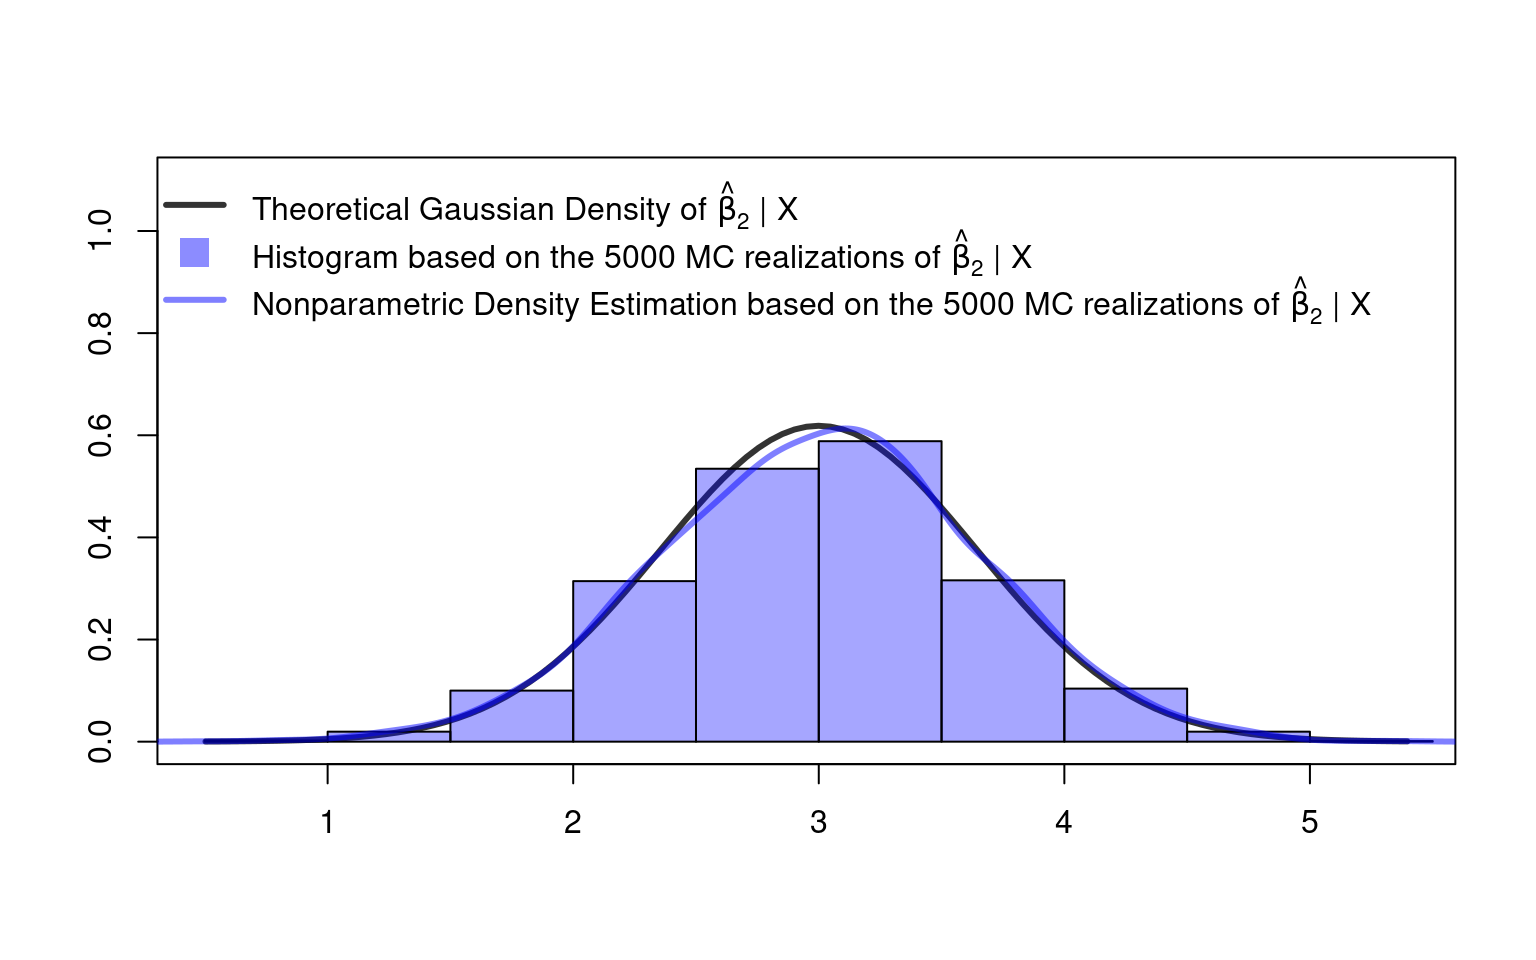
\includegraphics[width=1\textwidth]{figure/minimal-unnamed-chunk-72-1} \end{center}

Great! The nonparametric density estimation (estimated via \texttt{density()}) and the histogram computed based on the 5000 simulated realizations of \(\hat\beta_2|X\) are indicating that \(\hat\beta_2|X\) is really normally distributed as described by our theoretical result in Equation \eqref{eq:ssnorm}.

However, what would happen if we would sample \emph{unconditionally} on \(X\)? How does the distribution of \(\hat\beta_2\) would then look like?

\begin{Shaded}
\begin{Highlighting}[]
\FunctionTok{set.seed}\NormalTok{(}\DecValTok{123}\NormalTok{)}
\DocumentationTok{\#\# Let\textquotesingle{}s generate 5000 realizations from beta\_hat\_2 }
\DocumentationTok{\#\# WITHOUT conditioning on X}
\NormalTok{beta\_hat\_2\_uncond }\OtherTok{\textless{}{-}} \FunctionTok{rep}\NormalTok{(}\ConstantTok{NA}\NormalTok{, }\AttributeTok{times=}\NormalTok{rep)}
\DocumentationTok{\#\#}
\ControlFlowTok{for}\NormalTok{(r }\ControlFlowTok{in} \DecValTok{1}\SpecialCharTok{:}\NormalTok{rep)\{}
\NormalTok{    MC\_data }\OtherTok{\textless{}{-}} \FunctionTok{myDataGenerator}\NormalTok{(}\AttributeTok{n    =}\NormalTok{ n, }
                               \AttributeTok{beta =}\NormalTok{ beta\_true)}
\NormalTok{    lm\_obj               }\OtherTok{\textless{}{-}} \FunctionTok{lm}\NormalTok{(Y }\SpecialCharTok{\textasciitilde{}}\NormalTok{ X\_2 }\SpecialCharTok{+}\NormalTok{ X\_3, }\AttributeTok{data =}\NormalTok{ MC\_data)}
\NormalTok{    beta\_hat\_2\_uncond[r] }\OtherTok{\textless{}{-}} \FunctionTok{coef}\NormalTok{(lm\_obj)[}\DecValTok{2}\NormalTok{]}
\NormalTok{\}}

\DocumentationTok{\#\# Compare}
\DocumentationTok{\#\# True beta\_2 versus average of beta\_hat\_2 estimates}
\NormalTok{beta\_true\_2}
\CommentTok{\#\textgreater{} [1] 3}
\FunctionTok{round}\NormalTok{(}\FunctionTok{mean}\NormalTok{(beta\_hat\_2\_uncond), }\DecValTok{4}\NormalTok{)}
\CommentTok{\#\textgreater{} [1] 2.9973}
\DocumentationTok{\#\# True variance of beta\_hat\_2 versus }
\DocumentationTok{\#\# empirical variance of beta\_hat\_2 estimates}
\FunctionTok{round}\NormalTok{(var\_true\_beta\_2, }\DecValTok{4}\NormalTok{)}
\CommentTok{\#\textgreater{} [1] 0.416}
\FunctionTok{round}\NormalTok{(}\FunctionTok{var}\NormalTok{(beta\_hat\_2\_uncond), }\DecValTok{4}\NormalTok{)}
\CommentTok{\#\textgreater{} [1] 0.2521}

\DocumentationTok{\#\# Plot}
\FunctionTok{curve}\NormalTok{(}\AttributeTok{expr =} \FunctionTok{dnorm}\NormalTok{(x, }\AttributeTok{mean =}\NormalTok{ beta\_true\_2, }
                   \AttributeTok{sd=}\FunctionTok{sqrt}\NormalTok{(var\_true\_beta\_2)), }
      \AttributeTok{xlab=}\StringTok{""}\NormalTok{,}\AttributeTok{ylab=}\StringTok{""}\NormalTok{, }\AttributeTok{col=}\FunctionTok{gray}\NormalTok{(.}\DecValTok{2}\NormalTok{), }\AttributeTok{lwd=}\DecValTok{3}\NormalTok{, }\AttributeTok{lty=}\DecValTok{1}\NormalTok{, }
      \AttributeTok{xlim=}\FunctionTok{range}\NormalTok{(beta\_hat\_2\_uncond), }\AttributeTok{ylim=}\FunctionTok{c}\NormalTok{(}\DecValTok{0}\NormalTok{,}\FloatTok{1.5}\NormalTok{))}
\FunctionTok{hist}\NormalTok{(beta\_hat\_2\_uncond, }\AttributeTok{freq=}\ConstantTok{FALSE}\NormalTok{, }\AttributeTok{col=}\FunctionTok{alpha}\NormalTok{(}\StringTok{"blue"}\NormalTok{,.}\DecValTok{35}\NormalTok{), }\AttributeTok{add=}\ConstantTok{TRUE}\NormalTok{)}
\FunctionTok{lines}\NormalTok{(}\FunctionTok{density}\NormalTok{(beta\_hat\_2\_uncond, }\AttributeTok{bw=}\FunctionTok{bw.SJ}\NormalTok{(beta\_hat\_2\_uncond)), }
      \AttributeTok{col=}\FunctionTok{alpha}\NormalTok{(}\StringTok{"blue"}\NormalTok{,.}\DecValTok{5}\NormalTok{), }\AttributeTok{lwd=}\DecValTok{3}\NormalTok{)}
\FunctionTok{legend}\NormalTok{(}\StringTok{"topleft"}\NormalTok{, }\AttributeTok{lty=}\FunctionTok{c}\NormalTok{(}\DecValTok{1}\NormalTok{,}\ConstantTok{NA}\NormalTok{,}\DecValTok{1}\NormalTok{), }\AttributeTok{lwd=}\FunctionTok{c}\NormalTok{(}\DecValTok{3}\NormalTok{,}\ConstantTok{NA}\NormalTok{,}\DecValTok{3}\NormalTok{), }\AttributeTok{pch=}\FunctionTok{c}\NormalTok{(}\ConstantTok{NA}\NormalTok{,}\DecValTok{15}\NormalTok{,}\ConstantTok{NA}\NormalTok{), }\AttributeTok{pt.cex=}\FunctionTok{c}\NormalTok{(}\ConstantTok{NA}\NormalTok{,}\DecValTok{2}\NormalTok{,}\ConstantTok{NA}\NormalTok{),}
     \AttributeTok{col=}\FunctionTok{c}\NormalTok{(}\FunctionTok{gray}\NormalTok{(.}\DecValTok{2}\NormalTok{), }\FunctionTok{alpha}\NormalTok{(}\StringTok{"blue"}\NormalTok{,.}\DecValTok{45}\NormalTok{), }\FunctionTok{alpha}\NormalTok{(}\StringTok{"blue"}\NormalTok{,.}\DecValTok{5}\NormalTok{)), }\AttributeTok{bty=}\StringTok{"n"}\NormalTok{, }\AttributeTok{legend=} 
\FunctionTok{c}\NormalTok{(}\FunctionTok{expression}\NormalTok{(}
  \StringTok{"Theoretical Gaussian Density of"}\SpecialCharTok{\textasciitilde{}}\FunctionTok{hat}\NormalTok{(beta)[}\DecValTok{2}\NormalTok{]}\SpecialCharTok{\textasciitilde{}}\StringTok{\textquotesingle{}|\textquotesingle{}}\SpecialCharTok{\textasciitilde{}}\NormalTok{X), }
\FunctionTok{expression}\NormalTok{(}
  \StringTok{"Histogram based on the 5000 MC realizations of"}\SpecialCharTok{\textasciitilde{}}
  \FunctionTok{hat}\NormalTok{(beta)[}\DecValTok{2}\NormalTok{]), }
\FunctionTok{expression}\NormalTok{(}\StringTok{"Nonparam. Density Estimation based on the 5000 MC realizations of"}\SpecialCharTok{\textasciitilde{}}
  \FunctionTok{hat}\NormalTok{(beta)[}\DecValTok{2}\NormalTok{])))}
\end{Highlighting}
\end{Shaded}

\begin{center}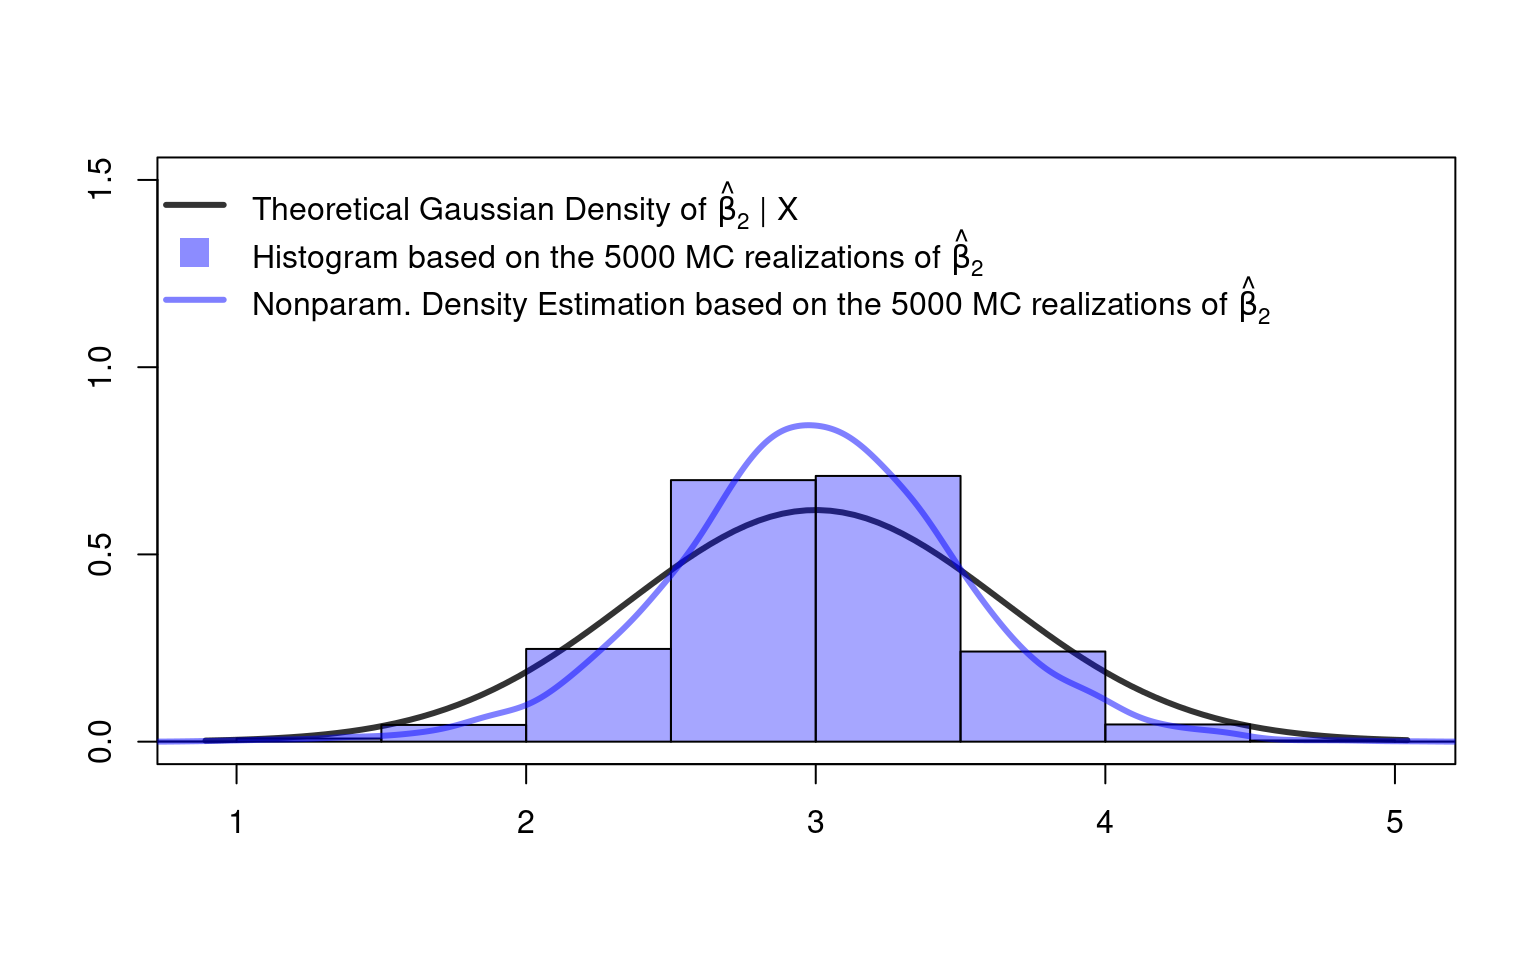
\includegraphics[width=1\textwidth]{figure/minimal-unnamed-chunk-73-1} \end{center}

Not so good. Since we do not condition on \(X\), the realizations of \(X\) affect the distribution of \(\hat\beta\) and our theoretical Gaussian distribution result in Equation \eqref{eq:ssnorm} does not apply anymore.

\hypertarget{testing-multiple-parameters}{%
\subsection{Testing Multiple Parameters}\label{testing-multiple-parameters}}

In the following, we do inference about multiple parameters. We test
\begin{align*}
H_0:&\beta_2=3\quad\text{and}\quad\beta_3=4\\
\text{versus}\quad H_A:&\beta_2\neq 3\quad\text{and/or}\quad\beta_3\neq 4.
\end{align*}
Or equivalently
\begin{align*}
H_0:&R\beta -r = 0 \\
H_A:&R\beta -r \neq 0,
\end{align*}
where
\[
R=\left(
\begin{matrix}
0&1&0\\
0&0&1\\
\end{matrix}\right)\quad\text{ and }\quad 
r=\left(\begin{matrix}3\\4\\\end{matrix}\right).
\]
The following \(\textsf{R}\) code can be used to test this hypothesis:

\begin{Shaded}
\begin{Highlighting}[]
\FunctionTok{suppressMessages}\NormalTok{(}\FunctionTok{library}\NormalTok{(}\StringTok{"car"}\NormalTok{)) }\CommentTok{\# for linearHyothesis()}
\CommentTok{\# ?linearHypothesis}

\DocumentationTok{\#\# Estimate the linear regression model parameters}
\NormalTok{lm\_obj }\OtherTok{\textless{}{-}} \FunctionTok{lm}\NormalTok{(Y }\SpecialCharTok{\textasciitilde{}}\NormalTok{ X\_2 }\SpecialCharTok{+}\NormalTok{ X\_3, }\AttributeTok{data =}\NormalTok{ mydata)}

\DocumentationTok{\#\# Option 1:}
\NormalTok{car}\SpecialCharTok{::}\FunctionTok{linearHypothesis}\NormalTok{(}\AttributeTok{model =}\NormalTok{ lm\_obj, }
                      \AttributeTok{hypothesis.matrix =} \FunctionTok{c}\NormalTok{(}\StringTok{"X\_2=3"}\NormalTok{, }\StringTok{"X\_3=4"}\NormalTok{))}
\CommentTok{\#\textgreater{} Linear hypothesis test}
\CommentTok{\#\textgreater{} }
\CommentTok{\#\textgreater{} Hypothesis:}
\CommentTok{\#\textgreater{} X\_2 = 3}
\CommentTok{\#\textgreater{} X\_3 = 4}
\CommentTok{\#\textgreater{} }
\CommentTok{\#\textgreater{} Model 1: restricted model}
\CommentTok{\#\textgreater{} Model 2: Y \textasciitilde{} X\_2 + X\_3}
\CommentTok{\#\textgreater{} }
\CommentTok{\#\textgreater{}   Res.Df    RSS Df Sum of Sq      F  Pr(\textgreater{}F)  }
\CommentTok{\#\textgreater{} 1      9 87.285                              }
\CommentTok{\#\textgreater{} 2      7 37.599  2    49.686 4.6252 0.05246 .}
\CommentTok{\#\textgreater{} {-}{-}{-}}
\CommentTok{\#\textgreater{} Signif. codes:  0 \textquotesingle{}***\textquotesingle{} 0.001 \textquotesingle{}**\textquotesingle{} 0.01 \textquotesingle{}*\textquotesingle{} 0.05 \textquotesingle{}.\textquotesingle{} 0.1 \textquotesingle{} \textquotesingle{} 1}

\DocumentationTok{\#\# Option 2:}
\NormalTok{R }\OtherTok{\textless{}{-}} \FunctionTok{rbind}\NormalTok{(}\FunctionTok{c}\NormalTok{(}\DecValTok{0}\NormalTok{,}\DecValTok{1}\NormalTok{,}\DecValTok{0}\NormalTok{),}
           \FunctionTok{c}\NormalTok{(}\DecValTok{0}\NormalTok{,}\DecValTok{0}\NormalTok{,}\DecValTok{1}\NormalTok{))}
\NormalTok{car}\SpecialCharTok{::}\FunctionTok{linearHypothesis}\NormalTok{(}\AttributeTok{model =}\NormalTok{ lm\_obj, }
                      \AttributeTok{hypothesis.matrix =}\NormalTok{ R, }
                      \AttributeTok{rhs =} \FunctionTok{c}\NormalTok{(}\DecValTok{3}\NormalTok{,}\DecValTok{4}\NormalTok{))}
\CommentTok{\#\textgreater{} Linear hypothesis test}
\CommentTok{\#\textgreater{} }
\CommentTok{\#\textgreater{} Hypothesis:}
\CommentTok{\#\textgreater{} X\_2 = 3}
\CommentTok{\#\textgreater{} X\_3 = 4}
\CommentTok{\#\textgreater{} }
\CommentTok{\#\textgreater{} Model 1: restricted model}
\CommentTok{\#\textgreater{} Model 2: Y \textasciitilde{} X\_2 + X\_3}
\CommentTok{\#\textgreater{} }
\CommentTok{\#\textgreater{}   Res.Df    RSS Df Sum of Sq      F  Pr(\textgreater{}F)  }
\CommentTok{\#\textgreater{} 1      9 87.285                              }
\CommentTok{\#\textgreater{} 2      7 37.599  2    49.686 4.6252 0.05246 .}
\CommentTok{\#\textgreater{} {-}{-}{-}}
\CommentTok{\#\textgreater{} Signif. codes:  0 \textquotesingle{}***\textquotesingle{} 0.001 \textquotesingle{}**\textquotesingle{} 0.01 \textquotesingle{}*\textquotesingle{} 0.05 \textquotesingle{}.\textquotesingle{} 0.1 \textquotesingle{} \textquotesingle{} 1}
\end{Highlighting}
\end{Shaded}

Not surprisingly, we cannot reject the null hypothesis at a significance level of, for instance, \(\alpha=0.05\) since we actually test the true null hypothesis. However, in repeated samples we should nevertheless observe \(\alpha\cdot 100\%\) type I errors (false rejections of \(H_0\)). Let's check this using the following Monte Carlo simulation:

\begin{Shaded}
\begin{Highlighting}[]
\DocumentationTok{\#\# Let\textquotesingle{}s generate 5000 F{-}test decisions and check }
\DocumentationTok{\#\# whether the empirical rate of type I errors is }
\DocumentationTok{\#\# close to the theoretical significance level. }
\NormalTok{rep             }\OtherTok{\textless{}{-}} \DecValTok{5000} \CommentTok{\# MC replications}
\NormalTok{F\_test\_pvalues  }\OtherTok{\textless{}{-}} \FunctionTok{rep}\NormalTok{(}\ConstantTok{NA}\NormalTok{, }\AttributeTok{times=}\NormalTok{rep)}
\DocumentationTok{\#\#}
\ControlFlowTok{for}\NormalTok{(r }\ControlFlowTok{in} \DecValTok{1}\SpecialCharTok{:}\NormalTok{rep)\{}
  \DocumentationTok{\#\# generate new MC\_data conditionally on X\_cond}
\NormalTok{    MC\_data }\OtherTok{\textless{}{-}} \FunctionTok{myDataGenerator}\NormalTok{(}\AttributeTok{n    =}\NormalTok{ n, }
                               \AttributeTok{beta =}\NormalTok{ beta\_true, }
                               \AttributeTok{X    =}\NormalTok{ X\_cond)}
\NormalTok{    lm\_obj            }\OtherTok{\textless{}{-}} \FunctionTok{lm}\NormalTok{(Y }\SpecialCharTok{\textasciitilde{}}\NormalTok{ X\_2 }\SpecialCharTok{+}\NormalTok{ X\_3, }\AttributeTok{data =}\NormalTok{ MC\_data)}
    \DocumentationTok{\#\# save the p{-}value}
\NormalTok{    p }\OtherTok{\textless{}{-}} \FunctionTok{linearHypothesis}\NormalTok{(lm\_obj, }
                          \FunctionTok{c}\NormalTok{(}\StringTok{"X\_2=3"}\NormalTok{, }\StringTok{"X\_3=4"}\NormalTok{))}\SpecialCharTok{$}\StringTok{\textasciigrave{}}\AttributeTok{Pr(\textgreater{}F)}\StringTok{\textasciigrave{}}\NormalTok{[}\DecValTok{2}\NormalTok{]}
\NormalTok{    F\_test\_pvalues[r] }\OtherTok{\textless{}{-}}\NormalTok{ p}
\NormalTok{\}}
\DocumentationTok{\#\#}
\NormalTok{signif\_level }\OtherTok{\textless{}{-}}  \FloatTok{0.05}
\NormalTok{rejections   }\OtherTok{\textless{}{-}}\NormalTok{ F\_test\_pvalues[F\_test\_pvalues }\SpecialCharTok{\textless{}}\NormalTok{ signif\_level]}
\FunctionTok{round}\NormalTok{(}\FunctionTok{length}\NormalTok{(rejections)}\SpecialCharTok{/}\NormalTok{rep, }\DecValTok{3}\NormalTok{)}
\CommentTok{\#\textgreater{} [1] 0.05}
\DocumentationTok{\#\# }
\NormalTok{signif\_level }\OtherTok{\textless{}{-}}  \FloatTok{0.01}
\NormalTok{rejections   }\OtherTok{\textless{}{-}}\NormalTok{ F\_test\_pvalues[F\_test\_pvalues }\SpecialCharTok{\textless{}}\NormalTok{ signif\_level]}
\FunctionTok{round}\NormalTok{(}\FunctionTok{length}\NormalTok{(rejections)}\SpecialCharTok{/}\NormalTok{rep, }\DecValTok{3}\NormalTok{)}
\CommentTok{\#\textgreater{} [1] 0.009}
\end{Highlighting}
\end{Shaded}

Note that this is actually a very strong result. First, it means that we correctly control for the type I error rate since the type I error rate is not larger than the chosen significance level \(\alpha\). Second, it means that the test is not conservative (i.e.~very efficient) since the empirical type I error rate is really close to the chosen significance level \(\alpha\). (In fact, if we would increase the number of Monte Carlo repetitions, the empirical type I error rate would converge to the selected significance level \(\alpha\) due to the law of large numbers.)

Next, we check how well the \(F\) test detects certain violations of the null hypothesis. We do this by using the same data generating process, but by testing the following incorrect null hypothesis:
\begin{align*}
H_0:&\beta_2=4\quad\text{and}\quad\beta_3=4\\
H_A:&\beta_2\neq 4\quad\text{and/or}\quad\beta_3\neq 4
\end{align*}

\begin{Shaded}
\begin{Highlighting}[]
\FunctionTok{set.seed}\NormalTok{(}\DecValTok{321}\NormalTok{)}
\NormalTok{rep             }\OtherTok{\textless{}{-}} \DecValTok{5000} \CommentTok{\# MC replications}
\NormalTok{F\_test\_pvalues  }\OtherTok{\textless{}{-}} \FunctionTok{rep}\NormalTok{(}\ConstantTok{NA}\NormalTok{, }\AttributeTok{times=}\NormalTok{rep)}
\DocumentationTok{\#\#}
\ControlFlowTok{for}\NormalTok{(r }\ControlFlowTok{in} \DecValTok{1}\SpecialCharTok{:}\NormalTok{rep)\{}
  \DocumentationTok{\#\# generate new MC\_data conditionally on X\_cond}
\NormalTok{    MC\_data }\OtherTok{\textless{}{-}} \FunctionTok{myDataGenerator}\NormalTok{(}\AttributeTok{n    =}\NormalTok{ n, }
                               \AttributeTok{beta =}\NormalTok{ beta\_true, }
                               \AttributeTok{X    =}\NormalTok{ X\_cond)}
\NormalTok{    lm\_obj            }\OtherTok{\textless{}{-}} \FunctionTok{lm}\NormalTok{(Y }\SpecialCharTok{\textasciitilde{}}\NormalTok{ X\_2 }\SpecialCharTok{+}\NormalTok{ X\_3, }\AttributeTok{data =}\NormalTok{ MC\_data)}
    \DocumentationTok{\#\# save p{-}values of all rep{-}many tests}
\NormalTok{    F\_test\_pvalues[r] }\OtherTok{\textless{}{-}} \FunctionTok{linearHypothesis}\NormalTok{(lm\_obj,}
                         \FunctionTok{c}\NormalTok{(}\StringTok{"X\_2=4"}\NormalTok{,}\StringTok{"X\_3=4"}\NormalTok{))}\SpecialCharTok{$}\StringTok{\textasciigrave{}}\AttributeTok{Pr(\textgreater{}F)}\StringTok{\textasciigrave{}}\NormalTok{[}\DecValTok{2}\NormalTok{]}
\NormalTok{\}}
\DocumentationTok{\#\#}
\NormalTok{signif\_level }\OtherTok{\textless{}{-}}  \FloatTok{0.05}
\NormalTok{rejections   }\OtherTok{\textless{}{-}}\NormalTok{ F\_test\_pvalues[F\_test\_pvalues }\SpecialCharTok{\textless{}}\NormalTok{ signif\_level]}
\FunctionTok{length}\NormalTok{(rejections)}\SpecialCharTok{/}\NormalTok{rep}
\CommentTok{\#\textgreater{} [1] 0.3924}
\end{Highlighting}
\end{Shaded}

Indeed, we can now reject the (false) null hypothesis in approximately 39\% of all resamplings from the true data generating process. \textbf{Caution:} This also means that we are not able to \say{see} the violation of the null hypothesis in \(100\%-39\%=62\%\) of cases. Therefore, we can never use an insignificant test result (p-value\(\geq\alpha\)) as a justification to accept the null hypothesis.

Moreover, note that the \(F\) test is not informative about which part of the null hypothesis (\(\beta_2=4\) and/or \(\beta_3=4\)) is violated -- we only get the information that at least one of the multiple parameter hypotheses is violated:

\begin{Shaded}
\begin{Highlighting}[]
\NormalTok{car}\SpecialCharTok{::}\FunctionTok{linearHypothesis}\NormalTok{(lm\_obj, }\FunctionTok{c}\NormalTok{(}\StringTok{"X\_2=4"}\NormalTok{, }\StringTok{"X\_3=4"}\NormalTok{))}
\CommentTok{\#\textgreater{} Linear hypothesis test}
\CommentTok{\#\textgreater{} }
\CommentTok{\#\textgreater{} Hypothesis:}
\CommentTok{\#\textgreater{} X\_2 = 4}
\CommentTok{\#\textgreater{} X\_3 = 4}
\CommentTok{\#\textgreater{} }
\CommentTok{\#\textgreater{} Model 1: restricted model}
\CommentTok{\#\textgreater{} Model 2: Y \textasciitilde{} X\_2 + X\_3}
\CommentTok{\#\textgreater{} }
\CommentTok{\#\textgreater{}   Res.Df     RSS Df Sum of Sq      F   Pr(\textgreater{}F)   }
\CommentTok{\#\textgreater{} 1      9 141.245                                }
\CommentTok{\#\textgreater{} 2      7  32.572  2    108.67 11.677 0.005889 **}
\CommentTok{\#\textgreater{} {-}{-}{-}}
\CommentTok{\#\textgreater{} Signif. codes:  0 \textquotesingle{}***\textquotesingle{} 0.001 \textquotesingle{}**\textquotesingle{} 0.01 \textquotesingle{}*\textquotesingle{} 0.05 \textquotesingle{}.\textquotesingle{} 0.1 \textquotesingle{} \textquotesingle{} 1}
\end{Highlighting}
\end{Shaded}

\hypertarget{dualty-of-confidence-intervals-and-hypothesis-tests}{%
\subsection{Dualty of Confidence Intervals and Hypothesis Tests}\label{dualty-of-confidence-intervals-and-hypothesis-tests}}

Confidence intervals can be computed using \textsf{R} as following:

\begin{Shaded}
\begin{Highlighting}[]
\NormalTok{signif\_level }\OtherTok{\textless{}{-}} \FloatTok{0.05}
\DocumentationTok{\#\# 95\% CI for beta\_2}
\FunctionTok{confint}\NormalTok{(lm\_obj, }\AttributeTok{parm =} \StringTok{"X\_2"}\NormalTok{, }\AttributeTok{level =} \DecValTok{1} \SpecialCharTok{{-}}\NormalTok{ signif\_level)}
\CommentTok{\#\textgreater{}        2.5 \%   97.5 \%}
\CommentTok{\#\textgreater{} X\_2 1.370315 3.563536}
\DocumentationTok{\#\# 95\% CI for beta\_3 }
\FunctionTok{confint}\NormalTok{(lm\_obj, }\AttributeTok{parm =} \StringTok{"X\_3"}\NormalTok{, }\AttributeTok{level =} \DecValTok{1} \SpecialCharTok{{-}}\NormalTok{ signif\_level)}
\CommentTok{\#\textgreater{}        2.5 \%   97.5 \%}
\CommentTok{\#\textgreater{} X\_3 3.195389 4.695134}
\end{Highlighting}
\end{Shaded}

We can use these two-sided confidence intervals to do hypothesis tests. For instance, when testing the null hypothesis
\begin{align*}
H_0:&\beta_3=4\\
\text{versus}\quad H_A: &\beta_3\neq 4
\end{align*}
we can check whether the confidence interval \(\operatorname{CI}_{1-\alpha}\) contains the hypothetical value \(4\) or not. In case of \(4\in \operatorname{CI}_{1-\alpha}\), we cannot reject the null hypothesis. In case of \(4\not\in \operatorname{CI}_{1-\alpha}\), we reject the null hypothesis.

If the Assumption 1-4\(^\ast\) hold true, then \(\operatorname{CI}_{1-\alpha}\) is an exact confidence interval. That is, under the null hypothesis, it falsely rejects the null hypothesis in only \(\alpha\cdot 100\%\) of resamplings. Let's check this in the following \(\textsf{R}\) code:

\begin{Shaded}
\begin{Highlighting}[]
\DocumentationTok{\#\# Let\textquotesingle{}s generate 1000 CIs }
\FunctionTok{set.seed}\NormalTok{(}\DecValTok{123}\NormalTok{)}
\NormalTok{signif\_level }\OtherTok{\textless{}{-}}  \FloatTok{0.05}
\NormalTok{rep          }\OtherTok{\textless{}{-}} \DecValTok{5000} \CommentTok{\# MC replications}
\NormalTok{confint\_m    }\OtherTok{\textless{}{-}} \FunctionTok{matrix}\NormalTok{(}\ConstantTok{NA}\NormalTok{, }\AttributeTok{nrow=}\DecValTok{2}\NormalTok{, }\AttributeTok{ncol=}\NormalTok{rep)}
\DocumentationTok{\#\#}
\ControlFlowTok{for}\NormalTok{(r }\ControlFlowTok{in} \DecValTok{1}\SpecialCharTok{:}\NormalTok{rep)\{}
  \DocumentationTok{\#\# generate new MC\_data conditionally on X\_cond}
\NormalTok{    MC\_data }\OtherTok{\textless{}{-}} \FunctionTok{myDataGenerator}\NormalTok{(}\AttributeTok{n    =}\NormalTok{ n, }
                               \AttributeTok{beta =}\NormalTok{ beta\_true, }
                               \AttributeTok{X    =}\NormalTok{ X\_cond)}
\NormalTok{    lm\_obj            }\OtherTok{\textless{}{-}} \FunctionTok{lm}\NormalTok{(Y }\SpecialCharTok{\textasciitilde{}}\NormalTok{ X\_2 }\SpecialCharTok{+}\NormalTok{ X\_3, }\AttributeTok{data =}\NormalTok{ MC\_data)}
    \DocumentationTok{\#\# save the p{-}value}
\NormalTok{    CI }\OtherTok{\textless{}{-}} \FunctionTok{confint}\NormalTok{(lm\_obj, }\AttributeTok{parm=}\StringTok{"X\_2"}\NormalTok{, }\AttributeTok{level=}\DecValTok{1}\SpecialCharTok{{-}}\NormalTok{signif\_level)}
\NormalTok{    confint\_m[,r] }\OtherTok{\textless{}{-}}\NormalTok{ CI}
\NormalTok{\}}
\DocumentationTok{\#\#}
\NormalTok{inside\_CI  }\OtherTok{\textless{}{-}}\NormalTok{ confint\_m[}\DecValTok{1}\NormalTok{,] }\SpecialCharTok{\textless{}=}\NormalTok{ beta\_true\_2 }\SpecialCharTok{\&} 
\NormalTok{                beta\_true\_2 }\SpecialCharTok{\textless{}=}\NormalTok{ confint\_m[}\DecValTok{2}\NormalTok{,]}

\DocumentationTok{\#\# CI{-}lower, CI{-}upper, beta\_true\_2 inside?}
\FunctionTok{head}\NormalTok{(}\FunctionTok{cbind}\NormalTok{(}\FunctionTok{t}\NormalTok{(confint\_m), inside\_CI))}
\CommentTok{\#\textgreater{}                         inside\_CI}
\CommentTok{\#\textgreater{} [1,] 0.8555396 3.639738         1}
\CommentTok{\#\textgreater{} [2,] 0.9143542 3.270731         1}
\CommentTok{\#\textgreater{} [3,] 1.9336526 4.984167         1}
\CommentTok{\#\textgreater{} [4,] 1.9985874 3.812695         1}
\CommentTok{\#\textgreater{} [5,] 3.0108642 5.621791         0}
\CommentTok{\#\textgreater{} [6,] 2.0967675 4.716398         1}

\FunctionTok{round}\NormalTok{(}\FunctionTok{length}\NormalTok{(inside\_CI[inside\_CI }\SpecialCharTok{==} \ConstantTok{FALSE}\NormalTok{])}\SpecialCharTok{/}\NormalTok{rep, }\DecValTok{2}\NormalTok{)}
\CommentTok{\#\textgreater{} [1] 0.05}

\NormalTok{nCIs }\OtherTok{\textless{}{-}} \DecValTok{100}
\FunctionTok{plot}\NormalTok{(}\AttributeTok{x=}\DecValTok{0}\NormalTok{,}\AttributeTok{y=}\DecValTok{0}\NormalTok{,}\AttributeTok{type=}\StringTok{"n"}\NormalTok{,}\AttributeTok{xlim=}\FunctionTok{c}\NormalTok{(}\DecValTok{0}\NormalTok{,nCIs),}\AttributeTok{ylim=}\FunctionTok{range}\NormalTok{(confint\_m[,}\DecValTok{1}\SpecialCharTok{:}\NormalTok{nCIs]),}
     \AttributeTok{ylab=}\StringTok{""}\NormalTok{, }\AttributeTok{xlab=}\StringTok{"Resamplings"}\NormalTok{, }\AttributeTok{main=}\StringTok{"Confidence Intervals"}\NormalTok{)}
\ControlFlowTok{for}\NormalTok{(r }\ControlFlowTok{in} \DecValTok{1}\SpecialCharTok{:}\NormalTok{nCIs)\{}
  \ControlFlowTok{if}\NormalTok{(inside\_CI[r]}\SpecialCharTok{==}\ConstantTok{TRUE}\NormalTok{)\{}
      \FunctionTok{lines}\NormalTok{(}\AttributeTok{x=}\FunctionTok{c}\NormalTok{(r,r), }\AttributeTok{y=}\FunctionTok{c}\NormalTok{(confint\_m[}\DecValTok{1}\NormalTok{,r], confint\_m[}\DecValTok{2}\NormalTok{,r]), }
            \AttributeTok{lwd=}\DecValTok{2}\NormalTok{, }\AttributeTok{col=}\FunctionTok{gray}\NormalTok{(.}\DecValTok{5}\NormalTok{,.}\DecValTok{5}\NormalTok{))}
\NormalTok{  \}}\ControlFlowTok{else}\NormalTok{\{}
      \FunctionTok{lines}\NormalTok{(}\AttributeTok{x=}\FunctionTok{c}\NormalTok{(r,r), }\AttributeTok{y=}\FunctionTok{c}\NormalTok{(confint\_m[}\DecValTok{1}\NormalTok{,r], confint\_m[}\DecValTok{2}\NormalTok{,r]), }
            \AttributeTok{lwd=}\DecValTok{2}\NormalTok{, }\AttributeTok{col=}\StringTok{"darkred"}\NormalTok{)}
\NormalTok{    \}}
\NormalTok{\}}
\FunctionTok{axis}\NormalTok{(}\DecValTok{4}\NormalTok{, }\AttributeTok{at=}\NormalTok{beta\_true\_2, }\AttributeTok{labels =} \FunctionTok{expression}\NormalTok{(beta[}\DecValTok{2}\NormalTok{]))}
\FunctionTok{abline}\NormalTok{(}\AttributeTok{h=}\NormalTok{beta\_true\_2)}
\end{Highlighting}
\end{Shaded}

\begin{center}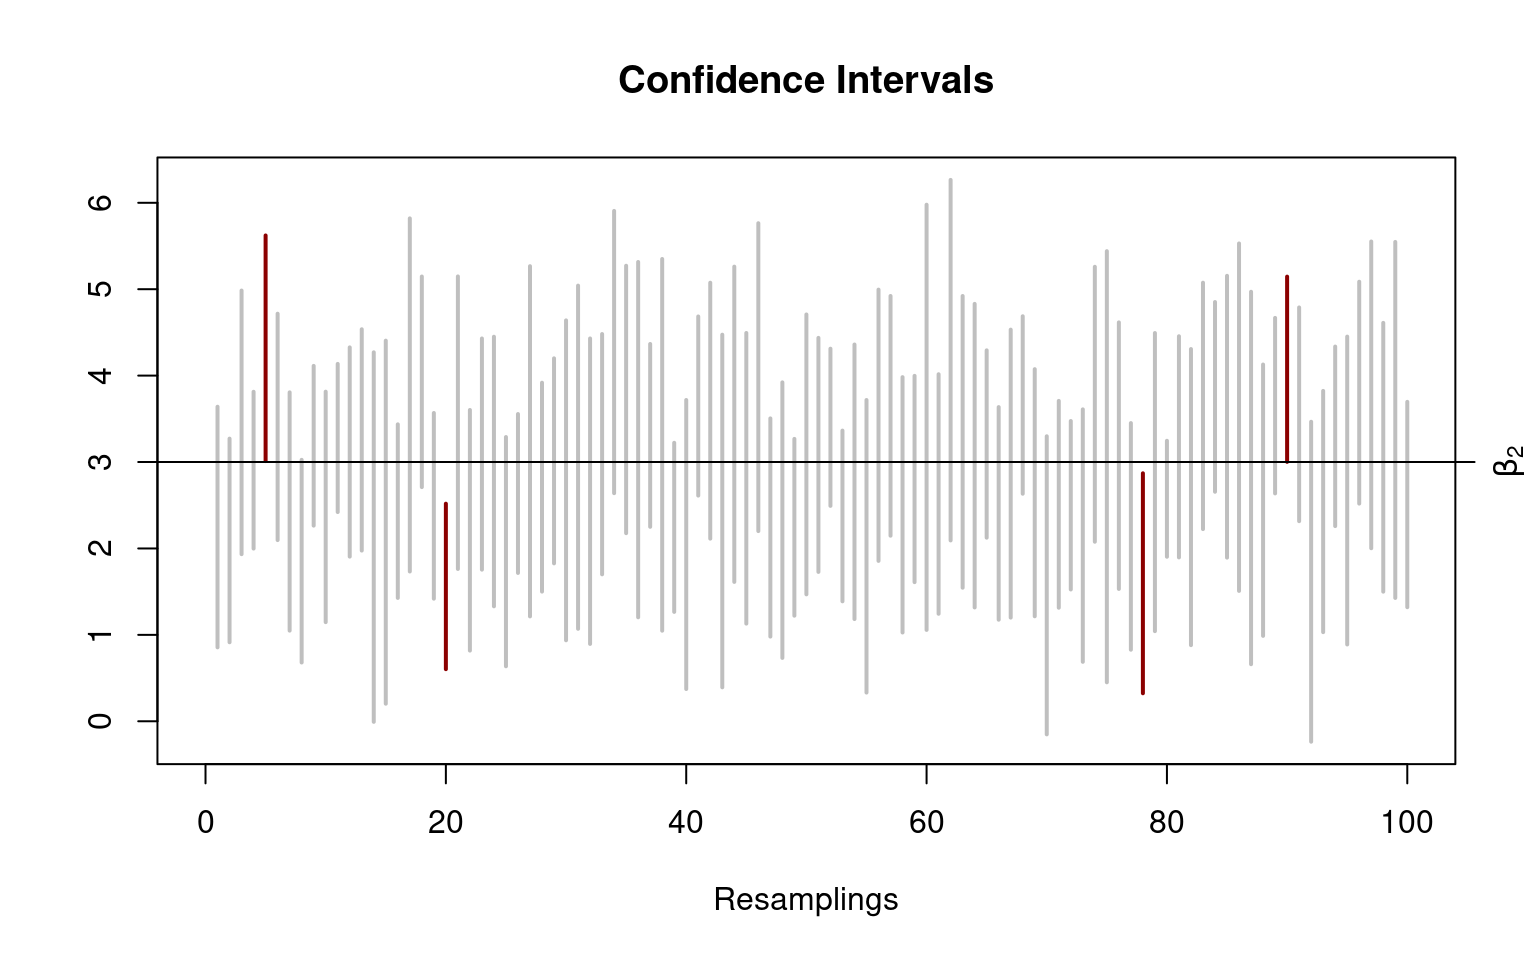
\includegraphics[width=1\textwidth]{figure/minimal-unnamed-chunk-79-1} \end{center}

\hypertarget{ch:LSINF}{%
\chapter{Large Sample Inference}\label{ch:LSINF}}

\hypertarget{tools-for-asymptotic-statistics}{%
\section{Tools for Asymptotic Statistics}\label{tools-for-asymptotic-statistics}}

\hypertarget{modes-of-convergence}{%
\subsection{Modes of Convergence}\label{modes-of-convergence}}

In the following we will discuss the four most important convergence concepts for sequences of random variables \((z_1,z_2,\dots,z_n)\) shortly denoted by \(\{z_n\}\). Non-random scalars (or vectors or matrices) will be denoted by Greek letters such as \(\alpha\).

\hypertarget{four-important-modes-of-convergence}{%
\subsection*{Four Important Modes of Convergence}\label{four-important-modes-of-convergence}}
\addcontentsline{toc}{subsection}{Four Important Modes of Convergence}

\paragraph*{1.~Convergence in Probability:}

A sequence of random scalars \(\{z_n\}\) \textbf{converges in probability} to a constant (non-random) \(\alpha\) if, for any (arbitrarily small) \(\eps>0\),
\begin{eqnarray*}
  \lim_{n\to\infty} P\left(|z_n-\alpha|>\eps\right)=0.
\end{eqnarray*}
We write: \(\plim_{n\to\infty}z_n=\alpha\), or \(z_n\toprob\alpha\). Convergence in probability of a sequence of random vectors (or matrices) \(\{z_n\}\) to a constant vector (or matrix) \(\alpha\) requires \emph{element-wise} convergence in probability.

\paragraph*{2.~Almost Sure Convergence:}

A sequence of random scalars \(\{z_n\}\) \textbf{converges almost surely} to a constant (non-random) \(\alpha\) if
\begin{eqnarray*}
P\left(\lim_{n\to\infty}z_n=\alpha\right)=1.
\end{eqnarray*}
We write: \(z_n\toas\alpha\). Almost sure convergence of a sequence of random vectors (or matrices) \(\{z_n\}\) to a constant vector (or matrix) \(\alpha\) requires \emph{element-wise} almost sure convergence.

\paragraph*{Note.}

Almost sure convergence is (usually) rather hard to derive, since the probability is about an event concerning an infinite sequence. Fortunately, however, there are established strong laws of large numbers that we can use for showing almost sure convergence.

\paragraph*{3.~Convergence in Mean Square:}

A sequence of random scalars \(\{z_n\}\) \textbf{converges in mean square} (or \textbf{in quadratic mean}) to a constant (non-random) \(\alpha\) if
\begin{eqnarray*}
  \lim_{n\to\infty}E\left((z_n-\alpha)^2\right)=0
\end{eqnarray*}
We write: \(z_n\toms\alpha\). If \(z_n\) is an estimator (e.g., \(z_n=\hat\beta_{k,n}\)) the expression \(E\left((z_n-\alpha)^2\right)\) is termed the \textbf{mean squared error}: \(\text{MSE}(z_n)=E\left((z_n-\alpha)^2\right)\). Mean square convergence of a sequence of random vectors (or matrices) \(\{z_n\}\) to a deterministic vector (or matrix) \(\alpha\) requires \emph{element-wise} mean square convergence.

\paragraph*{4.~Convergence in Distribution:}

Let \(F_n\) be the cumulative distribution function (cdf) of \(z_n\) and \(F\) the cdf of \(z\). A sequence of random scalars \(\{z_n\}\) \textbf{converges in distribution} to a random scalar \(z\) if for all \(t\) such that \(F(t)\) is continuous at \(t\),
\begin{eqnarray*}
  \lim_{n\to\infty}F_n(t)=F(t).
\end{eqnarray*}
We write: \(z_n\todistr z\) and call \(F\) the \textbf{asymptotic} (or \textbf{limit}) \textbf{distribution} of \(z_n\). Sometimes you will see statements like \(z_n\todistr N(0,1)\) or \(z_n\overset{a}{\sim}N(0,1)\), which should be read as \(z_n\todistr z\), where \(z\sim N(0,1)\).

\paragraph*{Note.}

A stochastic sequence \(\{z_n\}\) can also convergence in distribution to a \textbf{deterministic scalar} \(\alpha\). In this case \(\alpha\) is treated as a degenerated random variable with cdf
\[
F_\alpha(t)=\left\{\begin{matrix}0&\text{if}\;\;t<\alpha\\ 1&\text{if}\;\;t\geq\alpha\end{matrix}\right.
\]

\paragraph*{4$^\prime$. Multivariate Convergence in Distribution:}

Let \(z_n,z\in\mathbb{R}^K\) be \(K\)-dimensional random variables, then
\[
z_n\todistr z\text{\quad if and only if \quad}\lambda'z_n\todistr\lambda'z
\]
for any \(\lambda\in\mathbb{R}^K\). This statement is known as the \textbf{Cram\'er Wold Device}. It is needed since element-wise convergence in distribution does generally not imply convergence of the \emph{joint} distribution of \(z_n\) to the \emph{joint} distribution of \(z\); except, if all elements are independent from each other.

\hypertarget{relations-among-modes-of-convergence}{%
\subsection*{Relations among Modes of Convergence}\label{relations-among-modes-of-convergence}}
\addcontentsline{toc}{subsection}{Relations among Modes of Convergence}

\begin{lemma}\label{Relations}\textbf{\textrm{Relationship among the four modes of convergence:}}
\begin{itemize}
\item[(i)] $z_n\toms\alpha\Rightarrow z_n\toprob\alpha.$
\item[(ii)] $z_n\toas\alpha\Rightarrow z_n\toprob\alpha.$ 
\item[(iii)] $z_n\todistr\alpha\Leftrightarrow z_n\toprob\alpha.$ I.e., if the limiting random variable is a constant (i.e., a degenerated random variable), then convergence in distribution is equivalent to convergence in probability.
\end{itemize}
\end{lemma}

\noindent Proofs can be found, e.g., here: \url{https://www.statlect.com/asymptotic-theory/relations-among-modes-of-convergence}

\hypertarget{continuous-mapping-theorem-cmt}{%
\subsection{Continuous Mapping Theorem (CMT)}\label{continuous-mapping-theorem-cmt}}

\begin{lemma}\label{Preserv}\textbf{Preservation of convergence for continuous transformations (or "continuous mapping theorem (CMT)"):} Suppose $\{z_n\}$ is a stochastic sequence of random scalars, vectors, or matrices and that $a(\cdot)$ is a continuous function that does not depended on $n$. Then
\begin{itemize}
\item[(i)] $z_n\toprob\alpha\Rightarrow a(z_n)\toprob a(\alpha)$
\item[(ii)]$z_n\toas  \alpha\Rightarrow a(z_n)\toas a(\alpha)$
\item[(iii)]$z_n\todistr\alpha\Rightarrow a(z_n)\todistr a(\alpha)$
\end{itemize}
\end{lemma}

\noindent Proof can be found, e.g., in \emph{Asymptotic Statistics}, van der Vaart (1998), Theorem 2.3. Or here: \url{https://www.statlect.com/asymptotic-theory/continuous-mapping-theorem}

\paragraph*{Note.}

The CMT does \emph{not} hold for m.s.-convergence except for the case where \(a(.)\) is linear.\\

\paragraph*{Examples.}

As a consequence of the CMT (Lemma \ref{Preserv}) we have that the usual arithmetic operations preserve convergence in probability (equivalently for almost sure convergence and convergence in distribution):

\begin{itemize}
\item[] If $x_n\toprob \beta$\quad and \quad $y_n\toprob \gamma$ \quad then\;\; $x_n+y_n\toprob \beta+\gamma$
\item[] If $x_n\toprob \beta$\quad and \quad $y_n\toprob \gamma$ \quad then\;\; $x_n\cdot y_n\toprob \beta\cdot\gamma$
\item[] If $x_n\toprob \beta$\quad and \quad $y_n\toprob \gamma$ \quad then\; $x_n/y_n\toprob \beta/\gamma$, \quad provided that $\gamma\neq 0$
\item[] If $X_n'X_n\toprob \Sigma_{X'X}$ \quad then\; $(X_n'X_n)^{-1}\toprob \Sigma_{X'X}^{-1}$, provided $\Sigma_{X'X}$ is a nonsingular matrix.
\end{itemize}

\hypertarget{slutsky-theorem}{%
\subsection{Slutsky Theorem}\label{slutsky-theorem}}

The following results are concerned with combinations of convergence in probability and convergence in distribution. These are particularly important for the derivation of the asymptotic distribution of estimators.\\

\begin{lemma}[Slutsky Theorem]\label{Slutsky} Let $x_n$ and $y_n$ denote sequences of random scalars or vectors and let $A_n$ denote a sequences of random matrices. Moreover, $\alpha$ and $A$ are deterministic limits of appropriate dimensions and $x$ is a random limit of appropriate dimension. 
\begin{itemize}
  \item[(i)] If $x_n\todistr x$\quad and \quad $y_n\toprob \alpha$ \quad then\;\; $x_n+y_n\todistr x+\alpha$
  \item[(ii)] If $x_n\todistr x$\quad and \quad $y_n\toprob 0$ \quad then\;\; $x_n'y_n\toprob 0$
  \item[(iii)] If $x_n\todistr x$\quad and \quad $A_n\toprob A$ \quad then\;\; $A_nx_n\todistr Ax$, where it is assumed that $A_n$ and $x_n$ are \say{conformable} (i.e., the matrix- and vector-dimensions fit to each other). \\[2ex]
Important special case:\\
If $x_n\todistr N(0,\Sigma)$\quad and \quad $A_n\toprob A$ \quad then\;\; $A_nx_n\todistr N(0,A\Sigma A')$
\end{itemize}  
\end{lemma}

\noindent Proofs can be found, e.g., in \emph{Asymptotic Statistics}, van der Vaart, Theorem 2.8. Or here: \url{https://www.statlect.com/asymptotic-theory/Slutsky-theorem}

\paragraph*{Note.}

Sometimes, only parts \textit{(i)} and \textit{(ii)} of Lemma \ref{Slutsky} are called \say{Slutsky's theorem.}

\hypertarget{law-of-large-numbers-lln-and-central-limit-theorem-clt}{%
\subsection{Law of Large Numbers (LLN) and Central Limit Theorem (CLT)}\label{law-of-large-numbers-lln-and-central-limit-theorem-clt}}

So far, we discussed the definitions of the four most important convergence modes, their relations among each other, and basic theorems (CMT and Slutsky) about functionals of stochastic sequences. Though, we still lack of tools that allow us to actually show that a stochastic sequence convergences (in some of the discussed modes) to some limit.

In the following we consider the stochastic sequences \(\{\bar{z}_n\}\) of sample means \(\bar{z}_n=n^{-1}\sum_{i=1}^nz_i\), where \(z_i\), \(i=1,\dots,n\), are (scalar, vector, or matrix-valued) \emph{random variables}. Remember: the sample mean \(\bar{z}_n\) is an estimator of the deterministic population mean \(\mu\).

Weak LLNs, strong LLNs, and CLTs tell us conditions under which arithmetic means \(\bar{z}_n=n^{-1}\sum_{i=1}^nz_i\) converge:
\begin{eqnarray*}
  \bar{z}_n&\toprob&\mu\quad\text{(weak LLN)}\\
  \bar{z}_n&\toas&\mu\quad\text{(strong LLN)}\\
  \sqrt{n}(\bar{z}_n-\mu)&\todistr&N(0,\sigma^2)\quad\text{(CLT)}
\end{eqnarray*}

In the following we introduce the most well-known versions of the weak, the strong LLN, and the CLT.

\bigskip

\begin{theorem}[Weak LLN (Chebychev)]\label{WLLN1}
$$\textit{If}\quad\lim_{n\to\infty} E(\bar{z}_n)=\mu\quad\textit{and}\quad\lim_{n\to\infty}\V(\bar{z}_n)=0\quad\textit{then}\quad\bar{z}_n\toprob\mu$$
\end{theorem}

\noindent Proof can be found, for instance, here: \url{https://www.statlect.com/asymptotic-theory/law-of-large-numbers}

\bigskip

\begin{theorem}[Strong LLN (Kolmogorov)]\label{SLLN1}
$$\textit{If}\;\{z_i\}\;\text{is an iid~sequence}\quad\textit{and}\quad E(z_i)=\mu\quad\textit{then}\quad\bar{z}_n\toas\mu$$
\end{theorem}

\noindent Proof can be found, e.g., in \textit{Linear Statistical Inference and Its Applications}, Rao (1973), pp.~112-114.

\paragraph*{Note.}

The weak and the strong LLN for random vectors follow from requiring element-by-element convergence.

\begin{theorem}[CLT (Lindeberg-Levy)]\label{CLT1}
$$\text{If}\;\{z_i\}\;\text{is an iid sequence}\quad\text{and}\quad E(z_i)=\mu\quad\textit{and}\quad\V(z_i)=\sigma^2\;\;\textit{then}$$
$$\sqrt{n}(\bar{z}_n-\mu)\todistr N(0,\sigma^2)\quad\text{as}\quad n\to\infty$$
\end{theorem}

\noindent Proof can be found, e.g., in \emph{Asymptotic Statistics}, van der Vaart (1998), Theorem 2.17.

\bigskip

The Lindeberg-Levy CLT for \(K\)-dimensional random vectors follows from our above discussion on \say{Multivariate Convergence in Distribution.} From this we know that if \(\bar{z}_n\in\mathbb{R}^K\) and \(\mu\in\mathbb{R}^K\), then
\[\sqrt{n}(\bar{z}_n-\mu)\todistr \mathcal{N}(0,\Sigma)\quad\Leftrightarrow\quad \sqrt{n}(\lambda'\bar{z}_n-\lambda'\mu)\todistr \mathcal{N}(0,\lambda'\Sigma\lambda),\]
for any \(\lambda\in\mathbb{R}^K\).

That is, to apply the Lindeberg-Levy CLT (Theorem \ref{CLT1}) to multivariate (e.g., \(K\)-dimensional) stochastic sequences, we need to check whether the univariate stochastic sequence \(\{\lambda'z_i\}\) is i.i.d. with \(E(\lambda'z_i)=\lambda'\mu\) and \(\V(\lambda'z_i)=\lambda'\Sigma\lambda\) for any \(\lambda\in\mathbb{R}^K\). This is the case if the multivariate (\(K\)-dimensional) stochastic sequence \(\{z_i\}\) is an i.i.d. sequence with \(E(z_i)=\mu\) and \(\V(z_i)=\Sigma\).

\paragraph*{Note.}

The LLNs and the CLT are stated with respect to sequences of sample means \(\{\bar{z}_n\}\); i.e., the simplest estimators you probably can think of. We will see, however, that this is all we need in order to analyze also more complicated estimators such as the OLS estimator.

\hypertarget{estimators-as-a-sequences-of-random-variables}{%
\subsection{Estimators as a Sequences of Random Variables}\label{estimators-as-a-sequences-of-random-variables}}

Our concepts above readily apply to general scalar-valued (univariate) or vector-valued (\(K\)-dimensional) estimators, say \(\hat\theta_n\in\mathbb{R}^K\), that are computed from i.i.d. random samples.

\paragraph*{(Weak) Consistency:}

We say that an estimator \(\hat\theta_n\) is \emph{(weakly) consistent for $\theta$} if
\[\hat\theta_n\toprob\theta\quad\text{as}\quad n\to\infty\]

\paragraph*{Asymptotic Bias:}

The \emph{asymptotic bias} of an estimator \(\hat\theta_n\) of some true parameter \(\theta\) is defined as:
\[\text{ABias}(\hat\theta_n)=\lim_{n\to\infty}E(\hat\theta_n)-\theta\]
If \(\text{ABias}(\hat\theta_n)=0\), then \(\hat\theta\) is called an \textbf{asymptotically unbiased}.

\paragraph*{Asymptotic Normality:}

A consistent estimator \(\hat\theta_n\) is \emph{asymptotically normal distributed} if
\[\sqrt{n}(\hat\theta_n-\theta)\todistr \mathcal{N}(0,\Sigma)\quad\text{as}\quad n\to\infty\]
where \(\lim_{n\to\infty}\V(\sqrt{n}(\hat\theta_n-\theta))=\lim_{n\to\infty}\V(\sqrt{n}\hat\theta_n)=\Sigma\) as called the asymptotic variance of \(\sqrt{n}(\hat\theta_n-\theta)\).

\paragraph*{$\sqrt{n}$-consistent:}

Consistent estimators \(\hat{\theta}_n\toprob\theta\) are called \emph{$\sqrt{n}$-consistent} if
\[\sqrt{n}(\hat\theta_n-\theta)\todistr z \quad\text{as}\quad n\to\infty\]
If additionally the random vector \(z\) is normal distributed, then \(\hat\theta_n\) is often called \emph{consistent and asymptotically normal.}

\hypertarget{asymptotics-under-the-classic-regression-model}{%
\section{Asymptotics under the Classic Regression Model}\label{asymptotics-under-the-classic-regression-model}}

Given the above introduced machinery on asymptotic concepts and results, we can now proof that the OLS estimators \(\hat\beta\) and \(s_{UB}^2\) applied to the classic regression model (defined by Assumptions 1-4 in Chapter \ref{ch:MLR}) are consistent and asymptotically normal distributed estimators as \(n\to\infty\). That is, we can drop the unrealistic normality and spherical errors assumption (Assumption 4\(^\ast\)), but still use the usual test statistics (t-test, F-test); as long as the sample size \(n\) is \say{large.}

However, before we can formally state the asymptotic properties, we first need to adjust our \say{data generating process} assumption (Assumption 1) such that we can apply Kolmogorov's strong LLN and Lindeberg-Levy's CLT. Second, we need to adjust the rank assumption (Assumption 3), such that the full column rank of \(X\) is guaranteed for the limiting case as \(n\to\infty\), too. Assumptions 2 and 4 from Chapter \ref{ch:MLR} are assumed to hold.

\paragraph*{Assumption 1$^\ast$: Data Generating Process (for Asymptotics)}

Assumption 1 of Chapter \ref{ch:MLR} applies, but \emph{additionally} we assume that \((\eps_i, X_i)\in\mathbb{R}^{K+1}\) (or equivalently \((Y_i,X_i)\in\mathbb{R}^{K+1}\)) is jointly i.i.d. for all \(i=1,\dots,n\), with existing and finite second moments for \(X_i\) and fourth moments for \(\eps_i\).

\paragraph*{Note 1.}

The fourth moment of \(\eps_i\) is actually only needed for Theorem \ref{Consistency_s1}; for the rest two moments are sufficient.

\paragraph*{Note 2.}

The above adjustment of Assumption 1 is far less restrictive than assuming that the error-terms \(\eps_i\) are i.i.d. normally distributed and independent from \(X_i\) (as it's necessary for small sample inference in Chapter \ref{ch:SSINF}).

\paragraph*{Assumption 3$^\ast$: Rank Condition (for Asymptotics)}

The \((K\times K)\) limiting matrix
\[\Sigma_{X'X}:=E(S_{X'X})=E(n^{-1}X'X)=E(X_iX_i')\]
has full rank \(K\). I.e., \(\Sigma_{X'X}\) is nonsingular and invertible.

\bigskip

\begin{theorem}[Consistency of $S_{X'X}^{-1}$]\label{Sxx1} Under Assumption 1$^\ast$ and 3$^\ast$ we have that
$$\left(\frac{1}{n}\X'\X\right)^{-1}=S_{X'X}^{-1}\quad\toprob\quad\Sigma_{X'X}^{-1}\quad\text{as}\quad n\to\infty$$
\end{theorem}

\noindent Proof is done in the lecture.

\begin{theorem}[Consistency of $\hat\beta$]\label{bconsistent1} Under Assumption 1$^\ast$, 2 and 3$^\ast$ we have that
$$\hat\beta_n\toprob\beta\quad\text{as}\quad n\to\infty$$
\end{theorem}

\noindent Proof is done in the lecture.

Furthermore, we can show that the appropriately scaled (by \(\sqrt{n}\)) sampling error \(\hat\beta-\beta\) of the OLS estimator is asymptotically normal distributed.

\begin{theorem}[Sampling error limiting normality (the classic case)]\label{OLSnormality1} 
For simplicity, we consider here the special case of spherical error ($\V(\eps|X)=\sigma^2I_n$). Under Assumption 1$^\ast$, 2 and 3$^\ast$ we then have that
$$\sqrt{n}(\hat\beta_n-\beta)\todistr \mathcal{N}\left(0,\sigma^2 \Sigma^{-1}_{X'X}\right)\quad\text{as}\quad n\to\infty$$
\end{theorem}

\noindent Proof is done in the lecture.

In principle, we can derive the usual test statistics from the latter result. Though, as long as we do not know (we usually don't) \(\sigma^2\) and \(\Sigma_{X'X}\) we need to plug-in the (consistent!) estimators \(S_{X'X}^{-1}\) and \(s_{UB}^2\), where the consistency of the former estimator is provided by Theorem \ref{Sxx1} and the consistency of \(s_{UB}^2\) is provided by the following result.

\begin{theorem}[Consistency of $s^2_{UB}$]\label{Consistency_s1}
$$s_{UB}^2\toprob\sigma^2\quad\text{as}\quad n\to\infty$$
\end{theorem}

\noindent Proof is skipped, but a detailed proof can be found here: \url{https://www.statlect.com/fundamentals-of-statistics/OLS-estimator-properties}

\hypertarget{the-case-of-heteroscedasticity}{%
\subsection{The Case of Heteroscedasticity}\label{the-case-of-heteroscedasticity}}

Theorem \ref{OLSnormality1} can also be stated and proofed for conditionally heteroscedastic error terms. In this case one gets
\begin{align}\label{OLSnormality1Rob}
\sqrt{n}(\hat\beta_n-\beta)\todistr \mathcal{N}\left(0,\Sigma_{X'X}^{-1}E(\eps^2_iX_iX_i')\Sigma_{X'X}^{-1}\right)\quad\text{as}\quad n\to\infty
\end{align}
where \(\Sigma_{X'X}^{-1}E(\eps_i^2X_iX_i')\Sigma_{X'X}^{-1}\) (i.e., the asymptotic variance of \(\sqrt{n}(\hat\beta_n-\beta)\)) is usually unknown and needs to be estimated from the data by
\[
S_{X'X}^{-1}\widehat{E}(\eps^2_iX_iX_i')S^{-1}_{X'X}\toprob \Sigma_{X'X}^{-1}E(\eps^2_iX_iX_i')\Sigma_{X'X}^{-1}\quad\text{as}\quad n\to\infty,
\]
where \(\widehat{E}(\eps^2_iX_iX_i')\) denotes some consistent estimator of \(E(\eps^2X_iX_i')\) such as one of the followingt choices:
\begin{align*}
\hspace*{-2cm}\text{HC0:}\quad & \widehat{E}(\eps^2_iX_iX_i')=\frac{1}{n}\sum_{i=1}^n\hat\eps_i^2X_iX_i'\\
\text{HC1:}\quad & \widehat{E}(\eps^2_iX_iX_i')=\frac{1}{n}\sum_{i=1}^n\frac{n}{n-K}\hat\eps_i^2X_iX_i'\\
\text{HC2:}\quad & \widehat{E}(\eps^2_iX_iX_i')=\frac{1}{n}\sum_{i=1}^n\frac{\hat{\eps}_{i}^{2}}{1-h_{i}}X_iX_i'\\
\text{HC3:}\quad & \widehat{E}(\eps^2_iX_iX_i')=\frac{1}{n}\sum_{i=1}^n\frac{\hat{\eps}_{i}^{2}}{\left(1-h_{i}\right)^{2}}X_iX_i'\text{\quad($\leftarrow$ Most often used)}\\
\text{HC4:}\quad & \widehat{E}(\eps^2_iX_iX_i')=\frac{1}{n}\sum_{i=1}^n\frac{\hat{\eps}_{i}^{2}}{\left(1-h_{i}\right)^{\delta_{i}}}X_iX_i'
\end{align*}
(These are the heteroscedasticity-consistent robust estimators from Chapter \ref{ch:VarEstBeta}.

\paragraph*{Note.}

In order to show that any of the above versions (HC0-4) of \(\widehat{E}(\eps^2_iX_iX_i')\) is a consistent estimator of \(E(\eps^2_iX_iX_i')\) we actually need to assume that the explanatory variables in \(X\) have finite \emph{fourth} moments \cite[see][Chapter 2.5]{Hayashi2000}. So, for this, we would need to make our Assumption 1\(^\ast\) more restrictive (so far, only two moments are assumed for \(X\)).

\hypertarget{hypothesis-testing-and-confidence-intervals}{%
\subsection{Hypothesis Testing and Confidence Intervals}\label{hypothesis-testing-and-confidence-intervals}}

From our asymptotic results under the classic regression model (Assumptions 1\(^\ast\), 2, 3\(^\ast\), and 4) we get the following results important for testing statistical hypothesis.

\hypertarget{robust-hypothesis-testing-multiple-parameters}{%
\subsubsection{Robust Hypothesis Testing: Multiple Parameters}\label{robust-hypothesis-testing-multiple-parameters}}

Let us reconsider the following system of \(q\)-many null hypotheses:
\begin{align*}
H_0: \underset{(q\times K)}{R}\underset{(K\times 1)}{\beta} - \underset{(q\times 1)}{r} = \underset{(q\times 1)}{0},
\end{align*}
where the \((q \times K)\) matrix \(R\) and the \(q\)-vector \(r=(r_{1},\dots,r_{q})'\) are chosen by the statistician to specify her/his null hypothesis about the unknown true parameter vector \(\beta\). To make sure that there are no redundant equations, it is required that \(\rank(R)=q\).

By contrast to the multiple parameter tests for small samples (see Chapter \ref{ch:testmultp}), we can work here with a heterosedasticity robust test statistic which is applicable for heteroscedastic error terms:
\begin{equation}\label{Ftestasymp}
W=n(R\hat\beta_n -r)'[R\,S_{X'X}^{-1}\widehat{E}(\eps^2_iX_iX_i')S^{-1}_{X'X}\,R']^{-1}(R\hat\beta_n-r)\overset{H_0}{\to}_d\chi^2(q)
\end{equation}
as \(n\to\infty\). The price to pay is that the distribution of the test statistic under the null hypothesis is only valid asymptotically for large \(n\). That is, the critical values taken from the asymptotic distribution will be useful only for \say{large} samples sizes. In case of homoscedastic error terms, one can substitute \(S_{X'X}^{-1}\widehat{E}(\eps^2_iX_iX_i')S^{-1}_{X'X}\) by \(s_{UB}^2S_{X'X}^{-1}\).

\paragraph*{Finite-sample correction.}

In order to improve the finite-sample performance of this test, one usually uses the \(F_{q,n-K}\) distribution with \(q\) and \(n-K\) degrees of freedoms instead of the \(\chi^2(q)\) distribution. Asymptotically (\(n\to\infty\)), \(F_{q,n-K}\) is equivalent to \(\chi^2(q)\). However, for finite sample sizes \(n\) (i.e., the practically relevant case) \(F_{q,n-K}\) leads to larger critical values which helps to account for the estimation errors in \(S_{X'X}^{-1}\widehat{E}(\eps^2_iX_iX_i')S^{-1}_{X'X}\) (or in \(s_{UB}^2S_{X'X}^{-1}\)) which are otherwise neglected by the pure asymptotic perspective.

\hypertarget{robust-hypothesis-testing-single-parameters}{%
\subsubsection{Robust Hypothesis Testing: Single Parameters}\label{robust-hypothesis-testing-single-parameters}}

Let us reconsider the case of hypotheses about only one parameter \(\beta_k\), with \(k=1,\dots,K\)
\begin{equation*}
\begin{array}{ll}
H_0: & \beta_k=r\\
H_A: & \beta_k\ne r\\
\end{array}
\end{equation*}
We can selecting the \(k\)th diagonal element of the test-statistic in \eqref{Ftestasymp} and taking the square root yields
\[
t=\frac{\sqrt{n}\left(\hat{\beta}_k-r\right)}{\sqrt{\left[S_{X'X}^{-1}\widehat{E}(\eps^2_iX_iX_i')S^{-1}_{X'X}\right]_{kk}}}\overset{H_0}{\to}_d\mathcal{N}(0,1).
\]
This \(t\) test statistic allows for heteroscedastic error terms. In case of homoscedastic error terms, one can substitute \([S_{X'X}^{-1}\widehat{E}(\eps^2_iX_iX_i')S^{-1}_{X'X}]_{kk}\) by \(s_{UB}^2[S_{X'X}^{-1}]_{kk}\).

\paragraph*{Finite-sample correction.}

In order to improve the finite-sample performance of this \(t\) test, one usually uses the \(t_{(n-K)}\) distribution with \(n-K\) degrees of freedoms instead of the \(\mathcal{N}(0,1)\) distribution. Asymptotically (\(n\to\infty\)), \(t_{(n-K)}\) is equivalent to \(\mathcal{N}(0,1)\). However, for finite sample sizes \(n\) (i.e., the practically relevant case) \(t_{n-K}\) leads to larger critical values which helps to account for the estimation errors in \([S_{X'X}^{-1}\widehat{E}(\eps^2_iX_iX_i')S^{-1}_{X'X}]_{kk}\) (or in \(s_{UB}^2[S_{X'X}^{-1}]_{kk}\)) which are otherwise neglected by the pure asymptotic perspective.

\hypertarget{robust-confidence-intervals}{%
\subsubsection{Robust Confidence Intervals}\label{robust-confidence-intervals}}

Following the derivations in Chapter \ref{CIsmallsample}, but using the expression for the robust standard errors, we get the following heteroscedasticity robust (random) \((1-\alpha)\cdot 100\%\) confidence interval
\[
\operatorname{CI}_{1-\alpha}=
\left[\hat\beta_k\pm t_{1-\alpha/2,n-K}\sqrt{n^{-1}[S_{X'X}^{-1}\widehat{E}(\eps^2_iX_iX_i')S^{-1}_{X'X}]_{kk}}\right].
\]
Here, the coverage probability is an asymptotic coverage probability with \(P(\beta_k\in\operatorname{CI}_{1-\alpha})\to 1-\alpha\) as \(n\to\infty\).

\hypertarget{practice-large-sample-inference}{%
\section{Practice: Large Sample Inference}\label{practice-large-sample-inference}}

Let's apply the above asymptotic inference methods using \textsf{R}. As in Chapter \ref{PSSI} we, first, program a function \texttt{myDataGenerator()} which allows us to generate data from the following model, i.e., from the following fully specified data generating process:
\begin{align*}
Y_i &=\beta_1+\beta_2X_{i2}+\beta_3X_{i3}+\eps_i,\qquad i=1,\dots,n\\
\beta &=(\beta_1,\beta_2,\beta_3)'=(2,3,4)'\\
X_{i2}&\sim U[-4,4]\\
X_{i3}&\sim U[-5,5]\\
\eps_i|X_i&\sim U[-0.5 |X_{i2}|, 0.5 |X_{i2}|],
\end{align*}
where \((Y_i,X_i)\) is assumed i.i.d. across \(i=1,\dots,n\) with \(X_{i2}\) and \(X_{i3}\) being independent of each other. Note that, by contrast to Chapter \ref{PSSI}, the error terms are conditionally heteroscedastic (\(\V(\eps_i|X_i)=\frac{1}{12}X_{i2}^2\)) and not Gaussian.

As a side note: The unconditional variance follows by the law of total variance and is given by \(\V(\eps_i)=E(\V(\eps_i|X_i))+\V(E(\eps_i|X_i))=E(\frac{1}{12}X_{i2}^2)+0=\frac{1}{(12)}(\frac{1}{(12)}(4-(-4))^2)=\frac{4}{9}\)).

Moreover, by contrast to Chapter \ref{PSSI}, we here do not need to sample new realizations of \(Y_1,\dots,Y_n\) conditionally on a given data matrix \(X\) since the asymptotic normality statement is not conditionally on \(X\). (The small sample normality result in \eqref{eq:ssnorm} in Chapter \ref{PSSI} is conditionally on \(X\); however, the large sample normality result in (\ref{OLSnormality1Rob}) is unconditional on \(X\).) Therefore, the option to condition on \(X\) is here removed from the \textsf{R}-function \texttt{myDataGenerator()}.

\begin{Shaded}
\begin{Highlighting}[]
\DocumentationTok{\#\# Function to generate artificial data}
\NormalTok{myDataGenerator }\OtherTok{\textless{}{-}} \ControlFlowTok{function}\NormalTok{(n, beta)\{}
  \DocumentationTok{\#\#}
\NormalTok{  X   }\OtherTok{\textless{}{-}} \FunctionTok{cbind}\NormalTok{(}\FunctionTok{rep}\NormalTok{(}\DecValTok{1}\NormalTok{, n), }
                 \FunctionTok{runif}\NormalTok{(n, }\SpecialCharTok{{-}}\DecValTok{4}\NormalTok{, }\DecValTok{4}\NormalTok{), }
                 \FunctionTok{runif}\NormalTok{(n, }\SpecialCharTok{{-}}\DecValTok{5}\NormalTok{, }\DecValTok{5}\NormalTok{))}
  \DocumentationTok{\#\#}
\NormalTok{  eps  }\OtherTok{\textless{}{-}} \FunctionTok{runif}\NormalTok{(n, }\SpecialCharTok{{-}}\NormalTok{.}\DecValTok{5} \SpecialCharTok{*} \FunctionTok{abs}\NormalTok{(X[,}\DecValTok{2}\NormalTok{]), }\SpecialCharTok{+}\NormalTok{.}\DecValTok{5} \SpecialCharTok{*} \FunctionTok{abs}\NormalTok{(X[,}\DecValTok{2}\NormalTok{]))}
\NormalTok{  Y    }\OtherTok{\textless{}{-}}\NormalTok{ X }\SpecialCharTok{\%*\%}\NormalTok{ beta }\SpecialCharTok{+}\NormalTok{ eps}
\NormalTok{  data }\OtherTok{\textless{}{-}} \FunctionTok{data.frame}\NormalTok{(}\StringTok{"Y"}\OtherTok{=}\NormalTok{Y, }
                     \StringTok{"X\_1"}\OtherTok{=}\NormalTok{X[,}\DecValTok{1}\NormalTok{], }\StringTok{"X\_2"}\OtherTok{=}\NormalTok{X[,}\DecValTok{2}\NormalTok{], }\StringTok{"X\_3"}\OtherTok{=}\NormalTok{X[,}\DecValTok{3}\NormalTok{])}
  \DocumentationTok{\#\#}
  \FunctionTok{return}\NormalTok{(data)}
\NormalTok{\}}
\end{Highlighting}
\end{Shaded}

\hypertarget{normally-distributed-hatbeta-for-ntoinfty}{%
\subsection{\texorpdfstring{Normally Distributed \(\hat\beta\) for \(n\to\infty\)}{Normally Distributed \textbackslash hat\textbackslash beta for n\textbackslash to\textbackslash infty}}\label{normally-distributed-hatbeta-for-ntoinfty}}

The above data generating process fulfills our regulatory assumptions Assumption 1\(^*\), 2, 3\(^*\), and 4. So, by theory, the estimators \(\hat\beta_k\) should be normal distributed for large sample sizes \(n\) -- unconditionally on \(X\) and even for heteroscedastic error terms.
\[
\sqrt{n}\left(\hat\beta_k-\beta_k\right)\to_d\mathcal{N}\left(0,\left[\Sigma_{X'X}^{-1}E(\eps^2_iX_iX_i')\Sigma_{X'X}^{-1}\right]_{kk}\right)
\]
Or:
\[
\hat\beta_k\to_d\mathcal{N}\left(\beta_k, \;n^{-1}\;\left[\Sigma_{X'X}^{-1}E(\eps^2_iX_iX_i')\Sigma_{X'X}^{-1}\right]_{kk}\right)
\]
Note: Mathematically, the latter is a bit sloppy since the right hand side of \(\to_d\) depends on \(n\), i.e., is not the stable limit object for \(n\to\infty\). However, this sloppiness is nevertheless instructive since it gives us the approximative distribution for given largish sample sizes like \(n=100\).

For our above specified data generating process, we have

\begin{itemize}
\item From the assumed distributions of $X_{i2}$ and $X_{i3}$ we have that (we used that (i) $E(X^2)=V(X)$ if $X$ has mean zero and (ii) that the variance of uniform distributed random variables $\frac{1}{12}(b-a)^2$):
$$\Sigma_{X'X}=E(S_{X'X})=E(X_iX_i')
=\left(\begin{matrix}1&0&0\\0&E(X_{i2}^2)&0\\0&0&E(X_{i3}^2)\end{matrix}\right)
=\left(\begin{matrix}1&0&0\\0&\frac{16}{3}&0\\0&0&\frac{25}{3}\end{matrix}\right)$$
\item Moreover, $E(\eps^2_iX_iX_i')=E(X_iX_i'E(\eps^2_i|X_i))=E\left(X_iX_i'\left(\frac{1}{12}X_{i2}^2\right)\right)$ such that
\begin{align*}
E(\eps^2_iX_iX_i')
&=\left(\begin{matrix}E\left(\frac{1}{12}X_{i2}^2\right)&0&0\\
                   0&E\left(X_{i2}^2\cdot\frac{1}{12}X_{i2}^2\right)&0\\0&0&E\left(X_{i3}^2\cdot\frac{1}{12}X_{i2}^2\right)
      \end{matrix}\right)\\
&=\left(\begin{matrix}\frac{1}{12}E\left(X_{i2}^2\right)&0&0\\
       0&\frac{1}{12}E\left(X_{i2}^4\right)&0\\0&0&\frac{1}{12}E\left(X_{i2}^2\right)\,E\left(X_{i3}^2\right)
\end{matrix}\right)\\      
&=\left(\begin{matrix}\frac{1}{12}\frac{16}{3}&0&0\\
                      0&\frac{1}{12}\frac{256}{5}&0\\
                      0&0&\frac{1}{12}\frac{16}{3}\frac{25}{3}\end{matrix}\right)
 =\left(\begin{matrix}\frac{4}{9}&0&0\\0&\frac{64}{15}&0\\0&0&\frac{100}{27}\end{matrix}\right)
\end{align*}
\end{itemize}

Note: For \(X\sim U[a,b]\) you can use that \(E(X^k)=\frac{b^{k+1}-a^{k+1}}{(k+1)(b-a)}\), \(k=1,2,\dots\); see, for instance, \href{https://en.wikipedia.org/wiki/Continuous_uniform_distribution}{Wikipedia}.

So, for instance, for \(\hat{\beta}_2\) we have the following theoretical large sample distribution:
\[
\hat\beta_2\to_d\mathcal{N}\left(\beta_2, \;n^{-1}\;\left[\left(\begin{matrix}1&0&0\\0&\frac{16}{3}&0\\0&0&\frac{25}{3}\end{matrix}\right)^{-1}\left(\begin{matrix}\frac{4}{9}&0&0\\0&\frac{64}{15}&0\\0&0&\frac{100}{27}\end{matrix}\right)\left(\begin{matrix}1&0&0\\0&\frac{16}{3}&0\\0&0&\frac{25}{3}\end{matrix}\right)^{-1}\right]_{22}\right)
\]
Let's use a Monte Carlo simulation to check how well this theoretical large sample (\(n\to\infty\)) distribution of \(\hat\beta_2\) works as an approximative distribution for a largish sample size of \(n=100\).

\begin{Shaded}
\begin{Highlighting}[]
\FunctionTok{set.seed}\NormalTok{(}\DecValTok{123}\NormalTok{)}
\NormalTok{n           }\OtherTok{\textless{}{-}} \DecValTok{100}      \CommentTok{\# a largish sample size}
\NormalTok{beta\_true   }\OtherTok{\textless{}{-}} \FunctionTok{c}\NormalTok{(}\DecValTok{2}\NormalTok{,}\DecValTok{3}\NormalTok{,}\DecValTok{4}\NormalTok{) }\CommentTok{\# true data vector}

\DocumentationTok{\#\# Mean and variance of the true asymptotic }
\DocumentationTok{\#\# normal distribution of beta\_hat\_2:}
\CommentTok{\# true mean}
\NormalTok{beta\_true\_2     }\OtherTok{\textless{}{-}}\NormalTok{ beta\_true[}\DecValTok{2}\NormalTok{] }
\CommentTok{\# true variance}
\NormalTok{var\_true\_beta\_2 }\OtherTok{\textless{}{-}}\NormalTok{ (}\FunctionTok{solve}\NormalTok{(}\FunctionTok{diag}\NormalTok{(}\FunctionTok{c}\NormalTok{(}\DecValTok{1}\NormalTok{, }\DecValTok{16}\SpecialCharTok{/}\DecValTok{3}\NormalTok{, }\DecValTok{25}\SpecialCharTok{/}\DecValTok{3}\NormalTok{)))    }\SpecialCharTok{\%*\%} 
                          \FunctionTok{diag}\NormalTok{(}\FunctionTok{c}\NormalTok{(}\DecValTok{4}\SpecialCharTok{/}\DecValTok{9}\NormalTok{, }\DecValTok{64}\SpecialCharTok{/}\DecValTok{15}\NormalTok{, }\DecValTok{100}\SpecialCharTok{/}\DecValTok{27}\NormalTok{))}\SpecialCharTok{\%*\%} 
                    \FunctionTok{solve}\NormalTok{(}\FunctionTok{diag}\NormalTok{(}\FunctionTok{c}\NormalTok{(}\DecValTok{1}\NormalTok{, }\DecValTok{16}\SpecialCharTok{/}\DecValTok{3}\NormalTok{, }\DecValTok{25}\SpecialCharTok{/}\DecValTok{3}\NormalTok{))))[}\DecValTok{2}\NormalTok{,}\DecValTok{2}\NormalTok{]}\SpecialCharTok{/}\NormalTok{n}

\DocumentationTok{\#\# Let\textquotesingle{}s generate 5000 realizations from beta\_hat\_2, and check }
\DocumentationTok{\#\# whether their distribution is close to the true normal }
\DocumentationTok{\#\# distribution.}
\DocumentationTok{\#\# (We don\textquotesingle{}t condition on X since the theoretical limit }
\DocumentationTok{\#\# distribution is unconditional on X)}
\NormalTok{rep        }\OtherTok{\textless{}{-}} \DecValTok{5000} \CommentTok{\# MC replications}
\NormalTok{beta\_hat\_2 }\OtherTok{\textless{}{-}} \FunctionTok{rep}\NormalTok{(}\ConstantTok{NA}\NormalTok{, }\AttributeTok{times=}\NormalTok{rep)}
\DocumentationTok{\#\#}
\ControlFlowTok{for}\NormalTok{(r }\ControlFlowTok{in} \DecValTok{1}\SpecialCharTok{:}\NormalTok{rep)\{}
\NormalTok{    MC\_data }\OtherTok{\textless{}{-}} \FunctionTok{myDataGenerator}\NormalTok{(}\AttributeTok{n    =}\NormalTok{ n, }
                               \AttributeTok{beta =}\NormalTok{ beta\_true)}
\NormalTok{    lm\_obj        }\OtherTok{\textless{}{-}} \FunctionTok{lm}\NormalTok{(Y }\SpecialCharTok{\textasciitilde{}}\NormalTok{ X\_2 }\SpecialCharTok{+}\NormalTok{ X\_3, }\AttributeTok{data =}\NormalTok{ MC\_data)}
\NormalTok{    beta\_hat\_2[r] }\OtherTok{\textless{}{-}} \FunctionTok{coef}\NormalTok{(lm\_obj)[}\DecValTok{2}\NormalTok{]}
\NormalTok{\}}

\DocumentationTok{\#\# Compare:}
\DocumentationTok{\#\# True beta\_2 versus average of beta\_hat\_2 estimates}
\NormalTok{beta\_true\_2}
\CommentTok{\#\textgreater{} [1] 3}
\FunctionTok{round}\NormalTok{(}\FunctionTok{mean}\NormalTok{(beta\_hat\_2), }\DecValTok{3}\NormalTok{)}
\CommentTok{\#\textgreater{} [1] 3}
\DocumentationTok{\#\# True variance of beta\_hat\_2 versus }
\DocumentationTok{\#\# empirical variance of beta\_hat\_2 estimates}
\FunctionTok{round}\NormalTok{(var\_true\_beta\_2, }\DecValTok{5}\NormalTok{)}
\CommentTok{\#\textgreater{} [1] 0.0015}
\FunctionTok{round}\NormalTok{(}\FunctionTok{var}\NormalTok{(beta\_hat\_2), }\DecValTok{5}\NormalTok{)}
\CommentTok{\#\textgreater{} [1] 0.00147}

\DocumentationTok{\#\# True normal distribution of beta\_hat\_2 versus }
\DocumentationTok{\#\# empirical density of beta\_hat\_2 estimates}
\FunctionTok{library}\NormalTok{(}\StringTok{"scales"}\NormalTok{)}
\FunctionTok{curve}\NormalTok{(}\AttributeTok{expr =} \FunctionTok{dnorm}\NormalTok{(x, }\AttributeTok{mean =}\NormalTok{ beta\_true\_2, }
                   \AttributeTok{sd=}\FunctionTok{sqrt}\NormalTok{(var\_true\_beta\_2)), }
      \AttributeTok{xlab=}\StringTok{""}\NormalTok{,}\AttributeTok{ylab=}\StringTok{""}\NormalTok{, }\AttributeTok{col=}\FunctionTok{gray}\NormalTok{(.}\DecValTok{2}\NormalTok{), }\AttributeTok{lwd=}\DecValTok{3}\NormalTok{, }\AttributeTok{lty=}\DecValTok{1}\NormalTok{, }
\AttributeTok{xlim=}\FunctionTok{range}\NormalTok{(beta\_hat\_2),}\AttributeTok{ylim=}\FunctionTok{c}\NormalTok{(}\DecValTok{0}\NormalTok{,}\FloatTok{14.1}\NormalTok{),}\AttributeTok{main=}\FunctionTok{paste0}\NormalTok{(}\StringTok{"n="}\NormalTok{,n))}
\FunctionTok{lines}\NormalTok{(}\FunctionTok{density}\NormalTok{(beta\_hat\_2, }\AttributeTok{bw =} \FunctionTok{bw.SJ}\NormalTok{(beta\_hat\_2)), }
      \AttributeTok{col=}\FunctionTok{alpha}\NormalTok{(}\StringTok{"blue"}\NormalTok{,.}\DecValTok{5}\NormalTok{), }\AttributeTok{lwd=}\DecValTok{3}\NormalTok{)}
\FunctionTok{legend}\NormalTok{(}\StringTok{"topleft"}\NormalTok{, }\AttributeTok{lty=}\FunctionTok{c}\NormalTok{(}\DecValTok{1}\NormalTok{,}\DecValTok{1}\NormalTok{), }\AttributeTok{lwd=}\FunctionTok{c}\NormalTok{(}\DecValTok{3}\NormalTok{,}\DecValTok{3}\NormalTok{), }
     \AttributeTok{col=}\FunctionTok{c}\NormalTok{(}\FunctionTok{gray}\NormalTok{(.}\DecValTok{2}\NormalTok{), }\FunctionTok{alpha}\NormalTok{(}\StringTok{"blue"}\NormalTok{,.}\DecValTok{5}\NormalTok{)), }\AttributeTok{bty=}\StringTok{"n"}\NormalTok{, }\AttributeTok{legend=} 
\FunctionTok{c}\NormalTok{(}\FunctionTok{expression}\NormalTok{(}
  \StringTok{"Theoretical (Asymptotic) Gaussian Density of"}\SpecialCharTok{\textasciitilde{}}\FunctionTok{hat}\NormalTok{(beta)[}\DecValTok{2}\NormalTok{]), }
  \FunctionTok{expression}\NormalTok{(}
  \StringTok{"Empirical Density Estimation based on MC realizations from"}\SpecialCharTok{\textasciitilde{}}
  \FunctionTok{hat}\NormalTok{(beta)[}\DecValTok{2}\NormalTok{])))}
\end{Highlighting}
\end{Shaded}

\begin{center}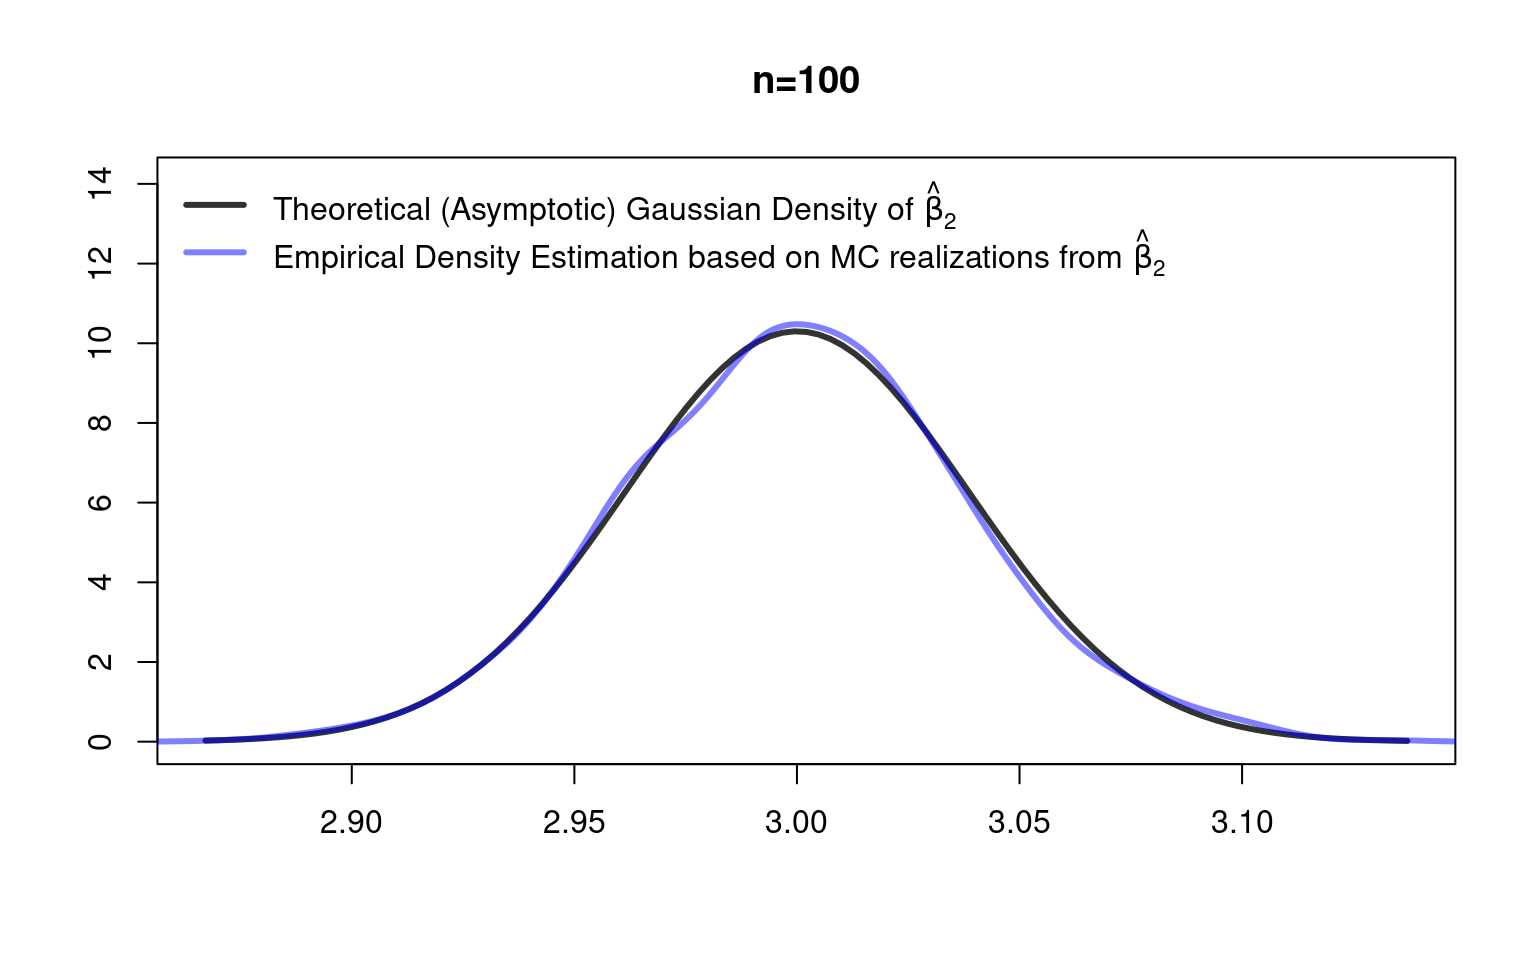
\includegraphics[width=1\textwidth]{figure/minimal-unnamed-chunk-82-1} \end{center}

Great! The nonparametric density estimation (estimated via \texttt{density()}) computed from the simulated realizations of \(\hat\beta_2\) is indicating that \(\hat\beta_2\) is really normally distributed as described by our theoretical result in Theorem \ref{OLSnormality1} (homoscedastic case) and in Equation \eqref{OLSnormality1Rob} (heteroscedastic case).

However, is the asymptotic distribution of \(\hat\beta_2\) also usable for (very) small samples like \(n=5\)? Let's check that:

\begin{Shaded}
\begin{Highlighting}[]
\FunctionTok{set.seed}\NormalTok{(}\DecValTok{123}\NormalTok{)}
\NormalTok{n           }\OtherTok{\textless{}{-}} \DecValTok{5}       \CommentTok{\# a small sample size}
\NormalTok{beta\_true   }\OtherTok{\textless{}{-}} \FunctionTok{c}\NormalTok{(}\DecValTok{2}\NormalTok{,}\DecValTok{3}\NormalTok{,}\DecValTok{4}\NormalTok{) }\CommentTok{\# true data vector}

\DocumentationTok{\#\# Mean and variance of the true asymptotic }
\DocumentationTok{\#\# normal distribution of beta\_hat\_2:}
\CommentTok{\# true mean}
\NormalTok{beta\_true\_2     }\OtherTok{\textless{}{-}}\NormalTok{ beta\_true[}\DecValTok{2}\NormalTok{] }
\CommentTok{\# true variance}
\NormalTok{var\_true\_beta\_2 }\OtherTok{\textless{}{-}}\NormalTok{ (}\FunctionTok{solve}\NormalTok{(}\FunctionTok{diag}\NormalTok{(}\FunctionTok{c}\NormalTok{(}\DecValTok{1}\NormalTok{, }\DecValTok{16}\SpecialCharTok{/}\DecValTok{3}\NormalTok{, }\DecValTok{25}\SpecialCharTok{/}\DecValTok{3}\NormalTok{)))}\SpecialCharTok{\%*\%} 
                          \FunctionTok{diag}\NormalTok{(}\FunctionTok{c}\NormalTok{(}\DecValTok{4}\SpecialCharTok{/}\DecValTok{9}\NormalTok{, }\DecValTok{64}\SpecialCharTok{/}\DecValTok{15}\NormalTok{, }\DecValTok{100}\SpecialCharTok{/}\DecValTok{27}\NormalTok{))}\SpecialCharTok{\%*\%} 
                    \FunctionTok{solve}\NormalTok{(}\FunctionTok{diag}\NormalTok{(}\FunctionTok{c}\NormalTok{(}\DecValTok{1}\NormalTok{, }\DecValTok{16}\SpecialCharTok{/}\DecValTok{3}\NormalTok{, }\DecValTok{25}\SpecialCharTok{/}\DecValTok{3}\NormalTok{))))[}\DecValTok{2}\NormalTok{,}\DecValTok{2}\NormalTok{]}\SpecialCharTok{/}\NormalTok{n}

\DocumentationTok{\#\# Let\textquotesingle{}s generate 5000 realizations from beta\_hat\_2, and check }
\DocumentationTok{\#\# whether their distribution is close to the true normal }
\DocumentationTok{\#\# distribution.}
\DocumentationTok{\#\# (We don\textquotesingle{}t condition on X since the theoretical limit }
\DocumentationTok{\#\# distribution is unconditional on X)}
\NormalTok{rep        }\OtherTok{\textless{}{-}} \DecValTok{5000} \CommentTok{\# MC replications}
\NormalTok{beta\_hat\_2 }\OtherTok{\textless{}{-}} \FunctionTok{rep}\NormalTok{(}\ConstantTok{NA}\NormalTok{, }\AttributeTok{times=}\NormalTok{rep)}
\DocumentationTok{\#\#}
\ControlFlowTok{for}\NormalTok{(r }\ControlFlowTok{in} \DecValTok{1}\SpecialCharTok{:}\NormalTok{rep)\{}
\NormalTok{    MC\_data }\OtherTok{\textless{}{-}} \FunctionTok{myDataGenerator}\NormalTok{(}\AttributeTok{n    =}\NormalTok{ n, }
                               \AttributeTok{beta =}\NormalTok{ beta\_true)}
\NormalTok{    lm\_obj        }\OtherTok{\textless{}{-}} \FunctionTok{lm}\NormalTok{(Y }\SpecialCharTok{\textasciitilde{}}\NormalTok{ X\_2 }\SpecialCharTok{+}\NormalTok{ X\_3, }\AttributeTok{data =}\NormalTok{ MC\_data)}
\NormalTok{    beta\_hat\_2[r] }\OtherTok{\textless{}{-}} \FunctionTok{coef}\NormalTok{(lm\_obj)[}\DecValTok{2}\NormalTok{]}
\NormalTok{\}}

\DocumentationTok{\#\# Compare:}
\DocumentationTok{\#\# True beta\_2 versus average of beta\_hat\_2 estimates}
\NormalTok{beta\_true\_2}
\CommentTok{\#\textgreater{} [1] 3}
\FunctionTok{round}\NormalTok{(}\FunctionTok{mean}\NormalTok{(beta\_hat\_2), }\DecValTok{3}\NormalTok{)}
\CommentTok{\#\textgreater{} [1] 2.996}
\DocumentationTok{\#\# True variance of beta\_hat\_2 versus }
\DocumentationTok{\#\# empirical variance of beta\_hat\_2 estimates}
\FunctionTok{round}\NormalTok{(var\_true\_beta\_2, }\DecValTok{5}\NormalTok{)}
\CommentTok{\#\textgreater{} [1] 0.03}
\FunctionTok{round}\NormalTok{(}\FunctionTok{var}\NormalTok{(beta\_hat\_2), }\DecValTok{5}\NormalTok{)}
\CommentTok{\#\textgreater{} [1] 0.05621}

\DocumentationTok{\#\# True normal distribution of beta\_hat\_2 versus }
\DocumentationTok{\#\# empirical density of beta\_hat\_2 estimates}
\FunctionTok{library}\NormalTok{(}\StringTok{"scales"}\NormalTok{)}
\FunctionTok{curve}\NormalTok{(}\AttributeTok{expr =} \FunctionTok{dnorm}\NormalTok{(x, }\AttributeTok{mean =}\NormalTok{ beta\_true\_2, }
                   \AttributeTok{sd=}\FunctionTok{sqrt}\NormalTok{(var\_true\_beta\_2)), }
      \AttributeTok{xlab=}\StringTok{""}\NormalTok{,}\AttributeTok{ylab=}\StringTok{""}\NormalTok{, }\AttributeTok{col=}\FunctionTok{gray}\NormalTok{(.}\DecValTok{2}\NormalTok{), }\AttributeTok{lwd=}\DecValTok{3}\NormalTok{, }\AttributeTok{lty=}\DecValTok{1}\NormalTok{, }
\AttributeTok{xlim=}\FunctionTok{c}\NormalTok{(}\DecValTok{2}\NormalTok{,}\DecValTok{4}\NormalTok{), }\AttributeTok{ylim=}\FunctionTok{c}\NormalTok{(}\DecValTok{0}\NormalTok{,}\DecValTok{3}\NormalTok{),}\AttributeTok{main=}\FunctionTok{paste0}\NormalTok{(}\StringTok{"n="}\NormalTok{,n))}
\FunctionTok{lines}\NormalTok{(}\FunctionTok{density}\NormalTok{(beta\_hat\_2, }\AttributeTok{bw =} \FunctionTok{bw.SJ}\NormalTok{(beta\_hat\_2)), }
      \AttributeTok{col=}\FunctionTok{alpha}\NormalTok{(}\StringTok{"blue"}\NormalTok{,.}\DecValTok{5}\NormalTok{), }\AttributeTok{lwd=}\DecValTok{3}\NormalTok{)}
\FunctionTok{legend}\NormalTok{(}\StringTok{"topleft"}\NormalTok{, }\AttributeTok{lty=}\FunctionTok{c}\NormalTok{(}\DecValTok{1}\NormalTok{,}\DecValTok{1}\NormalTok{), }\AttributeTok{lwd=}\FunctionTok{c}\NormalTok{(}\DecValTok{3}\NormalTok{,}\DecValTok{3}\NormalTok{), }
     \AttributeTok{col=}\FunctionTok{c}\NormalTok{(}\FunctionTok{gray}\NormalTok{(.}\DecValTok{2}\NormalTok{), }\FunctionTok{alpha}\NormalTok{(}\StringTok{"blue"}\NormalTok{,.}\DecValTok{5}\NormalTok{)), }\AttributeTok{bty=}\StringTok{"n"}\NormalTok{, }\AttributeTok{legend=} 
\FunctionTok{c}\NormalTok{(}\FunctionTok{expression}\NormalTok{(}
  \StringTok{"Theoretical (Asymptotic) Gaussian Density of"}\SpecialCharTok{\textasciitilde{}}\FunctionTok{hat}\NormalTok{(beta)[}\DecValTok{2}\NormalTok{]), }
  \FunctionTok{expression}\NormalTok{(}
  \StringTok{"Empirical Density Estimation based on MC realizations from"}\SpecialCharTok{\textasciitilde{}}
  \FunctionTok{hat}\NormalTok{(beta)[}\DecValTok{2}\NormalTok{])))}
\end{Highlighting}
\end{Shaded}

\begin{center}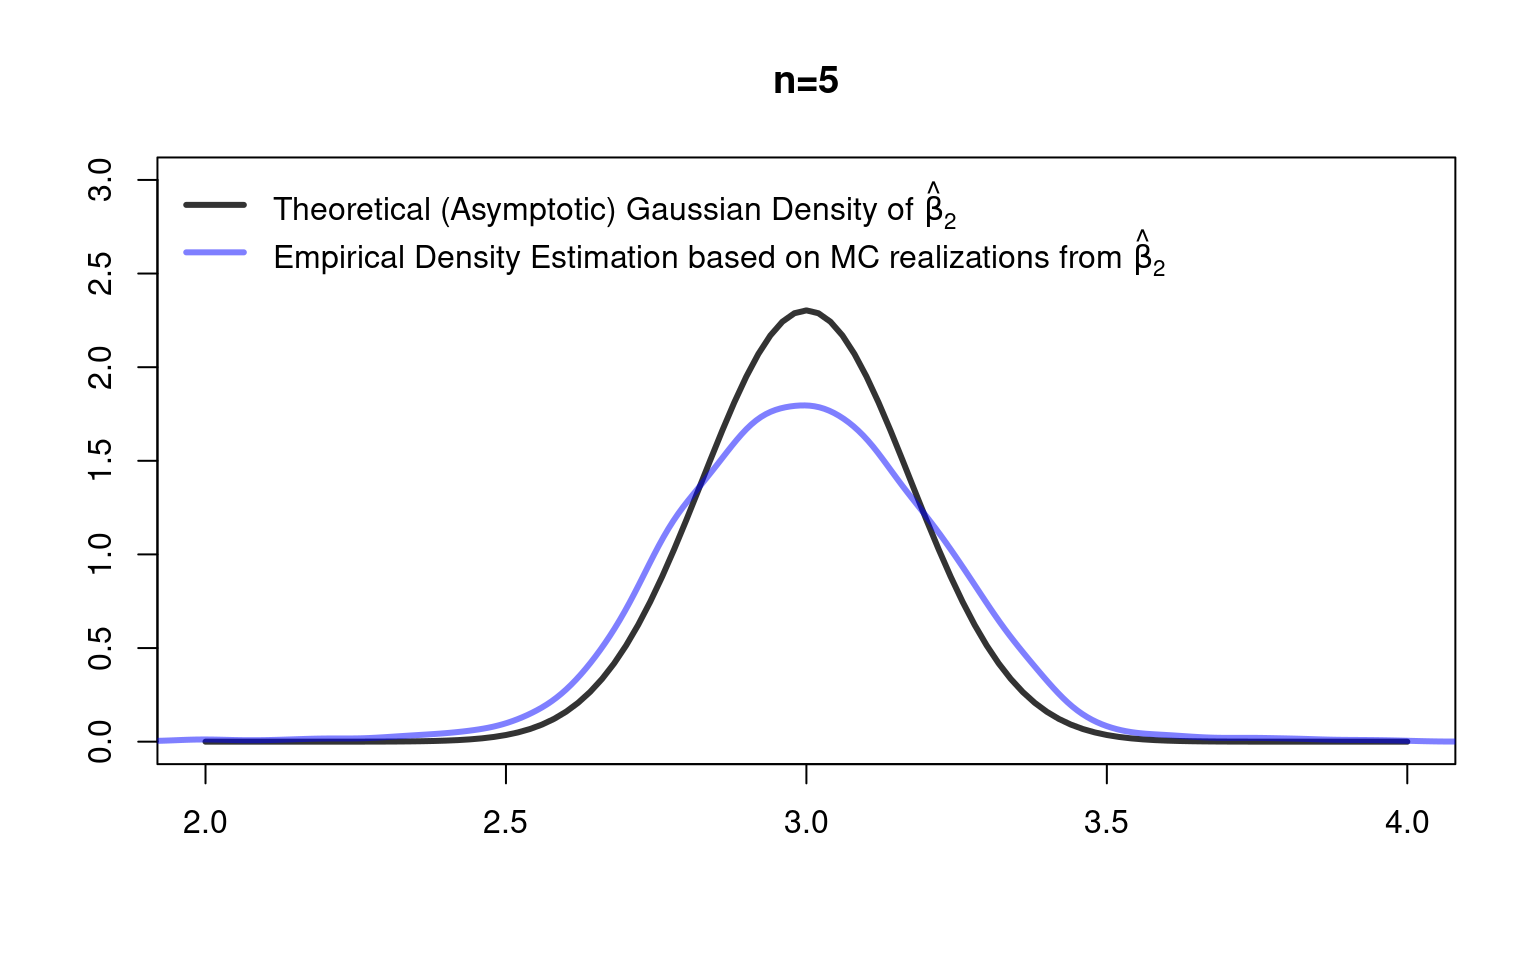
\includegraphics[width=1\textwidth]{figure/minimal-unnamed-chunk-83-1} \end{center}

Not good. The actual distribution has substantially fatter tails. That is, if we would use the quantiles of the asymptotic distribution, we would falsely reject the null-hypothesis too often (probability of type I errors would be larger than the significance level). But asymptotic are kicking in pretty fast here: things become much more reliable already for \(n=10\).

\hypertarget{testing-multiple-and-single-parameters}{%
\subsection{Testing Multiple and Single Parameters}\label{testing-multiple-and-single-parameters}}

In the following, we do inference about multiple parameters. We test
\begin{align*}
H_0:&\beta_2=3\quad\text{and}\quad\beta_3=5\\
\text{versus}\quad H_A:&\beta_2\neq 3\quad\text{and/or}\quad\beta_3\neq 5.
\end{align*}
Or equivalently
\begin{align*}
H_0:&R\beta -r = 0 \\
H_A:&R\beta -r \neq 0,
\end{align*}
where
\[
R=\left(
\begin{matrix}
0&1&0\\
0&0&1\\
\end{matrix}\right)\quad\text{ and }\quad 
r=\left(\begin{matrix}3\\5\\\end{matrix}\right).
\]
The following \(\textsf{R}\) code can be used to test this hypothesis:

\begin{Shaded}
\begin{Highlighting}[]
\FunctionTok{suppressMessages}\NormalTok{(}\FunctionTok{library}\NormalTok{(}\StringTok{"car"}\NormalTok{)) }\CommentTok{\# for linearHyothesis()}
\CommentTok{\# ?linearHypothesis}
\FunctionTok{library}\NormalTok{(}\StringTok{"sandwich"}\NormalTok{)}

\DocumentationTok{\#\# Generate data}
\NormalTok{MC\_data }\OtherTok{\textless{}{-}} \FunctionTok{myDataGenerator}\NormalTok{(}\AttributeTok{n    =} \DecValTok{100}\NormalTok{, }
                           \AttributeTok{beta =}\NormalTok{ beta\_true)}

\DocumentationTok{\#\# Estimate the linear regression model parameters}
\NormalTok{lm\_obj }\OtherTok{\textless{}{-}} \FunctionTok{lm}\NormalTok{(Y }\SpecialCharTok{\textasciitilde{}}\NormalTok{ X\_2 }\SpecialCharTok{+}\NormalTok{ X\_3, }\AttributeTok{data =}\NormalTok{ MC\_data)}

\NormalTok{vcovHC3\_mat }\OtherTok{\textless{}{-}}\NormalTok{ sandwich}\SpecialCharTok{::}\FunctionTok{vcovHC}\NormalTok{(lm\_obj, }\AttributeTok{type=}\StringTok{"HC3"}\NormalTok{)}

\DocumentationTok{\#\# Option 1:}
\NormalTok{car}\SpecialCharTok{::}\FunctionTok{linearHypothesis}\NormalTok{(}\AttributeTok{model =}\NormalTok{ lm\_obj, }
                      \AttributeTok{hypothesis.matrix =} \FunctionTok{c}\NormalTok{(}\StringTok{"X\_2=3"}\NormalTok{, }\StringTok{"X\_3=5"}\NormalTok{), }
                      \AttributeTok{vcov=}\NormalTok{vcovHC3\_mat)}
\CommentTok{\#\textgreater{} Linear hypothesis test}
\CommentTok{\#\textgreater{} }
\CommentTok{\#\textgreater{} Hypothesis:}
\CommentTok{\#\textgreater{} X\_2 = 3}
\CommentTok{\#\textgreater{} X\_3 = 5}
\CommentTok{\#\textgreater{} }
\CommentTok{\#\textgreater{} Model 1: restricted model}
\CommentTok{\#\textgreater{} Model 2: Y \textasciitilde{} X\_2 + X\_3}
\CommentTok{\#\textgreater{} }
\CommentTok{\#\textgreater{} Note: Coefficient covariance matrix supplied.}
\CommentTok{\#\textgreater{} }
\CommentTok{\#\textgreater{}   Res.Df Df      F    Pr(\textgreater{}F)    }
\CommentTok{\#\textgreater{} 1     99                        }
\CommentTok{\#\textgreater{} 2     97  2 1150.4 \textless{} 2.2e{-}16 ***}
\CommentTok{\#\textgreater{} {-}{-}{-}}
\CommentTok{\#\textgreater{} Signif. codes:  0 \textquotesingle{}***\textquotesingle{} 0.001 \textquotesingle{}**\textquotesingle{} 0.01 \textquotesingle{}*\textquotesingle{} 0.05 \textquotesingle{}.\textquotesingle{} 0.1 \textquotesingle{} \textquotesingle{} 1}

\DocumentationTok{\#\# Option 2:}
\NormalTok{R }\OtherTok{\textless{}{-}} \FunctionTok{rbind}\NormalTok{(}\FunctionTok{c}\NormalTok{(}\DecValTok{0}\NormalTok{,}\DecValTok{1}\NormalTok{,}\DecValTok{0}\NormalTok{),}
           \FunctionTok{c}\NormalTok{(}\DecValTok{0}\NormalTok{,}\DecValTok{0}\NormalTok{,}\DecValTok{1}\NormalTok{))}
\NormalTok{car}\SpecialCharTok{::}\FunctionTok{linearHypothesis}\NormalTok{(}\AttributeTok{model =}\NormalTok{ lm\_obj, }
                      \AttributeTok{hypothesis.matrix =}\NormalTok{ R, }
                      \AttributeTok{rhs =} \FunctionTok{c}\NormalTok{(}\DecValTok{3}\NormalTok{,}\DecValTok{5}\NormalTok{),}
                      \AttributeTok{vcov=}\NormalTok{vcovHC3\_mat)}
\CommentTok{\#\textgreater{} Linear hypothesis test}
\CommentTok{\#\textgreater{} }
\CommentTok{\#\textgreater{} Hypothesis:}
\CommentTok{\#\textgreater{} X\_2 = 3}
\CommentTok{\#\textgreater{} X\_3 = 5}
\CommentTok{\#\textgreater{} }
\CommentTok{\#\textgreater{} Model 1: restricted model}
\CommentTok{\#\textgreater{} Model 2: Y \textasciitilde{} X\_2 + X\_3}
\CommentTok{\#\textgreater{} }
\CommentTok{\#\textgreater{} Note: Coefficient covariance matrix supplied.}
\CommentTok{\#\textgreater{} }
\CommentTok{\#\textgreater{}   Res.Df Df      F    Pr(\textgreater{}F)    }
\CommentTok{\#\textgreater{} 1     99                        }
\CommentTok{\#\textgreater{} 2     97  2 1150.4 \textless{} 2.2e{-}16 ***}
\CommentTok{\#\textgreater{} {-}{-}{-}}
\CommentTok{\#\textgreater{} Signif. codes:  0 \textquotesingle{}***\textquotesingle{} 0.001 \textquotesingle{}**\textquotesingle{} 0.01 \textquotesingle{}*\textquotesingle{} 0.05 \textquotesingle{}.\textquotesingle{} 0.1 \textquotesingle{} \textquotesingle{} 1}
\end{Highlighting}
\end{Shaded}

The \(p\)-value is very small and allows us to reject the (false) null-hypothesis at any of the usual significance levels.

Next, we do inference about a single parameter. We test
\begin{align*}
H_0:&\beta_3=5\\
\text{versus}\quad H_A:&\beta_3\neq 5.
\end{align*}

\begin{Shaded}
\begin{Highlighting}[]
\CommentTok{\# Load libraries}
\FunctionTok{library}\NormalTok{(}\StringTok{"lmtest"}\NormalTok{)   }\CommentTok{\# for coeftest()}
\FunctionTok{library}\NormalTok{(}\StringTok{"sandwich"}\NormalTok{) }\CommentTok{\# for vcovHC()}

\DocumentationTok{\#\# Generate data}
\NormalTok{n }\OtherTok{\textless{}{-}} \DecValTok{100}
\NormalTok{MC\_data }\OtherTok{\textless{}{-}} \FunctionTok{myDataGenerator}\NormalTok{(}\AttributeTok{n    =}\NormalTok{ n, }
                           \AttributeTok{beta =}\NormalTok{ beta\_true)}

\DocumentationTok{\#\# Estimate the linear regression model parameters}
\NormalTok{lm\_obj }\OtherTok{\textless{}{-}} \FunctionTok{lm}\NormalTok{(Y }\SpecialCharTok{\textasciitilde{}}\NormalTok{ X\_2 }\SpecialCharTok{+}\NormalTok{ X\_3, }\AttributeTok{data =}\NormalTok{ MC\_data)}

\DocumentationTok{\#\# Robust t test}

\DocumentationTok{\#\# Robust standard error for \textbackslash{}hat\{\textbackslash{}beta\}\_3:}
\NormalTok{SE\_rob }\OtherTok{\textless{}{-}} \FunctionTok{sqrt}\NormalTok{(}\FunctionTok{vcovHC}\NormalTok{(lm\_obj, }\AttributeTok{type =} \StringTok{"HC3"}\NormalTok{)[}\DecValTok{3}\NormalTok{,}\DecValTok{3}\NormalTok{])}
\DocumentationTok{\#\# hypothetical (H0) value of \textbackslash{}beta\_3:}
\NormalTok{beta\_3\_H0 }\OtherTok{\textless{}{-}} \DecValTok{5}
\DocumentationTok{\#\# estimate for beta\_3:}
\NormalTok{beta\_3\_hat }\OtherTok{\textless{}{-}} \FunctionTok{coef}\NormalTok{(lm\_obj)[}\DecValTok{3}\NormalTok{]}
\DocumentationTok{\#\# robust t{-}test statistic}
\NormalTok{t\_test\_stat }\OtherTok{\textless{}{-}}\NormalTok{ (beta\_3\_hat }\SpecialCharTok{{-}}\NormalTok{ beta\_3\_H0)}\SpecialCharTok{/}\NormalTok{SE\_rob}
\DocumentationTok{\#\# p{-}value}
\NormalTok{K }\OtherTok{\textless{}{-}} \FunctionTok{length}\NormalTok{(}\FunctionTok{coef}\NormalTok{(lm\_obj))}
\DocumentationTok{\#\#}
\NormalTok{p\_value }\OtherTok{\textless{}{-}} \DecValTok{2} \SpecialCharTok{*} \FunctionTok{min}\NormalTok{(   }\FunctionTok{pt}\NormalTok{(}\AttributeTok{q =}\NormalTok{ t\_test\_stat, }\AttributeTok{df =}\NormalTok{ n }\SpecialCharTok{{-}}\NormalTok{ K), }
                   \DecValTok{1}\SpecialCharTok{{-}} \FunctionTok{pt}\NormalTok{(}\AttributeTok{q =}\NormalTok{ t\_test\_stat, }\AttributeTok{df =}\NormalTok{ n }\SpecialCharTok{{-}}\NormalTok{ K))}
\NormalTok{p\_value}
\CommentTok{\#\textgreater{} [1] 4.330845e{-}65}
\end{Highlighting}
\end{Shaded}

Again, the \(p\)-value is very small and allows us to reject the (false) null-hypothesis at any of the usual significance levels.

\hypertarget{ivr}{%
\chapter{Instrumental Variables Regression}\label{ivr}}

The current version of this chapter is basically completly taken from the free online book: \url{www.econometrics-with-r.org} \citep{Hanck_et_al_2019}

\bigskip

Regression models may suffer from problems like omitted variables, measurement errors and simultaneous causality. If so, the error term \(\eps_i\) is correlated with the regressor, \(X_{ik}\) say, and the corresponding coefficient of interest, \(\beta_k\), is estimated \textbf{inconsistently}. If one is lucky, one can add, for instance, the omitted variables to the regression to mitigate the risk of biased estimations (\say{omitted variables bias}). However, if omitted variables cannot be measured or are not available for other reasons, multiple regression cannot solve the problem. The same issue arises if there is \say{simultaneous causality}. When causality runs from \(X\) to \(Y\) \emph{and vice versa} (e.g.~if \(Y=\text{Demanded quantity of a good}\) and \(X=\text{Price of this good}\)), there will be an estimation bias that cannot be corrected for by multiple regression.

A general technique for obtaining a consistent estimator of the coefficient of interest is instrumental variables (IV) regression. In this chapter we focus on the IV regression tool called \emph{two-stage least squares} (TSLS). The first sections briefly recap the general mechanics and assumptions of IV regression and show how to perform TSLS estimation using \textsf{R}. Next, IV regression is used for estimating the elasticity of the demand for cigarettes --- a classical example where multiple regression fails to do the job because of simultaneous causality.

\hypertarget{TIVEWASRAASI}{%
\section{The IV Estimator with a Single Regressor and a Single Instrument}\label{TIVEWASRAASI}}

Consider the simple regression model
\begin{align}
  Y_i = \beta_1 + \beta_2 X_i + \eps_i \ \ , \ \ i=1,\dots,n, \label{eq:srm12}
\end{align}
where the error term \(\eps_i\) is correlated with the regressor \(X_i\) (\(X\) is the called \say{\textit{endogenous}}). In this case Assumption 2 is violated, that is, strict exogeneity and orthogonality between \(X_i\) and \(\eps_i\) do not hold. Therefore, OLS estimation (also maximum likelihood and methods of moments estimation) is inconsistent for the true \(\beta_2\). In the most simple case, IV regression uses a single instrumental variable \(Z_i\) to obtain a consistent estimator for \(\beta_2\).

\paragraph*{Conditions for valid instruments:}

\(Z_i\) must satisfy two conditions to be a valid instrument:

\begin{enumerate}
\item \textbf{Instrument relevance condition:}\\
$X_i$ and its instrument $Z_i$ \emph{must be} correlated: $\rho_{Z,X} \neq 0$.
\item \textbf{Instrument exogeneity condition:}\\
$E(\eps_i|Z_i)=0$. As a consequence: The instrument $Z_i$ \emph{must not be} correlated with the error term $\eps_i$: $\rho_{Z,\eps} = 0$.
\end{enumerate}

\hypertarget{the-two-stage-least-squares-estimator}{%
\subsection{The Two-Stage Least Squares Estimator}\label{the-two-stage-least-squares-estimator}}

As can be guessed from its name, TSLS proceeds in two stages. In the first stage, the variation in the endogenous regressor \(X_i\) is decomposed into a \say{problem-free} component that is explained by the (exogenous) instrument \(Z_i\) and a problematic component that is correlated with the error \(\eps_i\). The second stage uses the problem-free component of the variation in \(X_i\) to estimate \(\beta_2\).

The first stage regression model is
\[
X_i = \pi_0 + \pi_1 Z_i + \nu_i,
\]
where \(\pi_0 + \pi_1 Z_i\) is the component of \(X_i\) that is explained by \(Z_i\) while \(\nu_i\) is the component (an error term) that cannot be explained by \(Z_i\) and exhibits correlation with \(\eps_i\).

Using the OLS estimates \(\widehat{\pi}_0\) and \(\widehat{\pi}_1\) we obtain predicted values \(\widehat{X}_i=\hat\pi_0+\hat\pi_1 Z_i,\ i=1,\dots,n\). If \(Z_i\) is a valid instrument, the \(\widehat{X}_i\) are problem-free in the sense that \(\widehat{X}_i\) is \textbf{exogenous} in a regression of \(Y_i\) on \(\widehat{X}_i\) which is done in the second stage regression. The second stage produces \(\widehat{\beta}_1^{TSLS}\) and \(\widehat{\beta}_2^{TSLS}\), the TSLS estimates of \(\beta_1\) and \(\beta_2\).

For the case of a single instrument one can show that the TSLS estimator of \(\beta_2\) is
\begin{align}
\widehat{\beta}_2^{TSLS} = \frac{s_{ZY}}{s_{ZX}} = \frac{\frac{1}{n-1}\sum_{i=1}^n(Y_i - \overline{Y})(Z_i - \overline{Z})}{\frac{1}{n-1}\sum_{i=1}^n(X_i - \overline{X})(Z_i - \overline{Z})}, \label{eq:simpletsls}
\end{align}
which is nothing but the ratio of the sample covariance between \(Z_i\) and \(Y_i\) to the sample covariance between \(Z_i\) and \(X_i\).

The estimator in \eqref{eq:simpletsls} is a consistent estimator for \(\beta_2\) in \eqref{eq:srm12} under the assumption that \(Z_i\) is a valid instrument. The CLT implies that the distribution of \(\widehat{\beta}_2^{TSLS}\) can be approximated by a normal distribution if the sample size \(n\) is large. This allows us to use \(t\)-statistics, \(F\)-statistics, confidence intervals, etc.

\hypertarget{application-demand-for-cigarettes-12}{%
\subsection{Application: Demand For Cigarettes (1/2)}\label{application-demand-for-cigarettes-12}}

The relation between the demand for and the price of commodities is a simple yet widespread problem in economics. Health economics is concerned with the study of how health-affecting behavior of individuals is influenced by the health-care system and regulation policy. Probably the most prominent example in public policy debates is smoking as it is related to many illnesses and negative externalities.

It is plausible that cigarette consumption can be reduced by taxing cigarettes more heavily. The question is by \emph{how much} taxes must be increased to reach a certain reduction in cigarette consumption. Economists use elasticities to answer this kind of question. Since the price elasticity for the demand of cigarettes is unknown, it must be estimated. A simple OLS regression of log quantity on log price cannot be used to estimate the effect of interest since there is simultaneous causality between demand and supply. Instead, IV regression can be used.

We use the data set \texttt{CigarettesSW} which comes with the package \texttt{AER}. It is a panel data set that contains observations on cigarette consumption and several economic indicators for all 48 continental federal states of the U.S. from 1985 to 1995. In the following, however, we consider data for the cross section of states in 1995 only -- that is, we transform the panel data to a cross-sectional data set. We start by loading the package, attaching the data set. An overview about summary statistics for each of the variables is returned by \texttt{summary(CigarettesSW)}. Use \texttt{?CigarettesSW} for a detailed description of the variables.

\begin{Shaded}
\begin{Highlighting}[]
\CommentTok{\# load the data set and get an overview}
\FunctionTok{library}\NormalTok{(}\StringTok{"AER"}\NormalTok{)}
\FunctionTok{data}\NormalTok{(}\StringTok{"CigarettesSW"}\NormalTok{)}
\FunctionTok{summary}\NormalTok{(CigarettesSW)}
\end{Highlighting}
\end{Shaded}

\begin{verbatim}
#>      state      year         cpi          population           packs       
#>  AL     : 2   1985:48   Min.   :1.076   Min.   :  478447   Min.   : 49.27  
#>  AR     : 2   1995:48   1st Qu.:1.076   1st Qu.: 1622606   1st Qu.: 92.45  
#>  AZ     : 2             Median :1.300   Median : 3697472   Median :110.16  
#>  CA     : 2             Mean   :1.300   Mean   : 5168866   Mean   :109.18  
#>  CO     : 2             3rd Qu.:1.524   3rd Qu.: 5901500   3rd Qu.:123.52  
#>  CT     : 2             Max.   :1.524   Max.   :31493524   Max.   :197.99  
#>  (Other):84                                                                
#>      income               tax            price             taxs       
#>  Min.   :  6887097   Min.   :18.00   Min.   : 84.97   Min.   : 21.27  
#>  1st Qu.: 25520384   1st Qu.:31.00   1st Qu.:102.71   1st Qu.: 34.77  
#>  Median : 61661644   Median :37.00   Median :137.72   Median : 41.05  
#>  Mean   : 99878736   Mean   :42.68   Mean   :143.45   Mean   : 48.33  
#>  3rd Qu.:127313964   3rd Qu.:50.88   3rd Qu.:176.15   3rd Qu.: 59.48  
#>  Max.   :771470144   Max.   :99.00   Max.   :240.85   Max.   :112.63  
#> 
\end{verbatim}

We are interested in estimating \(\beta_2\) in
\begin{align}
  \log(Q_i^{cigarettes}) = \beta_1 + \beta_2 \log(P_i^{cigarettes}) + \eps_i, \label{eq:cigstsls}
\end{align}
where \(Q_i^{cigarettes}\) is the number of cigarette packs per capita sold and \(P_i^{cigarettes}\) is the after-tax average real price per pack of cigarettes in state \(i=1,\dots,n=48\).

The instrumental variable we are going to use for instrumenting the endogenous regressor \(\log(P_i^{cigarettes})\) is \(SalesTax\), the portion of taxes on cigarettes arising from the general sales tax. \(SalesTax\) is measured in dollars per pack. The idea is that:

\begin{enumerate}
\item $SalesTax$ is a relevant instrument as it is included in the after-tax average price per pack. 
\item Also, it is plausible that $SalesTax$ is exogenous since the sales tax does not influence quantity sold directly but indirectly through the price.
\end{enumerate}

In the following, we perform some transformations in order to obtain deflated cross section data for the year 1995. We also compute the sample correlation between the sales tax and price per pack. The sample correlation is a consistent estimator of the population correlation. The estimate of approximately \(0.614\) indicates that \(SalesTax\) and \(P_i^{cigarettes}\) exhibit positive correlation which meets our expectations: higher sales taxes lead to higher prices. However, a correlation analysis like this is not sufficient for checking whether the instrument is relevant. We will later come back to the issue of checking whether an instrument is relevant and exogenous; see Chapter \ref{civ}.

\begin{Shaded}
\begin{Highlighting}[]
\CommentTok{\# compute real per capita prices}
\NormalTok{CigarettesSW}\SpecialCharTok{$}\NormalTok{rprice }\OtherTok{\textless{}{-}} \FunctionTok{with}\NormalTok{(CigarettesSW, price }\SpecialCharTok{/}\NormalTok{ cpi)}

\CommentTok{\#  compute the sales tax}
\NormalTok{CigarettesSW}\SpecialCharTok{$}\NormalTok{salestax }\OtherTok{\textless{}{-}} \FunctionTok{with}\NormalTok{(CigarettesSW, (taxs }\SpecialCharTok{{-}}\NormalTok{ tax) }\SpecialCharTok{/}\NormalTok{ cpi)}

\CommentTok{\# check the correlation between sales tax and price}
\FunctionTok{cor}\NormalTok{(CigarettesSW}\SpecialCharTok{$}\NormalTok{salestax, CigarettesSW}\SpecialCharTok{$}\NormalTok{price)}
\CommentTok{\#\textgreater{} [1] 0.6141228}

\CommentTok{\# generate a subset for the year 1995}
\NormalTok{c1995 }\OtherTok{\textless{}{-}} \FunctionTok{subset}\NormalTok{(CigarettesSW, year }\SpecialCharTok{==} \StringTok{"1995"}\NormalTok{)}
\end{Highlighting}
\end{Shaded}

The first stage regression is
\[
\log(P_i^{cigarettes}) = \pi_0 + \pi_1 SalesTax_i + \nu_i.
\]
We estimate this model in \textsf{R} using \texttt{lm()}. In the second stage we run a regression of \(\log(Q_i^{cigarettes})\) on \(\widehat{\log(P_i^{cigarettes})}\) to obtain \(\widehat{\beta}_1^{TSLS}\) and \(\widehat{\beta}_2^{TSLS}\).

\begin{Shaded}
\begin{Highlighting}[]
\CommentTok{\# perform the first stage regression}
\NormalTok{cig\_s1 }\OtherTok{\textless{}{-}} \FunctionTok{lm}\NormalTok{(}\FunctionTok{log}\NormalTok{(rprice) }\SpecialCharTok{\textasciitilde{}}\NormalTok{ salestax, }\AttributeTok{data =}\NormalTok{ c1995)}

\FunctionTok{coeftest}\NormalTok{(cig\_s1, }\AttributeTok{vcov =}\NormalTok{ vcovHC, }\AttributeTok{type =} \StringTok{"HC1"}\NormalTok{)}
\CommentTok{\#\textgreater{} }
\CommentTok{\#\textgreater{} t test of coefficients:}
\CommentTok{\#\textgreater{} }
\CommentTok{\#\textgreater{}              Estimate Std. Error  t value  Pr(\textgreater{}|t|)    }
\CommentTok{\#\textgreater{} (Intercept) 4.6165463  0.0289177 159.6444 \textless{} 2.2e{-}16 ***}
\CommentTok{\#\textgreater{} salestax    0.0307289  0.0048354   6.3549 8.489e{-}08 ***}
\CommentTok{\#\textgreater{} {-}{-}{-}}
\CommentTok{\#\textgreater{} Signif. codes:  0 \textquotesingle{}***\textquotesingle{} 0.001 \textquotesingle{}**\textquotesingle{} 0.01 \textquotesingle{}*\textquotesingle{} 0.05 \textquotesingle{}.\textquotesingle{} 0.1 \textquotesingle{} \textquotesingle{} 1}
\end{Highlighting}
\end{Shaded}

The first stage regression is
\[
\widehat{\log(P_i^{cigarettes})} = \underset{(0.03)}{4.62} + \underset{(0.005)}{0.031}\; SalesTax_i
\]
which predicts the relation between sales tax price per cigarettes to be positive. How much of the observed variation in \(\log(P^{cigarettes})\) is explained by the instrument \(SalesTax\)? This can be answered by looking at the regression's \(R^2\) which states that about \(47\%\) of the variation in after tax prices is explained by the variation of the sales tax across states.

\begin{Shaded}
\begin{Highlighting}[]
\CommentTok{\# inspect the R\^{}2 of the first stage regression}
\FunctionTok{summary}\NormalTok{(cig\_s1)}\SpecialCharTok{$}\NormalTok{r.squared}
\CommentTok{\#\textgreater{} [1] 0.4709961}
\end{Highlighting}
\end{Shaded}

We next store \(\widehat{\log(P_i^{cigarettes})}\), the fitted values obtained by the first stage regression \texttt{cig\_s1}, in the variable \texttt{lcigp\_pred}.

\begin{Shaded}
\begin{Highlighting}[]
\CommentTok{\# store the predicted values}
\NormalTok{lcigp\_pred }\OtherTok{\textless{}{-}}\NormalTok{ cig\_s1}\SpecialCharTok{$}\NormalTok{fitted.values}
\end{Highlighting}
\end{Shaded}

Next, we run the second stage regression which gives us the TSLS estimates we seek.

\begin{Shaded}
\begin{Highlighting}[]
\CommentTok{\# run the stage 2 regression}
\NormalTok{cig\_s2 }\OtherTok{\textless{}{-}} \FunctionTok{lm}\NormalTok{(}\FunctionTok{log}\NormalTok{(c1995}\SpecialCharTok{$}\NormalTok{packs) }\SpecialCharTok{\textasciitilde{}}\NormalTok{ lcigp\_pred)}
\FunctionTok{coeftest}\NormalTok{(cig\_s2, }\AttributeTok{vcov =}\NormalTok{ vcovHC, }\AttributeTok{type =} \StringTok{"HC1"}\NormalTok{)}
\CommentTok{\#\textgreater{} }
\CommentTok{\#\textgreater{} t test of coefficients:}
\CommentTok{\#\textgreater{} }
\CommentTok{\#\textgreater{}             Estimate Std. Error t value  Pr(\textgreater{}|t|)    }
\CommentTok{\#\textgreater{} (Intercept)   9.7199     1.5971  6.0859 2.153e{-}07 ***}
\CommentTok{\#\textgreater{} lcigp\_pred   {-}1.0836     0.3337 {-}3.2472  0.002178 ** }
\CommentTok{\#\textgreater{} {-}{-}{-}}
\CommentTok{\#\textgreater{} Signif. codes:  0 \textquotesingle{}***\textquotesingle{} 0.001 \textquotesingle{}**\textquotesingle{} 0.01 \textquotesingle{}*\textquotesingle{} 0.05 \textquotesingle{}.\textquotesingle{} 0.1 \textquotesingle{} \textquotesingle{} 1}
\end{Highlighting}
\end{Shaded}

Thus estimating the model \eqref{eq:cigstsls} using TSLS yields
\begin{align}
  \widehat{\log(Q_i^{cigarettes})} = \underset{(1.60)}{9.72} - \underset{(0.33)}{1.08} \widehat{\log(P_i^{cigarettes})}, \label{eq:ecigstsls}
\end{align}

The function \texttt{ivreg()} from the package \texttt{AER} carries out TSLS procedure automatically. It is used similarly as \texttt{lm()}. Instruments can be added to the usual specification of the regression formula using a vertical bar separating the model equation from the instruments. Thus, for the regression at hand the correct formula is \texttt{log(packs)\ \textasciitilde{}\ log(rprice)\ \textbar{}\ salestax}.

\begin{Shaded}
\begin{Highlighting}[]
\CommentTok{\# perform TSLS using \textquotesingle{}ivreg()\textquotesingle{}}
\NormalTok{cig\_ivreg }\OtherTok{\textless{}{-}} \FunctionTok{ivreg}\NormalTok{(}\FunctionTok{log}\NormalTok{(packs) }\SpecialCharTok{\textasciitilde{}} \FunctionTok{log}\NormalTok{(rprice) }\SpecialCharTok{|}\NormalTok{ salestax, }
                   \AttributeTok{data =}\NormalTok{ c1995)}

\FunctionTok{coeftest}\NormalTok{(cig\_ivreg, }\AttributeTok{vcov =}\NormalTok{ vcovHC, }\AttributeTok{type =} \StringTok{"HC1"}\NormalTok{)}
\CommentTok{\#\textgreater{} }
\CommentTok{\#\textgreater{} t test of coefficients:}
\CommentTok{\#\textgreater{} }
\CommentTok{\#\textgreater{}             Estimate Std. Error t value  Pr(\textgreater{}|t|)    }
\CommentTok{\#\textgreater{} (Intercept)  9.71988    1.52832  6.3598 8.346e{-}08 ***}
\CommentTok{\#\textgreater{} log(rprice) {-}1.08359    0.31892 {-}3.3977  0.001411 ** }
\CommentTok{\#\textgreater{} {-}{-}{-}}
\CommentTok{\#\textgreater{} Signif. codes:  0 \textquotesingle{}***\textquotesingle{} 0.001 \textquotesingle{}**\textquotesingle{} 0.01 \textquotesingle{}*\textquotesingle{} 0.05 \textquotesingle{}.\textquotesingle{} 0.1 \textquotesingle{} \textquotesingle{} 1}
\end{Highlighting}
\end{Shaded}

We find that the coefficient estimates coincide for both approaches.

\paragraph*{Two Notes on the Computation of TSLS Standard Errors:}
\begin{enumerate}
\item We have demonstrated that running the individual regressions for each stage of TSLS using `lm()` leads to the same coefficient estimates as when using `ivreg()`. However, the standard errors reported for the second-stage regression, e.g., by `coeftest()` or `summary()`, are \textbf{invalid}: neither adjusts for using predictions from the first-stage regression as regressors in the second-stage regression. Fortunately, `ivreg()` performs the necessary adjustment automatically. This is another advantage over manual step-by-step estimation which we have done above for demonstrating the mechanics of the procedure.
\item Just like in multiple regression it is important to compute heteroskedasticity-robust standard errors as we have done above using `vcovHC()`.
\end{enumerate}

The TSLS estimate for \(\beta_2\) in \eqref{eq:ecigstsls} suggests that an increase in cigarette prices by one percent reduces cigarette consumption by roughly \(1.08\) percentage points, which is fairly elastic. However, we should keep in mind that this estimate might not be trustworthy even though we used IV estimation: there still might be a bias due to \textbf{omitted variables}. Thus a multiple IV regression approach is needed to reduce the risk of omitted variable biases.

\hypertarget{TGIVRM}{%
\section{The General IV Regression Model}\label{TGIVRM}}

The simple IV regression model is easily extended to a multiple regression model which we refer to as the general IV regression model. In this model we distinguish between four types of variables: the dependent variable, included exogenous variables, included endogenous variables and instrumental variables:
\begin{align}
  Y_i = \beta_1 + \beta_2 X_{2i} + \dots + \beta_K X_{Ki} + \beta_{K+1} W_{1i} + \dots + \beta_{K+r} W_{ri} + \eps_i, \label{eq:givmodel}
\end{align}
with \(i=1,\dots,n\) is the general instrumental variables regression model where

\begin{itemize}
\item $Y_i$ is the dependent variable
\item $\beta_1,\dots,\beta_{K+r}$ are $K+r$ unknown regression coefficients
\item $X_{2i},\dots,X_{Ki}$ are $K-1$ endogenous regressors 
\item $W_{1i},\dots,W_{ri}$ are $r$ exogenous regressors which are uncorrelated with $\eps_i$
\item $\eps_i$ is the error term
\item $Z_{1i},\dots,Z_{mi}$ are $m$ instrumental variables
\end{itemize}
\vspace{0.5cm}

The coefficients are \textbf{overidentified} if \(m>(K-1)\). If \(m<(K-1)\), the coefficients are \textbf{underidentified} and when \(m=(K-1)\) they are \textbf{exactly identified}. For estimation of the IV regression model we require exact identification or overidentification.

Estimating regression models with TSLS using multiple instruments by means of \texttt{ivreg()} is straightforward. There are, however, some subtleties in correctly specifying the regression formula. Assume that you want to estimate the model
\[
Y_i = \beta_1 + \beta_2 X_{2i} + \beta_3 X_{3i} + \beta_4 W_{1i} + \eps_i
\]
where \(X_{2i}\) and \(X_{3i}\) are endogenous regressors that shall be instrumented by \(Z_{1i}\), \(Z_{2i}\) and \(Z_{3i}\), and where \(W_{1i}\) is an exogenous regressor. Say the corresponding data is available in a \texttt{data.frame} with column names \texttt{y}, \texttt{x2}, \texttt{x3}, \texttt{w1}, \texttt{z1}, \texttt{z2} and \texttt{z3}. It might be tempting to specify the argument \texttt{formula} in your call of \texttt{ivreg()} as \texttt{y\ \textasciitilde{}\ x2\ +\ x3\ +\ w1\ \textbar{}\ z1\ +\ z2\ +\ z3} which is, however, \textbf{wrong}. As explained in the documentation of \texttt{ivreg()} (see \texttt{?ivreg}), it is necessary to list \emph{all} exogenous variables as instruments too, that is joining them by \texttt{+}'s on the right of the vertical bar: \texttt{y\ \textasciitilde{}\ x2\ +\ x3\ +\ w1\ \textbar{}\ w1\ +\ z1\ +\ z2\ +\ z3}, where \texttt{w1} is ``instrumenting itself''.

Similarly to the simple IV regression model, the general IV model \eqref{eq:givmodel} can be estimated using the two-stage least squares estimator:

\begin{itemize}
\item \textbf{First-stage regression(s):}\\
Run an OLS regression for each of the endogenous variables ($X_{2i},\dots,X_{Ki}$) on all instrumental variables ($Z_{1i},\dots,Z_{mi}$), all exogenous variables ($W_{1i},\dots,W_{ri}$) \textbf{and an intercept}. Compute the fitted values ($\widehat{X}_{2i},\dots,\widehat{X}_{Ki}$).
\item \textbf{Second-stage regression:}\\
Regress the dependent variable on the predicted values of all endogenous regressors, all exogenous variables and an intercept using OLS. This gives $\widehat{\beta}_{1}^{TSLS},\dots,\widehat{\beta}_{K+r}^{TSLS}$, the TSLS estimates of the model coefficients.
\end{itemize}

In the general IV regression model, the instrument relevance and instrument exogeneity assumptions are equivalent to the case of the simple regression model with a single endogenous regressor and only one instrument. That is, for \(Z_{1i},\dots,Z_{mi}\) to be a set of valid instruments, the following two conditions must be fulfilled:

\begin{enumerate}
\item \textbf{Instrument Relevance}\\
If there are $K-1$ endogenous variables, $r$ exogenous variables and $m\geq K-1$ instruments and the $\widehat{X}_{2i}^*,\dots,\widehat{X}_{Ki}^*$ are the predicted values from the $K-1$ population first stage regressions, it must hold that $$(\widehat{X}_{2i}^*,\dots,\widehat{X}_{Ki}^*, W_{1i}, \dots, W_{ri},1)$$ are not perfectly multicollinear, where \say{$1$} denotes the constant regressor (intercept) which equals $1$ for all observations.\\
\textit{Explanations}:  Let's say there is only one endogenous regressor $X_i$. If all the instruments $Z_{1i},\dots,Z_{mi}$ are irrelevant, all the $\widehat{X}^*_i$ are just the mean of $X$ such that there is perfect multicollinearity with the constant intercept $1$.\\
\item \textbf{Instrument Exogeneity}\\
$E(\eps_i|Z_{1i},\dots,Z_{im})=0$. Consequently, all $m$ instruments must be uncorrelated with the error term, 
$$
\rho_{Z_{1},\eps} = 0,\dots,\rho_{Z_{m},\eps} = 0.
$$
\end{enumerate}

One can show that if the IV regression assumptions hold, the TSLS estimator in \eqref{eq:givmodel} is consistent and normally distributed when the sample size \(n\) is large. That is, if we have valid instruments, we obtain valid statistical inference using \(t\)-tests, \(F\)-tests and confidence intervals for the model coefficients.

\hypertarget{application-demand-for-cigarettes-22}{%
\subsection{Application: Demand for Cigarettes (2/2)}\label{application-demand-for-cigarettes-22}}

The estimated elasticity of the demand for cigarettes in \eqref{eq:srm12} is \(1.08\). Although \eqref{eq:srm12} was estimated using IV regression it is plausible that this IV estimate is biased. The TSLS estimator is inconsistent for the true \(\beta_2\) if the instrument (here: the real sales tax per pack) is invalid, i.e., if the instrument correlates with the error term. This is likely to be the case here since there are economic factors, like state income, which impact the demand for cigarettes and correlate with the sales tax. States with high personal income tend to generate tax revenues by income taxes and less by sales taxes. Consequently, state income should be included in the regression model.
\begin{align}
  \log(Q_i^{cigarettes}) = \beta_1 + \beta_2 \log(P_i^{cigarettes}) + \beta_3 \log(income_i) + \eps_i \label{eq:mcigstsls1}
\end{align}

Before estimating \eqref{eq:mcigstsls1} using \texttt{ivreg()} we define \(income\) as real per capita income \texttt{rincome} and append it to the data set \texttt{CigarettesSW}.

\begin{Shaded}
\begin{Highlighting}[]
\CommentTok{\# add real income to the dataset (cpi: consumer price index)}
\NormalTok{CigarettesSW}\SpecialCharTok{$}\NormalTok{rincome }\OtherTok{\textless{}{-}} \FunctionTok{with}\NormalTok{(CigarettesSW, }
\NormalTok{                             income }\SpecialCharTok{/}\NormalTok{ population }\SpecialCharTok{/}\NormalTok{ cpi)}

\NormalTok{c1995 }\OtherTok{\textless{}{-}} \FunctionTok{subset}\NormalTok{(CigarettesSW, year }\SpecialCharTok{==} \StringTok{"1995"}\NormalTok{)}
\end{Highlighting}
\end{Shaded}

\begin{Shaded}
\begin{Highlighting}[]
\CommentTok{\# estimate the model}
\NormalTok{cig\_ivreg2 }\OtherTok{\textless{}{-}} \FunctionTok{ivreg}\NormalTok{(}\FunctionTok{log}\NormalTok{(packs) }\SpecialCharTok{\textasciitilde{}} \FunctionTok{log}\NormalTok{(rprice) }\SpecialCharTok{+} 
                                 \FunctionTok{log}\NormalTok{(rincome) }\SpecialCharTok{|} \FunctionTok{log}\NormalTok{(rincome) }\SpecialCharTok{+} 
\NormalTok{                    salestax, }\AttributeTok{data =}\NormalTok{ c1995)}

\FunctionTok{coeftest}\NormalTok{(cig\_ivreg2, }\AttributeTok{vcov =}\NormalTok{ vcovHC, }\AttributeTok{type =} \StringTok{"HC1"}\NormalTok{)}
\CommentTok{\#\textgreater{} }
\CommentTok{\#\textgreater{} t test of coefficients:}
\CommentTok{\#\textgreater{} }
\CommentTok{\#\textgreater{}              Estimate Std. Error t value  Pr(\textgreater{}|t|)    }
\CommentTok{\#\textgreater{} (Intercept)   9.43066    1.25939  7.4883 1.935e{-}09 ***}
\CommentTok{\#\textgreater{} log(rprice)  {-}1.14338    0.37230 {-}3.0711  0.003611 ** }
\CommentTok{\#\textgreater{} log(rincome)  0.21452    0.31175  0.6881  0.494917    }
\CommentTok{\#\textgreater{} {-}{-}{-}}
\CommentTok{\#\textgreater{} Signif. codes:  0 \textquotesingle{}***\textquotesingle{} 0.001 \textquotesingle{}**\textquotesingle{} 0.01 \textquotesingle{}*\textquotesingle{} 0.05 \textquotesingle{}.\textquotesingle{} 0.1 \textquotesingle{} \textquotesingle{} 1}
\end{Highlighting}
\end{Shaded}

We obtain
\begin{align}
  \widehat{\log(Q_i^{cigarettes})} = \underset{(1.26)}{9.42} - \underset{(0.37)}{1.14} \log(P_i^{cigarettes}) + \underset{(0.31)}{0.21} \log(income_i). \label{eq:emcigstsls2}
\end{align}

In the following we add the cigarette-specific taxes (\(cigtax_i\)) as a further instrumental variable and estimate again using TSLS.

\begin{Shaded}
\begin{Highlighting}[]
\CommentTok{\# add cigtax to the data set}
\NormalTok{CigarettesSW}\SpecialCharTok{$}\NormalTok{cigtax }\OtherTok{\textless{}{-}} \FunctionTok{with}\NormalTok{(CigarettesSW, tax}\SpecialCharTok{/}\NormalTok{cpi)}

\NormalTok{c1995 }\OtherTok{\textless{}{-}} \FunctionTok{subset}\NormalTok{(CigarettesSW, year }\SpecialCharTok{==} \StringTok{"1995"}\NormalTok{)}
\end{Highlighting}
\end{Shaded}

\begin{Shaded}
\begin{Highlighting}[]
\CommentTok{\# estimate the model}
\NormalTok{cig\_ivreg3 }\OtherTok{\textless{}{-}} \FunctionTok{ivreg}\NormalTok{(}\FunctionTok{log}\NormalTok{(packs) }\SpecialCharTok{\textasciitilde{}} \FunctionTok{log}\NormalTok{(rprice) }\SpecialCharTok{+} \FunctionTok{log}\NormalTok{(rincome) }\SpecialCharTok{|} 
                    \FunctionTok{log}\NormalTok{(rincome) }\SpecialCharTok{+}\NormalTok{ salestax }\SpecialCharTok{+}\NormalTok{ cigtax, }
                    \AttributeTok{data =}\NormalTok{ c1995)}

\FunctionTok{coeftest}\NormalTok{(cig\_ivreg3, }\AttributeTok{vcov =}\NormalTok{ vcovHC, }\AttributeTok{type =} \StringTok{"HC1"}\NormalTok{)}
\CommentTok{\#\textgreater{} }
\CommentTok{\#\textgreater{} t test of coefficients:}
\CommentTok{\#\textgreater{} }
\CommentTok{\#\textgreater{}              Estimate Std. Error t value  Pr(\textgreater{}|t|)    }
\CommentTok{\#\textgreater{} (Intercept)   9.89496    0.95922 10.3157 1.947e{-}13 ***}
\CommentTok{\#\textgreater{} log(rprice)  {-}1.27742    0.24961 {-}5.1177 6.211e{-}06 ***}
\CommentTok{\#\textgreater{} log(rincome)  0.28040    0.25389  1.1044    0.2753    }
\CommentTok{\#\textgreater{} {-}{-}{-}}
\CommentTok{\#\textgreater{} Signif. codes:  0 \textquotesingle{}***\textquotesingle{} 0.001 \textquotesingle{}**\textquotesingle{} 0.01 \textquotesingle{}*\textquotesingle{} 0.05 \textquotesingle{}.\textquotesingle{} 0.1 \textquotesingle{} \textquotesingle{} 1}
\end{Highlighting}
\end{Shaded}

Using the two instruments \(salestax_i\) and \(cigtax_i\) we have \(m=2\) for one endogenous regressor -- so the coefficient on the endogenous regressor \(\log(P_i^{cigarettes})\) is \emph{overidentified}. The TSLS estimate of \eqref{eq:mcigstsls1} is

\begin{align}
\widehat{\log(Q_i^{cigarettes})} = \underset{(0.96)}{9.89} - \underset{(0.25)}{1.28} \log(P_i^{cigarettes}) + \underset{(0.25)}{0.28} \log(income_i). \label{eq:emcigstsls3}
\end{align}

Should we trust the estimates presented in \eqref{eq:emcigstsls2} or rather rely on \eqref{eq:emcigstsls3}? The estimates obtained using both instruments are more precise since in \eqref{eq:emcigstsls3} all standard errors reported are smaller than in \eqref{eq:emcigstsls2}. In fact, the standard error for the estimate of the demand elasticity is only two thirds of the standard error when the sales tax is the only instrument used. This is due to more information being used in estimation \eqref{eq:emcigstsls3}. \emph{If} the instruments are valid, \eqref{eq:emcigstsls3} can be considered more reliable.

However, without insights regarding the validity of the instruments it is not sensible to make such a statement. This stresses why checking instrument validity is essential. Chapter \ref{civ} briefly discusses guidelines in checking instrument validity and presents approaches that allow to test for instrument relevance and exogeneity under certain conditions. These are then used in an application to the demand for cigarettes in Chapter \ref{attdfc}.

\hypertarget{civ}{%
\section{Checking Instrument Validity}\label{civ}}

\hypertarget{instrument-relevance}{%
\subsection{Instrument Relevance}\label{instrument-relevance}}

Instruments that explain little variation in the endogenous regressor \(X_i\) are called \emph{weak instruments}. Weak instruments provide little information about the variation in \(X_i\) that is exploited by IV regression to estimate the effect of interest: the estimate of the coefficient on the endogenous regressor is estimated inaccurately. Moreover, weak instruments cause the distribution of the estimator to deviate considerably from a normal distribution even in large samples such that the usual methods for obtaining inference about the true coefficient on \(X_i\) may produce wrong results.

\paragraph*{A Rule of Thumb for Checking for Weak Instruments:}

Consider the case of a single endogenous regressor \(X_i\) and \(m\) instruments \(Z_{1i},\dots,Z_{mi}\). If the coefficients on all instruments in the population first-stage regression of a TSLS estimation are zero, the instruments do not explain any of the variation in the \(X_i\) which clearly violates assumption that instruments must be relevant. Although the latter case is unlikely to be encountered in practice, we should ask ourselves to what extent the assumption of instrument relevance should be fulfilled. While this is hard to answer for general IV regression, in the case of a \textit{single} endogenous regressor \(X_i\) one may use \textbf{the following rule of thumb}: Compute the \(F\)-statistic which corresponds to the hypothesis that the coefficients on \(Z_{1i},\dots,Z_{mi}\) are all zero in the first-stage regression. If the \(F\)-statistic is less than \(10\), the instruments are \say{weak} such that the TSLS estimate of the coefficient on \(X_i\) is probably biased and no valid statistical inference about its true value can be made.

This rule of thumb is easily implemented in \textsf{R}. Run the first-stage regression using \texttt{lm()} and subsequently compute the heteroskedasticity-robust \(F\)-statistic by means of \texttt{linearHypothesis()}. This is part of the application to the demand for cigarettes discussed in Chapter \ref{attdfc}.

\hypertarget{if-instruments-are-weak}{%
\subsubsection*{If Instruments are Weak}\label{if-instruments-are-weak}}
\addcontentsline{toc}{subsubsection}{If Instruments are Weak}

There are two ways to proceed if instruments are weak:

\begin{enumerate}
\def\labelenumi{\arabic{enumi}.}
\item
  Discard the weak instruments and/or find stronger instruments. While the former is only an option if the unknown coefficients remain identified when the weak instruments are discarded, the latter can be very difficult and even may require a redesign of the whole study.
\item
  Stick with the weak instruments but use methods that improve upon TSLS in this scenario, for example limited information maximum likelihood estimation. (Out of the scope of this course.)
\item
  Use tests that allow for inferences robust to weak instruments: \textbf{Anderson-Rubin test}
\end{enumerate}

\hypertarget{instrument-validity}{%
\subsection{Instrument Validity}\label{instrument-validity}}

If there is correlation between an instrument and the error term, IV regression is not consistent. The overidentifying restrictions test (also called the \(J\)-test) is an approach to test the hypothesis that \textbf{additional} instruments are exogenous. For the \(J\)-test to be applicable there need to be more instruments than endogenous regressors.

\paragraph*{The $J$-Statistic (or Sargan-Hansen test)}

Take \(\hat{\eps}_i^{TSLS},\ i = 1,\dots,n\), the residuals of the TSLS estimation of the general IV regression model \eqref{eq:givmodel}. Run the OLS regression
\begin{align}
\hat{\eps}_i^{TSLS} =& \delta_0 + \delta_1 Z_{1i} + \dots + \delta_m Z_{mi} + \delta_{m+1} W_{1i} + \dots + \delta_{m+r} W_{ri} + e_i \label{eq:jstatreg}
\end{align}
and test the joint hypothesis
\[
H_0: \delta_1 = \dots \delta_{m} = 0
\]
which states that all instruments are exogenous. This can be done using the corresponding \(F\)-statistic by computing
\[
J = m  F.
\]
This test is the overidentifying restrictions test and the statistic is called the \(J\)-statistic with
\[
J \overset{H_0}{\to}_d \chi^2_{m-(K-1)}\quad\text{as}\quad n\to\infty
\]
under the \textbf{assumption of homoskedasticity}. The degrees of freedom \(m-(K-1)\) state the degree of overidentification since this is the number of instruments \(m\) minus the number of endogenous regressors \(K-1\).

It is important to note that the \(J\)-statistic is only \(\chi^2_{m-(K-1)}\) distributed when the error term \(\eps_i\) in the regression \eqref{eq:jstatreg} is homoskedastic. A discussion of the heteroskedasticity-robust \(J\)-statistic is beyond the scope of this chapter. The application in the next section shows how to apply the \(J\)-test using \texttt{linearHypothesis()}.

\hypertarget{attdfc}{%
\section{Application to the Demand for Cigarettes}\label{attdfc}}

Are the general sales tax and the cigarette-specific tax valid instruments? If not, TSLS is not helpful to estimate the demand elasticity for cigarettes discussed in Chapter \ref{TGIVRM}. As discussed in Chapter \ref{TIVEWASRAASI}, both variables are likely to be relevant but whether they are exogenous is a different question.

One can argue that cigarette-specific taxes could be endogenous because there might be state specific historical factors like economic importance of the tobacco farming and cigarette production industry that lobby for low cigarette specific taxes. Since it is plausible that tobacco growing states have higher rates of smoking than others, this would lead to endogeneity of cigarette specific taxes. If we had data on the size on the tobacco and cigarette industry, we could solve this potential issue by including the information in the regression. Unfortunately, this is not the case.

However, since the role of the tobacco and cigarette industry is a factor that can be assumed to differ across states but not over time we may exploit the panel structure of \texttt{CigarettesSW}. Alternatively, a (non-panel) regression using data on \emph{changes} between two time periods eliminates such state specific and time invariant effects. Next, we consider such changes in variables between 1985 and 1995. That is, we are interested in estimating the \emph{long-run elasticity} of the demand for cigarettes.

The model to be estimated by TSLS using the general sales tax and the cigarette-specific sales tax as instruments hence is
\begin{align}
\begin{split}
  \log(Q_{i,1995}^{cigarettes}) - \log(Q_{i,1985}^{cigarettes}) =
  & \, \beta_1 + \beta_2 \left[\log(P_{i,1995}^{cigarettes}) - \log(P_{i,1985}^{cigarettes}) \right] \\ 
  &+ \beta_3 \left[\log(income_{i,1995}) - \log(income_{i,1985})\right] + \eps_i. \end{split}\label{eq:diffivreg}
\end{align}

We first create differences from 1985 to 1995 for the dependent variable, the regressors and both instruments.

\begin{Shaded}
\begin{Highlighting}[]
\CommentTok{\# subset data for year 1985}
\NormalTok{c1985 }\OtherTok{\textless{}{-}} \FunctionTok{subset}\NormalTok{(CigarettesSW, year }\SpecialCharTok{==} \StringTok{"1985"}\NormalTok{)}

\CommentTok{\# define differences in variables}
\NormalTok{packsdiff }\OtherTok{\textless{}{-}} \FunctionTok{log}\NormalTok{(c1995}\SpecialCharTok{$}\NormalTok{packs) }\SpecialCharTok{{-}} \FunctionTok{log}\NormalTok{(c1985}\SpecialCharTok{$}\NormalTok{packs)}

\NormalTok{pricediff }\OtherTok{\textless{}{-}} \FunctionTok{log}\NormalTok{(c1995}\SpecialCharTok{$}\NormalTok{price}\SpecialCharTok{/}\NormalTok{c1995}\SpecialCharTok{$}\NormalTok{cpi) }\SpecialCharTok{{-}} \FunctionTok{log}\NormalTok{(c1985}\SpecialCharTok{$}\NormalTok{price}\SpecialCharTok{/}\NormalTok{c1985}\SpecialCharTok{$}\NormalTok{cpi)}

\NormalTok{incomediff }\OtherTok{\textless{}{-}} \FunctionTok{log}\NormalTok{(c1995}\SpecialCharTok{$}\NormalTok{income}\SpecialCharTok{/}\NormalTok{c1995}\SpecialCharTok{$}\NormalTok{population}\SpecialCharTok{/}\NormalTok{c1995}\SpecialCharTok{$}\NormalTok{cpi) }\SpecialCharTok{{-}}
\FunctionTok{log}\NormalTok{(c1985}\SpecialCharTok{$}\NormalTok{income}\SpecialCharTok{/}\NormalTok{c1985}\SpecialCharTok{$}\NormalTok{population}\SpecialCharTok{/}\NormalTok{c1985}\SpecialCharTok{$}\NormalTok{cpi)}

\NormalTok{salestaxdiff }\OtherTok{\textless{}{-}}\NormalTok{ (c1995}\SpecialCharTok{$}\NormalTok{taxs }\SpecialCharTok{{-}}\NormalTok{ c1995}\SpecialCharTok{$}\NormalTok{tax)}\SpecialCharTok{/}\NormalTok{c1995}\SpecialCharTok{$}\NormalTok{cpi }\SpecialCharTok{{-}}\NormalTok{ (c1985}\SpecialCharTok{$}\NormalTok{taxs }\SpecialCharTok{{-}}\NormalTok{ c1985}\SpecialCharTok{$}\NormalTok{tax)}\SpecialCharTok{/}\NormalTok{c1985}\SpecialCharTok{$}\NormalTok{cpi}

\NormalTok{cigtaxdiff }\OtherTok{\textless{}{-}}\NormalTok{ c1995}\SpecialCharTok{$}\NormalTok{tax}\SpecialCharTok{/}\NormalTok{c1995}\SpecialCharTok{$}\NormalTok{cpi }\SpecialCharTok{{-}}\NormalTok{ c1985}\SpecialCharTok{$}\NormalTok{tax}\SpecialCharTok{/}\NormalTok{c1985}\SpecialCharTok{$}\NormalTok{cpi}
\end{Highlighting}
\end{Shaded}

We now perform three different IV estimations of \eqref{eq:diffivreg} using \texttt{ivreg()}:

\begin{enumerate}
\def\labelenumi{\arabic{enumi}.}
\item
  TSLS using only the difference in the sales taxes between 1985 and 1995 as the instrument.
\item
  TSLS using only the difference in the cigarette-specific sales taxes 1985 and 1995 as the instrument.
\item
  TSLS using both the difference in the sales taxes 1985 and 1995 and the difference in the cigarette-specific sales taxes 1985 and 1995 as instruments.
\end{enumerate}

\begin{Shaded}
\begin{Highlighting}[]
\CommentTok{\# estimate the three models}
\NormalTok{cig\_ivreg\_diff1 }\OtherTok{\textless{}{-}} \FunctionTok{ivreg}\NormalTok{(packsdiff }\SpecialCharTok{\textasciitilde{}}\NormalTok{ pricediff }\SpecialCharTok{+} 
\NormalTok{                           incomediff }\SpecialCharTok{|}\NormalTok{ incomediff }\SpecialCharTok{+} 
\NormalTok{                         salestaxdiff)}

\NormalTok{cig\_ivreg\_diff2 }\OtherTok{\textless{}{-}} \FunctionTok{ivreg}\NormalTok{(packsdiff }\SpecialCharTok{\textasciitilde{}}\NormalTok{ pricediff }\SpecialCharTok{+} 
\NormalTok{                           incomediff }\SpecialCharTok{|}\NormalTok{ incomediff }\SpecialCharTok{+} 
\NormalTok{                         cigtaxdiff)}

\NormalTok{cig\_ivreg\_diff3 }\OtherTok{\textless{}{-}} \FunctionTok{ivreg}\NormalTok{(packsdiff }\SpecialCharTok{\textasciitilde{}}\NormalTok{ pricediff }\SpecialCharTok{+} 
\NormalTok{                           incomediff }\SpecialCharTok{|}\NormalTok{ incomediff }\SpecialCharTok{+} 
\NormalTok{                         salestaxdiff }\SpecialCharTok{+}\NormalTok{ cigtaxdiff)}
\end{Highlighting}
\end{Shaded}

As usual we use \texttt{coeftest()} in conjunction with \texttt{vcovHC()} to obtain robust coefficient summaries for all models.

\begin{Shaded}
\begin{Highlighting}[]
\CommentTok{\# robust coefficient summary for 1.}
\FunctionTok{coeftest}\NormalTok{(cig\_ivreg\_diff1, }\AttributeTok{vcov =}\NormalTok{ vcovHC, }\AttributeTok{type =} \StringTok{"HC1"}\NormalTok{)}
\CommentTok{\#\textgreater{} }
\CommentTok{\#\textgreater{} t test of coefficients:}
\CommentTok{\#\textgreater{} }
\CommentTok{\#\textgreater{}              Estimate Std. Error t value  Pr(\textgreater{}|t|)    }
\CommentTok{\#\textgreater{} (Intercept) {-}0.117962   0.068217 {-}1.7292   0.09062 .  }
\CommentTok{\#\textgreater{} pricediff   {-}0.938014   0.207502 {-}4.5205 4.454e{-}05 ***}
\CommentTok{\#\textgreater{} incomediff   0.525970   0.339494  1.5493   0.12832    }
\CommentTok{\#\textgreater{} {-}{-}{-}}
\CommentTok{\#\textgreater{} Signif. codes:  0 \textquotesingle{}***\textquotesingle{} 0.001 \textquotesingle{}**\textquotesingle{} 0.01 \textquotesingle{}*\textquotesingle{} 0.05 \textquotesingle{}.\textquotesingle{} 0.1 \textquotesingle{} \textquotesingle{} 1}

\CommentTok{\# robust coefficient summary for 2.}
\FunctionTok{coeftest}\NormalTok{(cig\_ivreg\_diff2, }\AttributeTok{vcov =}\NormalTok{ vcovHC, }\AttributeTok{type =} \StringTok{"HC1"}\NormalTok{)}
\CommentTok{\#\textgreater{} }
\CommentTok{\#\textgreater{} t test of coefficients:}
\CommentTok{\#\textgreater{} }
\CommentTok{\#\textgreater{}              Estimate Std. Error t value  Pr(\textgreater{}|t|)    }
\CommentTok{\#\textgreater{} (Intercept) {-}0.017049   0.067217 {-}0.2536    0.8009    }
\CommentTok{\#\textgreater{} pricediff   {-}1.342515   0.228661 {-}5.8712 4.848e{-}07 ***}
\CommentTok{\#\textgreater{} incomediff   0.428146   0.298718  1.4333    0.1587    }
\CommentTok{\#\textgreater{} {-}{-}{-}}
\CommentTok{\#\textgreater{} Signif. codes:  0 \textquotesingle{}***\textquotesingle{} 0.001 \textquotesingle{}**\textquotesingle{} 0.01 \textquotesingle{}*\textquotesingle{} 0.05 \textquotesingle{}.\textquotesingle{} 0.1 \textquotesingle{} \textquotesingle{} 1}

\CommentTok{\# robust coefficient summary for 3.}
\FunctionTok{coeftest}\NormalTok{(cig\_ivreg\_diff3, }\AttributeTok{vcov =}\NormalTok{ vcovHC, }\AttributeTok{type =} \StringTok{"HC1"}\NormalTok{)}
\CommentTok{\#\textgreater{} }
\CommentTok{\#\textgreater{} t test of coefficients:}
\CommentTok{\#\textgreater{} }
\CommentTok{\#\textgreater{}              Estimate Std. Error t value  Pr(\textgreater{}|t|)    }
\CommentTok{\#\textgreater{} (Intercept) {-}0.052003   0.062488 {-}0.8322    0.4097    }
\CommentTok{\#\textgreater{} pricediff   {-}1.202403   0.196943 {-}6.1053 2.178e{-}07 ***}
\CommentTok{\#\textgreater{} incomediff   0.462030   0.309341  1.4936    0.1423    }
\CommentTok{\#\textgreater{} {-}{-}{-}}
\CommentTok{\#\textgreater{} Signif. codes:  0 \textquotesingle{}***\textquotesingle{} 0.001 \textquotesingle{}**\textquotesingle{} 0.01 \textquotesingle{}*\textquotesingle{} 0.05 \textquotesingle{}.\textquotesingle{} 0.1 \textquotesingle{} \textquotesingle{} 1}
\end{Highlighting}
\end{Shaded}

We proceed by generating a tabulated summary of the estimation results using \texttt{stargazer()}.

\begin{Shaded}
\begin{Highlighting}[]
\FunctionTok{library}\NormalTok{(stargazer)}
\CommentTok{\# gather robust standard errors in a list}
\NormalTok{rob\_se }\OtherTok{\textless{}{-}} \FunctionTok{list}\NormalTok{(}\FunctionTok{sqrt}\NormalTok{(}\FunctionTok{diag}\NormalTok{(}\FunctionTok{vcovHC}\NormalTok{(cig\_ivreg\_diff1, }\AttributeTok{type =} \StringTok{"HC1"}\NormalTok{))),}
               \FunctionTok{sqrt}\NormalTok{(}\FunctionTok{diag}\NormalTok{(}\FunctionTok{vcovHC}\NormalTok{(cig\_ivreg\_diff2, }\AttributeTok{type =} \StringTok{"HC1"}\NormalTok{))),}
               \FunctionTok{sqrt}\NormalTok{(}\FunctionTok{diag}\NormalTok{(}\FunctionTok{vcovHC}\NormalTok{(cig\_ivreg\_diff3, }\AttributeTok{type =} \StringTok{"HC1"}\NormalTok{))))}

\CommentTok{\# generate table}
\FunctionTok{stargazer}\NormalTok{(cig\_ivreg\_diff1, cig\_ivreg\_diff2, cig\_ivreg\_diff3,}
  \AttributeTok{header =} \ConstantTok{FALSE}\NormalTok{, }
  \AttributeTok{type =} \StringTok{"latex"}\NormalTok{,}
  \AttributeTok{omit.table.layout =} \StringTok{"n"}\NormalTok{,}
  \AttributeTok{digits =} \DecValTok{3}\NormalTok{, }
  \AttributeTok{column.labels =} \FunctionTok{c}\NormalTok{(}\StringTok{"IV: salestax"}\NormalTok{, }\StringTok{"IV: cigtax"}\NormalTok{, }
                    \StringTok{"IVs: salestax, cigtax"}\NormalTok{),}
  \AttributeTok{dep.var.labels.include =} \ConstantTok{FALSE}\NormalTok{,}
  \AttributeTok{dep.var.caption =} 
\StringTok{"Dependent Variable: 1985{-}1995 Difference in Log per Pack Price"}\NormalTok{,}
  \AttributeTok{se =}\NormalTok{ rob\_se)}
\end{Highlighting}
\end{Shaded}

\begin{table}[!htbp] \centering 
  \caption{\label{tab:tslseotlteotdfcupd} TSLS Estimates of the Long-Term Elasticity of the Demand for Cigarettes using Panel Data} 
  \label{} 
\begin{tabular}{@{\extracolsep{0pt}}lccc} 
\\[-1.8ex]\hline 
\hline \\[-1.8ex] 
 & \multicolumn{3}{c}{Dep. variable: 1985-95 diff in log price/pack} \\ 
\cline{2-4} 
 & IV: salestax & IV: cigtax & IVs: salestax, cigtax \\ 
\\[-1.8ex] & (1) & (2) & (3)\\ 
\hline \\[-1.8ex] 
 pricediff & $-$0.938$^{***}$ & $-$1.343$^{***}$ & $-$1.202$^{***}$ \\ 
  & (0.208) & (0.229) & (0.197) \\ 
  incomediff & 0.526 & 0.428 & 0.462 \\ 
  & (0.339) & (0.299) & (0.309) \\ 
  Constant & $-$0.118$^{*}$ & $-$0.017 & $-$0.052 \\ 
  & (0.068) & (0.067) & (0.062) \\ 
 \hline \\[-1.8ex] 
Observations & 48 & 48 & 48 \\ 
R$^{2}$ & 0.550 & 0.520 & 0.547 \\ 
Adjusted R$^{2}$ & 0.530 & 0.498 & 0.526 \\ 
Residual Std. Error (df = 45) & 0.091 & 0.094 & 0.091 \\ 
\hline 
\hline \\[-1.8ex] 
\end{tabular} 
\end{table}

Table \ref{tab:tslseotlteotdfcupd} reports negative estimates of the coefficient on \texttt{pricediff} that are quite different in magnitude. Which one should we trust? This hinges on the validity of the instruments used. To assess this we compute \(F\)-statistics for the first-stage regressions of all three models to check instrument relevance.

\begin{Shaded}
\begin{Highlighting}[]
\CommentTok{\# first{-}stage regressions}
\NormalTok{mod\_relevance1 }\OtherTok{\textless{}{-}} \FunctionTok{lm}\NormalTok{(pricediff }\SpecialCharTok{\textasciitilde{}}\NormalTok{ salestaxdiff }\SpecialCharTok{+}\NormalTok{ incomediff)}
\NormalTok{mod\_relevance2 }\OtherTok{\textless{}{-}} \FunctionTok{lm}\NormalTok{(pricediff }\SpecialCharTok{\textasciitilde{}}\NormalTok{ cigtaxdiff   }\SpecialCharTok{+}\NormalTok{ incomediff)}
\NormalTok{mod\_relevance3 }\OtherTok{\textless{}{-}} \FunctionTok{lm}\NormalTok{(pricediff }\SpecialCharTok{\textasciitilde{}}\NormalTok{ incomediff   }\SpecialCharTok{+}\NormalTok{ salestaxdiff }\SpecialCharTok{+} 
\NormalTok{                                                cigtaxdiff)}
\end{Highlighting}
\end{Shaded}

\begin{Shaded}
\begin{Highlighting}[]
\CommentTok{\# check instrument relevance for model (1)}
\FunctionTok{linearHypothesis}\NormalTok{(mod\_relevance1, }
                 \StringTok{"salestaxdiff = 0"}\NormalTok{, }
                 \AttributeTok{vcov =}\NormalTok{ vcovHC, }\AttributeTok{type =} \StringTok{"HC1"}\NormalTok{)}
\CommentTok{\#\textgreater{} Linear hypothesis test}
\CommentTok{\#\textgreater{} }
\CommentTok{\#\textgreater{} Hypothesis:}
\CommentTok{\#\textgreater{} salestaxdiff = 0}
\CommentTok{\#\textgreater{} }
\CommentTok{\#\textgreater{} Model 1: restricted model}
\CommentTok{\#\textgreater{} Model 2: pricediff \textasciitilde{} salestaxdiff + incomediff}
\CommentTok{\#\textgreater{} }
\CommentTok{\#\textgreater{} Note: Coefficient covariance matrix supplied.}
\CommentTok{\#\textgreater{} }
\CommentTok{\#\textgreater{}   Res.Df Df      F    Pr(\textgreater{}F)    }
\CommentTok{\#\textgreater{} 1     46                        }
\CommentTok{\#\textgreater{} 2     45  1 28.445 3.009e{-}06 ***}
\CommentTok{\#\textgreater{} {-}{-}{-}}
\CommentTok{\#\textgreater{} Signif. codes:  0 \textquotesingle{}***\textquotesingle{} 0.001 \textquotesingle{}**\textquotesingle{} 0.01 \textquotesingle{}*\textquotesingle{} 0.05 \textquotesingle{}.\textquotesingle{} 0.1 \textquotesingle{} \textquotesingle{} 1}
\end{Highlighting}
\end{Shaded}

\begin{Shaded}
\begin{Highlighting}[]
\CommentTok{\# check instrument relevance for model (2)}
\FunctionTok{linearHypothesis}\NormalTok{(mod\_relevance2, }
                 \StringTok{"cigtaxdiff = 0"}\NormalTok{, }
                 \AttributeTok{vcov =}\NormalTok{ vcovHC, }\AttributeTok{type =} \StringTok{"HC1"}\NormalTok{)}
\CommentTok{\#\textgreater{} Linear hypothesis test}
\CommentTok{\#\textgreater{} }
\CommentTok{\#\textgreater{} Hypothesis:}
\CommentTok{\#\textgreater{} cigtaxdiff = 0}
\CommentTok{\#\textgreater{} }
\CommentTok{\#\textgreater{} Model 1: restricted model}
\CommentTok{\#\textgreater{} Model 2: pricediff \textasciitilde{} cigtaxdiff + incomediff}
\CommentTok{\#\textgreater{} }
\CommentTok{\#\textgreater{} Note: Coefficient covariance matrix supplied.}
\CommentTok{\#\textgreater{} }
\CommentTok{\#\textgreater{}   Res.Df Df      F   Pr(\textgreater{}F)    }
\CommentTok{\#\textgreater{} 1     46                       }
\CommentTok{\#\textgreater{} 2     45  1 98.034 7.09e{-}13 ***}
\CommentTok{\#\textgreater{} {-}{-}{-}}
\CommentTok{\#\textgreater{} Signif. codes:  0 \textquotesingle{}***\textquotesingle{} 0.001 \textquotesingle{}**\textquotesingle{} 0.01 \textquotesingle{}*\textquotesingle{} 0.05 \textquotesingle{}.\textquotesingle{} 0.1 \textquotesingle{} \textquotesingle{} 1}
\end{Highlighting}
\end{Shaded}

\begin{Shaded}
\begin{Highlighting}[]
\CommentTok{\# check instrument relevance for model (3)}
\FunctionTok{linearHypothesis}\NormalTok{(mod\_relevance3, }
                 \FunctionTok{c}\NormalTok{(}\StringTok{"salestaxdiff = 0"}\NormalTok{, }\StringTok{"cigtaxdiff = 0"}\NormalTok{), }
                 \AttributeTok{vcov =}\NormalTok{ vcovHC, }\AttributeTok{type =} \StringTok{"HC1"}\NormalTok{)}
\CommentTok{\#\textgreater{} Linear hypothesis test}
\CommentTok{\#\textgreater{} }
\CommentTok{\#\textgreater{} Hypothesis:}
\CommentTok{\#\textgreater{} salestaxdiff = 0}
\CommentTok{\#\textgreater{} cigtaxdiff = 0}
\CommentTok{\#\textgreater{} }
\CommentTok{\#\textgreater{} Model 1: restricted model}
\CommentTok{\#\textgreater{} Model 2: pricediff \textasciitilde{} incomediff + salestaxdiff + cigtaxdiff}
\CommentTok{\#\textgreater{} }
\CommentTok{\#\textgreater{} Note: Coefficient covariance matrix supplied.}
\CommentTok{\#\textgreater{} }
\CommentTok{\#\textgreater{}   Res.Df Df      F    Pr(\textgreater{}F)    }
\CommentTok{\#\textgreater{} 1     46                        }
\CommentTok{\#\textgreater{} 2     44  2 76.916 4.339e{-}15 ***}
\CommentTok{\#\textgreater{} {-}{-}{-}}
\CommentTok{\#\textgreater{} Signif. codes:  0 \textquotesingle{}***\textquotesingle{} 0.001 \textquotesingle{}**\textquotesingle{} 0.01 \textquotesingle{}*\textquotesingle{} 0.05 \textquotesingle{}.\textquotesingle{} 0.1 \textquotesingle{} \textquotesingle{} 1}
\end{Highlighting}
\end{Shaded}

All \(F\)-statistics are larger than \(10\); so, the rule of thumb for detecting weak instruments would suggest that the instruments are not weak.

Next, we also conduct the overidentifying restrictions test for model three which is the only model where the coefficient on the difference in log prices is overidentified (\(m=2\), \((K-1)=1\)) such that the \(J\)-statistic can be computed. To do this we take the residuals stored in \texttt{cig\_ivreg\_diff3} and regress them on both instruments and the presumably exogenous regressor \texttt{incomediff}. We again use \texttt{linearHypothesis()} to test whether the coefficients on both instruments are zero which is necessary for the exogeneity assumption to be fulfilled. Note that with \texttt{test\ =\ "Chisq"} we obtain a chi-squared distributed test statistic instead of an \(F\)-statistic.

\begin{Shaded}
\begin{Highlighting}[]
\CommentTok{\# compute the J{-}statistic}
\NormalTok{cig\_iv\_OR }\OtherTok{\textless{}{-}} \FunctionTok{lm}\NormalTok{(}\FunctionTok{residuals}\NormalTok{(cig\_ivreg\_diff3) }\SpecialCharTok{\textasciitilde{}}\NormalTok{ incomediff }\SpecialCharTok{+} 
\NormalTok{                                 salestaxdiff }\SpecialCharTok{+}\NormalTok{ cigtaxdiff)}

\NormalTok{cig\_OR\_test }\OtherTok{\textless{}{-}} \FunctionTok{linearHypothesis}\NormalTok{(cig\_iv\_OR, }
                               \FunctionTok{c}\NormalTok{(}\StringTok{"salestaxdiff = 0"}\NormalTok{, }
                                 \StringTok{"cigtaxdiff = 0"}\NormalTok{), }
                               \AttributeTok{test =} \StringTok{"Chisq"}\NormalTok{)}
\NormalTok{cig\_OR\_test}
\CommentTok{\#\textgreater{} Linear hypothesis test}
\CommentTok{\#\textgreater{} }
\CommentTok{\#\textgreater{} Hypothesis:}
\CommentTok{\#\textgreater{} salestaxdiff = 0}
\CommentTok{\#\textgreater{} cigtaxdiff = 0}
\CommentTok{\#\textgreater{} }
\CommentTok{\#\textgreater{} Model 1: restricted model}
\CommentTok{\#\textgreater{} Model 2: residuals(cig\_ivreg\_diff3) \textasciitilde{} incomediff + salestaxdiff + cigtaxdiff}
\CommentTok{\#\textgreater{} }
\CommentTok{\#\textgreater{}   Res.Df     RSS Df Sum of Sq Chisq Pr(\textgreater{}Chisq)  }
\CommentTok{\#\textgreater{} 1     46 0.37472                                }
\CommentTok{\#\textgreater{} 2     44 0.33695  2  0.037769 4.932    0.08492 .}
\CommentTok{\#\textgreater{} {-}{-}{-}}
\CommentTok{\#\textgreater{} Signif. codes:  0 \textquotesingle{}***\textquotesingle{} 0.001 \textquotesingle{}**\textquotesingle{} 0.01 \textquotesingle{}*\textquotesingle{} 0.05 \textquotesingle{}.\textquotesingle{} 0.1 \textquotesingle{} \textquotesingle{} 1}
\end{Highlighting}
\end{Shaded}

\textbf{Caution}: In this case the \(p\)-value reported by \texttt{linearHypothesis()} is wrong because the degrees of freedom are set to \(2\). This differs from the degree of overidentification (\(m-(K-1)=2-(2-1)=1\)) so the \(J\)-statistic is \(\chi^2_1\) distributed instead of following a \(\chi^2_2\) distribution as assumed defaultly by \texttt{linearHypothesis()}. We may compute the correct \(p\)-value using \texttt{pchisq()}.

\begin{Shaded}
\begin{Highlighting}[]
\CommentTok{\# compute correct p{-}value for J{-}statistic}
\FunctionTok{pchisq}\NormalTok{(cig\_OR\_test[}\DecValTok{2}\NormalTok{, }\DecValTok{5}\NormalTok{], }\AttributeTok{df =} \DecValTok{1}\NormalTok{, }\AttributeTok{lower.tail =} \ConstantTok{FALSE}\NormalTok{)}
\CommentTok{\#\textgreater{} [1] 0.02636406}
\end{Highlighting}
\end{Shaded}

Since this value is smaller than \(0.05\) we reject the hypothesis that both instruments are exogenous at the level of \(5\%\). This means one of the following:

\begin{enumerate}
\def\labelenumi{\arabic{enumi}.}
\tightlist
\item
  The sales tax is an invalid instrument for the per-pack price.
\item
  The cigarettes-specific sales tax is an invalid instrument for the per-pack price.
\item
  Both instruments are invalid.
\end{enumerate}

One can argue that the assumption of instrument exogeneity is more likely to hold for the general sales tax such that the IV estimate of the long-run elasticity of demand for cigarettes we consider the most trustworthy is \(-0.94\), the TSLS estimate obtained using the general sales tax as the only instrument.

The interpretation of this estimate is that over a 10-year period, an increase in the average price per package by one percent is expected to decrease consumption by about \(0.94\) percentage points. This suggests that, in the long run, price increases can reduce cigarette consumption considerably.

  \bibliography{book.bib,packages.bib}

\end{document}
